\documentclass{report}
\usepackage{fleqn}
\usepackage{epsfig}
\usepackage[latin1]{inputenc}
\usepackage{a4wide}
\usepackage{amssymb}
\usepackage{wasysym}
\usepackage{fancyvrb}
\usepackage{alltt}
\usepackage{theorem}
%% Einbindung von Hyperlinks
%\usepackage{scrpage2}
%\usepackage{booktabs}
%\usepackage[pdftex]{hyperref}
%\automark[section]{chapter}

\setlength{\mathindent}{1.3cm}
\setlength{\topsep}{0.1cm plus0.1cm minus 0.0cm}
\setlength{\partopsep}{0.0cm plus0.1cm minus 0.0cm}
\setlength{\parsep}{0.1cm plus0.1cm minus 0.0cm}
\setlength{\parskip}{0.1cm plus0.1cm minus 0.0cm}
\newfont{\chess}{chess20}
\newfont{\bigchess}{chess30}
\newcommand{\chf}{\baselineskip20pt\lineskip0pt\chess}


\title{Computer Science \texttt{I}: Logic and Set Theory \\[0.3cm]
      --- Winter Term 2010/2011 --- \\[0.3cm]
      DHBW Stuttgart}
\author{Prof.~Dr.~Karl Stroetmann}

\newcommand{\quoted}[1]{\texttt{\symbol{34}\texttt{#1}\symbol{34}}}
\newcommand{\schluss}[2]{\frac{\displaystyle\quad \rule[-6pt]{0pt}{12pt}#1 \quad}{\displaystyle\quad \rule{0pt}{10pt}#2 \quad}}
\newcommand{\bruch}[2]{\frac{\displaystyle#1}{\displaystyle #2}}
\newcommand{\vschlus}[1]{{\displaystyle\rule[-6pt]{0pt}{12pt} \atop \rule{0pt}{10pt}#1}}

\newcommand{\example}{\vspace*{0.2cm}

\noindent
\textbf{Example}: \ }

\newcommand{\next}{\vspace*{0.1cm}

\noindent}

\newcounter{aufgabe}
\newcommand{\exercise}{\vspace*{0.1cm}
\stepcounter{aufgabe}

\noindent
\textbf{Exercise \arabic{aufgabe}}: }

\newcommand{\qed}{\hspace*{\fill} $\Box$}
\newcommand{\exend}{\hspace*{\fill} $\diamond$}
\newcommand{\setl}{\textsc{Setl2}}
\newcommand{\struct}{\mathcal{S}}
\newcommand{\FV}{\textsl{FV}}
\newcommand{\id}{\textrm{id}}
\newcommand{\dom}{\textrm{dom}}
\newcommand{\rng}{\textrm{rng}}
\newcommand{\BV}{\textsl{BV}}
\newcommand{\var}{\textsl{Var}}
\newcommand{\el}{\!\in\!}
\newcommand{\notel}{\!\not\in\!}
\newcommand{\I}{\mathcal{I}}
\newcommand{\verum}{\top}
\newcommand{\falsum}{\bot}
\newcommand{\gentzen}{\vdash}
\newcommand{\komplement}[1]{\overline{#1}}
\newcommand{\mathquote}[1]{\mbox{``}\mathtt{#1}\mbox{''}}

\newcommand{\circneg}{\mbox{$\bigcirc\hspace*{-0.3cm}\neg$}}
\newcommand{\circwedge}{\mbox{$\bigcirc\hspace*{-0.3cm}\wedge$}}
\newcommand{\circvee}{\mbox{$\bigcirc\hspace*{-0.3cm}\vee$}}
\newcommand{\circright}{\mbox{$\bigcirc\hspace*{-0.45cm}\rightarrow$}}
\newcommand{\circleftright}{\mbox{$\bigcirc\hspace*{-0.45cm}\leftrightarrow$}}
\newcommand{\club }{\ensuremath{\clubsuit   }}
\newcommand{\spade}{\ensuremath{\spadesuit  }}
\newcommand{\heart}{\ensuremath{\heartsuit  }}
\newcommand{\diamo}{\ensuremath{\diamondsuit}}
\newcommand{\ifof}{\quad iff \quad}
\newcommand{\formulae}{formul\ae\ }

{\theorembodyfont{\sf}
\newtheorem{Definition}{Definition}
\newtheorem{Notation}[Definition]{Notation}
\newtheorem{Corollary}[Definition]{Corollary}
\newtheorem{Lemma}[Definition]{Lemma}
\newtheorem{Proposition}[Definition]{Proposition}
\newtheorem{Theorem}[Definition]{Theorem}
}


\def\pair(#1,#2){\langle #1, #2 \rangle}


%\includeonly{foundations,setl, wolf, propositional-logic, inference, propositional-logic}
%\includeonly{prolog, prolog-not, prolog-cut}

\begin{document}


\maketitle
\tableofcontents
\chapter{Mathematical Foundations} 
\emph{Formal logic} and \emph{set theory} are at the foundation of computer science.
Therefore, these two topics are the central themes of this introductory computer science lecture. 
Both set theory and formal logic are rather abstract and quite difficult.  
According to my experience, a lot of students  have a  hard time understanding these
topics.  Therefore it is necessary to motivate the use of set theory and formal logic.
To this end, the following section will convince you that computer science needs a solid
scientific foundation.   As this lecture progresses you will see that set theory and logic
can indeed provide this scientific foundation.

\section{Motivation}
Modern software and hardware system are the most complex systems ever designed by humanity.
There are IT projects  that take several thousand developers and several years to complete.
It is obvious that the failure of such a project is connected with enormous financial losses.
Let me give a few examples of software projects that illustrate this point.
\begin{enumerate}
\item On June 9th of 1996 the Ariane 5 rocket disintegrated on its maiden voyage.
      This was due to a chain of software errors:
      \begin{itemize}
      \item A sensor of the navigation system measured the horizontal inclination and stored
            this number as a 64 bit floating point number.
      \item This number was converted into a 16 bit fixed point number.
            During this conversion there was an overflow because the 64 bit number could not be
            represented with 16 bits.
      \item As a consequence, the navigation system produced an error message, which was sent
            to the controlling unit.
      \item The controlling unit wrongly interpreted the error message as flight data and
            tried to correct the flight path accordingly.  
      \item The resulting accelerations caused the rocket to disintegrate.  
            Four satellites were lost, the financial loss
            was estimated to be a few hundred million dollars.

      \item You can find a complete report on the Ariane 5 disaster at \\[0.1cm]
      \hspace*{1.3cm} \texttt{http://www.ima.umn.edu/\symbol{126}arnold/disasters/ariane5rep.html}
     
      \end{itemize}
\item The Therac 25 is a medical device for X-ray treatment of cancer patients.
      Due to a software error in 1985 at least 6 patients got a severe overdose of radiation.
      Three of these did not survive the overdose.
      A detailed description of these accidents is available at \\[0.1cm]
      \hspace*{1.3cm} \texttt{http://courses.cs.vt.edu/\symbol{126}cs3604/lib/Therac\_25/Therac\_1.html}      
\item During the first golf war, an Iraqi  \textsl{Scud} missile could not be intercepted
      by the  \textsl{Patriot} anti-aircraft system.  This was due to a programming error
      in the \textsl{Patriot} control software.
      As a result, 28 soldiers lost their lives, and a hundred more were severely injured.
\item You can find a listing of more software related accidents at \\[0.1cm]
      \hspace*{1.3cm} \texttt{http://www.cs.tau.ac.il/\symbol{126}nachumd/horror.html}.
\end{enumerate}
The examples given above show that the construction of IT systems requires both diligence
and precision.  Therefore, the development of IT systems needs a solid scientific foundation.
This foundation consists of both formal logic and set theory.
Besides being used as foundation, both set theory and formal logic have immediate
applications in computer science. 
\begin{enumerate}
\item Set theory and the theory of relations (which is a part of set theory)
      is the foundation of the theory of relational databases.
\item The programming languages \textsl{Prolog}, which is used primarily in 
      AI\footnote{AI is short for \emph{artificial intelligence}.} applications,
      is based on predicate logic.
\end{enumerate}
Besides the immediate applications of formal logic and set theory, our engagement with these topics
has another very important reason:  Complex systems can only be controlled by suitable abstractions.
Nobody is able to understand every detail of a program consisting of several hundred thousand lines
of codes.  The only way to manage a software system of that size is to introduce suitable
abstractions.  Therefore, a higher-than-average ability to abstract is the most important ability of
a computer scientist.  Our treatment of logic and set theory aims at improving this ability.

Of course, there is another very important reason that should motivate you to study both formal
logic and set theory sincerely and I don't want to conceal this reason:  It is the written
examination at the end of this term.

\paragraph{Overview} 
This lecture will cover the following topics:
\begin{enumerate}
\item mathematical {formul\ae}

      Mathematical {formul\ae} can express complex statements of affairs
      much more concise than descriptions given in natural language.
\item set theory

      Set theory is the foundation of both modern mathematics and computer science.
\item \textsc{Setl}
  
      The programming language \textsc{Setl} is directly based on set theory.
\item propositional logic

      Propositional logic analyzes the meaning of connectors like \emph{and}, \emph{or}, 
      and \emph{if $\cdots$ then}.
\item predicate logic      

      Predicate logic adds the \emph{quantifiers} ``\emph{forall}'' and ``\emph{exists}''
      to propositional logic.
\item \textsl{Prolog}

      \textsl{Prolog} is a programming language based on predicate logic.
\item limits of computability

      Certain problems cannot be solved by algorithms.  We will see that the question,
      whether a given program halts on a given input, is not decidable.
\item Hoare calculus

      The \emph{Hoare calculus} is a system that enables us to formally prove the correctness
      of algorithms.
\end{enumerate}

\section{Mathematical {Formul\ae}}
Mathematical {formul\ae} are used to represent facts unambiguously.  We will define
mathematical {formul\ae} as abbreviations.  Let us first motivate their use.

\subsection{Why Use Mathematical {Formul\ae}?}
Take a look at the following statement:
\begin{center}
\begin{minipage}{14cm}
{\em 
  If wee add two numbers and then square this sum,  we will get the same result that we get
  when we square the numbers separately, add these squares and finally add the product of
  both numbers twice.
}
\end{minipage}
\end{center}
This text given above is nothing else than the well known formula 
\\[0.2cm]
\hspace*{1.3cm} $(a+b)^2 = a^2 + b^2 + 2\cdot a\cdot b$. 
\\[0.2cm]
Obviously, this formula is much easier to understand than the text given above.
But besides being easier to read, mathematical {formul\ae} offer two more benefits.
\begin{enumerate}
\item Mathematical {formul\ae} can be processed and analyzed by a computer program.
      At the present time, it is not possible for a computer to ``\emph{understand}''
      natural language.
\item The meaning of a mathematical formula can be defined unambiguously.
      In contrast, natural language is often ambiguous:  Different people may interpret
      the same sentence differently.
\end{enumerate}

\subsection{Mathematical {Formul\ae} As Abbreviations}
Let us first introduce the ingredients that are used to build mathematical {formul\ae}.
\begin{enumerate}
\item \emph{variables}

      Variables are used as names for arbitrary objects.  In the example given above we
      used the variables $a$ and $b$ to denote arbitrary numbers.
\item \emph{constants}

      A constant is used to denote a fixed object.  In mathematics, numbers like $1$ or
      $\pi$ are used as constants.  If we were to devise a theory describing biblical
      genealogy, we would use constants like \texttt{Adam} and \texttt{Eve}.

      Both variables and constants are known as \emph{atomic terms}.  The attribute
      \emph{atomic} relates to the fact that neither variables nor constants can be
      subdivided into further components.  

\item \emph{function symbols}

      Function symbols are used to construct complex expressions.  In the example above, we
      have used ``$+$'', ``$*$'', and ``$^2$'' as function symbols.  Expressions that are
      made up from function symbols, variables and constants are called ``\emph{terms}''.

      Every function symbol has an \emph{arity}.  The arity specifies the number of
      arguments that the function symbol needs.  To give an example, the function symbol
      ``+'' expects two arguments, so its arity is two.  The square root function
      $\sqrt{\;\;}$ is an example of a function symbol with arity 1.
      
      Instead of saying that the function symbol $f$ has arity $n$ we will call $f$ an
      $n$-ary function symbol.  If a function symbol is 2-ary, it is also called a
      \emph{binary} function symbol, and a 1-ary function symbol is also known as a
      \emph{unary} function symbol.  
\item \emph{terms}

      Terms denote complex objects.  The notion of a term is defined inductively:
      \begin{enumerate}
      \item Every variable is a term.
      \item Every constant is a term.
      \item If $f$ is an $n$-ary function symbol and we already know that $t_1$, $t_2$,
            $\cdots$, $t_n$ are terms, then $f(t_1, \cdots, t_n)$ is also a term.
      \end{enumerate}
      The notation $f(t_1, \cdots, t_n)$ is called the \emph{prefix notation}.  In
      mathematical practice we often use an infix notation for binary function symbols.
      If $o$ is a binary function symbol and $t_1$ and $t_2$ are terms, then we often write
      \\[0.2cm]
      \hspace*{1.3cm}
      $t_1\;o\;t_2$ \quad instead of \quad $o(t_1, t_2)$.
      \\[0.2cm]
      A well known  example is the binary function symbol ``+'':  Of course we write
      $x + y$ instead of $+(x,y)$.   However, when several different binary function
      symbols are used, we have to define a \emph{precedence} of the different function
      symbols,  or otherwise the interpretation of a term would be ambiguous.
      For example, in school mathematics the term
      \\[0.2cm]
      \hspace*{1.3cm}
      $x + y * z$ \quad is interpreted as \quad $+(x, *(y, z))$
      \\[0.2cm]
      as the binary function symbol ``\texttt{*}'' has a higher precedence than the binary
      function symbol ``$+$''.
\item \emph{predicate symbols}

      Predicate symbols are used to make a statement about objects.  Like a function symbol,
      a predicate symbol has an arity which is a natural number.  If $p$ is an $n$-ary
      predicate symbol and if $t_1$, $t_2$, $\cdots$, $t_n$ are terms, then
      \\[0.2cm]
      \hspace*{1.3cm}
      $p(t_1, t_2, \cdots, t_n)$
      \\[0.2cm]
      is an \emph{atomic formula}.  It states that the terms $t_1$, $\cdots$, $t_n$ are in
      the relation denoted by the predicate symbol $p$.  To give an example, consider the
      two terms $x$ and $+(x,1)$ and the predicate symbol $<$.
      Then
      \\[0.2cm]
      \hspace*{1.3cm}
      $<(x, +(x,1))$
      \\[0.2cm]
      is an \emph{atomic formula}. Of course, this is easier to read if presented in infix notation as
      \\[0.2cm]
      \hspace*{1.3cm}
      $x < x + 1$.
      \\[0.2cm]
      While terms denote objects, atomic {formul\ae} have a \emph{truth value}:  They are
      either true or false.
\item \emph{sentential connectives}

      \emph{Sentential connectives} are also know as \emph{logical operators}.
      They are used to build more complex {formul\ae} from atomic {formul\ae}.
      The simplest sentential connective is ``\emph{and}''.  We will write the logical
      operator denoting ``\emph{and}'' as ``$\wedge$''.  Given two {formul\ae} $F_1$ and
      $F_2$, we can connect these  {formul\ae} with the operator ``$\wedge$'' to build the
      new formula
      \\[0.2cm]
      \hspace*{1.3cm}
      $F_1 \wedge F_2$.
      \\[0.2cm]
      We read this formula as ``\emph{$F_1$ and $F_2$}''.  It states that both $F_1$ and
      $F_2$ hold true.
      
      The following tables lists all the logical operators that we are going to use:
      \\[0.2cm]
      \hspace*{1.3cm}
      \hspace*{1.3cm} 
      \begin{tabular}{|l|l|}
      \hline
      operator & read as \\
      \hline
      \hline
        $\neg F$ & not $F$ \\
      \hline
        $F_1 \wedge F_2$ & $F_1$ and $F_2$ \\
      \hline
        $F_1 \vee F_2$ & $F_1$ or $F_2$ \\
      \hline
        $F_1 \rightarrow F_2$ & if $F_1$ holds, then $F_2$ holds \\
      \hline
        $F_1 \leftrightarrow F_2$ &  $F_1$ holds if and only if $F_2$ holds \\
      \hline
      \end{tabular}
      \\[0.2cm]
      In a complex formula we will have to use parenthesis to eliminate ambiguities.
      However, as excessive use of parenthesis renders a complex formula unreadable,
      we agree to assign precedences to these logical operators.  
      The operator  ``$\neg$'' has the highest precedence.  Both  ``$\wedge$''
      and ``$\vee$'' have the same precedence and this precedence is higher than the
      precedence of ``$\rightarrow$''.  Finally, the precedence of  ``$\leftrightarrow$'' 
      is lower than any other precedence.  Therefore, the formula
       \\[0.2cm]
      \hspace*{1.3cm} 
      $P \wedge Q \rightarrow R \leftrightarrow \neg R \rightarrow \neg P \vee \neg Q$ \\[0.2cm]
      is interpreted as  \\[0.2cm]
      \hspace*{1.3cm}  
      $\bigl((P \wedge Q) \rightarrow R\bigr) \leftrightarrow \bigl(\,(\neg R) \rightarrow ((\neg P) \vee (\neg Q))\,\bigr)$. 

      In formal logic, the logical operators given above are known under the following
      name:
      \begin{enumerate}
      \item $\neg$: negation
      \item $\wedge$: conjunction
      \item $\vee$: disjunction
      \item $\rightarrow$: conditional
      \item $\leftrightarrow$: biconditional
      \end{enumerate}
      In natural language, the usage of the operator ``\emph{or}'' is ambiguous, because
      it can be used \emph{exclusively} as in ``\emph{either $A$ or $B$ but not both}'' or
      \emph{inclusively} as in ``\emph{$A$ or $B$ or both}''.  In mathematics, the
      agreement is to use the operator ``\emph{or}'' inclusively, so the formula
      $A \vee B$ is also true if both $A$ and $B$ are true.
      We will defer a more formal treatment of the interpretation of the logical operators to a
      later chapter.
\item \emph{quantifiers}

      A quantifier specifies how a variable is used in a formula.  We will use two
      quantifiers:
      \begin{enumerate}
      \item $\forall$ (read: \emph{for all}) is known as the \emph{universal quantifier}.  If $x$ is a variable
            and $F$ is a formula presumably containing $x$ then
            \\[0.2cm]
            \hspace*{1.3cm}
            $\forall x: F$
            \\[0.2cm]
            is a formula that is read as 
            \\[0.2cm]
            \hspace*{1.3cm}
            ``\emph{for all $x$, $F$ is true}''
            \\[0.2cm]
            To give an example, if $F$ is the formula $x \leq x \cdot x$, then
            \\[0.2cm]
            \hspace*{1.3cm}
            $\forall x: x \leq x \cdot x$
            \\[0.2cm]
            is a formula stating that for all $x$ the square of $x$ is at least as big as
            $x$.  Whether the formula is actually true depends on the 
            \emph{universe of interpretation}:  If this universe is made up of all the natural numbers,
            the formula is true.  However, if the universe also contains the rational
            numbers, the formula is false as 
            $\frac{1}{2} \cdot \frac{1}{2} = \frac{1}{4} < \frac{1}{2}$.
      \item $\exists$ (read: \emph{exists}) is known as the \emph{existential quantifier}.  If $x$ is a variable
            and $F$ is a formula presumably containing $x$ then
            \\[0.2cm]
            \hspace*{1.3cm}
            $\exists x: F$
            \\[0.2cm]
            is a formula that is read as 
            \\[0.2cm]
            \hspace*{1.3cm}
            ``\emph{there exists a value for $x$ such that $F$ is true}''
            \\[0.2cm]
            To give an example, if $F$ is the formula $x \cdot x = -1$, then
            \\[0.2cm]
            \hspace*{1.3cm}
            $\exists x: x \cdot x = -1$
            \\[0.2cm]
            is a formula stating that there is a number $x$ such that the square of $x$ 
            is $-1$.  Again, the truth of this depends on the 
            universe of interpretation:  Using the real numbers, this formula is obviously
            false.  However, in the theory of complex numbers the formula is true. 
      \end{enumerate}
      Sometimes you will find so called ``\emph{qualified quantifiers}''.  A universal
      qualified quantifier has the form
      \\[0.2cm]
      \hspace*{1.3cm} $\forall x \in M: F$. 
      \\[0.2cm]
      This is read as 
      \\[0.2cm]
      \hspace*{1.3cm}
      ``\emph{for all $x$ from $M$ we have $F$}''
      \\[0.2cm]
      Here $M$ denotes some set.  In fact, the qualified quantifier can be understood as an
      abbreviation: 
      \\[0.2cm]
      \hspace*{1.3cm} 
      $\forall x \in M: F$ \quad is the same as \quad
      $\forall x\colon (x\in M \rightarrow F)$.
      \\[0.2cm]
      In a similar way we have \\[0.2cm]
      \hspace*{1.3cm}  
      $\exists x \in M: F$ \quad is an abbreviation for \quad
      $\exists x\colon (x\in M \wedge F)$. 
      \\[0.2cm]
      It is time for an example.
      The formula \\[0.2cm]
      \hspace*{1.3cm} 
      $\forall x \in \mathbb{R}: \exists n \in \mathbb{N} : n > x$ 
      \\[0.2cm]
      is read as follows:
      \begin{center}
        {\em
        \begin{minipage}{12cm}
          For all  $x$ from $\mathbb{R}$ there is an $n$ from $\mathbb{N}$
          such that $n$ is bigger than $x$.
        \end{minipage}
        }
      \end{center}
      If we have a formula containing both quantifiers and logical operators we have to
      assign a precedence to the quantifiers.  
      Our agreement will be that quantifiers have a higher precedence than all logical
      operators.
      Therefore \\[0.2cm]
      \hspace*{1.3cm} $\forall x \colon p(x) \wedge q(y)$ \\[0.2cm]
      is the same as: \\[0.2cm]
      \hspace*{1.3cm} $\bigl(\forall x \colon p(x)\bigr) \wedge q(y)$. 
\end{enumerate}

\subsection{Examples}
To clarify the notions of \emph{terms} and \emph{formul\ae} we proceed to present some
examples.  Rather than choosing examples from mathematics we choose {formul\ae} that
describe kindred-ship.  We start by specifying the constants, variables, function and
predicate symbols that we are going to use.
\begin{enumerate}
\item The following words are used as  \emph{constants}: \\[0.2cm]
      \hspace*{1.3cm} ``\texttt{adam}'', ``\texttt{eve}'', ``\texttt{cain}'' and ``\texttt{abel}''.
\item The \emph{variables} are the letters \\[0.2cm]
      \hspace*{1.3cm} ``$x$'', ``$y$'' and ``$z$''.
\item The following words are  \emph{function symbols}: \\[0.2cm]
      \hspace*{1.3cm} 
      ``\texttt{father}'' and ``\texttt{mother}''. 
      \\[0.2cm]
      Both of these function symbols are unary.
\item The following words are \emph{predicate symbols}: \\[0.2cm]
      \hspace*{1.3cm} 
      ``\texttt{brother}'', ``\texttt{sister}'', ``\texttt{uncle}'',
      ``\texttt{male}'', and ``\texttt{female}''. \\[0.2cm]
      In addition, we use the symbol ``$=$'' as a predicate symbol.
      All of these predicate symbols are binary.
\end{enumerate}
A collection of constants, variables, function symbols, and predicate symbols together
with their arity is known as a \emph{signature}.  First, we give some terms that can be
build with the given signature.
\begin{enumerate}
\item ``\texttt{cain}'' is a term, as ``\texttt{cain}'' is a constant.
\item ``$\mathtt{father}(\mathtt{cain})$'' is also a term, since  ``\texttt{cain}''
      is a  term and ``\texttt{father}'' is a unary function symbol.
\item ``$\mathtt{mother}\bigl(\mathtt{father}(\mathtt{cain})\bigr)$'' is a term 
      as  ``$\mathtt{father}(\mathtt{cain})$'' is a term and  ``\texttt{mother}'' is
      a unary function symbol,
\item ``$\texttt{male}(\mathtt{cain})$'' is a formula, as
      ``\texttt{cain}'' is a term and
      ``\texttt{male}'' is a unary predicate symbol.
\item ``$\texttt{male}(\mathtt{lisa})$'' is a formula, as
      ``\texttt{lisa}'' is a term. 
\item ``$\forall x: \forall y: \bigl(\mathtt{father}(x) = \mathtt{father}(y) \wedge 
          \mathtt{mother}(x) = \mathtt{mother}(y)
         \rightarrow       \mathtt{brother}(x,y) \vee \mathtt{sister}(x,y)\bigr)$''
      
      is a formula.
\item ``$\forall x\colon \forall y\colon\bigl( \mathtt{brother}(x,y) \vee  \mathtt{sister}(x,y)\bigr)$'' 

      is a formula.  Of course, this formula is wrong if we choose the obvious universe of
      interpretation.
\end{enumerate}
For now, we treat {formul\ae} as abbreviations.  In order to be able to define the \emph{truth}
of a formula  we need to  make the notion of the \emph{universe of interpretation} 
precise.   In order to do this, we have to introduce set theory first.  This is done
 in the remaining part of this chapter.

\section{Sets and Relations}
Set theory has  been developed at the end of the 19th century in order to put mathematics
on a solid foundation.  This was deemed necessary as the notion of infinity gave rise to a
number of paradoxes that troubled the mathematicians of that time,

Set theory was devised by Georg Cantor (1845 -- 1918).  The first definition of a set that
was given by Cantor reads as follows \cite{cantor:1895}:
\begin{center}
A \emph{set} is a well-defined collection of \emph{elements}.  
\end{center}
The attribute  ``\emph{well-defined}'' expresses that, given a set $M$ and an object $x$
we must be able to decide whether $x$ is an element of the set $M$.
In this case we will write \\[0.2cm]
\hspace*{1.3cm} $x \in M$ \\[0.2cm]
and read this formula as  ``\emph{$x$ is an element of $M$}''.
As you can see, we use the symbol ``$\in$'' as a binary predicate symbol that is used with
infix notation.

In order to make the notion of a  \emph{well-defined collection} precise,
Cantor used the so called  \emph{comprehension axiom}.
This works as follows: If  $p(x)$ is a property that an object $x$ either has or does not
have, then we can build the set of all those objects, that have this property.   This set
is written as 
\\[0.2cm]
\hspace*{1.3cm} $M = \bigl\{ x \;|\; p(x) \bigr\}$. 
\\[0.2cm]
We read this formula as
\\[0.2cm]
\hspace*{1.3cm}
 ``$M$ is the set of all $x$ for which $p(x)$ is true''.
\\[0.2cm]
Here, the property $p(x)$ is a formula that contains the variable $x$.
Let us give an example:
Let $\mathbb{N}$ denote the set of all natural numbers.  Starting from $\mathbb{N}$ 
we can then define the set of all \emph{even} natural numbers.  In order to do this
we have to define the property of \emph{evenness} via a mathematical formula.
Now a natural number $x$ is even if and only if there is a natural number $y$, such that $x$
is two times $y$.
Therefore, the property $p(x)$ can be defined as follows: \\[0.2cm]
\hspace*{1.3cm} $p(x) \;:=\; (\exists y\in \mathbb{N}: x = 2 \cdot y)$. \\[0.2cm]
Now we can define the set of all even natural numbers as \\[0.2cm]
\hspace*{1.3cm} $\{ x \;|\; \exists y\in \mathbb{N}: x = 2 \cdot y \}$. 
\vspace{0.2cm}

Unfortunately, the unrestricted use of the comprehension axion readily leads into difficulties.
To see the problem, let us define the following set using the comprehension axiom:
 \\[0.2cm]
\hspace*{1.3cm} 
$R := \{ x \;|\; \neg\; x \in x \}$.  
\\[0.2cm]
This set contains all those sets that do not contain themselves.
Intuitively, you might think that no set can possibly contain itself.
But let us check formally whether $R$ is a member of itself or not.
Basically, there can only be two cases:
\begin{enumerate}
\item $\neg\; R \in R$. 

      So $R$ does not contain itself.
      Now $R$ is defined as the set of all those sets that do not contain itself.
      Therefore, $R$ would be a member of itself.  This contradicts our starting assumption
      $\neg\; R \in R$.
      
      Thus we are forced to investigate the next case.
\item case: $R \in R$. 

      Substituting the definition of $R$ for the second $R$ in the formula we conclude \\[0.2cm]
      \hspace*{1.3cm}  
      $R \in \{ x \;|\; \neg\; x \in x \}$. 
      \\[0.2cm]
      But this would entail that the formula $\neg\; x \in x$, which is the defining
      formula for $R$, holds true for $R$ itself.  Thus we conclude
      \\[0.2cm]
      \hspace*{1.3cm}
      $\neg\; R \in R$.
      \\[0.2cm]
      Unfortunately, this contradicts the starting assumption of the second case.
\end{enumerate}
As we get a contradiction in either case, something must be wrong.  The only way out is to
realize that the object 
\\[0.2cm]
\hspace*{1.3cm} $\{ x \mid \neg\; x \in x \}$ \\[0.2cm]
is not a set, the comprehension axiom is way too general and has to be restricted.
It was the British logician Bertrand Russell (1872 -- 1970) who discovered the paradox
demonstrated above.  
In order to avoid this and other paradoxes it is necessary to be more careful when
constructing sets.  Therefore we will now provide methods to construct sets that are
weaker than the comprehension axiom, but that have not yet led to inconsistencies.


\subsection{Enumerations}
The simplest method to construct a set is to list all its elements.  These elements
will be bordered by the curly braces ``\texttt{\{}'' and ``\texttt{\}}''.  They are
separated by commas ``\texttt{,}''.
An example is \\[0.2cm]
\hspace*{1.3cm} $M := \{ 1, 2, 3 \}$, \\[0.2cm]
which contains the elements  $1$, $2$ and $3$.
As a second example, the set of all lower case letters is given as: 
\\[0.2cm]
\hspace*{1.3cm} 
$\{\mathtt{a}, \mathtt{b}, \mathtt{c}, \mathtt{d}, \mathtt{e},
 \mathtt{f}, \mathtt{g}, \mathtt{h}, \mathtt{i}, \mathtt{j}, \mathtt{k}, \mathtt{l},
 \mathtt{m}, \mathtt{n}, \mathtt{o}, \mathtt{p}, \mathtt{q}, \mathtt{r}, \mathtt{s},
 \mathtt{t}, \mathtt{u}, \mathtt{v}, \mathtt{w}, \mathtt{x}, \mathtt{y}, \mathtt{z\}}$.

\subsection{The Set of all Natural Numbers}
If we list the elements of a set explicitly, we can never get an infinite set.
However, we know that there are constructs of mathematical imagination that consist
of an unbounded number of elements.  The simplest such construct is the set of natural
numbers.  We postulate that the collection $\mathbb{N}$ of all natural numbers is a well
defined set: \\[0.2cm]
\hspace*{1.3cm} $\mathbb{N} := \{ 0, 1, 2, 3, \cdots \}$. \\[0.2cm]
Besides the set $\mathbb{N}$ of all natural numbers we will use the following sets of
numbers:
\begin{enumerate}
\item $\mathbb{Z}$ is the set of all integers.
\item $\mathbb{Q}$ is the set of all rational numbers.
\item $\mathbb{R}$ is the set of all real numbers.
\end{enumerate}
In mathematics, it is shown that these sets can all be derived from the set of natural numbers.

\subsection{The Axiom of Separation}
The axiom of \emph{separation}  is a weak form of the axiom of comprehension.
The idea is to select those elements from an already given set that possess some property $p(x)$.
We write this as: \\[0.2cm]
\hspace*{1.3cm} 
$N = \{ x\in M \;|\; p(x) \}$ 
\\[0.2cm]
Then $N$ is the set of all those elements of $M$ such that $p(x)$ is true.
\vspace{0.2cm}

\noindent
\textbf{Example}:
The set of even numbers can be defined as: \\[0.2cm]
\hspace*{1.3cm} $\{ x \in \mathbb{N} \;|\; \exists y\in \mathbb{N}: x = 2 \cdot y \}$. 

\subsection{The Axiom of Power  Sets}
In order to introduce the axiom of power sets we have to define subsets first.
Given two sets $M$ and $N$,  $M$ is a 
\emph{subset} of $N$ if and only if every element from $M$ is also an element of $N$.
This is written as $M \subseteq N$.  Formally this can be defined as: \\[0.2cm]
\hspace*{1.3cm} $M \subseteq N \;\stackrel{de\!f}{\Longleftrightarrow}\; \forall x: (x \in M \rightarrow x \in N)$ \\[0.2cm]
Now the  \emph{power set} of a given set $M$ is the set of all subsets of $M$.
It is written as $2^M$.  Formally we have \\[0.2cm]
\hspace*{1.3cm} $2^M = \{ x \;|\; x \subseteq M \}$.
\vspace{0.2cm}

\noindent
\textbf{Example}: 
We compute the power set of the set $\{1,2,3\}$ and find: \\[0.2cm]
\hspace*{1.3cm} $2^{\{1,2,3\}} = \big\{ \{\},\, \{1\}, \, \{2\},\, \{3\},\, \{1,2\}, \, \{1,3\}, \, \{2,3\},\, \{1,2,3\}\big\}$. \\[0.2cm]
This set has  $8 = 2^3$ elements.  It can be shown that the power set of a set containing
$n$ elements will itself contain $2^n$ elements.  If we denote the number of elements of a
finite set with 
$\textsl{card}(M)$, we therefore have
\\[0.2cm]
\hspace*{1.3cm}
$\textsl{card}\left(2^M\right) = 2^{\textsl{card}(M)}$.
\\[0.2cm]
This is the motivation for the denoting the power set as  $2^M$.

\subsection{Union}
Given two sets  $M$ and $N$, the union of  $M$ and $N$ contains all elements that are
either in $M$ or in $N$.  We will write  $M \cup N$ to denote the union of $M$ and $N$.
Then we have: \\[0.2cm]
\hspace*{1.3cm} $M \cup N := \{ x \;|\; x \in M \vee x \in N \}$. 
\vspace{0.2cm}

\noindent
\textbf{Example}: 
If  $M = \{1,2,3\}$ and $N = \{2,5\}$, then we have: \\[0.2cm]
\hspace*{1.3cm} $\{1,2,3\} \cup \{2,5\} = \{1,2,3,5\}$. 
\vspace{0.2cm}

The notion of the union of two sets can be extended to the notion of a union of a set of
sets.  So imagine a set $X$ all of whose elements are itself sets.
We can then construct the union of all those sets contained in $X$.
This union is written as $\bigcup X$.  Formally, we have: \\[0.2cm]
\hspace*{1.3cm} $\bigcup X = \{ y \;|\; \exists x \in X: y \in x \}$.
\vspace{0.2cm}

\noindent
\textbf{Example}: 
Assume that the set $X$ is defined as follows: \\[0.2cm]
\hspace*{1.3cm} $X = \big\{ \{\},\, \{1,2\}, \, \{1,3,5\}, \, \{7,4\}\,\big\}$. \\[0.2cm]
Then we have \\[0.2cm]
\hspace*{1.3cm} $\bigcup X = \{ 1, 2, 3, 4, 5, 7 \}$.

\subsection{Intersection}
The \emph{intersection} of two sets  $M$ and $N$ is defined as the set that contains all those
objects that are elements of both $M$ and $N$.  The intersection of $M$ and $N$ is denoted
as $M \cap N$.  More formally,  $M \cap N$ is defined as follows: \\[0.2cm]
\hspace*{1.3cm} $M \cap N := \{ x \mid x \in M \wedge x \in N \}$. 
\vspace{0.2cm}

\noindent
\textbf{Example}: 
We compute the intersection of the sets $M = \{ 1, 3, 5 \}$ and $N = \{ 2, 3, 5, 6 \}$.
We find
\\[0.2cm]
\hspace*{1.3cm} $M \cap N = \{ 3, 5 \}$

\subsection{Set Difference}
Given two sets $M$ and $N$, the  \emph{set difference} of 
 $M$ without $N$ is the set of all those elements of  $M$ that are not elements of $N$.  
The set difference is written as $M \backslash N$.  This is read as $M$ \emph{without} $N$.
The formal definition is: \\[0.2cm]
\hspace*{1.3cm} $M \backslash N := \{ x \in M \wedge x \not\in N \}$. 
\vspace{0.2cm}

\noindent
\textbf{Example}: 
We compute the set difference of the sets $M = \{ 1, 3, 5, 7 \}$ and $N = \{ 2, 3, 5, 6
\}$.  We find
\\[0.2cm]
\hspace*{1.3cm} $M \backslash N = \{ 1, 7 \}$.

\subsection{Images}
If  $M$ is a set and $f$ is a function that is defined for all $x$ from $M$, then for all
$x \in M$ we call $f(x)$ the \emph{image} of $x$ under $f$.  The set of all images
from elements from $M$ is called the \emph{image} of $M$ under $f$ and is denoted as $f(M)$.
Formally, the image $f(M)$ is defined as follows:
 \[ f(M) := \{ y \;|\; \exists x \in M: y = f(x) \}. \]
Equivalently, we can write 
\[ f(M) = \bigl\{ f(x) \;|\; x \in M \}. \]
\vspace{0.2cm}

\noindent
\textbf{Example}: 
The set of all integer squares is defined as 
\[ Q := \bigl\{ y \mid \exists x \in \mathbb{N}: y = x^2 \bigr\} = 
        \bigl\{ x^2 \mid x \in \mathbb{N} \bigr\}. 
\]


\subsection{Cartesian Products}
In order to introduce the notion of the Cartesian product of two sets we first need the
notion of an \emph{ordered pair} of two objects $x$ and $y$.  The ordered pair of $x$
and $y$ is written as  
\\[0.2cm]
\hspace*{1.3cm} $\langle x, y \rangle$.
\\[0.2cm]
The object $x$ is the \emph{first component} of the pair $\langle x, y \rangle$, 
while $y$ is the  \emph{second component}.  Two ordered pairs $\langle x_1, y_1 \rangle$ and $\langle x_2, y_2 \rangle$
are equal if and only if the respective components are equal.  Therefore we have 
\\[0.2cm]
\hspace*{1.3cm} 
$\langle x_1, y_1 \rangle \,=\,\langle x_2, y_2 \rangle$ 
\quad iff\footnote{
In computer science and mathematics, 
it is customary to use ``\emph{iff}'' as an abbreviation for ``\emph{if and only if}''.
} \quad
$x_1 = x_2 \wedge y_1 = y_2$.
 \\[0.2cm]
The \emph{Cartesian product} of two sets $M$ and $N$ is defined as the set of all ordered
pairs $p$ such that the first component of $p$ is an element of $M$ and the second
component is an element of $N$.  The Cartesian product is written as $M \times N$.
Formally, we have 
\[ M \times N := \big\{ z \mid \exists x\colon \exists y\colon z = \langle x,y\rangle \wedge x\in M \wedge y \in N \}. \]
This can also be written as 
\[ M \times N = \big\{ \langle x,y\rangle \mid  x\in M \wedge y \in N \}. \]
The Cartesian product is also known as the \emph{product set}.
\vspace{0.2cm}

\noindent
\textbf{Example}:  Let $M = \{ 1, 2, 3 \}$ and $N = \{ 5, 7 \}$. Then \\[0.2cm]
\hspace*{1.3cm} 
$M \times N = \bigl\{ \pair(1,5),\pair(2,5),\pair(3,5),\pair(1,7),\pair(2,7),\pair(3,7)\bigr\}$.
\vspace{0.2cm}

\noindent
The notion of an ordered pair is easily extended to the notion of a finite sequence:
A finite sequence of length $n$ has the form \\[0.2cm]
\hspace*{1.3cm} $\langle x_1, x_2, \cdots, x_n \rangle$. \\[0.2cm]
Finite sequences are also known as \emph{lists}.  Finite sequences enable us to extend the
notion of product sets to more than two sets.  We define the product set of the sets
$M_1$, $\cdots$, $M_n$ as 
\\[0.2cm]
\hspace*{1.3cm}
$M_1 \times \cdots \times M_n =\big\{ \langle x_1,x_2,\cdots,x_n \rangle  \mid
x_1\in M_1 \wedge \cdots \wedge x_n \in M_n \big\}$. 
\\[0.2cm]
If  $f$ is a function defined on $M_1 \times \cdots \times M_n$, then we agree to simplify
our notation as follows: We write 
\\[0.2cm]
\hspace*{1.3cm} 
$f(x_1, \cdots, x_n)$ \quad instead of \quad $f(\langle x_1, \cdots,
x_n\rangle)$. 

\subsection{Equality of Sets}
Two sets are considered equal if and only if they have the same elements.
Therefore we have: \\[0.2cm]
\hspace*{1.3cm} $M = N \;\leftrightarrow\; \forall x: (x \in M \leftrightarrow x \in N)$ 
\\[0.2cm]
Therefore the order in which the elements of a set are listed, is unimportant.  
For example, we have
 \\[-0.2cm]
\hspace*{1.3cm} 
$\{1,2,3\} = \{3,2,1\}$ \\[0.2cm]
since both sets contain the same elements.

If sets are defined by explicitly listing their elements, then the question, whether two
sets are equal, is straightforward to answer.  However, in general it may be arbitrarily
difficult to decide whether two sets are equal.  For example, it can be shown that
\\[0.2cm]
\hspace*{1.3cm} 
$\{ n \in \mathbb{N} \mid \exists x, y, z\in\mathbb{N}: x > 0 \wedge y > 0 \wedge x^n + y^n = z^n \} 
= \{1,2\}$. 
\\[0.2cm]
However the proof of this claim is equivalent to  \emph{Fermat's Last Theorem}, which was
postulated in 1637 by {\sl Pierre de Fermat}.  This proof could only be given in  1995 by
Andrew Wiles.  In general, it can be shown that the question, whether two sets are equal,
is algorithmically undecidable.


\subsection{Set Algebra}
The set operations ``$\cup$'', ``$\cap$'', and ``$\backslash$'' satisfy a number of equations. 
 These are given below.  As is customary,  the empty set  $\{\}$ is denoted as $\emptyset$. 
\\[0.2cm]
$\begin{array}{rlcl}
\quad 1. & M \cup \emptyset = M         & \hspace*{0.1cm} & M \cap \emptyset = \emptyset \\[0.1cm]
2. & M \cup M = M         & \hspace*{0.1cm} & M \cap M = M          \\[0.1cm]
3. & M \cup N = N \cup M  &  & M \cap N = N \cap M  \\[0.1cm]
4. & (K \cup M) \cup N = K \cup (M \cup N) &  & (K \cap M) \cap N = K \cap (M \cap N) \\[0.1cm]
5. & (K \cup M) \cap N = (K \cap N) \cup (M \cap N) &  & (K \cap M) \cup N = (K \cup N) \cap (M \cup N)  \\[0.1cm]
6. & M \backslash \emptyset = M & & M \backslash M = \emptyset \\[0.1cm]
7. & K \backslash (M \cup N) = (K \backslash M) \cap (K \backslash N) &&
     K \backslash (M \cap N) = (K \backslash M) \cup (K \backslash N) \\[0.1cm]
8. & (K \cup M) \backslash N = (K \backslash N) \cup (M \backslash N) &&
     (K \cap M) \backslash N = (K \backslash N) \cap (M \backslash N) \\[0.1cm]
9. & K \backslash (M \backslash N) = (K \backslash M) \cup (K \cap N) &&
     (K \backslash M) \backslash N = K \backslash (M \cup N) \\[0.1cm]
10. & M \cup (N \backslash M) = M \cup N &&
      M \cap (N \backslash M) = \emptyset  \\[0.1cm]
11. & M \cup (M \cap N) = M  &&
      M \cap (M \cup N) = M 

\end{array}$
\\[0.3cm]
In order to show how these equations can be proved,  we demonstrate the validity of the
equation 
\\[0.2cm]
\hspace*{1.3cm}
 $K \backslash (M \cup N) = (K \backslash M) \cap (K \backslash N)$.
\\[0.2cm]
In order to prove the equality of two sets $M$ and $N$ we have to show that $M$ and $N$
contain the same elements.
We have the following chain of equivalences: \\[0.3cm]
\hspace*{1.3cm} $
\begin{array}{ll}
                & x \in K \backslash (M \cup N)        \\[0.1cm]
\leftrightarrow & x \in K \;\wedge\; \neg\; x \in M \cup N \\[0.1cm]
\leftrightarrow & x \in K \;\wedge\; \neg\; (x \in M \vee x \in N) \\[0.1cm]
\leftrightarrow & x \in K \;\wedge\;  (\neg\; x \in M) \wedge (\neg\; x \in N) \\[0.1cm]
\leftrightarrow & (x \in K \wedge \neg\;x \in M) \;\wedge\; (x \in K \wedge \neg\;x \in N) \\[0.1cm]
\leftrightarrow & (x \in K \backslash M) \;\wedge\; (x \in K \backslash N) \\[0.1cm]
\leftrightarrow & x \in (K \backslash M) \cap (K \backslash N). \\[0.1cm]
\end{array}$ \\[0.3cm]
The remaining equations can be verified in the same way.


\noindent
In order to simplify our proofs we introduce the following notation:
If $M$ is a set and $x$ is an object, we write $x \notin M$  instead of
 $\neg\; x \in M$: \\[0.2cm]
\hspace*{1.3cm} $x \notin M \;\stackrel{de\!f}{\Longleftrightarrow}\; \neg\; x \in M$.
\\[0.2cm]
We use an analogous notation for equality:
\\[0.2cm]
\hspace*{1.3cm} 
$x \not= y \;\stackrel{de\!f}{\Longleftrightarrow}\; \neg\; (x = y)$.
\vspace{0.2cm}

\noindent
\textbf{Exercise}:  Prove the equation $(K \cup M) \cap N = (K \cap N) \cup (M \cap N)$.
\pagebreak

\section{Relations}
Relations abound in computer science.  A very important application of 
relations is found in the theory of relational databases.  We start our investigation of
relations with the special case of \emph{binary relations}.  We will investigate the
connection
between binary relations and functions.  We will see, that functions are 
a special case of binary relations.  Turned around, this means that
the notion of a binary relation is a generalization of the notion of a function.

Furthermore, we will discuss order relations and equivalence relations.

\subsection{Binary Relations and Functions}
If a set $R$ is a subset of the Cartesian product $M \times N$ of two sets $M$ and $N$,
that is  if we have \\[0.2cm]
\hspace*{1.3cm} $R \subseteq M \times N$, \\[0.2cm]
then $R$ is called a \emph{binary relation}.  In this case, the \emph{domain} of  $R$ is
defined as 
\\[0.2cm]
\hspace*{1.3cm} 
$\dom(R) := \{ x \mid \exists y \in N \colon \langle x, y \rangle \in R \}$,
\\[0.2cm]
while the \emph{range} of $R$ is defined as 
\\[0.2cm]
\hspace*{1.3cm} 
$\rng(R) := \{ y \mid \exists x \in M \colon \langle x, y \rangle \in R\}$.


\example
Define $R = \{ \pair(1,1), \pair(2,4), \pair(3,9) \}$.  Then we have \\[0.2cm]
\hspace*{1.3cm} $\dom(R) = \{1,2,3\}$ \quad and \quad $\rng(R) = \{1,4,9\}$. \qed
\next


\example
The database of a car dealer stores facts concerning customers and the cars they bought.
Let us assume that the sets \textsl{Car} and \textsl{Customer} are defined as follows:
\\[0.2cm]
\hspace*{1.3cm}
$\textsl{Customer} = \{ \mathrm{Bauer}, \mathrm{Maier}, \mathrm{Schmidt} \}$
\quad and \quad
$\textsl{Car} = \{ \mathrm{Polo}, \mathrm{Fox}, \mathrm{Golf} \}$.
\\[0.2cm]
Then the binary relation 
\\[0.2cm]
\hspace*{1.3cm}
$\textsl{Sales} \subseteq \textsl{Customer} \times \textsl{Car}$
\\[0.2cm]
could be given as follows:
\\[0.2cm]
\hspace*{1.3cm}
$\{ \pair(\mathrm{Bauer}, \mathrm{Golf}), \pair(\mathrm{Bauer}, \mathrm{Fox}), \pair(\mathrm{Schmidt}, \mathrm{Polo})\}$.
\\[0.2cm]
This relation is interpreted as follows:
\begin{itemize}
\item Mr.~Bauer bought both a Golf and a Fox.
\item Mr.~Schmidt has bought a Polo.
\item Mr. Maier hasn't bought a car so far.
\end{itemize}
In the theory of databases, this information is expressed by a table as follows:
\begin{center}
  \begin{tabular}[c]{|l|l|}
\hline
\textsl{Customer} & \textsl{Car} \\
\hline
\hline
  Bauer   & Golf \\
\hline
  Bauer   & Fox  \\
\hline
  Schmidt & Polo \\
\hline
  \end{tabular}
\end{center}
The header row containing the column captions \textsl{Customer} and \textsl{Car}
is not part of the relation but is the  \emph{relation schema}.
The relation together with its schema is called a  \emph{table}.  


\paragraph{Left-Unique and Right-Unique Relations}
A relation $R \subseteq M \times N$ is called
\emph{right-unique} iff the following holds: \\[0.2cm]
\hspace*{1.3cm} 
$\forall x \el M \colon \forall y_1, y_2 \el N \colon \bigl(\langle x, y_1 \rangle \in R \wedge \langle x, y_2 \rangle \in R \rightarrow y_1 = y_2\bigr)$.
\\[0.2cm]
If the relation $R \subseteq M \times N$ is right-unique, then for every $x\in M$ there is
at most one  $y \in N$ such that $\langle x, y \rangle \in R$ holds.  
A right-unique relation is also known as a \emph{functional relation}.

Analogously a relation $R \subseteq M \times N$ \emph{left-unique} iff we have: \\[0.2cm]
\hspace*{1.3cm} 
$\forall y \el N \colon \forall x_1, x_2 \el M \colon \bigl(\langle x_1, y \rangle \in R \wedge \langle x_2, y \rangle \in R \rightarrow x_1 = x_2\bigr)$.
\\[0.2cm]
Therefore, if $R \subseteq M \times N$ is left-unique, then for every $y\in N$ there
is at most one $x \in M$ such that $\langle x, y \rangle \in R$ gilt.
A left-unique relation is also known as an \emph{injective relation}.

\example
Let $M = \{1,2,3\}$ and $N = \{4,5,6\}$.
\begin{enumerate}
\item Assume that the relation $R_1$ is defined as \\[0.2cm]
      \hspace*{1.3cm} $R_1 = \{ \pair(1,4), \pair(1,6) \}$. \\[0.2cm]
      This relation is  \underline{not} right-unique, since  $4 \not= 6$.
      However, this relation is left-unique as the right hand sides of all tuples
      in  $R_1$ are different.
\item Assume that the relation  $R_2$ is defined as \\[0.2cm]
      \hspace*{1.3cm} $R_2 = \{ \pair(1,4), \pair(2,6) \}$. \\[0.2cm]
      This relation is both left-unique and right-unique.
\item Assume the relation  $R_3$ is defined as \\[0.2cm]
      \hspace*{1.3cm} $R_3 = \{ \pair(1,4), \pair(2,6), \pair(3,6) \}$. \\[0.2cm]
      This relation is right-unique, but it is not left-unique, because we have
      $\pair(2,6) \el R$ and $\pair(3,6) \el R$, but $2 \not= 3$.
\end{enumerate}

\paragraph{Left-Total and Right-Total Relations}
A binary relation $R \subseteq M \times N$ is \emph{left-total on $M$} iff \\[0.2cm]
\hspace*{1.3cm} $\forall x \in M \colon \exists y \in N \colon \pair(x,y) \in R$. \\[0.2cm]
That means for every $x$ from $M$ there is a  $y$ from $N$ such that
$\pair(x,y)$ is a member of the relation $R$.  In the example above, the relation $R_3$ is
left-total.


A binary relation $R \subseteq M \times N$ is  \emph{right-total on $N$} iff \\[0.2cm]
\hspace*{1.3cm} $\forall y \in N \colon \exists x \in M \colon \pair(x,y) \in R$.
 \\[0.2cm]
That means for every  $y$ from $N$ there is an  $x$ from $M$ such that the pair
$\pair(x,y)$ is a member of the relation  $R$.  



\paragraph{Functions}
If a  relation $R \subseteq M \times N$ is both left-total on $M$ and right-unique, then
$R$ is a \emph{function} on $M$.  The reason for this definition is that in this case
we can define a function $f_R\colon M \rightarrow N$ as follows: \\[0.2cm]
\hspace*{1.3cm} $f_R(x) := y \;\stackrel{de\!f}{\Longleftrightarrow}\; \pair(x,y) \in R$. 
\\[0.2cm]
This definition works, because the fact that  $R$ is left-total ensures that for every 
 $x\in M$ there is an  $y \in N$ such that  $\pair(x,y) \in R$.  Therefore, $f_R$ is defined
 for all $x$ from the set $M$.   The fact that $R$ is right-unique ensures that we find at
 most one $y$ such that $\pair(x,y) \in R$, so $f_R(x)$ is indeed well-defined.

On the other hand, if a function  \mbox{$f:M \rightarrow N$} is given, we can define a relation
 $\textsl{graph}(f) \subseteq M \times N$ as follows.
\[ \textsl{graph}(f) := \bigl\{ \langle x,f(x) \rangle \mid  x\in M \bigr\}. \]
The  relation $\textsl{graph}(f)$ is left-total because the function $f$ computes a result $f(x)$
for every $x \el M$  and  the relation is right-unique because
for a given argument $x \in M$ there is at most one value $f(x)$.

Therefore functions are just a special case of relations.
The set of all relations on $M \times N$ that are functions on M is written as $N^M$, 
we have
\[ N^M := \{ R \subseteq M \times N \mid \mbox{$R$ is a function on $M$}\, \}. \]
This notation is explained as follows: If  $M$ and $N$ are finite sets with  $m$
and $n$ elements, then there are  $n^m$ different functions from  $M$ to $N$, we have
\[ \textsl{card}\left(N^M\right) = \textsl{card}(N)^{\textsl{card}(M)}. \]
In the following, we make no distinction between a relation that is both left-total on $M$
 and right-unique and the corresponding function.  If  $R \subseteq M \times N$ is
 left-total on $M$ and right-unique and $x \in M$, then we will write $R(x)$ to denote the
uniquely determined value  $y \in N$ that satisfies $\pair(x,y) \in R$.

\noindent
\textbf{Example}: 
\begin{enumerate}
\item Let $M = \{1,2,3\}$, $N = \{1,2,3,4,5,6,7,8,9\}$ and define\\[0.2cm]
      \hspace*{1.3cm} $R := \{ \pair(1,1),\pair(2,4),\pair(3,9) \}$. \\[0.2cm]
      Then $R$ is a function on  $M$.  This function computes the squares on the set $M$.
\item This time we have  $M = \{1,2,3,4,5,6,7,8,9\}$ and $N = \{1,2,3\}$ and define \\[0.2cm]
      \hspace*{1.3cm} $R := \{ \pair(1,1),\pair(4,2),\pair(9,3) \}$. \\[0.2cm]
      $R$ is not a function on  $M$, as  $R$ is not left-total on $M$.  
      For example, the number  $2$ is not mapped by $R$ to an element of  
      $N$.
\item Let  $M = \{1,2,3\}$, $N = \{1,2,3,4,5,6,7,8,9\}$ and define \\[0.2cm]
      \hspace*{1.3cm} $R := \{ \pair(1,1),\pair(2,3),\pair(2,4),\pair(3,9) \}$ \\[0.2cm]
       $R$ is not a function on $M$, as $R$ is not right-unique.
       For example, the element $2$ is mapped both to  $3$ and also to $4$.
\end{enumerate}
If $R \subseteq M \times N$ is a binary  relation and  $X \subseteq M$, then we define the
 \emph{image of  $X$ under $R$} as \\[0.2cm]
\hspace*{1.3cm} $R(X) := \{ y \mid \exists x \in X \colon \pair(x,y) \in R \}$. 

\paragraph{Inverse Relation}
Given a relation $R \subseteq M \times N$, we define the \emph{inverse} relation \\
$R^{-1} \subseteq N \times M$ as follows: \\[0.2cm]
\hspace*{1.3cm} $R^{-1} := \bigl\{ \pair(y,x) \mid \pair(x,y) \in R  \bigr\}$. \\[0.2cm]
Therefore $R^{-1}$ is right-unique iff $R$ is left-unique.  Furthermore, $R^{-1}$ is
left-total on $N$ iff $R$ 
is right-total on $N$.  
If a relation $R$ is both  left-unique and right-unique and furthermore
both left-total on $M$ and right-total on $N$, then $R$ is called  \emph{bijective}.
In this case, we can define two functions: 
\[ f_R: M \rightarrow N \quad \mbox{and} \quad f_{R^{-1}}:N \rightarrow M \]
The definition of $f_{R^{-1}}$ reads:
 \\[0.2cm]
\hspace*{1.3cm}
 $f_{R^{-1}}(y) := x \;\stackrel{de\!f}{\Longleftrightarrow}\; \pair(y,x) \in R^{-1}
 \Longleftrightarrow \pair(x,y) \in R$. 
\\[0.2cm]
The function $f_{R^{-1}}$ is the \emph{inverse function} of  $f_R$, as we have \\[0.2cm]
\hspace*{1.3cm}
 $\forall y \in N \colon f_R\bigl(f_{R^{-1}}(y)\bigr) = y$ \quad and \quad
 $\forall x \in M \colon f_{R^{-1}}\bigl(f_R(x)\bigr) = x$. \\[0.2cm]
This justifies the notation $R^{-1}$ for the inverse relation.

\paragraph{Composition of Relations}
As functions can be composed, so can relations be composed.
Assume $L$, $M$ and $N$ are sets.
If we have two relations  $R \subseteq L \times M$ and $Q \subseteq M \times N$, then the
 \emph{relational product} $R \circ Q$ is defined as follows: \\[0.2cm]
\hspace*{1.3cm}
$R \circ Q := \bigl\{ \pair(x,z) \mid \exists y \in M \colon(\pair(x,y) \in R \wedge \pair(y,z) \in Q) \bigr\}$ 
\\[0.2cm]
The relational product $R \circ Q$ is also known as the \emph{composition} of
$Q$ and $R$.  In the theory of relational databases, you will meet the
composition of relations again in the  more general form of a \emph{join}.
\vspace{0.2cm}

\noindent
\textbf{Example}: 
Let $L = \{1,2,3\}$, $M = \{4,5,6\}$ and $N = \{7,8,9\}$.  Furthermore, the relations
$Q$ and $R$ are given as follows: \\[0.2cm]
\hspace*{1.3cm} $R = \{ \pair(1,4), \pair(1,6), \pair(3,5) \}$ \quad and \quad
                $Q = \{ \pair(4,7), \pair(6,8), \pair(6,9) \}$. \\[0.2cm]
Then we have \\[0.2cm]
\hspace*{1.3cm} $R \circ Q = \{ \pair(1,7), \pair(1,8), \pair(1,9) \}$.
\vspace{0.2cm}


\noindent
If $R \subseteq L \times M$ is a function on $L$ and  $Q \subseteq M \times N$ is a
function on $M$, then
$R \circ Q$ is a function on $L$ and the function $f_{R \circ Q}$ can be computed as
follows from $f_R$ and $f_Q$:
\\[0.2cm]
\hspace*{1.3cm}
$f_{R \circ Q}(x) = f_Q\bigl(f_R(x)\bigr)$.
\\[0.2cm]
Observe that the order, in which $R$ and $Q$ appear on the left hand side of this equation,
is different than the order of $R$ and $Q$ on the right hand side.


\noindent
\textbf{Remark}:  You should be aware that some text books define the relational product
$R \circ Q$ as $Q \circ R$.
In that case, the definition of $R \circ Q$ reads as follows:
If  $R \subseteq M \times N$ and $Q \subseteq L \times M$, then
\\[0.2cm]
\hspace*{1.3cm}
$R \circ Q := \bigl\{ \pair(x,z) \mid \exists y \in M \colon(\pair(x,y) \in Q \wedge
\pair(y,z) \in R) \bigr\}$.
\\[0.2cm]
The definition used in this lecture is more intuitive when we compute the transitive
closure of a binary relation.  \qed



\example
The next example demonstrates the use of the composition of two relations in the context
of a database.  Let us assume that the database of a car dealer contains the following two tables.
\begin{center}
\textsl{Purchase}:  \begin{tabular}[t]{|l|l|}
\hline
\textsl{Customer} & \textsl{Car} \\
\hline
\hline
  Bauer   & Golf \\
\hline
  Bauer   & Fox  \\
\hline
  Schmidt & Polo \\
\hline
  \end{tabular}
\qquad \textsl{Price}:
  \begin{tabular}[t]{|l|l|}
\hline
\textsl{Car} & \textsl{Amount} \\
\hline
\hline
  Golf    & $20\,000$ \\
\hline
  Fox     & $10\,000$ \\
\hline
  Polo    & $13\,000$ \\
\hline
  \end{tabular}
\end{center}
Then the  relational product of $\textsl{Purchase} \circ \textsl{Price}$ is given as follows:

\begin{center}
  \begin{tabular}[t]{|l|l|}
\hline
\textsl{Car} & \textsl{Amount} \\
\hline
\hline
  Bauer   & $20\,000$ \\
\hline
  Bauer   & $10\,000$ \\
\hline
  Schmidt & $13\,000$ \\
\hline
  \end{tabular} 
\end{center}
This relation could be used for invoicing practice. \qed
\vspace{0.2cm}


\paragraph{Properties of  the Relational Product}
The composition of relations is \emph{associative}:  If \\[0.2cm]
\hspace*{1.3cm} $R \subseteq K \times L$, \quad $Q \subseteq L \times M$ \quad and \quad 
                $P \subseteq M \times N$ \\[0.2cm]
are binary relations, then we have \\[0.2cm]
\hspace*{1.3cm} $(R \circ Q) \circ P = R \circ (Q \circ P)$. \\[0.2cm]
\textbf{Proof}:  We show
\begin{equation}
  \label{eq:ass0}
   \pair(x,u) \in (R \circ Q) \circ P \leftrightarrow \pair(x,u) \in R \circ (Q \circ P)   
\end{equation}
First, we manipulate the left hand side  $\pair(x,u) \in (R \circ Q) \circ P$ of
(\ref{eq:ass0}). We have
\[
\begin{array}{cll}
                  & \pair(x,u) \in (R \circ Q) \circ P \\[0.2cm]
  \leftrightarrow & \exists z: \bigl(\pair(x,z) \in R \circ Q \wedge \pair(z,u) \in P\bigr) &
                    \mbox{definition of}\; (R \circ Q) \circ P \\[0.2cm]
  \leftrightarrow & \exists z: \bigl(\bigl(\exists y: \pair(x,y) \in R \wedge \pair(y,z) \in Q\bigr) \wedge \pair(z,u) \in P\bigr) &
                    \mbox{definition of}\; R \circ Q \\
\end{array}
\]
As the variable $y$ does not occur in the formula $\pair(z,u) \in P$, the existential
quantifier  $\exists y$ can be lifted as follows:
\begin{equation}
  \label{eq:ass1}
  \exists z: \exists y: \bigl(\pair(x,y) \in R \wedge \pair(y,z) \in Q \wedge \pair(z,u) \in P\bigr)
\end{equation}
Now we manipulate the right hand side of (\ref{eq:ass0}):
\[
\begin{array}{cll}
                & \pair(x,u) \in R \circ (Q \circ P) \\[0.2cm] 
\leftrightarrow & \exists y: \bigl(\pair(x,y) \in R \wedge \pair (y,u) \in Q \circ P\bigr) &
                  \mbox{definition of}\; R \circ (Q \circ P) \\[0.2cm]
\leftrightarrow & \exists y: \bigl(\pair(x,y) \in R \wedge 
                  \exists z: \bigl(\pair(y,z) \in Q \wedge \pair(z,u) \in P\bigr)\bigr) &
                  \mbox{definition of}\; Q \circ P \\
\end{array}
\]
As the variable  $z$ does not occur in the formula $\pair(x,y) \in R$, the existential
quantifier with respect to $z$ can be lifted and we get
\begin{equation}
  \exists z: \exists y: \bigl(\pair(x,y) \in R \wedge \pair(y,z) \in Q \wedge \pair(z,u) \in P\bigr)
\end{equation}
Interchanging the order of the existential quantifiers we arrive at
\begin{equation}
  \label{eq:ass2}
  \exists z: \exists y: \bigl(\pair(x,y) \in R \wedge \pair(y,z) \in Q \wedge \pair(z,u) \in P\bigr)
\end{equation}
Now the  {formul\ae} (\ref{eq:ass1}) and (\ref{eq:ass2}) are identical.  Therefore we have
shown the equivalence
(\ref{eq:ass0}) and the law of associativity is proved.  \hspace*{\fill} $\Box$
\vspace{0.2cm}

Another important property of the relational product is the following: If
 $R \subseteq L \times M$ and $Q \subseteq M \times N$ are two relations, then we have \\[0.2cm]
\hspace*{1.3cm} $(R \circ Q)^{-1} = Q^{-1} \circ R^{-1}$. \\[0.2cm]
You should note that the sequence of  $Q$ and $R$ is different on the left side of this
equation
from the order in which $Q$ and $R$ appear on the right side.  To prove this equation we
have to show that for all pairs $\pair(z,x) \in N \times L$ the equivalence \\[0.2cm]
\hspace*{1.3cm} $\pair(z,x) \in (Q \circ R)^{-1} \leftrightarrow \pair(z,x) \in R^{-1} \circ Q^{-1}$ \\[0.2cm]
is valid.  The proof is given as follows: 
\[ 
\begin{array}{cl}
                & \pair(z,x) \in (R \circ Q)^{-1}                                             \\[0.2cm]
\leftrightarrow & \pair(x,z) \in R \circ Q                                                    \\[0.2cm]
\leftrightarrow & \exists y \in M \colon \bigl(\pair(x,y) \in R \wedge \pair(y,z) \in Q\bigr) \\[0.2cm]
\leftrightarrow & \exists y \in M \colon \bigl(\pair(y,z) \in Q \wedge \pair(x,y) \in R\bigr) \\[0.2cm]
\leftrightarrow & \exists y \in M \colon \bigl(\pair(z,y) \in Q^{-1} \wedge \pair(y,x) \in R^{-1}\bigr) 
                  \\[0.2cm]
\leftrightarrow & \pair(z,x) \in Q^{-1} \circ R^{-1}   \hspace*{\fill} \Box                                       
\end{array}
\]
\vspace{0.2cm}

\noindent
We note the following law of distributivity:  If $R_1$ and $R_2$
are relations on $L \times M$ and  $Q$ is a  relation on $M \times N$, then we have: \\[0.2cm]
\hspace*{1.3cm}  $(R_1 \cup R_2) \circ Q = (R_1 \circ Q) \cup (R_2 \circ Q)$. \\[0.2cm]
In a similar way we have \\[0.2cm]
\hspace*{1.3cm}  $R \circ (Q_1 \cup Q_2) = (R \circ Q_1) \cup (R \circ Q_2)$, \\[0.2cm]
provided $R$ is a  relation on $L \times M$ and $Q_1$ and $Q_2$ are relations on $M \times
N$.  
In order to be able to give a concise proof of the first equation we agree that the
composition operator $\circ$ has a higher precedence than both $\cup$ and $\cap$.  We prove
the first law of distributivity by showing  
\begin{equation}
  \label{eq:dis0}
\pair(x,z) \in (R_1 \cup R_2) \circ Q \;\leftrightarrow\; \pair(x,z) \in R_1 \circ Q \cup R_2 \circ Q.
\end{equation}
To this end, the formula  $\pair(x,z) \in (R_1 \cup R_2) \circ Q$ is manipulated as follows:
\[
\begin{array}{cll}
                  & \pair(x,z) \in (R_1 \cup R_2) \circ Q  \\[0.2cm]
  \leftrightarrow & \exists y: \bigl(\pair(x,y) \in R_1 \cup R_2 \wedge \pair(y,z) \in Q\bigr) 
                  & \mbox{definition of}\; (R_1 \cup R_2) \circ Q \\[0.2cm]
  \leftrightarrow & \exists y: \bigl(\bigl(\pair(x,y) \in R_1 \vee \pair(x,y) \in R_2\bigr) \wedge \pair(y,z) \in Q\bigr) 
                  & \mbox{definition of}\; R_1 \cup R_2 \\[0.2cm]
\end{array}
\]
This formula is manipulated using the law of distributivity from propositional logic.
Later, in propositional logic we will show that for arbitrary {formul\ae}
$F_1$, $F_2$ and $G$ the equivalence 
\[ (F_1 \vee F_2) \wedge G \;\leftrightarrow\; (F_1 \wedge G) \vee (F_2 \wedge G) \]
holds.  Using this law we get:
\begin{eqnarray}
  \nonumber
  & & \exists y: \bigl(\bigl(\underbrace{\pair(x,y) \in R_1}_{F_1} \vee \underbrace{\pair(x,y) \in R_2}_{F_2}\bigr) \wedge \underbrace{\pair(y,z) \in Q}_G\bigr) 
\\[0.2cm] 
  \label{eq:dis1}
  & \leftrightarrow &
    \exists y: \bigl(\bigl(\underbrace{\pair(x,y) \in R_1}_{F_1} \wedge \underbrace{\pair(y,z) \in Q}_G \bigr) \vee 
               \bigl(\underbrace{\pair(x,y) \in R_2}_{F_2} \wedge \underbrace{\pair(y,z) \in Q}_G \bigr) \bigr)   
\end{eqnarray}
Next, we manipulate $\pair(x,z) \in R_1 \circ Q \cup R_2 \circ Q$:
\[
\begin{array}{cll}
                & \pair(x,z) \in R_1 \circ Q \cup R_2 \circ Q \\[0.2cm]
\leftrightarrow & \pair(x,z) \in R_1 \circ Q \;\vee\; \pair(x,z) \in R_2 \circ Q &
                  \mbox{definition of}\;\cup \\[0.2cm]
\leftrightarrow & \bigl(\exists y: (\pair(x,y) \in R_1 \wedge \pair(y,z) \in Q)\bigr) \;\vee\; 
                  \bigl(\exists y: (\pair(x,y) \in R_2 \wedge \pair(y,z) \in Q)\bigr) \\[0.2cm]
                & \mbox{definition of}\; R_1 \circ Q \; \mbox{and}\; R_2 \circ Q \\[0.2cm]
\end{array}
\]
This formula is now manipulated using a law of distributivity for predicate logic.
In the chapter on predicate logic we will see that for arbitrary {formul\ae}
 $F_1$ and $F_2$ the equivalence
\[ \exists y: \bigl(F_1 \vee F_2\bigr) \;\leftrightarrow\; \bigl(\exists y: F_1\bigr) \vee \bigl(\exists y: F_2\bigr) \]
holds.  Then we conclude 
\begin{eqnarray}
\nonumber
 & & \exists y: \bigl(\underbrace{\pair(x,y) \in R_1 \wedge \pair(y,z) \in Q}_{F_1}\bigr) \;\vee\; 
     \exists y: \bigl(\underbrace{\pair(x,y) \in R_2 \wedge \pair(y,z) \in Q}_{F_2}\bigr) \\[0.2cm]
  \label{eq:dis2}
 & \leftrightarrow &
     \exists y: \Bigl(\bigl(\underbrace{\pair(x,y) \in R_1 \wedge \pair(y,z) \in Q}_{F_1}\bigr) \;\vee\; 
                \bigl(\underbrace{\pair(x,y) \in R_2 \wedge \pair(y,z) \in Q}_{F_2}\bigr)\Bigr) 
\end{eqnarray}
As (\ref{eq:dis1}) and (\ref{eq:dis2}) are identical, the proof is complete.
\hspace*{\fill} $\Box$
\vspace{0.2cm}

\noindent
\textbf{Remark:}
It is interesting to note that for the intersection and the composition operator
there is no law of distributivity, the equation
\\[0.2cm]
\hspace*{1.3cm}
$(R_1 \cap R_2) \circ Q = R_1 \circ Q \cap R_2 \circ Q$
\\[0.2cm]
does not hold in general.  In order to validate this claim we provide a counter example.
Let us define the relations $R_1$, $R_2$ and $Q$ as follows: \\[0.2cm]
\hspace*{1.3cm} $R_1 := \{ \pair(1,2) \}$, \quad $R_2 := \{ \pair(1,3) \}$ \quad and \quad
                $Q = \{ \pair(2,4), \pair(3,4) \}$. \\[0.2cm]
Then we have \\[0.2cm]
\hspace*{1.3cm} $R_1 \circ Q = \{ \pair(1,4) \}$, \quad $R_2 \circ Q = \{ \pair(1,4) \}$,
\quad therefore 
\\[0.2cm]
\hspace*{1.3cm}
                $R_1 \circ Q \cap R_2 \circ Q = \{ \pair(1,4) \}$. \\[0.2cm]
But on the other hand, we have  \\[0.2cm]
\hspace*{1.3cm} 
$(R_1 \cap R_2) \circ Q  = \emptyset \circ Q = \emptyset \not=
\{\pair(1,4) \} = R_1 \circ Q  \cap R_2 \circ Q$. 
\qed

\paragraph{Identical Relation} If  $M$ is a set, we define the \emph{identical relation} $\id_M \subseteq M \times M$
as follows: \\[0.2cm]
\hspace*{1.3cm} $\id_M := \bigl\{ \pair(x,x) \mid x \in M \bigr\}$. 
\vspace*{0.2cm}

\noindent
\textbf{Example}: Let $M = \{1,2,3\}$.  Then \\[0.2cm]
\hspace*{1.3cm}  $\id_M := \bigl\{ \pair(1,1),  \pair(2,2),  \pair(3,3) \bigr\}$.
\vspace*{0.2cm}

\noindent
An immediate consequence of this definition is \\[0.2cm]
\hspace*{1.3cm} $\id_M^{-1} = \id_M$. \\[0.2cm]
If  $R \subseteq M \times N$ is a binary relation we have 
\[ R \circ \id_N = R \quad \mbox{and} \quad \id_M \circ R = R. \] 
We prove the second equation.  According to the definition of the composition we have
\[ \id_M \circ R = \bigl\{ \pair(x,z) \mid \exists y: \pair(x,y) \in \id_M \wedge \pair(y,z) \in R \bigr\}. \]
Now we have $\pair(x,y) \in \id_M$ if and only if  $x = y$, therefore
\[ \id_M \circ R = \bigl\{ \pair(x,z) \mid \exists y: x = y \wedge \pair(y,z) \in R \bigr\}. \]
Furthermore, we have
\[ \exists y: \bigl( x = y \wedge \pair(y,z) \in R \bigr) \leftrightarrow \pair(x,z) \in R. \]
This is easy to see:  If we have $\exists y: x = y \wedge \pair(y,z) \in R$,
the $y$ must be equal to  $x$ and then we have  $\pair(x,z) \in R$.  If on the other hand
 $\pair(x,z) \in R$, define $y := x$.  For this $y$ we obviously have 
$x = y \wedge \pair(y,z) \in R$.  Using the equivalence given above we conclude 
\[ \id_M \circ R = \bigl\{ \pair(x,z) \mid \pair(x,z) \in R \bigr\}. \]
As  $R \subseteq M \times N$ we know that $R$ is a set of ordered pairs and therefore
\[ R = \bigl\{ \pair(x,z) \mid \pair(x,z) \in R \bigr\}. \]
This proves $\id_M \circ R = R$. \hspace*{\fill} $\Box$
\vspace*{0.2cm}

\exercise
Assume $R \subseteq M \times N$.  State conditions for the relation $R$ such that
\\[0.2cm]
\hspace*{1.3cm}
$R \circ R^{-1} = \id_M$  
\\[0.2cm]
holds.  State conditions such that 
\\[0.2cm]
\hspace*{1.3cm}
$R^{-1} \circ R = \id_M$
\\[0.2cm]
holds.  \qed
% The first equation holds iff $R$ is left-total and left-unique.
\pagebreak


\subsection{Binary Relations on a Set}
In the following, we discuss the special case of those relations $R \subseteq M \times N$
that satisfy  $M = N$.  We define: A relation $R \subseteq M \times M$ is a  relation
\emph{on} the set $M$. In the rest of this section we restrict ourself to discuss
relations of this kind.  Instead of $R \subseteq M \times M$ we sometimes write $R \subseteq M^2$.
Furthermore, if $R$ is a relations on  $M$ and if $x, y \in M$, we sometimes write $x R y$ instead of 
$\pair(x,y) \in R$ and thereby treat $R$ as an infix operator.  For example, the relation $\leq$ 
on  $\mathbb{N}$ is defined as follows: \\[0.2cm]
\hspace*{1.3cm}
 $\leq\; := \{ \pair(x,y) \in \mathbb{N} \times \mathbb{N} \mid \exists z \in \mathbb{N} \colon x + z = y \}$.
\\[0.2cm]
Instead of  $\pair(x,y) \in\; \leq$ it is customary to write $x \leq y$.
  
\begin{Definition} 
The relation $R \subseteq M \times M$ is called \emph{reflexive} on  $M$ iff \\[0.2cm]
\hspace*{1.3cm} $\forall x\in M \colon \pair(x,x) \in R$. 
\end{Definition}

\begin{Proposition}
The relation $R \subseteq M \times M$ is  reflexive on $M$ iff $\mbox{\rm id}_M \subseteq R$.
\end{Proposition}

\noindent
\textbf{Proof}: We have
\\[0.2cm]
\hspace*{1.3cm}
$
\begin{array}[b]{cl}
              & \id_M \subseteq R \\[0.2cm]
\mbox{iff} & \bigl\{ \pair(x,x) \mid x \in M \bigr\} \subseteq R \\[0.2cm] 
\mbox{iff} & \forall x \in M: \pair(x,x) \in R \\[0.2cm] 
\mbox{iff} & \mbox{$R$ is reflexive.}  
\end{array}
$
\hspace*{\fill} $\Box$
\vspace*{0.2cm}

\begin{Definition}
The relation $R \subseteq M \times M$ is \emph{symmetric} iff \\[0.2cm]
\hspace*{1.3cm} 
$\forall x,y\el M \colon \bigl(\pair(x,y) \in R \rightarrow\pair(y,x)\in R\bigr)$. 
\end{Definition}

\begin{Proposition}
The relation $R \subseteq M \times M$ is symmetric iff $R^{-1} \subseteq R$.
\end{Proposition}

\noindent
\textbf{Proof}:
Let us rewrite the formula $R^{-1} \subseteq R$ by substituting
\[ R^{-1} = \bigl\{ \pair(y,x) \mid \pair(x,y) \in R \bigr\}. \]
Then $R^{-1} \subseteq R$ is equivalent to
\[ \bigl\{ \pair(y,x) \mid \pair(x,y) \in R \bigr\} \subseteq R. \]
According to the definition of $\subseteq$ this is the same as
\[ \forall x, y \in M \colon \bigl(\pair(x,y) \in R \rightarrow\pair(y,x) \in R\bigr) \]
and this is the condition for $R$ being symmetric. \qed
\vspace*{0.2cm}

\begin{Definition}
The relation $R \subseteq M \times M$  is \emph{anti-symmetric} iff \\[0.2cm]
\hspace*{1.3cm} 
$\forall x, y \in M \colon \bigl(\pair(x,y) \in R \wedge \pair(y,x) \in R \rightarrow x = y\bigr)$.
\end{Definition}

\begin{Proposition}
The relation $R \subseteq M \times M$  is anti-symmetric iff
$R \cap R^{-1} \subseteq \mbox{\rm id}_{M}$.
\end{Proposition}

\noindent
\textbf{Proof}:
We split the proof into two parts.  Let us first assume that $R$ is anti-symmetric and therefore
\[ \forall x, y \in M \colon \bigl(\pair(x,y) \in R \wedge \pair(y,x) \in R \rightarrow x = y\bigr) \]
holds.  We show that $R \cap R^{-1} \subseteq \id_{M}$ is a consequence of this
assumption.  Assume $\pair(x,y) \in R \cap R^{-1}$.
Then $\pair(x,y) \in R$ and from $\pair(x,y) \in R^{-1}$ we know  $\pair(y,x) \in R$.
From our assumption we can then conclude  $x=y$.
This implies $\pair(x,y) \in \id_M$, showing  $R \cap R^{-1} \subseteq \id_{M}$.

To prove the remaining part, assume $R \cap R^{-1} \subseteq \id_{M}$.  We have to show
that this implies 
\[ \forall x, y \in M \colon \bigl(\pair(x,y) \in R \wedge \pair(y,x) \in R \rightarrow x = y\bigr). \]
Therefore, take $x,y \in M$ such that $\pair(x,y) \in R$ and $\pair(y,x) \in R$.  We have
to show  $x=y$.  From $\pair(y,x) \in R$ we have
$\pair(x,y) \in R^{-1}$.  Therefore $\pair(x,y) \in R \cap R^{-1}$.
As we have assumed $R \cap R^{-1} \subseteq \id_{M}$, we can conclude
$\pair(x,y) \in \id_M$ and that implies $x = y$. \hspace*{\fill} $\Box$
\vspace*{0.2cm}

\begin{Definition}
The relation $R \subseteq M \times M$  is \emph{asymmetric} iff \\[0.2cm]
\hspace*{1.3cm} 
$\forall x, y \in M \colon \neg \bigl(\pair(x,y) \in R \wedge \pair(y,x) \in R)$.
\end{Definition}

Although the names are similar, the concept of  an asymmetric relation is quite different
from the concept  of an anti-symmetric relation.
Therefore, it is important not to confound these notions.

\begin{Definition}
The  relation $R \subseteq M \times M$  is \emph{transitive} iff \\[0.2cm]
\hspace*{1.3cm} 
$\forall x, y, z \in M \colon 
 \bigl(\pair(x,y) \in R \wedge \pair(y,z) \in R \rightarrow \pair(x,z) \in R\bigr)$.
\end{Definition}

\begin{Proposition}
The relation $R \subseteq M \times M$  is transitive iff $R \circ R \subseteq R$.
\end{Proposition}

\noindent
\textbf{Proof}:  Let us first assume that $R$ is transitive.  We have to show that this
implies $R \circ R \subseteq R$.  
In order to show $R \circ R \subseteq R$ assume $\pair(x,z) \in R \circ R$.  We have
to show $\pair(x,z) \in R$.  According to the definition of the composition $R \circ R$
the assumption $\pair(x,z) \in R \circ R$ entails that there exists a $y$ such that we
have 
\\[0.2cm]
\hspace*{1.3cm}
$\pair(x,y) \in R$ \quad and \quad $\pair(y,z) \in R$.
\\[0.2cm]
As we have assumed $R$ transitive this implies  $\pair(x,z) \in R$.

To prove the second part, let us assume $R \circ R \subseteq R$.  We have to show that this
implies
\[ \forall x, y, z \in M \colon 
   \bigl(\pair(x,y) \in R \wedge \pair(y,z) \in R \rightarrow \pair(x,z) \in R\bigr). 
\]
In order to show this, assume  $\pair(x,y) \in R$ and $\pair(y,z) \in R$.
According to the definition of the relational product,
this implies  $\pair(x,z) \in R \circ R$ and using the assumption $R \circ R \subseteq R$
we  conclude  $\pair(x,z) \in R$. \qed
\vspace*{0.2cm}



\noindent
\textbf{Examples}:  For the first two examples, define $M = \{1,2,3\}$.
\begin{enumerate}
\item $R_1 = \{ \pair(1,1), \pair(2,2), \pair(3,3) \}$.

      $R_1$ is reflexive on $M$, symmetric, anti-symmetric, and transitive.
      Note that $R_1$ is not asymmetric as we can set $x := 1$ and $y := 1$ 
      and then have both $\pair(x,y) \in R$ and $\pair(y,x) \in R$.
\item $R_2 = \{ \pair(1,2), \pair(2,1), \pair(3,3) \}$.

      $R_2$ is not  reflexive on $M$, as $\pair(1,1) \not\in R_2$.
      $R_2$ is symmetric. 
      $R_2$ isn't anti-symmetric, because we have both $\pair(1,2) \in R_2$ and 
      $\pair(2,1) \in R_2$, but $2 \not=1$.
      As $\pair(3, 3) \in R$, $R$ isn't asymmetric either.
      Finally,  $R_2$ isn't transitive, because if it were, then the facts
      $\pair(1,2) \in R_2$ and 
      $\pair(2,1) \in R_2$ would imply $\pair(1,1) \in R_2$, which is wrong.

      In the following examples we have $M = \mathbb{N}$.
\item $R_3 := \{ \pair(n,m) \in \mathbb{N}^2 \mid n \leq m \}$.

      As we have $n \leq n$ for all $n \in \mathbb{N}$, $R_3$ is reflexive on $\mathbb{N}$.  
      $R_3$ is not symmetric: For example, we have $1 \leq 2$ but we don't have $2 \leq
      1$.  
      $R_3$ is  anti-symmetric: If we have both $n \leq m$ and $m \leq n$, then we can
      conclude $m = n$.
      $R_3$ is not asymmetric, as we have $1 \leq 1$.
      Finally, $R_3$ is transitive: If we have $k \leq m$ and $m \leq n$, then we can conclude
      $k \leq n$.
\item $R_4 := \{ \pair(m,n) \in \mathbb{N}^2 \mid \exists k\in \mathbb{N}: m\cdot k = n \}$

      For two positive integers $m$ and $n$ we have $\pair(m,n) \in R_4$ if $m$ divides
      $n$.  Therefore $R_4$ is reflexive on $\mathbb{N}$, because every positive 
      integer divides itself.  $R_4$ is not  symmetric: For example, $1$ divides  $2$ 
      but $2$ does not divide $1$.  However, $R_4$ is anti-symmetric: If 
      $m$ divides $n$  and $n$ divides $m$, then we must have $m = n$.  
      As $R_4$ is reflexive, it cannot be asymmetric.
      Finally,  $R_4$ is transitive: If  $m$ divides $n$ and
      $n$ divides  $o$,  we must have natural numbers  $a$ and $b$ such that
      \\[0.2cm]
      \hspace*{1.3cm}
      $n = a \cdot m$ \quad and \quad $o = b \cdot n$.
      \\[0.2cm]
      This implies $o = b \cdot a \cdot m$ and therefore $m$ divides $o$.
\end{enumerate}
Sometimes, it is necessary to convert a relation $R$ that is not transitive into a
transitive relation.  In order to do so, we define the powers $R^n$ for all
 $n \in \mathbb{N}$.  This definition is given by induction on $n$.
\begin{enumerate}
\item Base Case: $n= 0$.  Define \\[0.2cm]
      \hspace*{1.3cm} $R^0 := \id_M$
\item Induction Step: $n \rightarrow n + 1$. 

      According to the inductive hypothesis,  $R^n$ is already defined.
      We define $R^{n+1}$ as \\[0.2cm]
      \hspace*{1.3cm} $R^{n+1} = R \circ R^n$.
\end{enumerate}
Later, we need the following law of powers: For any  $k,l \in \mathbb{N}$ we have
\[ R^k \circ R^l = R^{k+l}. \]
\textbf{Proof}:  We proof this law by induction on  $k$.
\begin{enumerate}
\item[B.C.:] $k = 0$.  We have
             \[ R^0 \circ R^l = \textsl{id}_M \circ R^l = R^l = R^{0+l}. \]
\item[I.S.:] $k \mapsto k+1$.  We have
             \[
             \begin{array}{lcll}
               R^{k+1} \circ R^l & = & (R \circ R^k) \circ R^l &
                                       \mbox{definition of}\; R^{k+1} \\
                                 & = & R \circ (R^k \circ R^l) &
                                       \mbox{associativity of $\circ$} \\
                                 & = & R \circ R^{k+l} &
                                       \mbox{induction hypothesis} \\
                                 & = & R^{(k+l)+1} &
                                       \mbox{definition}\; R^{(k+l)+1} \\
                                 & = & R^{(k+1)+l}. & \hspace*{\fill} \Box
             \end{array}
             \]
\end{enumerate}
\vspace*{0.3cm}

\noindent
We define the  \emph{transitive closure} of a binary relation $R$ on a set $M$ as \\[0.2cm]
\hspace*{1.3cm} $R^+ := \bigcup\limits_{n=1}^{\infty} R^n$. \\
Here, the expression  $\bigcup\limits_{i=1}^{\infty} R^n$ 
is to be interpreted as  \\[0.2cm]
\hspace*{1.3cm} 
$\bigcup\limits_{i=1}^{\infty} R^n = R^1 \cup R^2 \cup R^3 \cup \cdots $. 

\begin{Proposition}
Assume $M$ is a set  and $R \subseteq M \times M$ is a binary relation on $M$.
Then we have the following:
\begin{enumerate}
\item $R^+$ is transitive.
\item With respect to the inclusion ordering $\subseteq$, the relation $R^+$ 
      is the smallest relation $T$ on  $M$ that is both transitive and extends $R$.
      To put it differently: If $T$ is a transitive relation on $M$ such that $R \subseteq
      T$, then 
      we must have  $R^+ \subseteq T$, as $R^+$ is the smallest relation with these properties.
\end{enumerate}
\end{Proposition}

\noindent
\textbf{Proof}:
\begin{enumerate}
\item Let us first prove that $R^+$ is transitive.  We have to prove
\[ \forall x, y, z: 
   \bigl(\pair(x,y) \in R^+ \wedge \pair(y,z) \in R^+ \rightarrow \pair(x,z) \in   R^+\bigr). 
\]
Therefore, assume  $\pair(x,y) \in R^+$ and $\pair(y,z) \in R^+$.  We have to show
that this implies  $\pair(x,z) \in R^+$.  According to the definition of  $R^+$ we have
\[ \pair(x,y) \in \bigcup\limits_{n=1}^{\infty} R^n \quad \mbox{and} \quad
   \pair(y,z) \in \bigcup\limits_{n=1}^{\infty} R^n.
\]
According to the definition of  $\bigcup\limits_{n=1}^{\infty} R^n$ there are natural
numbers  $k,l\in\mathbb{N}$ such that we have
\[ \pair(x,y) \in R^k \quad \mbox{and} \quad \pair(y,z) \in R^l. \]
Using the definition of the composition $R^k \circ R^l$ we conclude
\[  \pair(x,z) \in R^k \circ R^l. \]
Using the law of powers we have 
\[ R^k \circ R^l = R^{k+l}. \]
Combining these {formul\ae}, we conclude $\pair(x,z) \in R^{k+l}$ and this implies
\[  \pair(x,z) \in \bigcup\limits_{n=1}^{\infty} R^n. \]
Therefore,  we have $\pair(x,z) \in R^+$ and thus have shown $R^+$ to be transitive. 

\item Next, we prove that $R^+$ is indeed the smallest  relation that is both transitive
      and contains $R$.  Therefore, assume  $T$ is a transitive relation such that
      $R \subseteq T$.  We have to show  $R^+ \subseteq T$.

      In order to do this, we first prove the following claim by induction on $n$
      \[ \forall n \in \mathbb{N}: \bigl(n \geq 1 \rightarrow R^n \subseteq T\bigr). \]

      \textbf{B.C.:} $n=1$.  We have to show  $R^1 \subseteq T$.  We have
      \[ R^1 = R \circ \id_M = R. \]
      Therefore, $R^1 \subseteq T$ is an immediate consequence of our assumption $R \subseteq T$.

      \textbf{I.S.:} $n \mapsto n+1$.  According to the induction hypothesis, we have
      \[ R^n \subseteq T. \]
      We  multiply this inclusion with $R$ and arrive at
      \[ R^{n+1} = R \circ R^n \subseteq R \circ T. \]
      If we multiply both sides of the assumption  $R \subseteq T$ with $T$ we get
      \[ R \circ T \subseteq T \circ T. \]
      As $T$ is transitive, we have 
      \[ T \circ T \subseteq T. \]
      Taken together, we have the following chain of inclusions
      \[ R^{n+1} \subseteq R \circ T \subseteq T \circ T \subseteq T. \]
      Therefore, we have shown $R^{n+1} \subseteq T$ and the claim is proven.

      From this, $R^+ \subseteq T$ is an immediate consequence of the definition of
      $R^+$.  \qed
\end{enumerate}

\example
Define  \textsl{Human} as the set of all human beings that have ever lived.
We define the \textsl{parent} on \textsl{Human} as follows:
\\[0.2cm]
\hspace*{1.3cm}
$\textsl{parent} := \{ \pair(x,y) \in \textsl{Human}^2 \mid \mbox{$x$ is father of $y$ or
                                                                  $x$ is mother of $y$} \}.$
\\[0.2cm]
The transitive closure of  \textsl{parent} is the set of all those pairs
$\pair(x,y)$ such that $x$ is an ancestor of $y$:
\\[0.2cm]
\hspace*{1.3cm}
$\textsl{parent}^+ = \{ \pair(x,y) \in \textsl{Human}^2 \mid \mbox{$x$ is an ancestor of $y$} \}$.
\next

\example
Define \textsl{F} as the set of all airports.  Let us define a 
relation \textsl{D} on $F$ as follows:
\\[0.2cm]
\hspace*{1.3cm}
$\textsl{D} := \{ \pair(x,y) \in \textsl{F} \times \textsl{F} \mid
                  \mbox{there is a direct flight from $x$ to $y$} \}$.
\\[0.2cm]
So $D$ is the set of all direct connections.  The relation $D^2$ is defined as
\\[0.2cm]
\hspace*{1.3cm}
$D^2 = \{ \pair(x,z) \in \textsl{F} \times \textsl{F} \mid 
          \exists y \in \textsl{F}: \bigl(\pair(x,y) \in D \wedge \pair(y,z) \in D\bigr) \}$.
\\[0.2cm]
These are all pairs $\pair(x,y)$ such that there is a connection from $x$ to $y$ with
exactly one stop.
Similarly, $D^3$ is the set of all pairs $\pair(x,y)$ such that you can get from $x$ to
$y$ with two stops.  In general, $D^k$ is the set of those pairs $\pair(x,z)$, 
such that you need  $k-1$ stops to go from $x$ to $y$.
The transitive closure $D^+$ contains all those pairs of airports $\pair(x,y)$ such that 
there is a connection from $x$ to $y$ that can contain any number of stops in between.


\exercise
Let us define the relation $R$ on the set $\mathbb{N}$ as follows:
\\[0.2cm]
\hspace*{1.3cm}
$R = \{ \pair(k, k + 1) \mid k \in \mathbb{N} \}$.
\\[0.2cm]
Compute the following relations:
\begin{enumerate}
\item $R^2$,
\item $R^3$,
\item $R^n$ for any $n \in \mathbb{N}$ such that $n \geq 1$,
\item $R^+$.
\end{enumerate}


\begin{Definition}
The relation $R \subseteq M \times M$  is an
\emph{equivalence relation} on $M$ iff
\begin{enumerate}
\item $R$ is reflexive on $M$,
\item $R$ is symmetric and
\item $R$ is transitive.
\end{enumerate}
\end{Definition}

The notion of an equivalence relation is a generalization of the notion of equality, as
the identical relation $\textsl{id}_M$ is a trivial example of an equivalence relation on $M$.
To present a non-trivial example, given a positive natural number $n$, we define the relation 
 \\[0.2cm]
\hspace*{1.3cm}
 $\approx_n \;:=\; \{ \pair(x,y) \in \mathbb{Z}^2 \mid \exists k \in \mathbb{Z} \colon k \cdot n = x - y \}$
\\[0.2cm]
We have   $x \approx_n y$ iff $x$ and $y$ yield the same remainder when divided by $n$.
We show that for  $n \not=0$ the relation $\approx_n$ is an equivalence relation on $\mathbb{Z}$.
\begin{enumerate}
\item In order to prove that $\approx_n$ is reflexive we have to show that
      \\[0.2cm]
      \hspace*{1.3cm}
      $\pair(x,x) \in\; \approx_n$ \quad holds for all $x \in \mathbb{Z}$.
      \\[0.2cm]
      According to the definition of $\approx_n$
      we therefore have to show \\[0.2cm]
      \hspace*{1.3cm}
      $\pair(x,x) \in \bigl\{ \pair(x,y) \in \mathbb{Z}^2 \mid \exists k \in \mathbb{Z}: k
      \cdot n = x - y \bigr\}$ \quad for all $x \in \mathbb{Z}$.
      \\[0.2cm]
      This is equivalent to \\[0.2cm]
      \hspace*{1.3cm}
      $\exists k \in \mathbb{Z}: k \cdot n = x - x$.
      \\[0.2cm]
      Obviously, choosing $k=0$ satisfies this equation.
\item Next, we prove that $\approx_n$ is symmetric.  Assume 
      $\pair(x,y) \in\; \approx_n$.  Then there is a  $k \in \mathbb{Z}$ such that
      \\[0.2cm]
      \hspace*{1.3cm}      
      $k\cdot n = x - y$.
      \\[0.2cm] 
      Therefore, we also have
      \\[0.2cm]
      \hspace*{1.3cm}      
      $(-k)\cdot n = y - x$.
      \\[0.2cm]
      Hence $\pair(y,x) \in\; \approx_n$.
\item In order to prove $\approx$ transitive we assume that both
       $\pair(x,y) \in\; \approx_n$ and $\pair(y,z) \in\; \approx_n$ holds.  Then there
       are $k_1,k_2 \in \mathbb{Z}$ such that
      \\[0.2cm]
      \hspace*{1.3cm}      
      $k_1 \cdot n = x - y$ \quad and \quad $k_2 \cdot n = y - z$.
      \\[0.2cm]
      Adding these equation we see
      \\[0.2cm]
      \hspace*{1.3cm}      
      $(k_1 + k_2) \cdot n = x - z$.
      \\[0.2cm]
      Defining  $k_3 := k_1 + k_2$ we have $k_3\cdot n = x - z$ and that shows
      $\pair(x,z) \in\; \approx_n$.   Therefore, the relation $\approx_n$ is transitive.  \qed
\end{enumerate}

\begin{Proposition} Assume $M$ and $N$ are sets and
\\[0.2cm]
\hspace*{1.3cm}
$f : M \rightarrow N$
\\[0.2cm]
is a function mapping $M$ to $N$.  If we define the  relation $R_f \subseteq M \times M$ as
\\[0.2cm]
\hspace*{1.3cm}
$R_f := \bigl\{ \pair(x,y) \in M \times M \mid f(x) = f(y) \bigr\}$,
\\[0.2cm]
then $R_f$ is an equivalence relation.  We call $R_f$ the equivalence relation \emph{induced}
by $f$.
\end{Proposition}

\noindent
\textbf{Proof}: We have to prove that $R_f$ is reflexive on $M$, symmetric, and transitive.
\begin{enumerate}
\item We have
      \\[0.2cm]
      \hspace*{1.3cm}
      $\forall x \in M: f(x) = f(x)$.
      \\[0.2cm]
      Therefore
      \\[0.2cm]
      \hspace*{1.3cm}
      $\forall x \in M: \pair(x,x) \in R_f$,
      \\[0.2cm]
      showing that $R_f$ is reflexive.
\item In order to establish $R_f$ as symmetric, we have to prove
      \\[0.2cm]
      \hspace*{1.3cm}
      $\forall x,y \in M: (\pair(x,y) \in R_f \rightarrow \pair(y,x) \in R_f)$.
      \\[0.2cm]
      Let us  therefore assume $\pair(x,y) \in R_f$.  According to the definition of $R_f$ we conclude
      \\[0.2cm]
      \hspace*{1.3cm}
      $f(x) = f(y)$.
      \\[0.2cm]
      From this 
      \\[0.2cm]
      \hspace*{1.3cm}
      $f(y) = f(x)$
      \\[0.2cm]
      is immediate and according to the definition of $R_f$ this implies 
      \\[0.2cm]
      \hspace*{1.3cm}
      $\pair(y,x) \in R_f$.
\item To establish $R_f$ as transitive, we have to prove
      \\[0.2cm]
      \hspace*{1.3cm}
      $\forall x,y,z \in M: \bigl(\pair(x,y) \in R_f \wedge \pair(y,z) \in R_f \rightarrow \pair(x,z)\bigr)$.
      \\[0.2cm]
      Therefore, assume 
      \\[0.2cm]
      \hspace*{1.3cm}
      $\pair(x,y) \in R_f \wedge \pair(y,z) \in R_f$.
      \\[0.2cm]
      According to the definition of $R_f$ we have 
      \\[0.2cm]
      \hspace*{1.3cm}
      $f(x) = f(y) \wedge f(y) = f(z)$.
      \\[0.2cm]
      But then 
      \\[0.2cm]
      \hspace*{1.3cm}
      $f(x) = f(z)$.
      \\[0.2cm]
      This is the same as 
      \\[0.2cm]
      \hspace*{1.3cm}
      $\pair(x,z) \in R_f$.  \qed
\end{enumerate}

\example
Take  $H$ as the set of all human beings and take $N$ as the set of all nations.
To simplify the discussion, let us assume that every human being has exactly one citizenship.
Then we can define a function
\\[0.2cm]
\hspace*{1.3cm}
$\textsl{cs}: H \rightarrow N$
\\[0.2cm]
such that for every human $x$,  $\textsl{cs}(x)$ is the citizenship of $x$.  
In the equivalence relation $R_{\textsl{cs}}$ induced by the function $\textsl{cs}$, all those human
beings are equivalent that have the same citizenship.


\begin{Definition}[Equivalence Class]
If $R$ is an  equivalence relation on  $M$, we define 
the set $[x]_R$ for all  $x \in M$ as follows: 
\\[0.2cm]
\hspace*{1.3cm}
$[x]_R \;:=\; \bigl\{ y \in M \mid x \mathop{R} y \bigr\}$ \qquad
(Here,  $x R y$ is used as abbreviation for $\pair(x, y) \in R$.) 
\\[0.2cm]
The set  $[x]_R$ is called the \emph{equivalence class generated by $x$}.
\end{Definition}

\begin{Proposition} \label{prop:14}
If $R \subseteq M \times M$ is an equivalence relation, then we have: 
\begin{enumerate}
\item $\forall x \el M \colon x \el [x]_R$
\item $\forall x, y \el M \colon \bigl(x \mathop{R} y \rightarrow [x]_R = [y]_R\bigr)$
\item $\forall x, y \el M \colon \bigl(\neg x \mathop{R} y \rightarrow [x]_R \cap [y]_R = \emptyset\bigr)$
\end{enumerate}
\end{Proposition}

\noindent
\textbf{Remark}: For any $x,y\el M$ we either have $x \mathop{R} y$ or
 $\neg (x \mathop{R} y)$.  
Therefore, the equivalence classes generated by two elements $x$ and $y$ are either
identical or they share no elements:
\\[0.2cm]
\hspace*{1.3cm}
$\forall x, y \el M: \bigl([x]_R = [y]_R \vee [x]_R \cap [y]_R = \emptyset\bigr)$.
\pagebreak

\noindent
\textbf{Proof} of proposition \ref{prop:14}:  
\begin{enumerate}
\item We have
      \\[0.2cm]
      \hspace*{1.3cm}
      $   x \el [x]_R \;\leftrightarrow\;
          x \in \bigl\{ y \el M \mid x \mathop{R} y \bigr\} \;\leftrightarrow\;
          x \mathop{R} x
      $.
      \\[0.2cm]
      Now $x \mathop{R} x$ is always true since $R$ is an equivalence
      relation and therefore has to be reflexive.  This shows
      \\[0.2cm]
      \hspace*{1.3cm}
      $\forall x \el M \colon x \el [x]_R$.
\item Assume $x \mathop{R} y$.  In  order to prove $[x]_R = [y]_R$ we have to show both
      $[x]_R \subseteq [y]_R$ and $[y]_R \subseteq [x]_R$.

      We start with the proof of  $[x]_R \subseteq [y]_R$.  Assume 
      $u \el [x]_R$.  According to the definition of $[x]_R$ this implies 
      $x \mathop{R} u$.  From $x \mathop{R} y$, since $R$ is symmetric, we have
      $y \mathop{R} x$.  Now since $R$ is transitive, from $y \mathop{R} x$ and $x
      \mathop{R} u$ 
      we conclude  $y \mathop{R} u$ gilt.  According to the definition of  $[y]_R$ we
      therefore have  $u \el [y]_R$.   This shows $[x]_R \subseteq [y]_R$.

      We show $[y]_R \subseteq [x]_R$ next and assume $u \el [y]_R$.  Then we have
      $y \mathop{R} u$.  From  $x \mathop{R} y$ and $y \mathop{R} u$ we conclude 
      $x \mathop{R} u$, as $R$ is transitive.  This implies $u \el [x]_R$ and therefore we
      have proven $[y]_R \subseteq [x]_R$.
\item Assume $\neg (x \mathop{R} y)$.  In order to prove  $[x]_R \cap [y]_R = \emptyset$
      we assume that there exists a $z$ such that $z \el [x]_R \cap [y]_R$.  
      We will show that this assumption must lead to a contradiction.
  
      So we start with  $z \el[x]_R$ and $z \el [y]_R$.  According to the definition of
       $[x]_R$ and $[y]_R$ we must have
      \\[0.2cm]
      \hspace*{1.3cm}      
      $x \mathop{R} z$ \quad and \quad $y \mathop{R} z$.
      \\[0.2cm]
      Since $R$ is symmetric we can turn  $y \mathop{R} z$ around and have
      \\[0.2cm]
      \hspace*{1.3cm}      
      $x \mathop{R} z$ \quad and \quad $z \mathop{R} y$.
      \\[0.2cm]
      As $R$ is transitive we conclude $x R y$, contradiction the assumption $\neg (x \mathop{R} y)$.
      Therefore, there can be no $z$ such that $z \el [x]_R \cap [y]_R$ holds.
      As a consequence, the set  $[x]_R \cap [y]_R$ must be empty.
      \hspace*{\fill} $\Box$
\end{enumerate}

\begin{Definition}[Partition] 
Let  ${\cal P} \subseteq 2^M$ be a set of subsets of $M$.  We call  ${\cal P}$ a
\emph{partition} of  $M$ iff the following is true:
\begin{enumerate}
\item $\forall x \el M : \exists K \el {\cal P} : x \el K$, \hspace*{\fill}  (\emph{completeness property})

      for every element from $M$ there is a set in ${\cal P}$ containing this element.
\item $\forall K, L \el {\cal P} : \bigl(K \cap L =\emptyset \vee K = L\bigr)$, \hspace*{\fill}
      (\emph{separation property})
      
      two sets from ${\cal P}$ are either equal or they do not share any elements.
\end{enumerate}
\end{Definition}

\noindent
\textbf{Remark}:
The last  proposition shows that for every equivalence relation $R$ on a set $M$, 
the set
\\[0.2cm]
\hspace*{1.3cm}
$\bigl\{ [x]_R \mid x \in M \bigr\}$
\\[0.2cm]
of equivalence classes generated by $R$ is a partition of $M$.  
Next, we will show that this can be turned around: If we have a partition $\mathcal{P}$ on
$M$, then this partition gives rise to an equivalence relation on $M$.

\begin{Proposition} 
Assume  $M$ is a set and $\mathcal{P} \subseteq 2^M$ is a partition of $M$.  Define the
relation $R$ as follows:
\\[0.2cm]
\hspace*{1.3cm}
$R := \bigl\{ \pair(x,y) \in M \times M \mid \exists K \in \mathcal{P}: \bigl(x \in K \wedge y \in K\bigr) \bigr\}$.
\\[0.2cm]
Then $R$ is an equivalence relation on $M$.
\end{Proposition}

\noindent
\textbf{Proof}: We have to show that $R$ is reflexive on $M$, symmetric and
transitive.
\begin{enumerate}
\item In order to show that $R$ is reflexive on $M$ we have to show
      \\[0.2cm]
      \hspace*{1.3cm}
      $\forall x \in M: x \mathop{R} x$.
      \\[0.2cm]
      According to the definition of $R$, this is the same as 
      \\[0.2cm]
      \hspace*{1.3cm}
      $\forall x \in M: \exists K \in \mathcal{P}: \bigl(x \in K \wedge x \in K\bigr)$
      \\[0.2cm]
      However, the latter is an immediate consequence of the completeness property of $\mathcal{P}$
      \\[0.2cm]
      \hspace*{1.3cm}
      $\forall x \in M: \exists K \in \mathcal{P}: x \in K$.
\item In order to show that $R$ is symmetric we have to show
      \\[0.2cm]
      \hspace*{1.3cm}
      $\forall x, y \in M:\bigl( x \mathop{R} y \rightarrow y \mathop{R} x\bigr)$.
      \\[0.2cm]
      Let us assume that 
      \\[0.2cm]
      \hspace*{1.3cm}
      $x \mathop{R} y$ 
      \\[0.2cm]
      holds.  From the definition of $R$ this is the same as
      \\[0.2cm]
      \hspace*{1.3cm}
      $\exists K \in \mathcal{P}: \bigl(x \in K \wedge y \in K\bigr)$.
      \\[0.2cm]
      Now this formula can be rewritten to
      \\[0.2cm]
      \hspace*{1.3cm}
      $\exists K \in \mathcal{P}: \bigl(y \in K \wedge x \in K\bigr)$
      \\[0.2cm]
      and then the definition of $R$ shows
      \\[0.2cm]
      \hspace*{1.3cm}
      $y \mathop{R} x$.
\item In order to show that $R$ is transitive we have to prove 
      \\[0.2cm]
      \hspace*{1.3cm}
      $\forall x,y,z \in M:\bigl( x \mathop{R} y \wedge y \mathop{R} z \rightarrow x \mathop{R} z\bigr)$.
      \\[0.2cm]
      Let us assume
      \\[0.2cm]
      \hspace*{1.3cm}
      $x \mathop{R} y \wedge y \mathop{R} z$.
      \\[0.2cm]
      According to the definition of $R$ this is the same as
      \\[0.2cm]
      \hspace*{1.3cm}
      $\exists K \in \mathcal{P}: \bigl(x \in K \wedge y \in K\bigr) \wedge 
       \exists L \in \mathcal{P}: \bigl(y \in L \wedge z \in L\bigr)$.
      \\[0.2cm]
      But then there are two sets $K,L\in\mathcal{P}$ such that
      \\[0.2cm]
      \hspace*{1.3cm}
      $x \in K \wedge y \in K \cap L \wedge z \in L$.
      \\[0.2cm]
      Therefore $K \cap L \not= \emptyset$ and the separation property of  $\mathcal{P}$
      shows that
      \\[0.2cm]
      \hspace*{1.3cm}
      $K = L$.
      \\[0.2cm]
      Then we have 
      \\[0.2cm]
      \hspace*{1.3cm}
      $\exists K \in \mathcal{P}: \bigl(x \in K \wedge z \in K\bigr)$
      \\[0.2cm]
      and by the definition of  $R$ this means
      \\[0.2cm]
      \hspace*{1.3cm}
      $x \mathop{R} z$. 
      \qed
\end{enumerate}
\pagebreak

\paragraph{Partial Order, Linear Order}
A  relation $R \subseteq M \times M$  is a 
\emph{partial order (in the sense of $\leq$) on $M$} iff $R$ is
\begin{enumerate}
\item reflexive on $M$,
\item anti-symmetric, and
\item transitive.
\end{enumerate}
The relation $R$ is a \emph{linear order on $M$} if it is a partial order and,
furthermore, we have
\\[0.2cm]
\hspace*{1.3cm} $\forall x \el M : \forall y \el M :\bigl( x\mathop{R}y \vee y \mathop{R} x\bigr)$.

The obvious example of a linear order is the relation $\leq$ on integers.
However, as we will soon see, there are many more interesting examples.

\example 
The divisibility relation $\mathop{\mathtt{div}}$ on natural numbers is defined as follows:
\\[0.2cm]
\hspace*{1.3cm}
$ \mathop{\mathtt{div}} := 
   \bigl\{ \pair(x,y) \in \mathbb{N} \times \mathbb{N} \mid \exists k \in \mathbb{N}: k \cdot x = y\bigr\}$.
\\[0.2cm] 
We prove that $\mathtt{div}$ is a partial order on $\mathbb{N}$ in the sense of $\leq$.
To this end, we prove that $\mathtt{div}$ is reflexive on $\mathbb{N}$, symmetric, and 
\begin{enumerate}
\item $\mathtt{div}$ is reflexive on $\mathbb{N}$:  We have to prove 
      \\[0.2cm]
      \hspace*{1.3cm}
      $\forall x \in \mathbb{N}: x \mathop{\mathtt{div}} x$.
      \\[0.2cm]
      According to the definition of $\mathop{\mathtt{div}}$ this is the same as
      \\[0.2cm]
      \hspace*{1.3cm}
      $\forall x \in \mathbb{N}: \exists k \in \mathbb{N}: k \cdot x = x$. 
      \\[0.2cm]
      Choosing  $k=1$ we have $k \cdot x = x$ for all $x \in \mathbb{N}$ and therefore
      $\mathtt{div}$ is reflexive on $\mathbb{N}$.
\item $\mathtt{div}$ is symmetric:  We have to prove 
      \\[0.2cm]
      \hspace*{1.3cm}
      $\forall x, y \in \mathbb{N}:\bigl( x \mathop{\mathtt{div}} y \wedge y \mathop{\mathtt{div}} x \rightarrow x = y\bigr)$
      \\[0.2cm] 
      Therefore, assume
      \\[0.2cm]
      \hspace*{1.3cm}
      $x \mathop{\mathtt{div}} y \wedge y \mathop{\mathtt{div}} x$.
      \\[0.2cm]
      We have to show $x=y$.  According to the definition of $\mathop{\mathtt{div}}$, our
      assumption is equivalent to
      \\[0.2cm]
      \hspace*{1.3cm}
      $\bigl(\exists k_1 \in \mathbb{N}: k_1 \cdot x = y \bigr) \wedge
       \bigl(\exists k_2 \in \mathbb{N}: k_2 \cdot y = x \bigr)$ 
      \\[0.2cm]
      Therefore we have natural numbers  $k_1$ and $k_2$ such that
      \\[0.2cm]
      \hspace*{1.3cm}
      $k_1 \cdot x = y \wedge k_2 \cdot y = x$.
      \\[0.2cm]
      Substituting these equations into each other we arrive at
      \\[0.2cm]
      \hspace*{1.3cm}
      $k_1 \cdot k_2 \cdot y = y$ \quad and \quad
      $k_2 \cdot k_1 \cdot x = x$.
      \\[0.2cm] 
      But then we must have
      \\[0.2cm]
      \hspace*{1.3cm}
      $k_1 \cdot k_2 = 1 \;\vee\; (x = 0 \wedge y = 0)$.
      \\[0.2cm]
      From $k_1 \cdot k_2 = 1$ we immediately conclude  $k_1 = 1$ and $k_2 = 1$, as both
      $k_1$ and $k_2$ are natural numbers.  Then $x = y$ is immediate.
      If we have both $x = 0$ and $y = 0$, we again have  $x = y$.
      So in any case, $x = y$ and this had to be shown.
      \pagebreak
\item $\mathtt{div}$ is transitive: We have to show
      \\[0.2cm]
      \hspace*{1.3cm}
      $\forall x, y, z \in \mathbb{N}:\bigl( x \mathop{\mathtt{div}} y \wedge y \mathop{\mathtt{div}} z \rightarrow x \mathop{\mathtt{div}} z\bigr)$
      \\[0.2cm] 
      Let us assume 
      \\[0.2cm]
      \hspace*{1.3cm}
      $x \mathop{\mathtt{div}} y \wedge y \mathop{\mathtt{div}} z$.
      \\[0.2cm]
      We have to show $x \mathop{\mathtt{div}} z$.  According to the definition of $\mathop{\mathtt{div}}$
      this means
      \\[0.2cm]
      \hspace*{1.3cm}
      $\bigl(\exists k_1 \in \mathbb{N}: k_1 \cdot x = y \bigr) \wedge
       \bigl(\exists k_2 \in \mathbb{N}: k_2 \cdot y = z \bigr)$. 
      \\[0.2cm]
      Then there are natural numbers $k_1$ and $k_2$ such that
      \\[0.2cm]
      \hspace*{1.3cm}
      $k_1 \cdot x = y \wedge k_2 \cdot y = z$.
      \\[0.2cm]
      Substituting the first equation into the second we get
      \\[0.2cm]
      \hspace*{1.3cm}
      $k_2 \cdot k_1 \cdot x = z$.
      \\[0.2cm] 
      Setting  $k_3 := k_2 \cdot k_1$ we have  $k_3 \cdot x = z$ and therefore we conclude
      \\[0.2cm]
      \hspace*{1.3cm}
      $x \mathop{\mathtt{div}} z$.
\end{enumerate}
The relation  $\mathtt{div}$ is not a linear order on $\mathbb{N}$:  For example, we
neither have $2 \mathop{\mathtt{div}} 3$ nor $3 \mathop{\mathtt{div}} 2$.  \exend

\exercise
Define the relation  $\leq$ 
as follows: 
\\[0.2cm]
\hspace*{1.3cm}
$\leq := \bigl\{ \pair(x,y) \in \mathbb{N} \times \mathbb{N} \mid \exists k \in \mathbb{N}: x + k = y \bigr\}$.
\\[0.2cm]
Prove that $\leq$ is a linear order on  $\mathbb{N}$.
\exend

\exercise
The inclusions relation $\subseteq$ is defined on  the power set $2^\mathbb{N}$ as follows:
\\[0.2cm]
\hspace*{1.3cm}
$\subseteq := 
\bigl\{ \pair(A,B) \in 2^\mathbb{N} \times 2^\mathbb{N}\mid \exists C \in 2^\mathbb{N}: A \cup C = B \bigr\}$
\\[0.2cm]
Prove that  $\subseteq$ is a partial order on $2^\mathbb{N}$ and show that it is not a
linear order.
\exend
\next

\noindent
Our excursion into set theory ends here.  More details can be found in the literature.
A good starting point is the book ``Set Theory and Related Topics'' by Seymour Lipshutz
\cite{lipschutz98}.  This books is also notable for its large number of exercises, most of
them with solutions.

%%% Local Variables: 
%%% mode: latex
%%% TeX-master: "logic"
%%% End: 

% LocalWords:  Ariane arnold Therac Scud nachumd abel lisa Georg de Fermat

\chapter{Die Programmier-Sprache \textsc{SetlX}}
Die im letzten Kapitel vorgestellten Begriffs-Bildungen aus der Mengenlehre bereiten
erfahrungsgem�� dem Anf�nger aufgrund ihrer Abstraktheit gewisse Schwierigkeiten.  Um
diese Begriffe vertrauter werden zu lassen, stelle ich daher nun eine Programmier-Sprache
vor, die mit diesen Begriffen arbeitet.  Dies ist die Sprache \textsc{SetlX}.
Diese Sprache basiert auf der Ende der siebziger Jahre von Jacob T.~Schwartz eingef�hrten
Sprache \href{http://en.wikipedia.org/wiki/SETL}{\textsc{Setl}} \cite{setl86}.  
Die Sprache \textsc{SetlX} lehnt sich in ihrer Syntax stark an die Programmiersprache \texttt{C} an,
ist vom Konzept her aber als Derivat von \textsc{Setl} zu sehen. Sie finden auf der Webseite 
\\[0.2cm]
\hspace*{1.3cm}
\href{http://wwwlehre.dhbw-stuttgart.de/stroetmann/SetlX/setlX.php}{\texttt{http://wwwlehre.dhbw-stuttgart.de/stroetmann/SetlX/setlX.php}}
\\[0.2cm]
eine Anleitung zur Installation von \textsc{SetlX}.

\section{Einf�hrende Beispiele}
Wir wollen in diesem Abschnitt die Sprache \textsc{SetlX} an Hand einiger einfacher
Beispiele vorstellen, bevor wir dann in den folgenden Abschnitten auf die Details
eingehen.  

\begin{figure}[!ht]
\centering
\begin{Verbatim}[ frame         = lines, 
                  framesep      = 0.3cm, 
                  firstnumber   = 1,
                  labelposition = bottomline,
                  numbers       = left,
                  numbersep     = -0.2cm,
                  xleftmargin   = 0.0cm,
                  xrightmargin  = 0.0cm,
                ]
    -====================================setlX=============================v2.2.0=-
    
    Welcome to the setlX interpreter!
    
    Open Source Software from http://setlX.randoom.org/
    (c) 2011-2013 by Herrmann, Tom
    
    You can display some helpful information by using '--help' as parameter when
    launching this program.
    
    Interactive-Mode:
      The 'exit;' statement terminates the interpreter.
    
    -===============================Interactive=Mode==============================-
    
    => 
\end{Verbatim}
\vspace*{-0.3cm}
\caption{\textsc{SetlX}-Interpreter nach dem Start.}
\label{fig:setlx}
\end{figure}

Die Sprache \textsc{SetlX} ist eine interaktive Sprache, Sie k�nnen diese
Sprache also unmittelbar �ber einen Interpreter aufrufen.  Falls Sie \textsc{SetlX} auf
Ihrem Rechner installiert haben, k�nnen Sie den Befehl
\\[0.2cm]
\hspace*{1.3cm}
\texttt{setlx}
\\[0.2cm]
in einer Kommando-Zeile eingeben.  Anschlie�end meldet sich der Interpreter dann wie wie
in Abbildung \ref{fig:setlx} auf Seite \pageref{fig:setlx} gezeigt.  Die Zeichenfolge
``\texttt{=>}'' ist der Prompt, der Ihnen signalisiert, dass der Interpreter auf eine Eingabe
wartet.  Geben Sie dort den  Text
\\[0.2cm]
\hspace*{1.3cm}
\texttt{1 + 2;}
\\[0.2cm]
ein und dr�cken anschlie�end auf die Eingabe-Taste, so erhalten Sie
die folgende Ausgabe:

\begin{Verbatim}[ frame         = lines, 
                  framesep      = 0.3cm, 
                  firstnumber   = 1,
                  labelposition = bottomline,
                  numbers       = left,
                  numbersep     = -0.2cm,
                  xleftmargin   = 0.8cm,
                  xrightmargin  = 0.8cm,
                ]
    Hallo
    ~< Result: 3 >~
    
    => 
\end{Verbatim}
Hier hat der Interpreter die Summe $1+2$ berechnet und das Ergebnis ausgegeben.  Es gibt auch eine
Funktion, mit deren Hilfe Sie Werte ausdrucken k�nnen.  Diese Funktion hei�t \texttt{print}.  Wenn
Sie im Interpreter
\\[0.2cm]
\hspace*{1.3cm}
\texttt{print(\symbol{34}Hallo\symbol{34});}
\\[0.2cm]
eingeben und anschlie�end auf die Eingabe-Taste dr�cken, so erhalten Sie
die folgende Ausgabe:

\begin{Verbatim}[ frame         = lines, 
                  framesep      = 0.3cm, 
                  firstnumber   = 1,
                  labelposition = bottomline,
                  numbers       = left,
                  numbersep     = -0.2cm,
                  xleftmargin   = 0.8cm,
                  xrightmargin  = 0.8cm,
                ]
    Hallo
    ~< Result: om >~
    
    => 
\end{Verbatim}
Hier hat der Interpreter zun�chst den Befehl \texttt{print(\symbol{34}Hallo\symbol{34})} ausgef�hrt und dabei
den Text ``\texttt{Hallo}'' ausgegeben.  In der Zeile darunter wird der Wert des zuletzt
ausgegebenen Ausdrucks angezeigt.  Da die Funktion $\texttt{print}()$ kein Ergebnis
berechnet, ist der R�ckgabe-Wert undefiniert.  Ein undefinierter Wert wird in
\textsc{SetlX} mit $\Omega$ bezeichnet, was in der Ausgabe durch den String
``\texttt{om}'' dargestellt wird.

Die Funktion $\mathtt{print}()$ akzeptiert beliebig viele Argumente.  Wenn Sie
beispielsweise das Ergebnis der Rechnung $36 \cdot 37 / 2$ ausgeben wollen, so k�nnen Sie dies �ber den Befehl
\\[0.2cm]
\hspace*{1.3cm}
\texttt{print(\symbol{34}36 * 37 / 2 = \symbol{34}, 36 * 37 / 2);}
\\[0.2cm]
erreichen.  Wenn Sie nur an der Auswertung dieses Ausdrucks interessiert sind, so k�nnen Sie diesen 
Ausdruck auch unmittelbar hinter dem Prompt eingeben und mit einem Semikolon ``\texttt{;}'' abschlie�en.
Wenn Sie nun die Eingabe-Taste bet�tigen, wird der Ausdruck ausgewertet und das Ergebnis angezeigt.

Der \textsc{SetlX}-Interpreter l�sst sich nicht nur interaktiv betreiben, sondern er kann auch vollst�ndige
Programme ausf�hren.  Speichern wir das in Abbildung \ref{fig:sum.stlx} gezeigte 
\href{http://wwwlehre.dhbw-stuttgart.de/stroetmann/Logic/SetlX/sum.stlx}{Programm} in einer Datei mit
dem Namen ``\texttt{sum.stlx}'' ab, so k�nnen wir in der Kommando-Zeile den Befehl
\\[0.2cm]
\hspace*{1.3cm}
\texttt{setlx sum.stlx}
\\[0.2cm] 
eingeben.  Dann wird zun�chst der Text ``\texttt{Type a natural number} $\cdots$'' gefolgt von einem
Doppelpunkt als Prompt ausgegeben.  Geben wir nun eine Zahl $n$ ein und bet�tigen die Eingabe-Taste, so wird
als Ergebnis die Summe $\sum_{i=1}^n i$ ausgegeben.

\begin{figure}[!ht]
\centering
\begin{Verbatim}[ frame         = lines, 
                  framesep      = 0.3cm, 
                  firstnumber   = 1,
                  labelposition = bottomline,
                  numbers       = left,
                  numbersep     = -0.2cm,
                  xleftmargin   = 0.8cm,
                  xrightmargin  = 0.8cm,
                ]
    // This program reads a number n and computes the sum 1 + 2 + ... + n.
    n := read("Type a natural number and press return: ");
    s := +/ { 1 .. n };
    print("The sum 1 + 2 + ... + ", n, " is equal to ", s, ".");
\end{Verbatim}
\vspace*{-0.3cm}
\caption{Ein einfaches Programm zur Berechnung der Summe $\sum\limits_{i=1}^n i$.}
\label{fig:sum.stlx}
\end{figure}


Wir diskutieren nun das in Abbildung \ref{fig:sum.stlx} auf Seite \pageref{fig:sum.stlx} gezeigte Programm
Zeile f�r Zeile.  Die Zeilen-Nummern in dieser und den folgenden Abbildungen von \textsc{SetlX}-Programmen
sind nicht Bestandteil der Programme sondern wurden hinzugef�gt um in den Diskussionen
dieser Programme besser auf einzelne Zeilen Bezug nehmen zu k�nnen. 
\begin{enumerate}
\item Die erste Zeile enth�lt einen Kommentar.  In \textsc{SetlX} werden Kommentare
      durch den String ``\texttt{//}'' eingeleitet.  Aller Text zwischen diesem String und
      dem Ende der Zeile wird von dem \textsc{SetlX}-Compiler ignoriert.  Neben
      einzeiligen Kommentaren unterst�tzt \textsc{SetlX} auch mehrzeilige Kommentare, die
      wie in der Sprache \texttt{C} durch die Strings ``\texttt{/*}'' und ``\texttt{*/}''
      begrenzt werden.
\item Die zweite Zeile enth�lt eine Zuweisung.  Die Funktion $\textsl{read}()$ gibt
      zun�chst den Text aus, der den Benutzer zur Eingabe einer Zahl auffordert und liest dann
      den vom Benutzer eingegebenen String.  Falls der Benutzer eine Zahl eingibt, wird
      dies erkannt und die eingegebene Zahl wird  Hilfe des
      Zuweisungs-Operators ``\texttt{:=}'' der Variablen \texttt{n} zugewiesen.
      An dieser Stelle gibt es zwei wichtige Unterschiede zur Syntax der Sprache
      \texttt{C}:
      \begin{enumerate}
      \item \texttt{SetlX} verwendet den Zuweisungs-Operator ``\texttt{:=}'', w�hrend
            die Programmiersprache \texttt{C} den String ``\texttt{=}'' als
            Zuweisungs-Operator benutzt.
      \item Alle Variablen m�ssen in der Sprache \textsc{SetlX} mit einem kleinen
            Buchstaben beginnen.  In \texttt{C} k�nnen Variablen auch mit einem gro�en
            Buchstaben beginnen.  Dasselbe gilt f�r die Namen von Funktionen.
      \end{enumerate}
      Im Gegensatz zu der Sprache \texttt{C} ist die Sprache \textsc{SetlX} \emph{ungetypt}.
      Daher ist es weder notwendig noch m�glich, die Variable \texttt{n} zu deklarieren.
      W�rde der Benutzer an Stelle einer Zahl einen String eingeben, so w�rde das Programm sp�ter mit einer
      Fehlermeldung abbrechen.
\item Die dritte Zeile zeigt zun�chst, wie sich Mengen als Aufz�hlungen definieren lassen.  Sind
      $a$ und $b$ ganze Zahlen mit $a < b$, so berechnet der Ausdruck
      \\[0.2cm]
      \hspace*{1.3cm}
      \texttt{\{ $a$ .. $b$ \}}
      \\[0.2cm]
      die Menge
      \\[0.2cm]
      \hspace*{1.3cm}
      $\{ x \in \mathbb{Z} \mid a \leq x \wedge x \leq b \}$.
      \\[0.2cm]
      Der Operator ``\texttt{+/}'' berechnet dann die Summe aller Elemente der Menge
      \\[0.2cm]
      \hspace*{1.3cm}
      $\{ i \in \mathbb{N} \mid 1 \leq i  \wedge i \leq n \}$
      \\[0.2cm]
      Das ist nat�rlich genau die Summe
      \\[0.2cm]
      \hspace*{1.3cm}
      $1 + 2 + \cdots + n = \sum\limits_{i=1}^n i$.
      \\[0.2cm]
      Diese Summe wird der Variablen $s$ zugewiesen.
\item In der letzten Zeile wird diese Summe ausgegeben.
\end{enumerate}
Als n�chstes betrachten wir das in Abbildung \ref{fig:sum-recursive.stlx} auf Seite
\pageref{fig:sum-recursive.stlx} gezeigte Programm 
\href{http://wwwlehre.dhbw-stuttgart.de/stroetmann/Logic/SetlX/sum-recursive.stlx}{\texttt{sum-recursive.stlx}}, 
das die Summe $\sum\limits_{i=0}^n i$ mit Hilfe einer Rekursion berechnet.

\begin{figure}[!ht]
  \centering
\begin{Verbatim}[ frame         = lines, 
                  framesep      = 0.3cm, 
                  labelposition = bottomline,
                  numbers       = left,
                  numbersep     = -0.2cm,
                  xleftmargin   = 0.8cm,
                  xrightmargin  = 0.8cm
                ]
    sum := procedure(n) {
        if (n == 0) { 
            return 0;
        } else {
            return sum(n-1) + n;
        }
    };
    
    n     := read(("Zahl eingeben: "); 
    total := sum(n);
    print("Sum 0 + 1 + 2 + ... + ", n, " = ", total);
\end{Verbatim} 
\vspace*{-0.3cm}
  \caption{Ein rekursives Programm zur Berechnung der Summe $\sum\limits_{i=0}^ni$.}
  \label{fig:sum-recursive.stlx}
\end{figure} 

\begin{enumerate}
\item Zeile 1 bis Zeile 7 enthalten die Definition der Prozedur \texttt{sum}.  Die 
      Definition einer Prozedur wird in \textsc{SetlX} durch das Schl�sselwort
      ``\texttt{procedure}'' eingeleitet.  Hinter diesem Schl�sselwort 
      folgt zun�chst eine �ffnende Klammer ``\texttt{(}'', dann
      eine Liste von Argumenten, welche durch ``\texttt{,}'' voneinander getrennt sind, 
      und danach  eine schlie�enden Klammer ``\texttt{)}''.
      Darauf folgt der Rumpf der Prozedur, der, genau wie in der Sprache \texttt{C},
      durch die Klammern ``\texttt{\{}'' und
      ``\texttt{\}}'' begrenzt wird.  Im Allgemeinen besteht der Rumpf aus einer
      Liste von Kommandos.  In unserem Fall haben wir hier nur ein einziges Kommando.
      Dieses Kommando ist allerdings ein zusammengesetztes Kommando und zwar eine
      Fallunterscheidung.  Die allgemeine Form einer Fallunterscheidung ist wie folgt:

      \begin{Verbatim}[ codes         = {\catcode`_=8\catcode`^=7},
                        frame         = lines, 
                        framesep      = 0.3cm, 
                        labelposition = bottomline,
                        numbers       = left,
                        numbersep     = -0.2cm,
                        xleftmargin   = 0.8cm,
                        xrightmargin  = 0.8cm,
                        commandchars  = \\\{\}
                      ]
        \textbf{if (} \textsl{test} \textbf{) \{}
            \textsl{body}\(_1\)
        \textbf{\} else \{}
            \textsl{body}\(_2\)
        \textbf{\}}
      \end{Verbatim}
      \vspace*{-0.1cm}
      Die Semantik der Fallunterscheidung ist wie folgt:
      \begin{enumerate}
      \item Zun�chst wird der Ausdruck \textsl{test} ausgewertet.  Bei der Auswertung
            muss sich entweder der Wert ``\texttt{true}'' oder ``\texttt{false}'' ergeben.
      \item Falls sich ``\texttt{true}'' ergibt, werden anschlie�end die Kommandos
            in  \textsl{body}$_1$ ausgef�hrt.  Dabei ist \textsl{body}$_1$ 
            eine Liste von Kommandos.
      \item Andernfalls werden die Kommandos in der Liste \textsl{body}$_2$ ausgef�hrt.
      \end{enumerate}
      \textbf{Beachten Sie} hier die folgenden beiden \underline{Unterschiede} zur Sprache \texttt{C}:
      \begin{enumerate}
      \item Bei dem \texttt{if}-Befehl m�ssen Sie auch dann geschweifte Klammern
            verwenden, wenn $\textsl{body}_1$ und $\textsl{body}_2$ nur aus einem einzigen
            Befehl bestehen.
      \item Die Definition der Prozedur muss durch ein Semikolon abgeschlossen werden.
      \end{enumerate}
      
\item Nach der Definition der Prozedur \texttt{sum}  wird in Zeile 9 ein Wert 
      in die Variable \texttt{n} eingelesen.
\item Dann wird in Zeile 10 f�r den eben eingelesenen Wert von \texttt{n} die oben definierte Prozedur
      \texttt{sum} aufgerufen.  

      Zus�tzlich enth�lt Zeile 10 eine Zuweisung: Der Wert, den der Prozedur-Aufruf
      \texttt{sum(n)} zur�ck liefert, wird in die Variable \texttt{total}, die auf der
      linken Seite des \emph{Zuweisungs-Operators} ``\texttt{:=}'' steht, geschrieben.
\item Anschlie�end wird das berechnete Ergebnis durch einen \texttt{print}-Befehl ausgegeben.
\end{enumerate}
Die Prozedur \texttt{sum} in dem obigen Beispiel ist \emph{rekursiv}, d.h.~sie ruft sich
selber auf.  Die Logik, die hinter der Implementierung steht, l�sst sich am einfachsten
durch die beiden folgenden bedingten Gleichungen erfassen:
\begin{enumerate}
\item $\textsl{sum}(0) = 0$,
\item $n > 0 \rightarrow \textsl{sum}(n) = sum(n-1) + n$.
\end{enumerate}
Die Korrektheit dieser Gleichungen wird unmittelbar klar, wenn wir f�r $\textsl{sum}(n)$
die Definition
\\[0.2cm]
\hspace*{1.3cm}
$\textsl{sum}(n)= \sum\limits_{i=0}^n i$ 
\\[0.2cm]
einsetzen, denn offenbar gilt:
\begin{enumerate}
\item $\textsl{sum}(0)= \sum\limits_{i=0}^0 i = 0$,
\item $\textsl{sum}(n)= \sum\limits_{i=0}^n i = \left(\sum\limits_{i=0}^{n-1} i\right) + n = \textsl{sum}(n-1) + n$. 

\end{enumerate}
Die erste Gleichung behandelt den Fall, dass die Prozedur sich nicht selbst
aufruft.  Einen solchen Fall muss es in jeder rekursiv definierten Prozedur geben, denn
sonst w�rde die Prozedur in einer Endlos-Schleife stecken bleiben. 

\section{Darstellung von Mengen}
Der wichtigste Unterschied zwischen der Sprache \textsc{SetlX} und der Sprache \texttt{C}
besteht darin, dass \textsc{SetlX} die Verwendung von Mengen und Listen unmittelbar unterst�tzt.
Um zu zeigen, wie wir in \textsc{SetlX} mit Mengen umgehen k�nnen, zeigen wir ein
 einfaches Programm, das Vereinigung, Schnitt und
Differenz zweier Mengen berechnet.   Abbildung \ref{fig:simple.stlx} zeigt die Datei
\href{http://wwwlehre.dhbw-stuttgart.de/stroetmann/Logic/SetlX/simple.stlx}{\texttt{simple.stlx}}.  
Das in dieser Abbildung gezeigte Programm zeigt die Verwendung der
elementaren Mengen-Operatoren in \textsc{SetlX}.

\begin{figure}[!ht]
  \centering
\begin{Verbatim}[ codes         = {\catcode`$=3\catcode`_=8\catcode`^=7},
                  frame         = lines, 
                  framesep      = 0.3cm, 
                  labelposition = bottomline,
                  numbers       = left,
                  numbersep     = -0.2cm,
                  commandchars  = \\\{\},
                  xleftmargin   = 0.8cm,
                  xrightmargin  = 0.8cm
                ]
    a := \{ 1, 2, 3 \};
    b := \{ 2, 3, 4 \};
    // \emph{Berechnung der Vereinigungs-Menge} a $\cup$ b 
    c := a + b;
    print(a, " + ", b, " = ", c);
    // \emph{Berechnung der Schnitt-Menge}      a $\cap$ b
    c := a * b;
    print(a, " * ", b, " = ", c);
    // \emph{Berechnung der Mengen-Differenz}   a $\backslash$ b
    c := a - b;
    print(a, " - ", b, " = ", c);
    // \emph{Berechnung der Potenz-Menge}      $\displaystyle 2^a$
    c := pow(a);
    print("pow(", a, ") = ", c);
    // \emph{�berpr�fung einer Teilmengen-Beziehung}  a $\subseteq$ b
    print("(", a, " <= ", b, ") = ", (a <= b)); 
\end{Verbatim} 
\vspace*{-0.3cm}
\caption{Berechnung von $\cup$, $\cap$, $\backslash$ und Potenz-Menge}
  \label{fig:simple.stlx}
\end{figure} %$

\noindent
In Zeile 1 und 2 sehen wir, dass wir Mengen ganz einfach durch explizite Aufz�hlung ihrer
Argumente angeben k�nnen.  In den Zeilen 4, 7 und 10 berechnen wir dann nacheinander 
Vereinigung, Schnitt und Differenz dieser Mengen.  Hier ist zu beachten, dass daf�r
in \textsc{SetlX} die Operatoren ``\texttt{+}'', ``\texttt{*}'', ``\texttt{-}''
verwendet werden.  
In Zeile 13 berechnen wir die Potenz-Menge mit Hilfe der Funktion $\textsl{pow}()$.
Schlie�lich �berpr�fen wir in Zeile 17 mit dem Operator ``\texttt{<=}'', 
ob \texttt{a} eine Teilmenge von \texttt{b} ist.
F�hren wir dieses Programm aus, so
erhalten wir die folgende Ausgabe:
\begin{verbatim}
    {1, 2, 3} + {2, 3, 4} = {1, 2, 3, 4}
    {1, 2, 3} * {2, 3, 4} = {2, 3}
    {1, 2, 3} - {2, 3, 4} = {1}
    pow({1, 2, 3}) = {{}, {1}, {1, 2}, {1, 2, 3}, {1, 3}, {2}, {2, 3}, {3}}
    ({1, 2, 3} <= {2, 3, 4}) = false
\end{verbatim}
Um interessantere Programme zeigen zu k�nnen, stellen wir jetzt weitere
M�glichkeiten vor, mit denen wir in \textsc{SetlX} Mengen definieren k�nnen.

\subsubsection{Definition von Mengen durch arithmetische Aufz�hlung}
In dem letzten Beispiel hatten wir Mengen durch explizite Aufz�hlung definiert.  Das ist
bei gro�en Mengen viel zu m�hsam.  Eine Alternative ist daher die Definition einer Menge
durch eine \emph{arithmetische Aufz�hlung}.  Wir betrachten zun�chst ein Beispiel: 
\begin{verbatim}
        a := { 1 .. 100 };
\end{verbatim}
Die Menge, die hier der Variablen \texttt{a} zugewiesen wird, ist die Menge aller
nat�rlichen Zahlen von 1 bis 100.  Die allgemeine Form einer solchen Definition ist \\[0.2cm]
\hspace*{1.3cm} \texttt{a := \{ \textsl{start} .. \textsl{stop} \};} \\[0.2cm]
Mit dieser Definition w�rde \texttt{a} die Menge aller ganzen Zahlen von
\textsl{start} bis \textsl{stop} zugewiesen, formal gilt \\[0.2cm]
\hspace*{1.3cm} $\texttt{a} = \{ n \in \mathbb{Z} \mid \textsl{start} \leq n \wedge n \leq\textsl{stop} \}$. \\[0.2cm]
Es gibt noch eine Variante der arithmetischen Aufz�hlung, die wir ebenfalls durch ein
Beispiel einf�hren. 
\begin{verbatim}
        a := { 1, 3 .. 100 };
\end{verbatim}
Die Menge, die hier der Variablen \texttt{a} zugewiesen wird, ist die Menge aller
ungeraden nat�rlichen Zahlen von 1 bis 100.  Die Zahl 100 liegt nat�rlich nicht
in dieser Menge, denn sie ist ja gerade.
Die allgemeine Form einer solchen Definition ist \\[0.2cm]
\hspace*{1.3cm} 
\texttt{a := \{ \textsl{start}, \textsl{second} .. \textsl{stop} \}} \\[0.2cm]
Definieren wir $\textsl{step} = \textsl{second} - \textsl{start}$ und ist \textsl{step} positiv, so l�sst sich
diese Menge formal wie folgt definieren: 
\\[0.2cm]
\hspace*{1.3cm} 
$\texttt{a} = \{ \textsl{start} + n * \textsl{step} \mid n \in \mathbb{N} \wedge \textsl{start} + n * \textsl{step} \leq\textsl{stop} \}$. 
\\[0.2cm]
Beachten Sie, dass $\textsl{stop}$ nicht unbedingt ein Element der Menge 
\\[0.2cm]
\hspace*{1.3cm}
\texttt{a := \{ \textsl{start}, \textsl{second} .. \textsl{stop} \}} 
\\[0.2cm]
ist.  Beispielsweise gilt
\\[0.2cm]
\hspace*{1.3cm}
\texttt{\{ 1, 3 .. 6 \} = \{ 1, 3, 5 \}}.


\subsubsection{Definition von Mengen durch Iteratoren}
Eine weitere M�glichkeit, Mengen zu definieren, ist durch die Verwendung von
\emph{Iteratoren} gegeben.  Wir geben zun�chst ein einfaches Beispiel: 
\\[0.2cm]
\hspace*{1.3cm} 
\texttt{p := \{ n * m : n in \{2..10\}, m in \{2..10\} \};} 
\\[0.2cm]
Nach dieser Zuweisung enth�lt \texttt{p} die Menge aller \emph{nicht-trivialen} Produkte, deren
Faktoren $\leq$ 10 sind.  (Ein Produkt der Form $a \cdot b$ hei�t dabei \emph{trivial} genau
dann, wenn einer der Faktoren $a$ oder $b$ den Wert $1$ hat.)
In der Schreibweise der Mathematik  gilt f�r die oben definierte Menge \texttt{p}: 
\\[0.2cm]
\hspace*{1.3cm} 
$\mathtt{p} = \bigl\{ n \cdot m \mid n \in \mathbb{N} \wedge m \in \mathbb{N} \wedge 
                                 2 \leq n \wedge 2 \leq m \wedge n \leq 10 \wedge m \leq 10 
              \bigl\}
$. 
\\[0.2cm]
Wie ausdruckstark Iteratoren sind, l�sst sich an dem Programm 
\href{http://wwwlehre.dhbw-stuttgart.de/stroetmann/Logic/SetlX/primes-difference.stlx}{\texttt{primes-difference.stlx}}
erkennen, das in Abbildung \ref{fig:primes-sieve.stlx} auf Seite \pageref{fig:primes-sieve.stlx}
gezeigt ist.  Das Programm berechnet die Menge der Primzahlen bis zu einer
vorgegebenen Gr��e $n$ und ist so kurz wie eindrucksvoll.  Die zugrunde liegende
Idee ist, dass eine Zahl genau dann eine Primzahl ist, wenn Sie von 1
verschieden ist und sich nicht als Produkt zweier von 1 verschiedener Zahlen
schreiben l�sst.  Um also die Menge der Primzahlen kleiner gleich $n$ zu
berechnen, ziehen wir einfach von der Menge 
$\{ 2, \cdots, n \}$ die Menge aller Produkte
ab.  Genau dies passiert in Zeile 2 des Programms.


\begin{figure}[!ht]
  \centering
\begin{Verbatim}[ frame         = lines, 
                  framesep      = 0.3cm, 
                  labelposition = bottomline,
                  numbers       = left,
                  numbersep     = -0.2cm,
                  xleftmargin   = 0.8cm,
                  xrightmargin  = 0.8cm
                ]
    n := 100;
    primes := {2 .. n} - { p * q : p in {2..n}, q in {2..n} };
    print(primes);
\end{Verbatim} 
\vspace*{-0.3cm}
\caption{Programm zur Berechnung der Primzahlen bis $n$.}
  \label{fig:primes-sieve.stlx}
\end{figure} %$

Die allgemeine Form der Definition eine Menge mit Iteratoren ist durch den Ausdruck
\\[0.2cm]
\hspace*{1.3cm} 
$\{ \textsl{expr} : x_1 \;\mathtt{in}\; S_1,\; \cdots,\; x_n \;\mathtt{in}\; S_n \}$ 
\\[0.2cm]
gegeben.
Hierbei ist $\textsl{expr}$ ein Term, in dem die Variablen $x_1$ bis $x_n$
auftreten.  Weiterhin sind
$S_1$ bis $S_n$ Ausdr�cke, die bei ihrer Auswertung Mengen ergeben.  Die
Ausdr�cke \texttt{$x_i$ in $S_i$} werden dabei als \emph{Iteratoren} bezeichnet,
weil die Variablen $x_i$ �ber alle Werte der entsprechenden Menge $S_i$ laufen
(wir  sagen auch: \emph{iterieren}).
Die mathematische Interpretation der obigen Menge ist dann durch \\[0.2cm]
\hspace*{1.3cm} 
$\bigl\{ \textsl{expr} \mid x_1 \in S_1 \wedge \cdots \wedge x_n \in S_n \bigr\}$ 
\\[0.2cm]
gegeben.  Die Definition einer Menge �ber Iteratoren entspricht  der
Definition einer Menge als Bild-Menge.

Es ist in \textsc{SetlX} auch m�glich, das \emph{Auswahl-Prinzip} zu verwenden.  Dazu
k�nnen wir Iteratoren mit einer Bedingung verkn�pfen.   Die allgemeine Syntax
daf�r ist: \\[0.2cm]
\hspace*{1.3cm}  
$\{ \textsl{expr} : x_1 \;\mathtt{in}\; S_1,\; \cdots,\; x_n \;\mathtt{in}\; S_n \mid \textsl{cond}\, \}$. 
\\[0.2cm]
Hierbei haben die Ausdr�cke  $\textsl{expr}$ und $S_i$ dieselbe
Bedeutung wie oben und 
 $\textsl{cond}$ ist ein Ausdruck, der von den Variablen $x_1$, $\cdots$, $x_n$ abh�ngt und dessen Auswertung
entweder \texttt{true} oder \texttt{false} ergibt.  Die mathematische
Interpretation der obigen Menge ist dann \\[0.2cm]
\hspace*{1.3cm} 
$\bigl\{ \textsl{expr} \mid x_1 \in S_1 \wedge \cdots \wedge x_n \in S_n \wedge \textsl{cond} \,\bigr\}$. 
\\[0.2cm]
Wir geben ein konkretes Beispiel: Nach der Zuweisung
\begin{alltt}
  \texttt{primes := \{ p : p in  \{2..100\} | \{ x : x in \{1..p\} | p \% x == 0 \} == \{1, p\} \};}
\end{alltt}
 enth�lt \texttt{primes} die Menge aller Primzahlen, die
kleiner oder gleich 100 sind.  Die der obigen Berechnung zugrunde liegende Idee
besteht darin, dass eine Zahl genau dann eine Primzahl ist, wenn Sie nur durch 1
und sich selbst teilbar ist.  Um festzustellen, ob eine Zahl $p$ durch eine
andere Zahl $x$ teilbar ist, k�nnen wir in \textsc{SetlX} den Operator
\texttt{\%} verwenden: Der Ausdruck $p \;\texttt{\%}\; x$ berechnet den Rest,
der �brig bleibt, wenn Sie die Zahl $p$ durch $x$ teilen.  
Eine Zahl $p$ ist also genau dann durch eine andere Zahl $x$ teilbar, wenn der
Rest $0$ ist, wenn also  \texttt{$p \;\texttt{\%}\; x = 0$}
gilt.  Damit liefert \\[0.2cm]
\hspace*{1.3cm} \texttt{\{ x : x in \{1..p\} | p \% x == 0 \}}
\\[0.2cm]
genau die Menge aller Teiler von $p$ und $p$ ist eine Primzahl, wenn diese Menge
nur aus den beiden Zahlen $1$ und $p$ besteht.  Das Programm aus der Datei 
\href{http://wwwlehre.dhbw-stuttgart.de/stroetmann/Logic/SetlX/primes-slim.stlx}{\texttt{primes-slim.stlx}}, 
das in Abbildung
\ref{fig:primes-slim.stlx} auf Seite \pageref{fig:primes-slim.stlx} gezeigt wird, benutzt diese Methode
zur Berechnung der Primzahlen.

\begin{figure}[!ht]
  \centering
\begin{Verbatim}[ frame         = lines, 
                  framesep      = 0.3cm, 
                  labelposition = bottomline,
                  numbers       = left,
                  numbersep     = -0.2cm,
                  xleftmargin   = 0.4cm,
                  xrightmargin  = 0.4cm
                ]
    teiler := procedure(p) {
        return { t : t in {1..p} | p % t == 0 };
    };
    n      := 100;
    primes := { p : p in {2..n} | teiler(p) == {1, p} };
    print(primes);
\end{Verbatim} 
\vspace*{-0.3cm}
\caption{Alternatives Programm zur Berechnung der Primzahlen.  \label{fig:primes-slim.stlx}}
\end{figure} %$

Zun�chst haben wir in den Zeilen 1 bis 3 die Funktion $\texttt{teiler}(p)$ definiert, die
als Ergebnis die Menge der Teiler der Zahl $p$ berechnet.  Die Menge der Primzahlen ist dann die
Menge der Zahlen $p$, die nur den Teiler $1$ oder $p$ haben.


\section{Paare, Relationen und Funktionen}
Das Paar $\langle x, y \rangle$ wird in \textsc{SetlX} in der Form $[x,y]$
dargestellt, die spitzen Klammern werden also durch eckige Klammern ersetzt.
Wir hatten im letzten Kapitel gesehen, dass wir eine Menge von Paaren, die
sowohl links-total als auch rechts-eindeutig ist, auch als Funktion auffassen
k�nnen.  Ist $R$ eine solche Menge und $x \in \textsl{dom}(R)$, so bezeichnet in
\textsc{SetlX} der Ausdruck $R(x)$  das eindeutig bestimmte Element $y$, f�r das
$\langle x, y \rangle \in R$ gilt.  Das Programm 
\href{http://wwwlehre.dhbw-stuttgart.de/stroetmann/Logic/SetlX/function.stlx}{\texttt{function.stlx}}
in Abbildung
\ref{fig:function.stlx} auf Seite \pageref{fig:function.stlx} zeigt dies konkret.
Zus�tzlich zeigt das Programm noch, dass in \textsc{SetlX} bei einer bin�ren
Relation $\textsl{dom}(R)$ als $\texttt{domain}(R)$ und $\textsl{rng}(R)$ als $\mathtt{range}(R)$ geschrieben wird.
Au�erdem sehen wir in Zeile 2, dass wir den Wert einer funktionalen Relation durch eine
Zuweisung �ndern k�nnen.

\begin{figure}[!ht]
  \centering
\begin{Verbatim}[ frame         = lines, 
                  framesep      = 0.3cm, 
                  labelposition = bottomline,
                  numbers       = left,
                  numbersep     = -0.2cm,
                  xleftmargin   = 0.8cm,
                  xrightmargin  = 0.8cm,
                ]
    q := { [n, n**2] : n in {1..10} };
    q[5] := 7;
    print( "q[3]   = ", q[3]      );
    print( "q[5]   = ", q[5]      );
    print( "dom(q) = ", domain(q) );
    print( "rng(q) = ", range(q)  );
    print( "q = ", q );
\end{Verbatim} 
\vspace*{-0.3cm}
\caption{Rechnen mit bin�ren Relationen.}  \label{fig:function.stlx}
\end{figure} %$

\noindent
Das Programm berechnet in Zeile 1 die bin�re Relation $q$ so, dass $q$ die
Funktion $x \mapsto x*x$ auf der Menge $\{n\in \mathbb{N} \mid 1 \leq n \wedge n \leq 10 \}$
repr�sentiert.  

An dieser Stelle eine Warnung: In \textsc{SetlX} m�ssen alle Variablen mit einem kleinen
Buchstaben beginnen!  Normalerweise h�tte ich die Relation \texttt{q} mit einem gro�en
\texttt{Q} bezeichnen wollen, aber das geht nicht, denn alle Namen, die mit einem gro�en
Buchstaben beginnen, sind zur Darstellung von \emph{Termen} reserviert.

In Zeile 2 wird die Relation an der Stelle $x=5$ so abge�ndert, dass nun $q(5)$ den Wert
$7$ hat.   Anschlie�end werden noch $\textsl{dom}(Q)$ und $\textsl{rng}(Q)$ berechnet.
Das Programm liefert die folgende Ausgabe:
\begin{verbatim}
    q[3]   = 9
    q[5]   = 7
    dom(q) = {1, 2, 3, 4, 5, 6, 7, 8, 9, 10}
    rng(q) = {1, 4, 7, 9, 16, 36, 49, 64, 81, 100}
    q = {[1, 1], [2, 4], [3, 9], [4, 16], [5, 7], [6, 36], [7, 49], [8, 64], 
         [9, 81], [10, 100]}
\end{verbatim}

Es ist naheliegend zu fragen, was bei der Auswertung eines Ausdrucks der Form
$R(x)$ passiert, wenn die Menge $\{ y \mid \langle x, y \rangle \in R \}$
entweder leer ist oder aber aus mehr als einem Element besteht. 
Das Programm 
\href{http://wwwlehre.dhbw-stuttgart.de/stroetmann/Logic/SetlX/buggy-function.stlx}{\texttt{buggy-function.stlx}}
in Abbildung
\ref{fig:buggy-function.stlx} auf Seite \pageref{fig:buggy-function.stlx} beantwortet
diese Frage auf experimentellem Wege.

\begin{figure}[!ht]
  \centering
\begin{Verbatim}[ frame         = lines, 
                  framesep      = 0.3cm, 
                  labelposition = bottomline,
                  numbers       = left,
                  numbersep     = -0.2cm,
                  xleftmargin   = 0.8cm,
                  xrightmargin  = 0.8cm,
                ]
    r := { [1, 1], [1, 4], [3, 3] };
    print( "r[1] = ", r[1] );
    print( "r[2] = ", r[2] );
    print( "{ r[1], r[2] } = ", { r[1], r[2] } );
    print( "r{1} = ", r{1} );
    print( "r{2} = ", r{2} );
\end{Verbatim} 
\vspace*{-0.3cm}
\caption{Rechnen mit nicht-funktionalen bin�ren Relationen.}  \label{fig:buggy-function.stlx}
\end{figure} %$

Falls die Menge  $\{ y \mid \langle x, y \rangle \in r \}$  entweder leer ist
oder mehr als eine Element enth�lt, so ist der Ausdruck $r(x)$ undefiniert.
Ein solcher Ausdruck wird in \textsc{SetlX} durch den String ``\texttt{om}'' dargestellt.
Der Versuch, einen undefinierten Wert in eine Menge $M$ einzuf�gen, �ndert diese
Menge nicht, es gibt aber auch keine Fehlermeldung.  Deswegen wird in Zeile 4 f�r 
die Menge \texttt{\{ r(1), r(2) \}} einfach die leere Menge ausgegeben.

Will man das Auftreten von undefinierten Werten beim Auswerten einer bin�ren
Relation $r$ vermeiden, so gibt es in \textsc{SetlX} die M�glichkeit, $r\{x\}$ statt
$r(x)$ zu schreiben, die runden Klammern werden also durch geschweifte Klammern ersetzt.  
Der Ausdruck $r\{x\}$  ist f�r eine bin�re Relation $r$ wie folgt definiert: 
\\[0.2cm]
\hspace*{1.3cm}
 $r\{x\} := \{ y \mid \langle x, y \rangle \in r \}$ 
\\[0.2cm]
Daher liefert das Programm aus Abbildung \ref{fig:buggy-function.stlx} die folgende Ausgabe:
\begin{verbatim}
    r[1] = om
    r[2] = om
    { r[1], r[2] } = {}
    r{1} = {1, 4}
    r{2} = {}

\end{verbatim}

\section{Allgemeine Tupel}
Auch beliebige $n$-Tupel lassen sich in \textsc{SetlX} darstellen.  Diese k�nnen
ganz analog zu Mengen definiert werden.  Das geht denkbar einfach: Es m�ssen nur
alle geschweiften Klammern der Form ``\texttt{\{}'' und ``\texttt{\}}'' durch
die entsprechenden eckigen Klammern ``\texttt{[}'' und ``\texttt{]}'' ersetzt
werden.  Dann k�nnen Tupel durch explizite Aufz�hlung, arithmetische Aufz�hlung, Iteration und das
Auswahlprinzip in derselben Weise wie Mengen gebildet werden.  In \textsc{SetlX} werden Tupel in
der Regel als \emph{Listen} bezeichnet.  Das Programm 
\href{http://wwwlehre.dhbw-stuttgart.de/stroetmann/Logic/SetlX/primes-tuple.stlx}{\texttt{primes-tuple.stlx}}
in Abbildung \ref{fig:primes-tuple.stlx} zeigt, wie wir in \textsc{SetlX} mit Listen arbeiten
k�nnen.  Dieses Programm berechnet die Primzahlen nach dem selben 
Verfahren wir das Programm in Abbildung \ref{fig:primes-slim.stlx} auf Seite
\pageref{fig:primes-slim.stlx}, benutzt aber Listen sowohl zur Darstellung der Menge der Primzahlen als auch
zur Darstellung der Menge der Teiler.

\begin{figure}[!ht]
  \centering
\begin{Verbatim}[ frame         = lines, 
                  framesep      = 0.3cm, 
                  labelposition = bottomline,
                  numbers       = left,
                  numbersep     = -0.2cm,
                  xleftmargin   = 0.8cm,
                  xrightmargin  = 0.8cm,
                ]
    teiler := procedure(p) {
        return [ t : t in {1..p} | p % t == 0 ];
    };
    
    n := 100;
    primes := [ p : p in [2 .. n] | teiler(p) == [1, p] ];
    print(primes);
\end{Verbatim} 
\vspace*{-0.3cm}
\caption{Berechnung der Primzahlen mit Tupeln.}  
\label{fig:primes-tuple.stlx}
\end{figure} %$

\section{Spezielle Funktionen und Operatoren auf Mengen}
Das Programm 
\href{http://wwwlehre.dhbw-stuttgart.de/stroetmann/Logic/SetlX/sort.stlx}{\texttt{sort.stlx}}
in Abbildung \ref{fig:sort.stlx} auf Seite
\pageref{fig:sort.stlx} zeigt ein einfaches Verfahren
 um eine Liste von Zahlen zu sortieren.  
Der Ausdruck \\[0.2cm]
\hspace*{1.3cm}
\texttt{max(s)}
\\[0.2cm]
berechnet das gr��te Element der Liste $s$.  
Damit l�uft die Variable $n$ in dem Iterator
\\[0.2cm]
\hspace*{1.3cm}
\texttt{n in [1 .. max(s)]}
\\[0.2cm]
dann von 1 bis zur gr��ten in $s$ auftretenden Zahl.  
Aufgrund der Bedingung ``\texttt{n in s}''
wird die Zahl $n$ genau dann in die resultierende Liste eingef�gt, wenn $n$ ein
Element der Liste $s$ ist.  Da der Iterator 
\\[0.2cm]
\hspace*{1.3cm}
``\texttt{n in [1 .. max(s)]}'' 
\\[0.2cm]
die Zahlen der Reihe nach aufz�hlt, ist das
Ergebnis eine sortierte Liste, die genau die Zahlen enth�lt, die Elemente von $s$
sind.

Offensichtlich ist der in der Prozedur $\texttt{sort}()$ implementierte Algorithmus nicht sehr effizient.
Wir werden sp�ter noch effizientere Algorithmen diskutieren.

\begin{figure}[!ht]
  \centering
\begin{Verbatim}[ frame         = lines, 
                  framesep      = 0.3cm, 
                  labelposition = bottomline,
                  numbers       = left,
                  numbersep     = -0.2cm,
                  xleftmargin   = 0.8cm,
                  xrightmargin  = 0.8cm,
                ]
    sort := procedure(s) {
        return [ n : n in [1 .. max(s)] | n in s ];
    };
    s := [ 13, 5, 7, 2, 4 ];
    print( "sort( ", s, " ) = ", sort(s) );
\end{Verbatim} 
\vspace*{-0.3cm}
\caption{Sortieren einer Menge.}  \label{fig:sort.stlx}
\end{figure} %\$

Analog zu der Funktion $\mathtt{max}()$ gibt es noch die Funktion $\texttt{min}()$ die das
Minimum einer Menge oder Liste berechnet.  

Weiterhin k�nnen die Operatoren ``\texttt{+/}''
und ``\texttt{*/}'' auf Mengen angewendet werden.  Der Operator  ``\texttt{+/}'' berechnet
die Summe aller Elemente einer Menge, w�hrend der Operator ``\texttt{*/}'' das Produkt der
Elemente berechnet.  Ist die zu Grunde liegende Menge oder Liste leer, so geben diese
Operatoren ``\texttt{+/}'' als Ergebnis ``\texttt{om}'' zur�ck.
Die Operatoren ``\texttt{+/}'' und ``\texttt{*/}'' k�nnen auch als bin�re Operatoren
verwendet werden.  Ein Ausdruck der Form
\\[0.2cm]
\hspace*{1.3cm}
\texttt{x +/ s}
\\[0.2cm]
gibt als Ergebnis den Wert $x$ zur�ck, wenn die Menge $s$ leer ist.  Falls \texttt{s}
nicht leer ist, liefert der obige Ausdruck die Summe der Elemente der Menge \texttt{s}.
Ein Ausdruck der Form ``\texttt{x */ s}'' funktioniert analog:  Falls \texttt{s} leer ist,
wird \texttt{x} zur�ck gegeben, sonst ist das Ergebnis das Produkt der Elemente aus \texttt{s}.

Als n�chstes besprechen wir die Funktion
``\texttt{from}'', mit dem wir ein (nicht n�her spezifiziertes) Element aus einer
Menge ausw�hlen k�nnen.  Die Syntax ist: 
\\[0.2cm]
\hspace*{1.3cm} 
\texttt{$x$ \texttt{:= from(}$s$\texttt{)};}
\\[0.2cm]
Hierbei ist $s$ eine Menge und $x$  eine Variable.  Wird diese Anweisung
ausgef�hrt, so wird ein nicht n�her spezifiziertes Element aus der Menge $s$
entfernt.  Dieses Element wird dar�ber hinaus der Variablen $x$ zugewiesen.
Falls $s$ leer ist, so erh�lt $x$ den undefinierten Wert ``\texttt{om}'' und
$s$ bleibt unver�ndert.  Das Programm 
\href{http://wwwlehre.dhbw-stuttgart.de/stroetmann/Logic/SetlX/from.stlx}{\texttt{from.stlx}}
in Abbildung \ref{fig:from.stlx} auf Seite
\pageref{fig:from.stlx} nutzt diese Anweisung um eine Menge elementweise
auszugeben.  Jedes Element wird dabei in einer eigenen Zeile ausgedruckt.

\begin{figure}[!ht]
  \centering
\begin{Verbatim}[ frame         = lines, 
                  framesep      = 0.3cm, 
                  labelposition = bottomline,
                  numbers       = left,
                  numbersep     = -0.2cm,
                  xleftmargin   = 0.8cm,
                  xrightmargin  = 0.8cm,
                ]
    printSet := procedure(s) {
        if (s == {}) {
            return;
        }
        x := from(s);
        print(x);
        printSet(s);
    };
    s := { 13, 5, 7, 2, 4 };
    printSet(s);
\end{Verbatim} 
\vspace*{-0.3cm}
\caption{Menge elementweise ausdrucken.}  \label{fig:from.stlx}
\end{figure} %\$

Neben der Funktion ``\texttt{from}'' gibt es noch die Funktion
``\texttt{arb}'',  die ein beliebiges Element aus einer Menge ausw�hlt, die Menge selbst
aber unver�ndert l�sst.  Nach den Befehlen
\begin{verbatim}
    s := { 1, 2 };
    x := arb(s);
    print("x = ", x);
    print("s = ", s);
\end{verbatim}
erhalten wir die folgende Ausgabe:
\begin{verbatim}
    x = 13
    s = {2, 3, 5, 7, 13}
\end{verbatim}


Weiterhin steht f�r Listen der Operator ``\texttt{+}''
zur Verf�gung, mit dem zwei Listen aneinander geh�ngt werden k�nnen.
Au�erdem  gibt es noch den un�ren Operator ``\texttt{\#}'',
der f�r Mengen und Listen die Anzahl der Elemente berechnet.
Schlie�lich kann man Elemente von Listen mit der Schreibweise \\[0.2cm]
\hspace*{1.3cm} \texttt{$x$ := $t$[$n$];} \\[0.2cm]
indizieren.  In diesem Fall muss $t$ eine Liste sein, die mindestens die L�nge
$n$ hat.  Die obige Anweisung weist der Variablen $x$ dann den Wert des $n$-ten
Elementes der Liste $t$ zu.  Die obige Zuweisung l�sst sich auch umdrehen: Mit \\[0.2cm]
\hspace*{1.3cm} \texttt{$t$[$n$] := $x$;} \\[0.2cm]
wird die Liste $t$ so abge�ndert, dass das $n$-te Element danach den Wert $x$ hat.
Im Gegensatz zu der Sprache \texttt{C} werden in \textsc{SetlX} Listen mit 1 beginnend
indiziert, falls wir die beiden Befehle
\\[0.2cm]
\hspace*{1.3cm} \texttt{l := [ 1, 2, 3 ];} \\
\hspace*{1.3cm} \texttt{x := l[1];}
\\[0.2cm]
ausf�hren, hat \texttt{x} also anschlie�end den Wert 1.


\begin{figure}[!ht]
  \centering
\begin{Verbatim}[ frame         = lines, 
                  framesep      = 0.3cm, 
                  labelposition = bottomline,
                  numbers       = left,
                  numbersep     = -0.2cm,
                  xleftmargin   = 0.8cm,
                  xrightmargin  = 0.8cm,
                ]
    a := [ 1, 2, 3 ];
    b := [ 2, 3, 4, 5, 6 ];
    c := { 5, 6, 7 };
    // Aneinanderh�ngen von Tupeln mit +
    print(a, " + ", b, " = ", a + b);
    // Berechnung der Anzahl der Elemente einer Menge
    print("# ", c, " = ", # c);
    // Berechnung der L�nge eines Tupels
    print("# ", a, " = ", # a);
    // Auswahl des dritten Elements von b
    print(b, "[3] = ", b[3] );
    // �berschreiben des 10. Elements von b
    b[10] := 42;
    print("b = ", b);
    // Auswahl einer Teilliste
    d := b(2..4);
    print( "d = ", d);
    x := 1;  y := 2;
    [ x, y ] := [ y, x ];
    print("x = ", x, ", y = ", y);
\end{Verbatim} 
\vspace*{-0.3cm}
\caption{Weitere Operatoren auf Tupeln und Mengen.}  \label{fig:simple-tuple.stlx}
\end{figure} %\$

Das Programm 
\href{http://wwwlehre.dhbw-stuttgart.de/stroetmann/Logic/SetlX/simple-tuple.stlx}{\texttt{simple-tuple.stlx}}
in Abbildung \ref{fig:simple-tuple.stlx} auf Seite
\pageref{fig:simple-tuple.stlx} demonstriert die eben vorgestellten Operatoren.  
Zus�tzlich sehen wir in Zeile 19, dass \textsc{SetlX} simultane Zuweisungen unterst�tzt.
Das Programm produziert die folgende Ausgabe:
\begin{verbatim}
    [1, 2, 3] + [2, 3, 4, 5, 6] = [1, 2, 3, 2, 3, 4, 5, 6]
    # {5, 6, 7} = 3
    # [1, 2, 3] = 3
    [2, 3, 4, 5, 6][3] = 4
    b = [2, 3, 4, 5, 6, om, om, om, om, 42]
    d = [3, 4, 5]
    x = 2, y = 1
\end{verbatim}


\subsection{Anwendung: \emph{Sortieren durch Auswahl}}
\begin{figure}[!ht]
\centering
\begin{Verbatim}[ frame         = lines, 
                  framesep      = 0.3cm, 
                  labelposition = bottomline,
                  numbers       = left,
                  numbersep     = -0.2cm,
                  xleftmargin   = 0.8cm,
                  xrightmargin  = 0.8cm,
                ]
    minSort := procedure(l) {
        if (l == []) {
           return [];
        }
        m := min(l);
        return [ m ] + minSort( [ x : x in l | x != m ] );
    };

    l := [ 13, 5, 13, 7, 2, 4 ];
    print( "sort( ", l, " ) = ", minSort(l) );
\end{Verbatim}
\vspace*{-0.3cm}
\caption{Implementierung des Algorithmus \emph{Sortieren durch Auswahl}.}
\label{fig:min-sort.stlx}
\end{figure}

\noindent
Als praktische Anwendung zeigen wir eine Implementierung des Algorithmus 
\emph{Sortieren durch Auswahl}.  Dieser Algorithmus, dessen Aufgabe es ist, eine gegebene
Liste $L$ zu sortieren, kann wie folgt beschrieben werden:
\begin{enumerate}
\item Falls $L$ leer ist, so ist auch $\textsl{sort}(L)$ leer:
      \\[0.2cm]
      \hspace*{1.3cm}
      $\textsl{sort}([]) = []$.
\item Sonst berechnen wir das Minimum $m$ von $L$: 
      \\[0.2cm]
      \hspace*{1.3cm}
      $m = \min(L)$.
      \\[0.2cm]
      Dann entfernen wir $m$ aus der Liste $L$ und sortieren die Restliste rekursiv:
      \\[0.2cm]
      \hspace*{1.3cm}
      $\textsl{sort}(L) = [ \min(L) ] + \textsl{sort}([ x \in L \mid x \not= \min(L) ])$.
\end{enumerate}
Abbildung \ref{fig:min-sort.stlx} auf Seite \pageref{fig:min-sort.stlx} zeigt das Programm
\href{http://wwwlehre.dhbw-stuttgart.de/stroetmann/Logic/SetlX/min-sort.stlx}{\texttt{min-sort.stlx}},
das diese Idee in \textsc{SetlX} umsetzt. 


\section{Kontroll-Strukturen}
Die Sprache \textsc{SetlX} stellt alle Kontroll-Strukturen zur Verf�gung, die
 in modernen Sprachen �blich sind.  Wir haben  ``\texttt{if}''-Abfragen bereits mehrfach gesehen.
In der  allgemeinsten Form hat eine Fallunterscheidung die in Abbildung \ref{fig:if} auf Seite
\pageref{fig:if} gezeigte Struktur.
\begin{figure}[!ht]
\begin{Verbatim}[ codes         = {\catcode`$=3\catcode`_=8\catcode`^=7},
                  frame         = lines, 
                  framesep      = 0.3cm, 
                  labelposition = bottomline,
                  numbers       = left,
                  numbersep     = -0.2cm,
                  commandchars  = \\\{\},
                  xleftmargin   = 0.8cm,
                  xrightmargin  = 0.8cm,
                ]
      \texttt{if} (\textsl{test}\(_0\)) \texttt{\{}
          \textsl{body}\(_0\)
      \texttt{\} else if} (\textsl{test}\(_1\)) \texttt{\{}
          \textsl{body}\(_1\)
          \vdots
      \texttt{\} else if} (\textsl{test}\(_n\)) \texttt{\{}
          \textsl{body}\(_n\)
      \texttt{\} else \{}
          \textsl{body}\(_{n+1}\)
      \texttt{\}}
\end{Verbatim} 
\vspace*{-0.3cm}
\caption{Struktur der allgemeinen Fallunterscheidung.}  
\label{fig:if}
\end{figure} %\$


Hierbei steht $\textsl{test}_i$ f�r einen Test, der ``\texttt{true}'' oder
``\texttt{false}'' liefert.  Liefert der Test ``\texttt{true}'', so wird der zugeh�rigen
Anweisungen in $\textsl{body}_i$ ausgef�hrt, andernfalls wird der n�chste
Test  $\textsl{test}_{i+1}$ versucht.  Schlagen alle Tests fehl, so wird
$\textsl{body}_{n+1}$ ausgef�hrt.
 
Die Tests selber k�nnen dabei die bin�ren Operatoren 
\\[0.2cm]
\hspace*{1.3cm}
``\texttt{==}'',
``\texttt{!=}'',
``\texttt{>}'',
``\texttt{<}'',
``\texttt{>=}'',
``\texttt{<=}'',
``\texttt{in}'',
\\[0.2cm]
verwenden. Dabei  steht ``\texttt{==}'' f�r den Vergleich auf Gleichheit,
``\texttt{!=}'' f�r den Vergleich auf Ungleichheit.
F�r Zahlen f�hren die Operatoren ``\texttt{>}'',
``\texttt{<}'',
``\texttt{>=}'' und 
``\texttt{<=}''
dieselben Gr��envergleiche durch wie in der Sprache \textsl{C}.  F�r Mengen
�berpr�fen diese Operatoren analog, ob die entsprechenden Teilmengen-Beziehung
erf�llt ist.  Der Operator ``\texttt{in}'' �berpr�ft, ob das erste Argument ein
Element der als zweites Argument gegeben Menge ist: Der Test \\[0.2cm]
\hspace*{1.3cm} \texttt{$x$ in $S$} \\[0.2cm]
hat genau dann den Wert \texttt{true}, wenn $x \in S$ gilt.
Aus den einfachen Tests, die mit Hilfe der oben vorgestellten Operatoren
definiert werden k�nnen, k�nnen mit Hilfe der Junktoren ``\texttt{\&\&}'' (logisches \emph{und}),
``\texttt{||}'' (logisches \emph{oder}) und ``\texttt{not}'' (logisches \emph{nicht})
komplexere Tests aufgebaut werden.  
Dabei bindet der Operator ``\texttt{||}'' am schw�chsten und der Operator ``\texttt{!}''
bindet am st�rksten.  Ein Ausdruck der Form
\\[0.2cm]
\hspace*{1.3cm}
\texttt{!a == b \&\& b < c || x >= y}
\\[0.2cm]
wird also als
\\[0.2cm]
\hspace*{1.3cm}
\texttt{((!(a == b)) \&\& b < c) || x >= y}
\\[0.2cm]
geklammert.  Damit haben die logischen Operatoren dieselbe Pr�zedenz wie in der Sprache \texttt{C}.

\textsc{SetlX} unterst�tzt  die Verwendung von Quantoren.  Die Syntax f�r die Verwendung
des Allquantors ist
\\[0.2cm]
\hspace*{1.3cm}
\texttt{forall (} $x$ \texttt{in} $s$ \texttt{|} \textsl{cond} \texttt{)}
\\[0.2cm]
Hier ist $s$ eine Menge und \textsl{cond} ist ein Ausdruck, der von der Variablen $x$ abh�ngt und einen
Wahrheitswert als Ergebnis zur�ck liefert.  Die Auswertung des oben angegebenen Allquantors liefert genau
dann \texttt{true} wenn die Auswertung von \textsl{cond} f�r alle Elemente der Menge $s$ den Wert
\texttt{true} ergibt.  Abbildung \ref{fig:primes-forall.stlx} auf Seite
\pageref{fig:primes-forall.stlx} zeigt das Programm
\href{http://wwwlehre.dhbw-stuttgart.de/stroetmann/Logic/SetlX/primes-forall.stlx}{\texttt{primes-forall.stlx}},
welches die  Primzahlen mit Hilfe eines Allquantors berechnet.
Die Bedingung
\\[0.2cm]
\hspace*{1.3cm}
\texttt{forall (x in divisors(p) | x in \{1, p\})}
\\[0.2cm]
trifft auf genau die Zahlen $p$ zu, f�r die gilt, dass alle Teiler Elemente der Menge $\{1,p\}$ sind.
Dies sind genau die Primzahlen.


\begin{figure}[!ht]
\centering
\begin{Verbatim}[ frame         = lines, 
                  framesep      = 0.3cm, 
                  labelposition = bottomline,
                  numbers       = left,
                  numbersep     = -0.2cm,
                  xleftmargin   = 0.8cm,
                  xrightmargin  = 0.8cm,
                ]
    isPrime := procedure(p) {
        return forall (x in divisors(p) | x in {1, p});
    };
    divisors := procedure(p) {
        return { t : t in {1..p} | p % t == 0 };
    };
    n := 100;
    print([ p : p in [2..n] | isPrime(p) ]);
\end{Verbatim}
\vspace*{-0.3cm}
\caption{Berechnung der Primzahlen mit Hilfe eines Allquantors}
\label{fig:primes-forall.stlx}
\end{figure}

Neben dem Allquantor gibt es noch den Existenzquantor. Die Syntax ist:
\\[0.2cm]
\hspace*{1.3cm}
\texttt{exists (}$x$ \texttt{in} $s$ \texttt{|} \textsl{cond}\texttt{)}
\\[0.2cm]
Hierbei ist wieder eine $s$ eine Menge und \textsl{cond} ist ein Ausdruck, der zu \texttt{true} oder
\texttt{false} ausgewertet werden kann.  Falls es wenigstens ein $x$ gibt, so dass die Auswertung von
\textsl{cond} true ergibt, liefert die Auswertung des Existenzquantor ebenfalls den Wert \texttt{true}.
\pagebreak

\remark
Liefert die Auswertung eines Ausdrucks der Form
\\[0.2cm]
\hspace*{1.3cm}
\texttt{exists (}$x$ \texttt{in} $s$ \texttt{|} \textsl{cond}\texttt{)}
\\[0.2cm]
den Wert \texttt{true}, so wird 
\textbf{zus�tzlich} der Variablen $x$ ein Wert zugewiesen, f�r den die Bedingung \textsl{cond}
erf�llt ist.   Falls die Auswertung des Existenzquantors den Wert \texttt{false} ergibt,
�ndert sich der Wert von  $x$ nicht.


\subsubsection{\texttt{Switch}-Bl�cke}
Als Alternative zur Fallunterscheidung mit Hilfe von \texttt{if}-\texttt{then}-\texttt{else}-Konstrukten
gibt es noch den \texttt{switch}-Block.  Ein solcher Block hat die  in Abbildung \ref{fig:case} auf Seite
\pageref{fig:case} gezeigte Struktur.  Bei der Abarbeitung werden der Reihe nach
die Tests \textsl{test}$_1$, $\cdots$, \textsl{test}$_n$
ausgewertet. F�r den ersten Test \textsl{test}$_i$, dessen
Auswertung den Wert \texttt{true} ergibt, wird der zugeh�rige Block
\textsl{body}$_i$ ausgef�hrt.  Nur dann, wenn alle Tests 
\textsl{test}$_1$, $\cdots$, \textsl{test}$_n$
scheitern, wird der Block \textsl{body}$_{n+1}$ hinter dem Schl�sselwort
\texttt{default} ausgef�hrt.  Den selben Effekt k�nnte man nat�rlich auch mit
einer \texttt{if}-\texttt{else if}-$\cdots$-\texttt{else if}-\texttt{else}-Konstruktion erreichen,
nur ist die Verwendung eines \texttt{switch}-Blocks oft 
�bersichtlicher.

\begin{figure}[!ht]
  \centering
\begin{Verbatim}[ codes         = {\catcode`_=8\catcode`^=7},
                  frame         = lines, 
                  framesep      = 0.3cm, 
                  labelposition = bottomline,
                  numbers       = left,
                  numbersep     = -0.2cm,
                  commandchars  = \\\{\},
                  xleftmargin   = 0.8cm,
                  xrightmargin  = 0.8cm
                ]
      \texttt{\underline{switch} \{}
          \texttt{\underline{case}} \textsl{test}\(_1\) : \textsl{body}\(_1\) 
          \vdots
          \texttt{\underline{case}} \textsl{test}\(_n\) : \textsl{body}\(_n\)
          \texttt{\underline{default}:} \textsl{body}\(_{n+1}\)
      \texttt{\}}
\end{Verbatim}
\vspace*{-0.3cm}
\caption{Struktur eines \texttt{switch}-Blocks}  \label{fig:case}
\end{figure} 

Abbildung \ref{fig:switch.stlx} zeigt das Programm
\href{http://wwwlehre.dhbw-stuttgart.de/stroetmann/Logic/SetlX/switch.stlx}{\texttt{switch.stlx}},
bei dem es darum  geht, in Abh�ngigkeit von der letzte Ziffer einer Zahl eine Meldung auszugeben.  Bei
der Behandlung der Aussagenlogik werden wir noch realistischere Anwendungs-Beispiele f�r den
\texttt{switch}-Block kennenlernen.

\begin{figure}[!ht]
\centering
\begin{Verbatim}[ frame         = lines, 
                  framesep      = 0.3cm, 
                  labelposition = bottomline,
                  numbers       = left,
                  numbersep     = -0.2cm,
                  xleftmargin   = 0.8cm,
                  xrightmargin  = 0.8cm,
                ]
    print("Zahl eingeben:");
    n := read();
    m := n % 10;
    switch {
        case m == 0 : print("letzte Ziffer ist 0");
        case m == 1 : print("letzte Ziffer ist 1");
        case m == 2 : print("letzte Ziffer ist 2");
        case m == 3 : print("letzte Ziffer ist 3");
        case m == 4 : print("letzte Ziffer ist 4");
        case m == 5 : print("letzte Ziffer ist 5");
        case m == 6 : print("letzte Ziffer ist 6");
        case m == 7 : print("letzte Ziffer ist 7");
        case m == 8 : print("letzte Ziffer ist 8");
        case m == 9 : print("letzte Ziffer ist 9");
        default     : print("impossible");
    }
\end{Verbatim}
\vspace*{-0.3cm}
\caption{Anwendung eines \texttt{switch}-Blocks}
\label{fig:switch.stlx}
\end{figure}

In der Sprache \texttt{C} gibt es eine  analoge Konstruktion.
 In \texttt{C} ist es so, dass nach einem
Block, der nicht durch einen \texttt{break}-Befehl abgeschlossen wird, auch alle folgenden Blocks
ausgef�hrt werden.  Dies ist in \textsc{SetlX} anders: Dort wird immer genau ein Block
ausgef�hrt.

Neben dem \texttt{switch}-Block gibt es noch dem \texttt{match}-Block, den wir allerdings
erst sp�ter diskutieren werden.

\subsection{Schleifen}
Es gibt in \textsc{SetlX} Kopf-gesteuerte Schleifen (\texttt{while}-Schleifen)
und Schleifen, die �ber die Elemente einer Menge iterieren (\texttt{for}-Schleifen).
Wir diskutieren diese  Schleifenformen jetzt im Detail.

\subsubsection{\texttt{while}-Schleifen}
Die allgemeine Syntax der \texttt{while}-Schleife ist in Abbildung \ref{fig:while} auf Seite
\pageref{fig:while} gezeigt.  Hierbei ist \textsl{test} ein Ausdruck, der zu
Beginn ausgewertet wird und der ``\texttt{true}'' oder ``\texttt{false}'' ergeben muss.
Ergibt die Auswertung ``\texttt{false}'', so ist die Auswertung der
\texttt{while}-Schleife bereits beendet. Ergibt die Auswertung allerdings
``\texttt{true}'', so wird anschlie�end \textsl{body} ausgewertet.  Danach beginnt
die Auswertung der Schleife dann wieder von vorne, d.h.~es wird wieder
\textsl{test} ausgewertet und danach wird abh�ngig von dem Ergebnis dieser
wieder \textsl{body} ausgewertet.  Das ganze passiert so lange, bis irgendwann
einmal die Auswertung von \textsl{test} den Wert ``\textsl{false}'' ergibt.
Die von \textsc{SetlX} unterst�tzten \texttt{while}-Schleifen funktionieren genauso wie in
der Sprache \texttt{C}.

\begin{figure}[!ht]
  \centering
\begin{alltt}
      \texttt{while (}\textsl{test}\texttt{) \{}
          \textsl{body}
      \texttt{\}}
\end{alltt}
\vspace*{-0.3cm}
\caption{Struktur der \texttt{while}-Schleife}  \label{fig:while}
\end{figure} 

Abbildung \ref{fig:primes-while.stlx} auf Seite
\pageref{fig:primes-while.stlx} zeigt das Programm
\href{http://wwwlehre.dhbw-stuttgart.de/stroetmann/Logic/SetlX/primes-while.stlx}{\texttt{primes-while.stlx}},
das die Primzahlen mit Hilfe einer \texttt{while}-Schleife berechnet.
Hier ist die Idee, dass eine Zahl genau dann Primzahl ist, wenn es keine
kleinere Primzahl gibt, die diese Zahl teilt.

\begin{figure}[!ht]
  \centering
\begin{Verbatim}[ frame         = lines, 
                  framesep      = 0.3cm, 
                  labelposition = bottomline,
                  numbers       = left,
                  numbersep     = -0.2cm,
                  xleftmargin   = 0.8cm,
                  xrightmargin  = 0.8cm,
                ]
    n := 100;
    primes := {};
    p := 2;
    while (p <= n) {
        if (forall (t in primes | p % t != 0)) {
            print(p);
            primes := primes + { p };
        }
        p := p + 1;
    }
\end{Verbatim} 
\vspace*{-0.3cm}
\caption{Iterative Berechnung der Primzahlen.}  \label{fig:primes-while.stlx}
\end{figure} %\$


\subsubsection{\texttt{for}-Schleifen}
Die allgemeine Syntax der \texttt{for}-Schleife ist in Abbildung \ref{fig:for} auf Seite
\pageref{fig:for} gezeigt.  Hierbei ist $s$ eine Menge (oder eine Liste) und $x$ der Name einer
Variablen. Diese Variable wird nacheinander mit allen Werten aus der Menge $s$
belegt und anschlie�end wird mit dem jeweiligen Wert von $x$ der
Schleifenrumpf \textsl{body} ausgef�hrt.  

\begin{figure}[!ht]
  \centering
\begin{alltt}
      \texttt{for (}\textsl{x} \texttt{in} \textsl{s}\texttt{) \{}
          \textsl{body}
      \texttt{\}}
\end{alltt}
\vspace*{-0.3cm}
\caption{Struktur der \texttt{for}-Schleife.}  \label{fig:for}
\end{figure} 

Abbildung \ref{fig:primes-for.stlx} auf Seite
\pageref{fig:primes-for.stlx} zeigt das Programm
\href{http://wwwlehre.dhbw-stuttgart.de/stroetmann/Logic/SetlX/primes-for.stlx}{\texttt{primes-for.stlx}},
das die Primzahlen mit Hilfe einer \texttt{for}-Schleife berechnet.
Der dabei verwendete Algorithmus ist als das \emph{Sieb des Eratosthenes}
bekannt.  Das funktioniert wie folgt: Sollen alle Primzahlen kleiner oder gleich
$n$ berechnet werden, so wird zun�chst ein Tupel der L�nge $n$ gebildet, dessen
$i$-tes Element den Wert $i$ hat.  Das passiert in Zeile 3.  Anschlie�end werden 
 alle Zahlen, die Vielfache von 2, 3, 4, $\cdots$ sind, aus der Menge der
Primzahlen entfernt, indem die Zahl, die an dem entsprechenden Index in der Liste
\texttt{primes} steht, auf 0 gesetzt wird.
Dazu sind zwei Schleifen erforderlich: Die �u�ere \texttt{for}-Schleife iteriert
$i$ �ber alle Werte von 2 bis $n$.  Die innere \texttt{while}-Schleife iteriert dann f�r
gegebenes $i$ �ber alle Werte $i \cdot j$, f�r die das Produkt $i \cdot j \leq n$ ist.
Schlie�lich
werden in der letzten \texttt{for}-Schleife in den Zeilen 14 bis 18 alle die
Indizes $i$ ausgedruckt, f�r die $\mathtt{primes}(i)$  nicht auf 0 gesetzt worden ist,
denn das sind genau die Primzahlen.


\begin{figure}[!ht]
  \centering
\begin{Verbatim}[ frame         = lines, 
                  framesep      = 0.3cm, 
                  labelposition = bottomline,
                  numbers       = left,
                  numbersep     = -0.2cm,
                  xleftmargin   = 0.8cm,
                  xrightmargin  = 0.8cm,
                ]
    n := 100;
    primes := [1 .. n];
    for (i in [2 .. n]) {
        j := 2;
        while (i * j <= n) {
            primes[i * j] := 0;
            j := j + 1;
        }
    }
    print({ i : i in [2 .. n] | primes[i] > 0 });
\end{Verbatim} 
\vspace*{-0.3cm}
\caption{Berechnung der Primzahlen nach Eratosthenes.}  \label{fig:primes-for.stlx}
\end{figure} %$

Der Algorithmus aus Abbildung \ref{fig:primes-for.stlx} kann durch die folgende Beobachtungen
noch verbessert werden: 
\begin{enumerate}
\item Es reicht aus, wenn $j$ mit $i$ initialisiert wird, denn alle kleineren Vielfachen von $i$
      wurden bereits vorher auf 0 gesetzt.
\item Falls in der �u�eren Schleife die Zahl $i$ keine Primzahl ist, so bringt es nichts mehr, die
      innere \texttt{while}-Schleife in den Zeilen 9 bis 11 zu durchlaufen, denn alle
      Indizes, f�r die dort \texttt{primes[i*j]} auf 0 gesetzt wird, sind schon bei dem
      vorherigen Durchlauf der �u�eren Schleife, bei der \texttt{primes[i]}
      auf 0 gesetzt wurde, zu 0 gesetzt worden. 

      Abbildung \ref{fig:primes-eratosthenes.stlx} auf Seite
      \pageref{fig:primes-eratosthenes.stlx} zeigt das Programm
      \href{http://wwwlehre.dhbw-stuttgart.de/stroetmann/Logic/SetlX/primes-eratosthenes.stlx}{\texttt{primes-eratosthenes.stlx}},
      das diese Ideen umsetzt.
      Um den Durchlauf der inneren while Schleife in dem Fall, dass
      \texttt{primes[i] = 0} ist, zu �berspringen, haben wir den Befehl ``\texttt{continue}''
      benutzt.  Der Aufruf von ``\texttt{continue}'' bricht die Abarbeitung des
      Schleifen-Rumpfs f�r den aktuellen Wert von \texttt{i} ab, weist der Variablen
      \texttt{i} den n�chsten Wert aus \texttt{[1..n]} zu und f�hrt dann mit der
      Abarbeitung der Schleife in Zeile 4 fort.  Der Befehl ``\texttt{continue}'' verh�lt sich
      also genauso, wie der Befehl ``\texttt{continue}'' in der Sprache \textsl{C}.
\end{enumerate}


\begin{figure}[!ht]
  \centering
\begin{Verbatim}[ frame         = lines, 
                  framesep      = 0.3cm, 
                  labelposition = bottomline,
                  numbers       = left,
                  numbersep     = -0.2cm,
                  xleftmargin   = 0.8cm,
                  xrightmargin  = 0.8cm,
                ]
    n := 10000;
    primes := [1 .. n];
    for (i in [2 .. n/2]) {
        if (primes[i] == 0) {
            continue;
        }
        j := i;
        while (i * j <= n) {
            primes[i * j] := 0;
            j := j + 1;
        }
    }
    print({ i : i in [2 .. n] | primes[i] > 0 });
\end{Verbatim} 
\vspace*{-0.3cm}
\caption{Effizientere Berechnung der Primzahlen nach Eratosthenes.}  \label{fig:primes-eratosthenes.stlx}
\end{figure} %\$
\pagebreak


\subsection{Fixpunkt-Algorithmen}
Angenommen, wir wollen in der Menge $\mathbb{R}$ der reellen Zahlen die
Gleichung \\[0.2cm]
\hspace*{1.3cm} $x = cos(x)$ \\[0.2cm]
l�sen.  Ein naives Verfahren, das hier zum Ziel f�hrt, basiert auf der
Beobachtung, dass die Folge $(x_n)_n$, die durch \\[0.2cm]
\hspace*{1.3cm} $x_0 := 0$ und $x_{n+1} := \mathtt{cos}(x_n)$ f�r alle $n \in \mathbb{N}$ \\[0.2cm]
definiert ist, gegen eine L�sung der obigen Gleichung konvergiert.  Damit f�hrt das in
Abbildung \ref{fig:solve.stlx} auf Seite \pageref{fig:solve.stlx} angegebene Programm
\href{http://wwwlehre.dhbw-stuttgart.de/stroetmann/Logic/SetlX/solve.stlx}{\texttt{solve.stlx}}
zum Ziel.

\begin{figure}[!ht]
  \centering
\begin{Verbatim}[ frame         = lines, 
                  framesep      = 0.3cm, 
                  labelposition = bottomline,
                  numbers       = left,
                  numbersep     = -0.2cm,
                  xleftmargin   = 0.8cm,
                  xrightmargin  = 0.8cm,
                ]
    x := 0.0;
    while (true) {
        old_x := x;
        x := cos(x);    
        print(x);
        if (abs(x - old_x) < 1.0e-13) {
            print("x = ", x);
            break;
        }   
    }
\end{Verbatim} 
\vspace*{-0.3cm}
\caption{L�sung der Gleichung $x = cos(x)$ durch Iteration.}  \label{fig:solve.stlx}
\end{figure} %\$

Bei dieser Implementierung wird die Schleife in dem Moment abgebrochen, wenn die
Werte von \texttt{x} und \texttt{old\_x} nahe genug beieinander liegen.  Dieser
Test kann aber am Anfang der Schleife noch gar nicht durchgef�hrt werden, weil
da die Variable \texttt{old\_x} noch gar keinen Wert hat.  Daher brauchen wir
hier das Kommando ``\texttt{break}''.  Dieses bricht die Schleife ab.
In der Sprache \textsl{C} hat das Kommando ``\texttt{break}'' dieselbe Funktion.  


\begin{figure}[!ht]
\centering
\begin{Verbatim}[ frame         = lines, 
                  framesep      = 0.3cm, 
                  firstnumber   = 1,
                  labelposition = bottomline,
                  numbers       = left,
                  numbersep     = -0.2cm,
                  xleftmargin   = 0.8cm,
                  xrightmargin  = 0.8cm,
                ]
    solve := procedure(f, x0) {
        x := x0;
        for (n in [1 .. 10000]) {
            oldX := x;
            x := f(x);
            if (abs(x - oldX) < 1.0e-15) {
                return x;
            }
        }
    };
    print("solution to x = cos(x):  ", solve(cos, 0));
    print("solution to x = 1/(1+x): ", solve(x |-> 1.0/(1+x), 0));
\end{Verbatim}
\vspace*{-0.3cm}
\caption{Eine generische Implementierung des Fixpunkt-Algorithmus}.
\label{fig:fixpoint.stlx}
\end{figure}

Abbildung \ref{fig:fixpoint.stlx} zeigt das Program
\href{http://wwwlehre.dhbw-stuttgart.de/stroetmann/Logic/SetlX/fixpoint.stlx}{\texttt{fixpoint.stlx}}.
Hier ist eine generische Funktion \texttt{solve} implementiert, die zwei Argumente verarbeitet: 
\begin{enumerate}
\item Das Argument \texttt{f} ist die Funktion, f�r die ein Fixpunkt berechnet werden soll.
\item Das Argument \texttt{x0} gibt den Startwert der Fixpunkt-Iteration an.
\end{enumerate}
In Zeile 11 haben wir die Funktion \texttt{solve} aufgerufen, um die Gleichung $x = \cos(x)$ zu
l�sen.  In Zeile 12 l�sen wir die Gleichung 
\\[0.2cm]
\hspace*{1.3cm}
$x = \bruch{1}{1+x}$ 
\\[0.2cm]
die zu der quadratischen Gleichung $x^2 + x = 1$ �quivalent ist.  Beachten Sie, dass wir die
Funktion $x \mapsto \frac{1}{1+x}$ in \textsc{SetlX} durch den Ausdruck
\\[0.2cm]
\hspace*{1.3cm}
\texttt{x |-> 1.0/(1+x)}
\\[0.2cm]
definieren k�nnen.  Hier habe ich die Flie�komma-Zahl $1.0$ verwendet, das \textsc{SetlX} sonst mit
rationalen Zahlen rechnen w�rde, was wesentlich aufwendiger ist.



Ganz nebenbei zeigt das obige Beispiel auch, dass Sie in \textsc{SetlX} nicht
nur mit ganzen, sondern auch mit reellen Zahlen rechnen k�nnen.  Eine Zahlen-Konstante,
die den Punkt ``\texttt{.}'' enth�lt, wird automatisch als reelle Zahl erkannt
und auch so abgespeichert.  In \textsc{SetlX} stehen unter anderem die folgenden reellen
Funktionen zur Verf�gung: 
\begin{enumerate}
\item Der Ausdruck $\texttt{sin}(x)$ berechnet den Sinus von $x$.
      Au�erdem stehen die trigonometrischen Funktionen $\texttt{cos}(x)$ und 
      $\texttt{tan}(x)$ zur Verf�gung. Die Umkehr-Funktionen der trigonometrischen Funktionen sind
      $\texttt{asin}(x)$, $\texttt{acos}(x)$ und $\texttt{atan}(x)$.    

      Der Sinus Hyperbolicus von $x$ wird durch $\mathtt{sinh}(x)$ berechnet. 
      Entsprechend berechnet $\mathtt{cosh}(x)$ den Kosinus Hyperbolicus und
      $\mathtt{tanh}(x)$ den Tangens Hyperbolicus.
\item Der Ausdruck $\texttt{exp}(x)$ berechnet die Potenz zur Basis $e$, es gilt
      \\[0.2cm]
      \hspace*{1.3cm}
      $\texttt{exp}(x) = e^x$.
\item Der Ausdruck $\texttt{log}(x)$ berechnet den nat�rlichen Logarithmus von $x$.
       Der Logarithmus zur Basis 10 von $x$ wird durch $\mathtt{log10}(x)$ berechnet.
\item Der Ausdruck $\texttt{abs}(x)$ berechnet den Absolut-Betrag von $x$, w�hrend
      $\mathtt{signum}(x)$ das Vorzeichen von $x$ berechnet.
\item Der Ausdruck $\texttt{sqrt}(x)$ berechnet die Quadrat-Wurzel von $x$, es gilt
      \\[0.2cm]
      \hspace*{1.3cm}
      $\texttt{sqrt}(x) = \sqrt{x}$.
\item Der Ausdruck $\texttt{cbrt}(x)$ berechnet die dritte Wurzel von $x$, es gilt
      \\[0.2cm]
      \hspace*{1.3cm}
      $\texttt{cbrt}(x) = \sqrt[3]{x}$.
\item Der Ausdruck $\texttt{ceil}(x)$ berechnet die kleinste ganze Zahl, die gr��er oder
      gleich $x$ ist, es gilt
      \\[0.2cm]
      \hspace*{1.3cm}
      $\texttt{ceil}(x) = \min(\{ z \in \mathbb{Z} \mid z \geq x \})$.
\item Der Ausdruck $\texttt{floor}(x)$ berechnet die gr��te ganze Zahl, die kleiner oder
      gleich $x$ ist, es gilt
      \\[0.2cm]
      \hspace*{1.3cm}
      $\texttt{floor}(x) = \max(\{ z \in \mathbb{Z} \mid z \leq x \})$.
\item Der Ausdruck $\texttt{round}(x)$ rundet $x$ zu einer ganzen Zahl.
\end{enumerate}
Dar�ber hinaus unterst�tzt \textsc{SetlX} die Verwendung von rationalen Zahlen.  Die
Eingabe von
\\[0.2cm]
\hspace*{1.3cm}
\texttt{1/2 + 1/3;}
\\[0.2cm]
liefert das Ergebnis \texttt{5/6}.


\subsection{Verschiedenes}
Der Interpreter bietet die M�glichkeit, komplexe Programme zu laden.  Der Befehl
\\[0.2cm]
\hspace*{1.3cm}
\texttt{load(\textsl{file});}
\\[0.2cm]
l�dt das Programm, dass sich in der Datei \textsl{file} befindet und f�hrt die in dem
Programm vorhandenen Befehle aus.  F�hren wir beispielsweise den Befehl
\\[0.2cm]
\hspace*{1.3cm}
\texttt{load(\symbol{34}primes-forall.stlx\symbol{34});}
\\[0.2cm]
im Interpreter aus und enth�lt die Datei ``\texttt{primes-forall.stlx}'' das in Abbildung
\ref{fig:primes-forall.stlx} auf Seite \pageref{fig:primes-forall.stlx} gezeigte Programm,
so k�nnen wir anschlie�end mit den in dieser Datei definierten Variablen arbeiten.
Beispielsweise liefert der Befehl
\\[0.2cm]
\hspace*{1.3cm}
\texttt{print(isPrime);}
\\[0.2cm]
die Ausgabe:
\\[0.2cm]
\hspace*{1.3cm}
\texttt{procedure (p) \{ return forall (x in divisors(p) | x in \{1, p\}); \}}
\\[0.2cm]
Zeichenketten, auch bekannt als \emph{Strings}, werden in \textsc{SetlX} in doppelte
Hochkommata gesetzt.  Der Operator ``\texttt{+}'' kann dazu benutzt werden, zwei Strings
aneinander zu h�ngen, der Ausdruck 
\\[0.2cm]
\hspace*{1.3cm}
\texttt{\squote{abc} + \squote{uvw};}
\\[0.2cm]
liefert also das Ergebnis
\\[0.2cm]
\hspace*{1.3cm}
\squote{abcuvw}.
\\[0.2cm]
Zus�tzlich kann eine nat�rliche Zahl $n$ mit einem String $s$ �ber den
Multiplikations-Operator ``\texttt{*}'' verkn�pft werden.  Der Ausdruck 
\\[0.2cm]
\hspace*{1.3cm}
\texttt{n * s;}
\\[0.2cm]
liefert als Ergebnis die $n$-malige Verkettung von $s$.  Beispielsweise ist das Ergebnis von
\\[0.2cm]
\hspace*{1.3cm}
\texttt{3 * \squote{abc};}
\\[0.2cm]
der String
\\[0.2cm]
\hspace*{1.3cm}
\squote{abcabcabc}.

\section{Fallstudie: Berechnung von Wahrscheinlichkeiten}
Wir wollen in diesem kurzen Abschnitt zeigen, wie sich Wahrscheinlichkeiten f�r die Poker-Variante
\textsl{Texas Hold'em} berechnen lassen.  Bei dieser Poker-Variante gibt es insgesamt 52 Karten. Jeder
dieser Karten hat eine Farbe, die ein Element der Menge
\\[0.2cm]
\hspace*{1.3cm} $\textsl{suits} = \{ \club, \spade, \heart, \diamondsuit \}$
\\[0.2cm]
ist und au�erdem einen Wert hat, der ein Element der Menge
\\[0.2cm]
\hspace*{1.3cm} $\textsl{values} = \{ 2, 3, 4, 5, 6, 7, 8, 9, 10, \textsl{Jack}, \textsl{Queen},
\textsl{King}, \textsl{Ace} \}$
\\[0.2cm]
ist.  Die einzelnen Karten k�nnen dann mathematisch als Paare dargestellt werden.  Die gesamte Menge von
Karten w�re dann beispielsweise wie folgt gegeben:
\\[0.2cm]
\hspace*{1.3cm} 
$\textsl{deck} = \{ \pair(v,s) \mid v \in \textsl{values} \wedge \textsl{s} \in \textsl{suits} \}$.
\\[0.2cm]
Jeder Spieler bekommt zun�chst zwei Karten.  Diese beiden Karten werden als \emph{Preflop}
oder \emph{Hole} bezeichnet.  Nach einer Bietphase werden anschlie�end drei weitere
Karten, der sogenannte \textsl{Flop}, auf den Tisch gelegt.  Wir nehmen an, dass ein Spieler zun�chst die
Karten $\{ \pair(3, \club), \pair(3, \spade) \}$ bekommen hat und nun wissen m�chte, wie gro� die
Wahrscheinlichkeit daf�r ist, dass beim Flop eine weitere 3 auf den Tisch gelegt wird.
Um diese Wahrscheinlichkeit zu berechnen, muss der Spieler die Anzahl aller Flops, bei denen eine weitere
3 erscheinen kann, durch die gesamte Anzahl der Flops teilen.  Das in Abbildung \ref{fig:poker-triple.stlx}
gezeigte Programm f�hrt diese Berechnung durch.

\begin{figure}[!ht]
\centering
\begin{Verbatim}[ frame         = lines, 
                  framesep      = 0.3cm, 
                  labelposition = bottomline,
                  numbers       = left,
                  numbersep     = -0.2cm,
                  xleftmargin   = 0.0cm,
                  xrightmargin  = 0.0cm,
                ]
    suits  := { "c", "h", "d", "s" };
    values := { "2", "3", "4", "5", "6", "7", "8", "9", 
                "T", "J", "Q", "K", "A" }; 
    deck   := { [ v, s ] : v in values, s in suits };
    hole   := { [ "3", "c" ], [ "3", "s" ] };
    rest   := deck - hole;
    flops  := { { k1, k2, k3 } : k1 in rest, k2 in rest, k3 in rest 
                               | #{ k1, k2, k3 } == 3 };
    print(#flops);
    trips  := { f : f in flops | [ "3", "d" ] in f || [ "3", "h" ] in f };
    print(1.0 * #trips / #flops);
\end{Verbatim}
\vspace*{-0.3cm}
\caption{Berechnung von Wahrscheinlichkeiten im Poker}
\label{fig:poker-triple.stlx}
\end{figure}

\begin{enumerate}
\item In Zeile 1 definieren wir die Menge \texttt{suits} der Farben einer Karte.
\item In Zeile 2 und 3  definieren wir die Menge \texttt{values} der m�glichen Werte einer
      Karte.
\item In Zeile 4 stellen wir die Menge aller Karten, die wir mit \textsl{deck} bezeichnen,
      als Menge von Paaren dar, wobei die erste Komponente der Paare den Wert und die zweite Komponente 
      die Farbe der Karte angibt.
\item Die in Zeile 5 definierte Menge \textsl{hole} stellt die Menge der Karten des Spielers dar.
\item Die verbleibenden Karten bezeichnen wir in Zeile 6 als \textsl{rest}.
\item In Zeile 7 und 8 berechnen wir die Menge aller m�glichen Flops.  Da die Reihenfolge der Karten im
      Flop keine Rolle spielt, verwenden wir zur Darstellung der einzelnen Flops eine Menge.
      Dabei m�ssen wir aber darauf achten, dass der Flop auch wirklich aus drei
      \underline{verschiedenen}  Karten
      besteht.  Daher haben wir bei der Auswahl der Menge die Bedingung
      \\[0.2cm]
      \hspace*{1.3cm}
      \texttt{\# \{ k1, k2, k3 \} == 3 }
      \\[0.2cm]
      zu beachten.
\item Die Teilmenge der Flops, in denen mindestens eine weitere 3 auftritt, wird in Zeile 10 
      berechnet.
\item Schlie�lich berechnet sich die Wahrscheinlichkeit f�r eine 3 im Flop als das Verh�ltnis der 
      Anzahl der g�nstigen F�lle zu der Anzahl der m�glichen F�lle.  Wir m�ssen also nur die Anzahl
      der Elemente der entsprechenden Mengen ins Verh�ltnis setzen.  

      Hier gibt es aber noch eine Klippe, die umschifft werden muss: Da die Variablen
      \texttt{\#Trips} und \texttt{\#Flops} mit ganzen Zahlen belegt sind, w�rde die Division
      \texttt{\#Trips / \#Flops} als ganzzahlige Division ausgef�hrt und das Ergebnis w�re
      eine rationale Zahl.
      Daher ist es erforderlich, zun�chst eine der beiden Zahlen in eine Flie�komma-Zahl zu konvertieren,
      damit der Quotienten als Flie�komma-Zahl berechnet wird.  Dies k�nnen wir beispielsweise dadurch
      erreichen, dass wir den Dividenden \texttt{\#Trips} mit der Flie�komma-Zahl $1.0$
      multiplizieren.
\end{enumerate}
Lassen wir das Programm laufen, so sehen wir, dass die Wahrscheinlichkeit, ein
Pocket-Paar im Flop auf Trips zu verbessern, bei etwa $11,8\%$ liegt.
\vspace*{0.1cm}

\noindent
\textbf{Bemerkung}:  Die Berechnung von Wahrscheinlichkeiten ist in der oben dargestellten
Weise nur dann m�glich, wenn die im Laufe der Berechnung auftretenden Mengen so klein
sind, dass sie sich explizit im Rechner darstellen lassen.  Wenn diese Voraussetzung nicht
mehr erf�llt ist, k�nnen die gesuchten Wahrscheinlichkeiten mit Hilfe der im zweiten Semester
vorgestellten \emph{Monte-Carlo-Methode} berechnet werden.


\section{Fallstudie: Berechnung von Pfaden}
Wir wollen  dieses Kapitel mit einer praktisch relevanten Anwendung der Sprache
\textsc{SetlX} abschlie�en.  Dazu betrachten wir das Problem, Pfade in
einem \emph{Graphen} zu bestimmen.  Abstrakt gesehen beinhaltet ein Graph die Information,
zwischen welchen Punkten es direkte Verbindungen gibt.
Zur Vereinfachung wollen wir zun�chst annehmen, dass die einzelnen Punkte durch Zahlen
identifiziert werden.  Dann k�nnen wir eine direkte Verbindung zwischen zwei Punkten durch
ein Paar von Zahlen
darstellen.  Den Graphen selber stellen wir als eine Menge solcher Paaren dar.
Wir betrachten ein Beispiel. Sei \texttt{R} wie folgt definiert: \\[0.2cm]
\hspace*{0.5cm} 
$R \mathtt{:=} \bigl\{ \pair(1,2), \pair(2,3), \pair(1,3), \pair(2,4), \pair(4,5) \bigr\}$.
\\[0.2cm]
In diesem Graphen haben wir die Punkte \texttt{1},
\texttt{2}, \texttt{3}, \texttt{4} und \texttt{5}.  Ein Darstellung dieses Graphen finden
Sie in Abbildung \ref{fig:graph0}.
Beachten Sie, dass die Verbindungen in diesem Graphen
\emph{Einbahn-Stra�en} sind:  Wir haben zwar eine Verbindung von \texttt{1} nach
\texttt{2}, aber keine Verbindung von \texttt{2} nach \texttt{1}.
\vspace*{-11cm}

\begin{figure}[!ht]
  \centering
  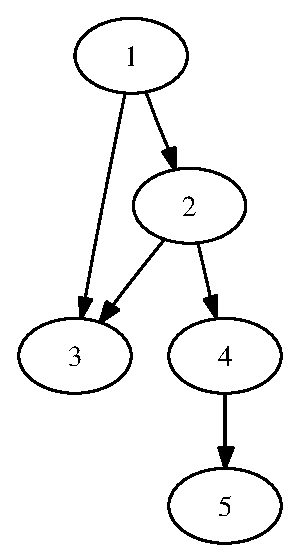
\epsfig{file=Figures/graph0,scale=0.6}
  \vspace*{-1cm}

  \caption{Ein einfacher Graph.}
  \label{fig:graph0}
\end{figure}



\noindent
In dem Graphen sind nur die unmittelbaren Verbindungen
zwischen zwei Punkten verzeichnet.  Es gibt aber unter Umst�nden auch noch
andere Verbindungen.  Beispielsweise gibt es eine unmittelbare Verbindung von
\texttt{1} nach \texttt{3}.  Es gibt dar�ber hinaus noch einen
Pfad von \texttt{1} nach \texttt{3}, der �ber den Punkt \texttt{2} geht.  
Unser Ziel in diesem Abschnitt ist es einen Algorithmus zu entwickeln, der �berpr�ft, ob
zwischen zwei Punkten eine Verbindung existiert und gegebenenfalls berechnet.
Dazu entwickeln wir zun�chst einen Algorithmus, der nur �berpr�ft, ob es eine
Verbindung zwischen zwei Punkten gibt und erweitern diesen Algorithmus dann sp�ter so, dass diese
Verbindung auch berechnet wird.

\subsection{Berechnung des transitiven Abschlusses einer Relation}
Als erstes bemerken wir, dass ein Graph $R$ nichts anderes ist als eine bin�re Relation.
Um feststellen zu k�nnen, ob es zwischen zwei Punkten eine Verbindung gibt,
m�ssen wir den transitiven Abschluss $R^+$ der Relation $R$ bilden.  Wir haben bereits
fr�her in dem Kapitel zur Mengenlehre gezeigt, dass $R^+$ wie folgt
berechnet werden kann: \\[0.2cm]
\hspace*{1.3cm} $R^+ = \bigcup\limits_{i=1}^{\infty} R^i = R \cup R^2 \cup R^3 \cup \cdots$  \\[0.2cm]
Auf den ersten Blick betrachtet sieht diese Formel so aus, als ob wir unendlich
lange rechnen m�ssten.  Aber versuchen wir einmal, diese Formel anschaulich zu
verstehen.  Zun�chst steht da $R$.  Das sind die Verbindungen, die unmittelbar  gegeben
sind.  Als n�chstes steht dort $R^2$ und das ist $R \circ R$.  Es gilt aber \\[0.2cm]
\hspace*{1.3cm} $R \circ R = \{ \pair(x,z) \mid \exists y \colon \pair(x,y) \in R \wedge \pair(y,z) \in R \}$
\\[0.2cm]
In $R^2$ sind also alle die Pfade enthalten, die aus zwei direkten Verbindungen
zusammengesetzt sind.  Allgemein l�sst sich durch Induktion sehen, dass $R^n$
alle die Pfade enth�lt, die aus $n$ direkten Verbindungen zusammengesetzt sind.  Nun
ist die Zahl der Punkte, die wir haben, endlich.  Sagen wir mal, dass es
$k$ Punkte sind.  Dann macht es  keinen Sinn solche Pfade zu betrachten, die
aus mehr als $k-1$ direkten Verbindungen zusammengesetzt sind, denn wir wollen ja
nicht im Kreis herum laufen.  Damit kann dann aber die Formel zur Berechnung des
transitiven Abschlusses vereinfacht werden:\\[0.2cm]
\hspace*{1.3cm} 
$R^+ = \bigcup\limits_{i=1}^{k-1} R^i$.
\\[0.2cm]
Diese Formel k�nnten wir tats�chlich so benutzen.  Es ist aber noch effizienter,
einen Fixpunkt-Algorithmus zu verwenden.  Dazu zeigen wir zun�chst, dass der transitive
Abschluss $R^+$ die folgende Fixpunkt-Gleichung erf�llt:
\begin{equation}
  \label{fixpunkt}
  R^+ = R \cup R \circ R^+. 
\end{equation}
Wir erinnern hier daran, dass wir vereinbart haben, dass der Operator $\circ$ st�rker
bindet als der Operator $\cup$, so dass der Ausdruck $R \cup R \circ R^+$ als
$R \cup (R \circ R^+)$ zu lesen ist.
Die Fixpunkt-Gleichung \ref{fixpunkt} l�sst sich algebraisch beweisen.  Es gilt
\[
\begin{array}{cll}
    & R \cup R \circ R^+ \\[0.2cm]
  = & R \cup R \circ \bigcup\limits_{i=1}^{\infty} R^i \\[0.4cm]
  = & R \cup R \circ \bigl(R^1 \cup R^2 \cup R^3 \cup \cdots \bigr) \\[0.2cm]
  = & R \cup \bigl(R \circ R^1 \cup R \circ R^2 \cup R \circ R^3 \cup \cdots \bigr) &
      \mbox{Distributiv-Gesetz} \\[0.2cm]
  = & R \cup \bigl(R^2 \cup R^3 \cup  R^4 \cup \cdots \bigr) & \mbox{Potenz-Gesetz} \\[0.2cm]
  = & R^1 \cup \bigl(R^2 \cup R^3 \cup  R^4 \cup \cdots \bigr) \\[0.2cm]
  = & \bigcup\limits_{i=1}^{\infty} R^i \\[0.4cm]
  = & R^+
\end{array}
\]
Die Gleichung \ref{fixpunkt} kann benutzt werden um den transitiven Abschluss iterativ zu
berechnen.  Wir definieren eine Folge $(T_n)_{n \in \mathbb{N}}$ durch Induktion folgt:
\begin{enumerate}
\item[I.A.] $n = 1$:         \hspace*{2.3cm} $T_1 := R$
\item[I.S.] $n \mapsto n+1$: \hspace*{1.6cm} $T_{n+1} := R \cup R \circ T_n$. 
\end{enumerate}
Die Relationen $T_n$ lassen sich auf die Relation $R$ zur�ckf�hren:
\begin{enumerate}
\item $T_1 = R$.
\item $T_2 = R \cup R \circ T_1 = R \cup R \circ R = R^1 \cup R^2$.
\item $\begin{array}[t]{lcl}
       T_3  & = & R \cup R \circ T_2 \\
            & = & R \cup R \circ (R^1 \cup R^2) \\
            & = & R^1 \cup R^2 \cup R^3. \\
       \end{array}
      $
\end{enumerate}
Allgemein k�nnen wir durch vollst�ndige Induktion �ber $n \in \mathbb{N}$ beweisen, dass
\[ T_n = \bigcup\limits_{i=1}^{n} R^i \]
gilt.  Der Induktions-Anfang folgt unmittelbar aus der Definition von $T_1$.  Um den 
Induktions-Schritt durchzuf�hren, betrachten wir
\[ \begin{array}{lcll}
   T_{n+1} & = & R \cup R \circ T_n & \mbox{gilt nach Definition} \\[0.2cm]
           & = & R \cup R \circ \left(\bigcup\limits_{i=1}^{n} R^i\right) &
                 \mbox{gilt nach Induktions-Voraussetzung} \\[0.4cm]
           & = & R \cup R^2 \cup \cdots \cup R^{n+1}  &
                 \mbox{Distributiv-Gesetz} \\[0.2cm]
           & = & R^1 \cup \cdots \cup R^{n+1} \\
           & = & \bigcup\limits_{i=1}^{n+1} R^i & \Box 
   \end{array}
\]
Die Folge $(T_n)_{n\in\mathbb{N}}$ hat eine weitere n�tzliche Eigenschaft: Sie ist 
\emph{monoton steigend}.  Allgemein nennen wir eine Folge von Mengen $(X_n)_{n\in\mathbb{N}}$
\emph{monoton steigend}, wenn 
\\[0.2cm]
\hspace*{1.3cm}
$\forall n \in \mathbb{N}: X_n \subseteq X_{n+1}$
\\[0.2cm]
gilt, wenn also die Mengen $X_n$ mit wachsendem Index $n$ immer gr��er werden.
Die Monotonie der Folge $(T_n)_{n \in \mathbb{N}}$ folgt aus der gerade bewiesenen Eigenschaft
$T_n = \bigcup_{i=1}^{n} R^i$, denn es gilt
\\[0.2cm]
\hspace*{1.3cm}
$
\begin{array}[t]{llcl}
                & T_n \subseteq T_{n+1} \\[0.2cm]
\Leftrightarrow & \bigcup\limits_{i=1}^{n} R^i \subseteq \bigcup\limits_{i=1}^{n+1} R^i \\[0.5cm]
\Leftrightarrow & \bigcup\limits_{i=1}^{n} R^i \subseteq \bigcup\limits_{i=1}^{n} R^i \cup R^{n+1} \\
\end{array}
$
\\[0.2cm]
und die letzte Formel ist offenbar wahr.  Ist nun die Relation $R$ endlich, so ist nat�rlich 
auch $R^+$ eine endliche Menge.  Da die 
Folge $T_n$ aber in dieser Menge liegt, denn es gilt ja 
\\[0.2cm]
\hspace*{1.3cm}
$T_n = \bigcup\limits_{i=1}^{n} R^i \subseteq \bigcup\limits_{i=1}^{\infty} R^i = R^+$ \quad f�r alle $n \in \mathbb{N}$,
\\[0.2cm]
k�nnen die Mengen $T_n$ nicht beliebig gro� werden.  Aufgrund der Monotonie der Folge
$(T_n)_{n\in\mathbb{N}}$ muss es daher einen Index $k$ geben, ab dem die Mengen $T_n$ alle gleich sind:
\\[0.2cm]
\hspace*{1.3cm}
$\forall n \in \mathbb{N}:( n \geq k \rightarrow T_n = T_k)$.
\\[0.2cm]
Ber�cksichtigen wir die Gleichung $T_n = \bigcup_{i=1}^{n} R^i$, so haben wir 
\\[0.2cm]
\hspace*{1.3cm}
$T_n = \bigcup\limits_{i=1}^{n} R^i = \bigcup\limits_{i=1}^{k} R^i = T_k$ \quad f�r alle $n \geq k$.
\\[0.2cm]
Daraus folgt dann aber, dass
\\[0.2cm]
\hspace*{1.3cm}
$T_n = \bigcup\limits_{i=1}^{n} R^i = \bigcup\limits_{i=1}^{\infty} R^i = R^+$ 
\quad f�r alle $n \geq k$  
\\[0.2cm]
gilt.  Der Algorithmus zur Berechnung von $R^+$ sieht nun so aus, dass wir die Iteration
\[ T_{n+1} := R \cup R \circ T_n \]
solange durchf�hren bis $T_{n+1} = T_n$ gilt, denn dann gilt auch $T_n = R^+$.


\begin{figure}[!ht]
  \centering
\begin{Verbatim}[ frame         = lines, 
                  framesep      = 0.3cm, 
                  labelposition = bottomline,
                  numbers       = left,
                  numbersep     = -0.2cm,
                  xleftmargin   = 0.8cm,
                  xrightmargin  = 0.8cm,
                ]
    closure := procedure(r) {
        t := r;
        while (true) {
            oldT := t;
            t    := r + product(r, t);
            if (t == oldT) {
                return t;
            }
        }
    };
    product := procedure(r1, r2) {
        return { [x,z] : [x,y] in r1, [y,z] in r2 };
    };
    r := { [1,2], [2,3], [1,3], [2,4], [4,5] };
    print( "r = ", r );
    print( "computing transitive closure of r" );
    t := closure(r);
    print( "r+ = ", t );
\end{Verbatim} 
\vspace*{-0.3cm}
\caption{Berechnung des transitiven Abschlusses.}  
\label{fig:transitive-closure.stlx}
\end{figure} %\$

\noindent
Das Programm 
\href{http://wwwlehre.dhbw-stuttgart.de/stroetmann/Logic/SetlX/transitive-closure.stlx}{\texttt{transitive-closure.stlx}}
in Abbildung
\ref{fig:transitive-closure.stlx} auf Seite \pageref{fig:transitive-closure.stlx}  zeigt
eine Implementierung dieses Gedankens.
Lassen wir dieses Programm laufen, so erhalten wir als Ausgabe:
\begin{verbatim}
    R = {[2, 3], [4, 5], [1, 3], [2, 4], [1, 2]}
    R+ = {[1, 5], [2, 3], [4, 5], [1, 4], [1, 3], [2, 4], [1, 2], [2, 5]}
\end{verbatim}
Der transitive Abschluss $R^+$ der Relation $R$ l�sst sich jetzt anschaulich
interpretieren:  Er enth�lt alle Paare $\pair(x,y)$, f�r die es einen \emph{Pfad} von
$x$ nach $y$ gibt.  Ein Pfad von $x$ nach $y$ ist dabei eine Liste der
Form \\[0.2cm]
\hspace*{1.3cm} $\bigl[ x_1, x_2, \cdots, x_n \bigr]$,
\\[0.2cm]
f�r die $x = x_1$ und $y = x_n$ gilt und f�r die au�erdem 
\\[0.2cm]
\hspace*{1.3cm}
$\pair(x_i, x_{i+1}) \in R$ \quad f�r alle $i = 1, \cdots, n-1$ gilt.
\\[0.2cm]
Die Funktion $\textsl{product}(r_1, r_2)$ berechnet das relationale Produkt $r_1 \circ
r_2$ nach der Formel
\\[0.2cm]
\hspace*{1.3cm}
$r_1 \circ r_2 = \{ \langle x, z \rangle \mid \exists y: \pair(x,y) \in r_1 \wedge \pair(y,z) \in r_2 \}$.
\\[0.2cm]
Die Implementierung dieser Prozedur  zeigt die allgemeine
Form der Mengen-Defi\-nition durch Iteratoren in \textsc{SetlX}.  Allgemein k�nnen wir eine Menge
durch den Ausdruck
\\[0.2cm]
\hspace*{1.3cm}
$\{\; \textsl{expr} \;\texttt{:}\; [x^{(1)}_1, \cdots, x^{(1)}_{n(1)}] \;\texttt{in}\; s_1,
     \cdots, [x^{(k)}_1, \cdots, x^{(k)}_{n(k)}] \;\texttt{in}\; s_k \;\texttt{|}\;
     \textsl{cond} \;\}
$
\\[0.2cm]
definieren.  Dabei muss $s_i$ f�r alle $i=1, \cdots, k$ eine Menge von Listen  der L�nge
$n(i)$ sein.  Bei der Auswertung dieses Ausdrucks werden f�r die Variablen 
$x^{(i)}_1, \cdots, x^{(i)}_{n(i)}$ die Werte eingesetzt, die die entsprechenden
Komponenten der Listen haben, die in der Menge $s_i$ auftreten.  Beispielsweise w�rde die
Auswertung von 
\begin{verbatim}
    s1 := { [ 1, 2, 3 ], [ 5, 6, 7 ] };
    s2 := { [ "a", "b" ], [ "c", "d" ] };
    m := { [ x1, x2, x3, y1, y2 ] : [ x1, x2, x3 ] in s1, [ y1, y2 ] in s2 };
\end{verbatim}
f�r \texttt{M} die Menge
\begin{verbatim}
    { [1, 2, 3, "a", "b"], [5, 6, 7, "c", "d"],  
      [1, 2, 3, "c", "d"], [5, 6, 7, "a", "b"] }
\end{verbatim}
berechnen. 


\subsection{Berechnung der Pfade}
Als n�chstes wollen wir das Programm zur Berechnung des transitiven Abschlusses so
erweitern, dass wir nicht nur feststellen k�nnen, dass es einen Pfad zwischen zwei Punkten
gibt, sondern dass wir diesen auch berechnen k�nnen.  Die Idee ist, dass wir statt des
relationalen Produkts, das f�r zwei Relationen definiert ist, ein sogenanntes
\emph{Pfad-Produkt}, das auf Mengen von Pfaden definiert ist, berechnen.  Vorab f�hren wir
f�r Pfade, die wir ja durch Listen repr�sentieren,
drei Begriffe ein.
\begin{enumerate}
\item Die Funktion $\textsl{first}(p)$ liefert den ersten Punkt der Liste $p$: \\[0.2cm]
      \hspace*{1.3cm} $\textsl{first}\bigl([x_1,\cdots,x_m]\bigr) = x_1$.
\item Die Funktion $\textsl{last}(p)$ liefert den letzten Punkt der Liste $p$: \\[0.2cm]
      \hspace*{1.3cm} $\textsl{last}\bigl([x_1,\cdots,x_m]\bigl) = x_m$.
\item Sind $p = [ x_1, \cdots, x_m ]$ und $q =[ y_1, \cdots, y_n ]$ 
      zwei Pfade mit $\textsl{first}(q) = \textsl{last}(p)$, dann definieren wir 
      die Summe von $p$ und $q$       als \\[0.2cm]
      \hspace*{1.3cm}
      $p \oplus q := [x_1, \cdots, x_m, y_2, \cdots, y_n ]$.
\end{enumerate}
Sind nun $P_1$ und $P_2$ Mengen von Pfaden, so definieren wir das  \emph{Pfad-Produkt} von
$P_1$ und $P_2$ als \\[0.2cm]
\hspace*{1.3cm} 
$P_1 \bullet P_2 := \bigl\{\; p_1 \oplus p_2 \mid p_1 \in P_1 \wedge p_2 \in P_2 \wedge \textsl{last}(p_1) = \textsl{first}(p_2) \;\bigr\}$.

\begin{figure}[!ht]
  \centering
\begin{Verbatim}[ frame         = lines, 
                  framesep      = 0.3cm, 
                  labelposition = bottomline,
                  numbers       = left,
                  numbersep     = -0.2cm,
                  xleftmargin   = 0.8cm,
                  xrightmargin  = 0.8cm,
                ]
    closure := procedure(r) {
        p := r;
        while (true) {
            oldP := p;
            p    := r + pathProduct(r, p);
            if (p == oldP) {
                return p;
            }
        }
    };
    pathProduct := procedure(p, q) {
        return { add(x, y) : x in p, y in q | x[#x] == y[1] };
    };    
    add := procedure(p, q) {
        return p + q[2..];
    };    
    r := { [1,2], [2,3], [1,3], [2,4], [4,5] };
    print( "r = ", r );
    print( "computing all paths" );
    p := closure(r);
    print( "p = ", p );
\end{Verbatim} 
\vspace*{-0.3cm}
\caption{Berechnung aller Verbindungen.}  \label{path.stlx}
\end{figure} %\$

\begin{figure}[!ht]
  \centering
  \vspace*{-9cm}

  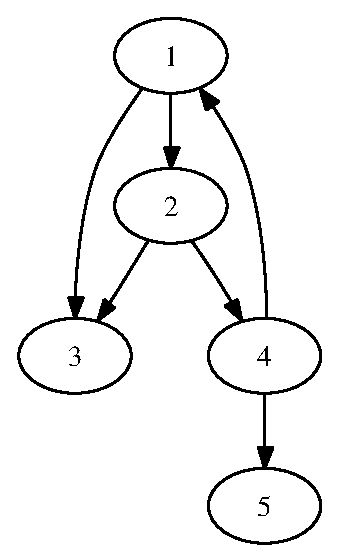
\epsfig{file=Figures/graph-zykl,scale=0.5}
  \vspace*{-1cm}

  \caption{Ein zyklischer Graph.}
  \label{fig:graph-zykl}
\end{figure}

Damit k�nnen wir das Programm in Abbildung
\ref{fig:transitive-closure.stlx} so ab�ndern, dass alle m�glichen Verbindungen zwischen zwei
Punkten berechnet werden.  Abbildung
\ref{path.stlx} zeigt das resultierende Programm
\href{http://wwwlehre.dhbw-stuttgart.de/stroetmann/Logic/SetlX/path.stlx}{\texttt{path.stlx}}. 
Leider funktioniert das Programm dann nicht mehr, wenn der Graph Zyklen enth�lt.
Abbildung
\ref{fig:graph-zykl} zeigt einen Graphen, der einen Zyklus enth�lt.  In diesem Graphen
gibt es unendlich viele Pfade, die von dem Punkt 1 zu dem Punkt 2 f�hren: \\[0.2cm]
\hspace*{1.3cm} $[ 1, 2 ]$, $[ 1, 2, 4, 1, 2 ]$, 
$[ 1, 2, 4, 1, 2, 4, 1, 2 ]$, 
$[ 1, 2, 4, 1, 2, 4, 1, 2, 4, 1, 4 ]$, $\cdots$
\\[0.2cm]
Offenbar  sind die Pfade unwichtig, die einen Punkt mehrfach enthalten und die daher
zyklisch sind.  Solche Pfade sollten wir bei der Berechnung des Pfad-Produktes
eliminieren.

\begin{figure}[!ht]
  \centering
\begin{Verbatim}[ numbers       = left,
                  numbersep     = -0.2cm,
                  frame         = lines, 
                  framesep      = 0.3cm, 
                  labelposition = bottomline,
                  xleftmargin   = 0.0cm,
                  xrightmargin  = 0.0cm,
                ]
    pathProduct := procedure(p, q) {
        return { add(x,y) : x in p, y in q | x[#x] == y[1] && noCycle(x,y) };
    };
    noCycle := procedure(l1, l2) {
        return #({ x : x in l1 } * { x : x in l2 }) == 1;
    };
\end{Verbatim} 
\vspace*{-0.3cm}
\caption{Berechnung aller Verbindungen in zyklischen Graphen}  
\label{fig:path-cyclic.stlx}
\end{figure} %\$

Abbildung \ref{fig:path-cyclic.stlx} zeigt einen Ausschnitt des ge�nderten Programms
\href{http://wwwlehre.dhbw-stuttgart.de/stroetmann/Logic/SetlX/path-cyclic.stlx}{\texttt{path-cyclic.stlx}},
das auch f�r zyklische Graphen funktioniert. 
\begin{enumerate}
\item In Zeile 2 ber�cksichtigen wir nur die Pfade $x \oplus y$, die nicht zyklisch sind.
\item In Zeile 5 �berpr�fen wir, ob die Konkatenation  $l_1 \oplus l_2$ zyklisch ist.  Die
      Kombination von $l_1$ und $l_2$  ist genau dann 
      zyklisch, wenn die Listen $l_1$ und $l_2$ mehr als ein gemeinsames Element
      enthalten.  Die Listen $l_1$ und $l_2$ enthalten mindestens ein gemeinsames Element,
      denn wir verkn�pfen diese beiden Listen ja nur dann, wenn das letzte Element
      der Liste $l_1$ mit dem ersten Element der Liste $l_2$ �bereinstimmt.
      Wenn es nun noch einen weiteren Punkt geben w�rde, der sowohl in $l_1$ als auch in
      $l_2$ auftreten w�rde, dann w�re der Pfad $l_1 \oplus l_2$ zyklisch.
\end{enumerate}

In den meisten F�llen sind wird gar nicht daran interessiert, alle m�glichen Verbindungen
zwischen allen Punkten zu berechnen, das w�re n�mlich viel zu aufwendig, sondern wir
wollen nur zwischen zwei gegebenen Punkten 
eine Verbindung finden.  Abbildung \ref{fig:find-path} zeigt die Implementierung einer
Prozedur $\texttt{reachable}(x, y, r)$, die �berpr�ft, ob es in dem Graphen $r$ eine
Verbindung von $x$ nach $y$ gibt und die diese Verbindung berechnet.  Das vollst�ndige
Programm finden Sie in der Datei
\href{http://wwwlehre.dhbw-stuttgart.de/stroetmann/Logic/SetlX/find-path.stlx}{\texttt{find-path.stlx}}.
Wir diskutieren nun die Implementierung der Prozedur \texttt{reachable}.
\begin{enumerate}
\item In Zeile 2 initialisieren wir $p$ so, dass zun�chst nur der Pfad der L�nge 0,
      der mit dem Punkt $x$  startet, in $p$ liegt.
\item In Zeile 6 selektieren wir die Pfade aus $p$, die zum Ziel $y$ f�hren.
\item Wenn wir dann in Zeile 7 feststellen, dass wir einen solchen Pfad berechnet haben,
      geben wir einen dieser Pfade in Zeile 8 zur�ck.
\item Falls es nicht gelingt einen solchen Pfad zu berechnen und wir keine neuen
      Pfade mehr finden k�nnen, verlassen wir die Prozedur in Zeile 11
      mit dem Befehl \texttt{return}.  Da wir bei diesem \texttt{return}-Befehl
      keinen Wert zur�ckgeben, ist der R�ckgabewert der Prozedur in diesem Fall
      automatisch $\Omega$.
\end{enumerate}

\begin{figure}[!ht]
  \centering
\begin{Verbatim}[ frame         = lines, 
                  framesep      = 0.3cm, 
                  labelposition = bottomline,
                  numbers       = left,
                  numbersep     = -0.2cm,
                  xleftmargin   = 0.8cm,
                  xrightmargin  = 0.8cm,
                ]
    reachable := procedure(x, y, r) {
        p := { [x] };
        while (true) {
            oldP  := p;
            p     := p + pathProduct(p, r);
            found := { l in p | l[#l] == y };
            if (found != {}) {
                return arb(found);
            }
            if (p == oldP) {
                return;
            }
        }
    };
\end{Verbatim} 
\vspace*{-0.3cm}
\caption{Berechnung aller Verbindungen zwischen zwei Punkten}  
\label{fig:find-path}
\end{figure} %\$

\subsection{Der Bauer mit dem Wolf, der Ziege und dem Kohl}
Wir pr�sentieren nun eine betriebswissenschaftliche Anwendung des oben entwickelten Algorithmus und
betrachten folgendes Problem.
\vspace*{0.3cm}

\begin{minipage}[c]{14cm}
{\sl
Ein Agrar�konom will mit einem Wolf, einer Ziege und einem Kohl �ber einen Fluss �bersetzen, um
diese als Waren auf dem Markt zu verkaufen.
Das Boot ist aber so klein, dass er nicht mehr als zwei Waren gleichzeitig mitnehmen kann.
Wenn der Bauer den Wolf mit der Ziege allein l�sst, dann frisst der Wolf die Ziege und wenn er die
Ziege mit dem Kohl allein l�sst, dann frisst die Ziege den Kohl. }
\end{minipage}
\vspace*{0.3cm}

\noindent
Wir wollen einen Fahrplan entwickeln, mit dem der Agrar�konom alle seine Waren unbeschadet zum
Markt bringen kann.  Dazu modellieren wir das R�tsel als Erreichbarkeits-Problem in einem
Graphen.  
Die Punkte des Graphen beschreiben dabei die einzelnen Situationen, die auftreten
k�nnen.  Wir definieren eine Menge\\[0.2cm]
\hspace*{1.3cm} 
$\texttt{all} := \{ \squote{Bauer}, \squote{Wolf}, \squote{Ziege},\squote{Kohl} \}$.
\\[0.2cm]
Die einzelnen Punkte sind dann Paare von Mengen, haben also die Form \\[0.2cm]
\hspace*{1.3cm} 
$\langle s_1, s_2 \rangle$ \quad mit $s_1,s_2 \subseteq \texttt{all}$.
\\[0.2cm]
Dabei gibt die Menge $s_1$ an, was am linken Ufer ist und $s_2$ gibt an, was am rechten
Ufer ist.  Die Menge aller Punkte k�nnen wir dann definieren als \\[0.2cm]
\hspace*{1.3cm} 
$p := \bigl\{ \langle s_1, s_2 \rangle \in 2^\texttt{all} \times 2^\texttt{all} \;|\;
              s_1 \cup s_2 = \texttt{all} \;\wedge\; s_1 \cap s_2 = \{\} 
      \bigr\}
$.
\\[0.2cm]
Die Bedingung $s_1 \cup s_2 = \texttt{all}$ stellt dabei sicher, dass nichts verloren
geht:  Jedes der Elemente aus \texttt{all} ist entweder am linken oder am rechten Ufer.
Die Bedingung $s_1 \cap s_2 = \{\}$ verbietet die Bilokalisation von Objekten, sie stellt also sicher,
dass kein Element aus der Menge \texttt{all}  gleichzeitig am  linken und am rechten Ufer ist.

Als n�chstes definieren wir den Graphen $r$, also die m�glichen Verbindungen zwischen
Punkten.  Dazu definieren wir eine Prozedur $\textsl{problem}(s)$. Hierbei ist $s$ eine
Menge von Objekten, die an einem Ufer sind.  Die Prozedur $\textsl{problem}(s)$
liefert genau dann \texttt{true}, wenn es bei der  Menge $s$ ein Problem gibt, weil entweder die Ziege
mit dem Kohl allein ist, oder aber der Wolf die Ziege frisst.
\begin{verbatim}
    problem := procedure(s) {
        return "goat" in s && "cabbage" in s || "wolf" in s && "goat" in s;
    };
\end{verbatim}
Damit k�nnen wir eine Relation $r_1$ wie folgt definieren:
\\[0.2cm]
\hspace*{1.3cm} 
$r_1 := \Bigl\{ \bigl\langle \pair(s_1, s_2), \pair(s_1 \backslash b, s_2 \cup b)
  \bigr\rangle \;|\; $ \\
\hspace*{2.3cm} 
$\pair(s_1, s_2) \in P \;\wedge\; b \subseteq s_1 \;\wedge\;
 \squote{Bauer} \in b \;\wedge\; \textsl{card}(b) \leq 2 \;\wedge\; \neg\textsl{problem}(s_1 \backslash b) \Bigr\}$.
\\[0.2cm]
Diese Menge beschreibt alle die Fahrten, bei denen der Bauer vom linken Ufer zum rechten Ufer
f�hrt und bei denen zus�tzlich sichergestellt ist, dass am linken Ufer
nach der �berfahrt kein Problem auftritt.  Die einzelnen Terme werden wie folgt
interpretiert:
\begin{enumerate}
\item $\pair(s_1,s_2)$ ist der Zustand vor der �berfahrt des Bootes,
      $s_1$ gibt also die Objekte am linken Ufer an, $s_2$ sind die Objekte am rechten Ufer.
\item $b$ ist der Inhalt des Bootes, daher beschreibt 
       $\pair(s_1 \backslash b, s_2 \cup b)$ den Zustand nach der �berfahrt des Bootes:
       Links sind nun nur noch die Objekte aus $s_1 \backslash b$, daf�r sind rechts dann 
       die Objekte $s_2 \cup b$.

       Die Bedingungen lassen sich wie folgt interpretieren.
\item $b \subseteq s_1$: Es k�nnen nat�rlich nur solche Objekte ins Boot genommen werden,
       die vorher am linken Ufer waren.
\item $\squote{Bauer} \in b$: Der Bauer muss auf jeden Fall ins Boot, denn weder der Wolf
       noch die Ziege k�nnen rudern.
\item $\textsl{card}(b) \leq 2$: Die Menge der Objekte im Boot darf nicht mehr als zwei
       Elemente haben, denn im Boot ist nur f�r zwei Platz.
\item $\neg\textsl{problem}(s_1 \backslash b)$:  Am linken Ufer soll es nach der �berfahrt
       kein Problem geben, denn der Bauer ist ja hinterher am rechten Ufer.
\end{enumerate}
In analoger Weise definieren wir nun eine Relation $r_2$ die die �berfahrten vom rechten
Ufer zum linken Ufer beschreibt:\\[0.2cm]
\hspace*{1.3cm} 
$r_2 := \Bigl\{ \bigl\langle \pair(s_1, s_2), \pair(s_1 \cup b, s_2 \backslash b)
  \bigr\rangle \;|\; $ \\
\hspace*{2.3cm} 
$\pair(s_1, s_2) \in P \;\wedge\; b \subseteq s_2 \;\wedge\;
 \squote{Bauer} \in b \;\wedge\; \textsl{card}(b) \leq 2 \;\wedge\; \neg\textsl{problem}(s_2 \backslash b) \Bigr\}$.
\\[0.2cm]
Die gesamte Relation $r$ definieren wir nun als
\\[0.2cm]
\hspace*{1.3cm} $r := r_1 \cup r_2$.\\[0.2cm]
Als n�chstes m�ssen wir den Start-Zustand modellieren.
Am Anfang sind alle am linken Ufer, also wird der Start-Zustand durch das Paar 
\\[0.3cm]
\hspace*{1.3cm}
$\bigl\langle \{ \squote{Bauer}, \squote{Wolf}, \squote{Ziege},\squote{Kohl} \}, \{\} \bigr\rangle$.
\\[0.3cm]
Beim Ziel ist es genau umgekehrt, dann sollen alle auf der rechten Seite des Ufers sein:
\\[0.3cm]
\hspace*{1.3cm}
$\bigl\langle \{\}, \{ \squote{Bauer}, \squote{Wolf}, \squote{Ziege},\squote{Kohl} \} \bigr\rangle$.
\\[0.3cm]
Damit haben wir das Problem in der Mengenlehre modelliert und k�nnen die im letzten
Abschnitt entwickelte Prozedur \texttt{reachable} benutzen, um das Problem zu l�sen.
In der Abbildung \ref{fig:wolf-ziege} finden Sie das Programm 
\href{http://wwwlehre.dhbw-stuttgart.de/stroetmann/Logic/SetlX/wolf-goat-cabbage.stlx}{\texttt{wolf-goat-cabbage.stlx}},
in dem die oben ausgef�hrten �berlegungen in \textsc{SetlX} umgesetzt wurden.
Die von diesem Programm berechnete L�sung finden Sie in Abbildung \ref{fig:wolf-ziege-solution}.

\begin{figure}[!ht]
  \centering
\begin{Verbatim}[ codes         = {\catcode`$=3\catcode`_=8\catcode`^=7},
                  frame         = lines, 
                  framesep      = 0.3cm, 
                  labelposition = bottomline,
                  numbers       = left,
                  numbersep     = -0.2cm,
                  xleftmargin   = 0.0cm,
                  xrightmargin  = 0.0cm,
                ]
    all := { "farmer", "wolf", "goat", "cabbage" };
    p   := pow(all);
    r1  := { [ s, s - b ] : s in p, b in pow(s) 
                          | "farmer" in b && #b <= 2 && !problem(s - b) 
           };
    r2  := { [ s, s + b ] : s in p, b in pow(all - s) 
                          | "farmer" in b && #b <= 2 && !problem(all - (s + b))
           };
    r   := r1 + r2;
    start := [ all, {} ];
    goal  := [ {}, all ];
    path := findPath(start, goal, r);
\end{Verbatim} 
\vspace*{-0.3cm}
\caption{Wie kommt der Bauer ans andere Ufer?}  
\label{fig:wolf-ziege}
\end{figure} %\$
\noindent

\begin{figure}[!ht]
  \centering
\begin{Verbatim}[ codes         = {\catcode`$=3\catcode`_=8\catcode`^=7},
                  frame         = lines, 
                  framesep      = 0.3cm, 
                  labelposition = bottomline,
                  numbers       = left,
                  numbersep     = -0.2cm,
                  commandchars  = \\\{\},
                  xleftmargin   = 0.0cm,
                  xrightmargin  = 0.0cm,
                ]
    \{"Kohl", "Ziege", "Wolf", "Bauer"\}                                        \{\}
                              >> \{"Ziege", "Bauer"\} >>
    \{"Kohl", "Wolf"\}                                          \{"Ziege", "Bauer"\}
                              << \{"Bauer"\} <<<< 
    \{"Kohl", "Wolf", "Bauer"\}                                          \{"Ziege"\}
                              >> \{"Wolf", "Bauer"\} >>>
    \{"Kohl"\}                                          \{"Ziege", "Wolf", "Bauer"\}
                              << \{"Ziege", "Bauer"\} <<
    \{"Kohl", "Ziege", "Bauer"\}                                          \{"Wolf"\}
                              >> \{"Kohl", "Bauer"\} >>>
    \{"Ziege"\}                                          \{"Kohl", "Wolf", "Bauer"\}
                              << \{"Bauer"\} <<<< 
    \{"Ziege", "Bauer"\}                                          \{"Kohl", "Wolf"\}
                              >> \{"Ziege", "Bauer"\} >>    
    \{\}                                        \{"Kohl", "Ziege", "Wolf", "Bauer"\}
\end{Verbatim} 
\vspace*{-0.3cm}
\caption{Ein Fahrplan f�r den Bauern}  
\label{fig:wolf-ziege-solution}
\end{figure} %$
\pagebreak

\vspace*{\fill}
\pagebreak

\section{Terme und Matching}
Neben den bisher vorgestellten Datenstrukturen gibt es noch eine weitere wichtige
Datenstruktur, die sogenannten \emph{Terme}, die insbesondere n�tzlich ist, wenn wir
\emph{symbolische Programme} 
schreiben wollen.  Darunter verstehen wir solche Programme, die Formeln manipulieren.
Wollen wir beispielsweise ein Programm schreiben, dass als Eingabe einen String wie
\\[0.2cm]
\hspace*{1.3cm}
``\texttt{x * sin(x)}''
\\[0.2cm]
einliest, diesen String als eine Funktion in der Variablen ``\texttt{x}'' interpretiert
und dann die Ableitung dieser Funktion nach der Variablen ``\texttt{x}'' berechnet, so
sprechen wir von einem \emph{symbolischen Programm}.   Wollen wir einen Ausdruck wie 
``\texttt{x * sin(x)}'' darstellen, so eignen sich \emph{Terme} am besten dazu.
Im n�chsten Unter-Abschnitt werden wir zun�chst \emph{Terme} zusammen mit den in \setl\
vordefinierten Funktionen vorstellen, die zur Verarbeitung von Termen benutzt werden k�nnen.
Anschlie�end stellen wir das sogenannte \emph{Matching} vor, mit dessen Hilfe sich Terme
besonders leicht manipulieren lassen.


\subsection{Konstruktion und Manipulation von Termen}
Terme werden mit Hilfe sogenannter \emph{Funktions-Zeichen} gebildet.  Es ist wichtig,
dass Sie Funktions-Zeichen nicht mit Funktionen oder Variablen verwechseln.  In \setl\
beginnen Funktionen-Zeichen im Gegensatz zu einem Variablen-Namen daher mit einem gro�en
Buchstaben.  Auf den Gro�buchstaben k�nnen  dann beliebig viele Buchstaben, Ziffern und
der Unterstrich ``\texttt{\_}'' folgen.
Zus�tzlich gibt es noch Funktionszeichen, die mit dem Zeichen
``\texttt{\symbol{94}}''
beginnen.  Solche Funktions-Zeichen werden intern von \setl\ verwendet um Operator-Symbole
wie ``\texttt{+}'' oder ``\texttt{*}'' darzustellen.
Die folgenden Strings k�nnen beispielsweise  als Funktions-Zeichen vewendet werden:
\\[0.2cm]
\hspace*{1.3cm}
\texttt{F}, \quad \texttt{FabcXYZ}, \quad \texttt{\symbol{94}sum}, \quad \texttt{Hugo\_}.
\\[0.2cm]
Damit sind wir nun in der Lage, Term zu definieren.  Ist $F$ ein Funktions-Zeichen und sind
$t_1$, $t_2$, $\cdots$, beliebige \setl-Werte, so ist der Ausdruck
\\[0.2cm]
\hspace*{1.3cm}
$F(t_1, t_2, \cdots, t_n)$
\\[0.2cm]
ein Term.  Beachten Sie, dass Terme ganz �hnlich aussehen wie die Aufrufe von Funktionen.
Terme und Aufrufe von Funktionen unterscheiden sich nur dadurch, dass bei einem Term links
vor der ersten �ffnenden Klammer ein Funktions-Zeichen steht, w�hrend bei einem
Funktions-Aufruf dort statt dessen eine Variable steht, der eine Funktions-Definition zugewiesen
worden ist.

\examples
\begin{enumerate}
\item \texttt{Adresse(\symbol{34}Roteb�hlplatz 41\symbol{34}, 70178, \symbol{34}Stuttgart\symbol{34})}

      ist ein Term, der eine Adresse repr�sentiert.
\item \texttt{Product(Variable(\symbol{34}x\symbol{34}), Sin(Variable(\symbol{34}x\symbol{34})))}

      ist ein Term, der einen arithmetischen Ausdruck repr�sentiert, den Sie mathematisch
      als $x * \sin(x)$ schreiben w�rden.  \eox
\end{enumerate}

An dieser Stelle fragen Sie sich vielleicht, wie Terme ausgewertet werden.  Die Antwort ist:
\textbf{Gar nicht!}  Terme werden nur dazu benutzt, Daten darzustellen.  Terme sind also bereits 
Werte  genauso wie auch Zahlen, Strings, Mengen oder Listen als Werte aufgefasst werden.
Genausowenig wie Sie die Zahl \texttt{42} auswerten m�ssen, m�ssen Sie einen Term auswerten.

Nehmen wir einmal an,
dass es in \setl\ keine Listen geben w�rde.  Dann k�nnten wir Listen als Terme darstellen.  Zun�chst
w�rden wir ein Funktions-Zeichen ben�tigen, mit dem wir die leere Liste darstellen k�nnten.  Wir
w�hlen dazu das Funktions-Zeichen \texttt{Nil}.  Damit haben wir dann also die Entsprechung
\\[0.2cm]
\hspace*{1.3cm}
$\texttt{Nil}() \;\widehat{=}\; \texttt{[]}$.
\\[0.2cm]
\textbf{Beachten} Sie hier, dass die Klammern hinter dem Funktions-Zeichen \texttt{Nil} nicht
weggelassen werden d�rfen!  Um nun eine Liste darzustellen, deren erstes Element $x$ ist und deren
restliche Elemente durch die Restliste $r$ gegeben sind, verwenden wir das Funktions-Zeichen
\texttt{Cons}.  Dann haben wir die Entsprechung
\\[0.2cm]
\hspace*{1.3cm}
$\texttt{Cons(x, r)} \;\widehat{=}\; \texttt{[}x\texttt{]}+r$. 
\\[0.2cm]
Konkret k�nnen wir nun die Liste \texttt{[1,2,3]} durch den Term
\\[0.2cm]
\hspace*{1.3cm}
\texttt{Cons(1, Cons(2, Cons(3, Nil())))}
\\[0.2cm]
darstellen.  In der Sprache \textsl{Prolog}, die wir sp�ter noch besprechen werden, werden Listen
intern �brigens in �hnlicher Form als Terme dargestellt.

Es gibt zwei vordefinierte Funktionen in \setl, mit denen wir auf die Komponenten eines Terms
zugreifen k�nnen und es gibt eine Funktion, mit deren Hilfe wir Terme konstruieren k�nnen.
\begin{enumerate}
\item Die Funktion \texttt{fct} berechnet das Funktions-Zeichen eines Terms.
      Falls $t$ ein Term der Form $F(s_1,\cdots,s_n)$ ist, so ist das Ergebnis des Funktions-Aufrufs
      \\[0.2cm]
      \hspace*{1.3cm}
      $\texttt{fct}(F(s_1,\cdots,s_n))$
      \\[0.2cm]
      das Funktions-Zeichen $F$ dieses Terms.  Beispielsweise liefert der Ausdruck
      \\[0.2cm]
      \hspace*{1.3cm}
      \texttt{fct(Cons(1, Cons(2, Cons(3, Nil()))))}
      \\[0.2cm]
      als Ergebnis das Funktions-Zeichen \texttt{\symbol{34}Cons\symbol{34}}.
\item Die Funktion \texttt{args} berechnet die Argumente eines Terms.
      Falls $t$ ein Term der Form $F(s_1,\cdots,s_n)$ ist, dann liefert der Ausdruck
      \\[0.2cm]
      \hspace*{1.3cm}
      $\mathtt{args}(F(s_1,\cdots,s_n))$
      \\[0.2cm]
      als Ergebnis die Liste $[s_1, \cdots, s_n]$ der Argumente des Terms $t$  .  Beispielsweise
      liefert der Ausdruck
      \\[0.2cm]
      \hspace*{1.3cm}
      \texttt{args(Cons(1, Cons(2, Cons(3, Nil()))))}
      \\[0.2cm]
      das Ergebnis
      \\[0.2cm]
      \hspace*{1.3cm}
      \texttt{[1, Cons(2, Cons(3, Nil()))]}.
\item Ist ein Funktions-Zeichen $f$ und eine Liste $l$ von Argumenten gegeben, so erzeugt die
      Funktion \texttt{makeTerm} durch den Aufruf
      \\[0.2cm]
      \hspace*{1.3cm}
      $\texttt{makeTerm}(f,l)$
      \\[0.2cm]
      einen Term $t$ mit dem Funktions-Zeichen $f$ und der Argument-Liste $l$, f�r $t$ gilt also
      \\[0.2cm]
      \hspace*{1.3cm}
      $\mathtt{fct}(t) = f$  \quad und \quad $\mathtt{args}(t) = l$.
      \\[0.2cm]
      Beispielsweise liefert der Aufruf
      \\[0.2cm]
      \hspace*{1.3cm}
      \texttt{makeTerm(\symbol{34}Cons\symbol{34}, [ 1, Nil() ])}
      \\[0.2cm]
      als Ergebnis den Term
      \\[0.2cm]
      \hspace*{1.3cm}
      \texttt{Cons(1,Nil())}.
      \\[0.2cm]
      Diesen Term h�tten wir nat�rlich auch unmittelbar hinschreiben k�nnen.
\end{enumerate}

\begin{figure}[!ht]
\centering
\begin{Verbatim}[ frame         = lines, 
                  framesep      = 0.3cm, 
                  firstnumber   = 1,
                  labelposition = bottomline,
                  numbers       = left,
                  numbersep     = -0.2cm,
                  xleftmargin   = 0.8cm,
                  xrightmargin  = 0.8cm,
                ]
    append := procedure(l, x) {
        if (fct(l) == "Nil") {
            return Cons(x, Nil());
        }
        [head, tail] := args(l);
        return Cons(head, append(tail, x));
    };
\end{Verbatim}
\vspace*{-0.3cm}
\caption{Einf�gen eines Elements am Ende einer Liste.}
\label{fig:append.stlx}
\end{figure}

In Abbildung  \ref{fig:append.stlx} auf Seite \pageref{fig:append.stlx} sehen Sie die
Implementierung  einer Funktion
\href{http://wwwlehre.dhbw-stuttgart.de/stroetmann/Logic/SetlX/append.stlx}{\texttt{append}},
deren Aufgabe es ist, ein Element $x$ am Ende einer Liste $l$ einzuf�gen, wobei vorausgesetzt ist,
dass die Liste $l$ als Term mit Hilfe der Funktions-Zeichen ``\texttt{Cons}'' und ``\texttt{Nil}''
dargestellt wird.
\begin{enumerate}
\item Zun�chst wird in Zeile 2 �berpr�ft, ob die Liste $l$ leer ist.  Die Liste $l$ ist genau dann
      leer, wenn $l = \texttt{Nil()}$ gilt.  Daher k�nnen wir einfach das Funktions-Zeichen von dem
      Term $l$ testen um herauszufinden, ob $l$ die leere Liste repr�sentiert.
\item Falls $l$ nicht leer ist, muss $l$ die Form
      \\[0.2cm]
      \hspace*{1.3cm}
      $l = \texttt{Cons(\textsl{head}, \textsl{tail})}$
      \\[0.2cm]     
      haben.  Dann ist \textsl{head} das erste Element der Liste $l$ und \textsl{tail} bezeichnet
      die Liste der restlichen Elemente.  In diesem Fall m�ssen wir $x$ rekursiv in die Liste
      \textsl{tail} einf�gen.  Als Ergebnis wird in Zeile 6 dann eine neue Liste erzeugt, deren
      erstes Element \textsl{head} ist, w�hrend die Liste der restlichen Elemente durch den
      rekursiven Aufruf von \textsl{append} berechnet wird.
\end{enumerate}
In manchen F�llen ist es sehr unbequem, dass Funktions-Zeichen immer mit einem gro�en Buchstaben
beginnen m�ssen.  Deswegen gibt es in \setl\ einen Escape-Mechanismus, der es erlaubt, auch
Funktionszeichen zu verwenden, die mit einem kleinen Buchstaben beginnen:  Falls wir einem
Funktionszeichen den Operator ``\texttt{\symbol{64}}'' voranstellen, dann darf das Funktionszeichen
auch mit einem kleinen Buchstaben beginnen.  Wollen wir beispielsweise Terme benutzen um
algebraische Ausdr�cke darzustellen, die trigonometrische Funktionen enthalten, 
so k�nnen wir einen Ausdruck der Form $\sin(x)$ durch den Term
\\[0.2cm]
\hspace*{1.3cm}
\texttt{\symbol{64}sin(\symbol{34}x\symbol{34})}  
\\[0.2cm]
darstellen.

\subsection{Matching}
Der Umgang mit Termen w�re sehr m�hsam, wenn wir die Terme jedesmal mit Hilfe der Funktionen
\texttt{fct} und \texttt{args} auseinander nehmen m�ssten.  Abbildung \ref{fig:append-match.stlx} 
zeigt eine weitere Implementierung der Funktion
\href{http://wwwlehre.dhbw-stuttgart.de/stroetmann/Logic/SetlX/append-match.stlx}{\texttt{append}}, 
bei der wir die Kontroll-Struktur \texttt{match} an Stelle der Funktionen ``\texttt{fct}''
and ``\texttt{args}'' verwendet haben.  In Zeile 3 wird  �berpr�ft, ob die Liste $l$ leer ist.
Die wahre St�rke des Matchings sehen wir allerdings ist in Zeile 4, denn dort wird nicht nur
�berpr�ft, ob die Liste $l$ die Form
\\[0.2cm]
\hspace*{1.3cm}
\texttt{Cons(\textsl{head},\textsl{tail})}
\\[0.2cm]
hat, sondern gleichzeitig werden die Variablen \textsl{head} and \textsl{tail} so gesetzt, dass
anschlie�end die Gleichung
\\[0.2cm]
\hspace*{1.3cm}
$l = \texttt{Cons(\textsl{head},\textsl{tail})}$
\\[0.2cm]
erf�llt ist.


\begin{figure}[!ht]
\centering
\begin{Verbatim}[ frame         = lines, 
                  framesep      = 0.3cm, 
                  firstnumber   = 1,
                  labelposition = bottomline,
                  numbers       = left,
                  numbersep     = -0.2cm,
                  xleftmargin   = 0.8cm,
                  xrightmargin  = 0.8cm,
                ]
    append := procedure(l, x) {
        match (l) {
            case Nil():            return Cons(x, Nil());
            case Cons(head, tail): return Cons(head, append(tail, x));
        }
    };
\end{Verbatim}
\vspace*{-0.3cm}
\caption{Implementierung von \texttt{append} mit Hilfe von \emph{Matching}.}
\label{fig:append-match.stlx}
\end{figure}

Im Allgemeinen ist  ein \texttt{match}-Block so �hnlich aufgebaut wie ein
\texttt{switch}-Block und hat die in Abbildung \ref{fig:match} gezeigte Struktur.
Hier bezeichnet $e$ einen Ausdruck, dessen Auswertung einen Term ergibt.  
Die Ausdr�cke $t_1$, $\cdots$, $t_n$ sind sogenannte \emph{Muster}, die freie
Variablen enthalten.  Bei der Auswertung eines \texttt{Match}-Blocks versucht
\textsc{SetlX} die in dem Muster $t_i$ auftretenden Variablen so zu setzen, dass das Muster
zu dem Ergebnis der Auswertung von $e$ gleich ist.  Gelingt dies, so wird die
mit $\textsl{body}_i$ bezeichnete Gruppe von Befehlen ausgef�hrt.  Andernfalls
versucht \textsc{SetlX} das n�chste Muster $t_{i+1}$ mit $e$ zur Deckung zu bringen.
Falls keines der Muster $t_1$, $\cdots$, $t_n$ mit $e$ zur Deckung zu bringen ist, wird
ersatzweise $\textsl{body}_{n+1}$ ausgef�hrt.  

\begin{figure}[!ht]
  \centering
\begin{Verbatim}[ codes         = {\catcode`_=8\catcode`^=7},
                  frame         = lines, 
                  framesep      = 0.3cm, 
                  labelposition = bottomline,
                  numbers       = left,
                  numbersep     = -0.2cm,
                  commandchars  = \\\{\},
                  xleftmargin   = 0.8cm,
                  xrightmargin  = 0.8cm
                ]
      \texttt{\underline{match} (\(e\)) \{}
          \texttt{\underline{case}} \(t_1\) : \textsl{body}\(_1\) 
          \vdots
          \texttt{\underline{case}} \(t_n\) : \textsl{body}\(_n\)
          \texttt{\underline{default}:} \textsl{body}\(_{n+1}\)
      \texttt{\}}
\end{Verbatim}
\vspace*{-0.3cm}
\caption{Struktur eines \texttt{Match}-Blocks}  \label{fig:match}
\end{figure} 


\begin{figure}[!ht]
\centering
\begin{Verbatim}[ frame         = lines, 
                  framesep      = 0.3cm, 
                  firstnumber   = 1,
                  labelposition = bottomline,
                  numbers       = left,
                  numbersep     = -0.2cm,
                  xleftmargin   = 0.8cm,
                  xrightmargin  = 0.8cm,
                ]
    diff := procedure(t, x) {
        match (t) {
            case t1 + t2 :
                return diff(t1, x) + diff(t2, x);
            case t1 - t2 :
                return diff(t1, x) - diff(t2, x);
            case t1 * t2 :
                return diff(t1, x) * t2 + t1 * diff(t2, x);
            case t1 / t2 :
                return ( diff(t1, x) * t2 - t1 * diff(t2, x) ) / t2 * t2;
            case f ** g :
                return diff( @exp(g * @ln(f)), x);
            case ln(a) :
                return diff(a, x) / a;
            case exp(a) :
                return diff(a, x) * @exp(a);
            case ^variable(x) : // x is defined above as second argument
                return 1;
            case ^variable(y) : // y not yet defined, matches any other variable
                return 0;
            case n | isNumber(n):   
                return 0;  
        }
    };
\end{Verbatim}
\vspace*{-0.3cm}
\caption{A function to perform symbolic differentiation.}
\label{fig:diff.stlx}
\end{figure}

\noindent
Wir zeigen zum Abschluss dieses Abschnitts ein komplexeres Beispiel.  Die in Abbildung
\ref{fig:diff.stlx} auf Seite \pageref{fig:diff.stlx} gezeigte Funktion
\href{http://wwwlehre.dhbw-stuttgart.de/stroetmann/Logic/SetlX/diff.stlx}{\texttt{diff}}
wird mit zwei Argumenten aufgerufen:
\begin{enumerate}
\item Das erste  Argument $t$ ist ein Term, der einen arithmetischen Ausdruck repr�sentiert.
\item Das zweite Argument $x$ ist ein String, der als Variable interpretiert wird.
\end{enumerate}
Die Aufgabe der Funktion \texttt{diff} besteht darin, den durch $t$ gegebenen Ausdruck nach der
in $x$ angegebenen Variablen zu differenzieren.  Wollen wir beispielsweise die Funktion
\\[0.2cm]
\hspace*{1.3cm}
$x \mapsto x^x$
\\[0.2cm]
nach $x$ ableiten, so k�nnen wir die Funktion \texttt{diff} wie folgt aufrufen.
\\[0.2cm]
\hspace*{1.3cm}
\texttt{diff(parse(\symbol{34}x ** x\symbol{34}), \symbol{34}x\symbol{34});}
\\[0.2cm]
Hier wandelt die Funktion \texttt{parse} den String ``\texttt{x ** x}'' in einen Term um.  Die
genaue Struktur dieses Terms diskutieren wir weiter unten.  Wir betrachten
zun�chst den \texttt{match}-Befehl in  Abbildung \ref{fig:diff.stlx}.  
In Zeile  3 hat der zu differenzierende Ausdruck die Form
\texttt{t1 + t2}.  Um einen solchen Ausdruck nach einer Variablen $x$ zu differenzieren, m�ssen wir
sowohl  \texttt{t1} als auch \texttt{t2} nach $x$ differenzieren.  Die dabei erhaltenen Ergebnisse
sind dann zu addieren.  Etwas interessanter ist Zeile 8, welche die Produkt-Regel der
Differenzial-Rechnung umsetzt.  Die Produkt-Regel lautet:
\\[0.2cm]
\hspace*{1.3cm}
$\displaystyle \frac{d\;}{dx} \bigl(t_1 \cdot t_2\bigr) = \frac{d\, t_1}{dx} \cdot t_2 + t_1 \cdot \frac{d\,t_2}{dx}$.
\\[0.2cm]
Bemerken Sie, dass in Zeile 7 das Muster
\\[0.2cm]
\hspace*{1.3cm}
\texttt{t1 * t2}
\\[0.2cm]
zum einen dazu dient, zu erkennen, dass der zu differenzierende Ausdruck ein Produkt ist, zum
anderen aber auch die beiden Faktoren des Produkts extrahiert und an die Variablen $t_1$ und $t_2$ bindet.
In den Zeilen  12 und 16 haben wir den Funktions-Zeichen ``\texttt{exp}'' und ``\texttt{ln}'' den
 Operator ``\texttt{\symbol{64}}'' vorangestellen m�ssen, denn sonst w�rden die Strings
 ``\texttt{exp}'' und ``\texttt{ln}'' nicht als Funktions-Zeichen sondern als Variablen
 aufgefasst werden. 

Die Regel zur Berechnung der  Ableitung eines Ausdrucks der Form $f^g$ beruht auf der
Gleichung
\\[0.2cm]
\hspace*{1.3cm}
$f^g = \exp\bigl(\ln\bigl(f^g\bigr)\bigr) = \exp\bigl(g \cdot \ln(f)\bigr)$,
\\[0.2cm]
die in Zeile 12 umgesetzt wird.  

Um einen Ausdruck der Form $\ln(f)$ abzuleiten, m�ssen
wir die Kettenregel anwenden.  Da $\frac{d\;}{dx} \ln(x) = \frac{1}{x}$ ist, haben wir insgesamt
\\[0.2cm]
\hspace*{1.3cm}
$\displaystyle \frac{d\;}{dx} \ln(f) = \frac{1}{f} \cdot \frac{d\,f}{dx}$.
\\[0.2cm]
Diese Gleichung wurde in Zeile 14 verwendet.  In analoger Weise wird dann in Zeile 16 mit Hilfe der
Kettenregel ein Ausdruck der Form $\mathtt{exp}(f)$ abgeleitet.

Um das Beispiel in Abbildung \ref{fig:diff.stlx} besser zu verstehen m�ssen wir wissen, 
wie die Funktion \texttt{parse} einen String in einen Term umwandelt.  Die Funktion 
 \texttt{parse} muss sowohl Operator-Symbole als auch Variablen verarbeiten.
Eine Variable der Form  \texttt{\symbol{34}x\symbol{34}} wird in den Term
\\[0.2cm]
\hspace*{1.3cm}
\texttt{\symbol{94}variable(\symbol{34}x\symbol{34})}
\\[0.2cm]
umgewandelt.  Dies erkl�rt die Zeilen 19 und 21 von Abbildung \ref{fig:diff.stlx}.

Wir k�nnen die interne Darstellung eines Terms mit Hilfe der Funktion
``\texttt{canonical}'' ausgeben.  Beispielsweise liefert der Ausdruck
\\[0.2cm]
\hspace*{1.3cm}
\texttt{canonical(parse(\symbol{34}x ** x\symbol{34}))}
\\[0.2cm]
das Ergebnis
\\[0.2cm]
\hspace*{1.3cm}
\texttt{\symbol{94}power(\symbol{94}variable(\symbol{34}x\symbol{34}), \symbol{94}variable(\symbol{34}x\symbol{34}))}.
\\[0.2cm]
Dies zeigt, dass der Exponentiations-Operator ``\texttt{**}'' in \setl\ intern durch das Funktions-Zeichen
``\texttt{\symbol{94}power}'' dargestellt wird.  Die interne Darstellung des Operators
``\texttt{+}'' ist ``\texttt{\symbol{94}sum}'',
``\texttt{-}'' wird durch das Funktions-Zeichen ``\texttt{\symbol{94}difference}'' dargestellt,
``\texttt{*}'' wird durch das Funktions-Zeichen ``\texttt{\symbol{94}product}'' dargestellt und der Operator
``\texttt{/}'' wird durch das Funktions-Zeichen ``\texttt{\symbol{94}quotient}'' dargestellt.

Terme sind in dem folgenden Sinne \emph{viral}:  Falls ein Argument eines der Operatoren
``\texttt{+}'', ``\texttt{-}'', ``\texttt{*}'', ``\texttt{/}'', ``\texttt{\symbol{92}}'' und
``\texttt{\%}''
ein Term ist, so erzeugt der Operator als Ergebnis automatisch einen Term.
Beispielsweise liefert der Ausdruck
\\[0.2cm]
\hspace*{1.3cm}
\texttt{parse(\symbol{34}x\symbol{34}) + 2}
\\[0.2cm]
den Term
\\[0.2cm]
\hspace*{1.3cm}
\texttt{\symbol{94}sum(\symbol{94}variable(\symbol{34}x\symbol{34}), 2)}.
\\[0.2cm]
Zeile 21 zeigt, dass an ein Muster in einem \texttt{case} eine Bedingung angeschlossen werden kann:
Das Muster
\\[0.2cm]
\hspace*{1.3cm}
\texttt{case n:}
\\[0.2cm]
passt zun�chst auf jeden Term.  Allerdings wollen wir in Zeile 21 nur Zahlen matchen.  Daher haben
wir an dieses Muster mit Hilfe des Operators ``\texttt{|}'' noch die Bedingung \texttt{isNumber(n)}
angeh�ngt, mit der wir sicherstellen, dass $n$ tats�chlich eine Zahl ist.


\subsection{Ausblick}
Wir konnten in diesem einf�hrenden Kapitel nur einen Teil der Sprache \textsc{SetlX}
behandeln.  Einige weitere Features
der Sprache \textsc{SetlX} werden wir noch in den folgenden Kapiteln diskutieren.
Zus�tzlich finden Sie
weitere Informationen  in dem Tutorial, das im Netz unter der Adresse
\\[0.2cm]
\hspace*{1.3cm}
\href{http://wwwlehre.dhbw-stuttgart.de/stroetmann/SetlX/tutorial.pdf}{\texttt{http://wwwlehre.dhbw-stuttgart.de/stroetmann/SetlX/tutorial.pdf}}
\\[0.2cm]
abgelegt ist.  

\remark
Die meisten der in diesem Abschnitt vorgestellten Algorithmen sind 
nicht effizient.  Sie dienen nur dazu, die Begriffsbildungen aus der Mengenlehre konkret
werden zu lassen.  Die Entwicklung effizienter Algorithmen ist Gegenstand des zweiten
Semesters. 


%%% Local Variables: 
%%% mode: latex
%%% TeX-master: "logik"
%%% End: 


\subsection{Puzzle: Crossing the River}
We next show how to solve a puzzle using the theory developed so far.
\vspace*{0.3cm}

\begin{minipage}[c]{14cm}
{\sl
A farmer needs to bring a wolf, a goat, and a cabbage across the river to reach the market
place.  The boat is small and the farmer can only transport one passenger at a time.
If he leaves the wolf and the goat alone together, the wolf will eat the goat.
If he leaves the goat and the cabbage alone together, the goat will eat the cabbage.
Of course, neither the wolf nor the goat or the cabbage can steer the boat alone.
}
\end{minipage}
\vspace*{0.3cm}

\noindent
Our goal is to develop a schedule that can be used by the farmer to transport all trade goods 
safely to the market place at the other shore of the river.
In order to do so we represent the problem using a binary relation
$R \subseteq P \times P$.
The elements of the set $P$ will represent the different situations that can occur.
We will model these situations as subsets of the set 
\\[0.2cm]
\hspace*{1.3cm} 
$\texttt{All} := \{ \textsl{farmer}, \textsl{wolf}, \textsl{goat},\textsl{cabbage} \}$.
\\[0.2cm]
A subset $s \subseteq \mathtt{All}$ is interpreted as the set of those objects 
that are on the left shore of the river. For example, the set 
\\[0.2cm]
\hspace*{1.3cm}
$s = \{ \textsl{farmer}, \textsl{goat} \}$
\\[0.2cm]
describes the situation where the farmer and the goat is on the left shore of the river, while the
wolf and the cabbage wait on the right shore.  Therefore, the set $P$ is just the power set of \texttt{All}:
\\[0.2cm]
\hspace*{1.3cm}
$P := 2^\mathtt{All}$.
\\[0.2cm]
In order to define the relation  $R$ we define a procedure 
$\textsl{problem}(s)$. This procedure gets a set $s \el P$ representing the objects on the left shore
of the river after the farmer has crossed over to the right shore.  The procedure checks
whether there is a problem on the left shore.
Now there is a problem if either the goat is together with the cabbage or the wolf is
together with the goat.  Therefore, this procedure is implemented as follows:
\begin{verbatim}
  procedure problem(S);
      return ("goat" in S and "cabbage"  in S) or ("wolf" in S and "goat" in S);
  end problem;
\end{verbatim}
Using this procedure, we can define a relation $R_1$ that describes all safe passages from the left
shore of the river to the right shore as follows:
\begin{verbatim}
    R1  := { [ S, S - B ] : S in P, B in pow S |
             "farmer" in B and #B <= 2 and not problem(S - B) 
           };
\end{verbatim}
This relation can be interpreted as follows.
\begin{enumerate}
\item $S$ is the set of objects on the left shore.  In principle,
      every subset of \texttt{All} can be on the left shore of the river.  Therefore, 
      we have the iterator ``\texttt{S in P}''.
\item $B$ is the set of objects crossing over to the right shore using the boat.
      Of course, for an object to cross from the left shore to the right shore, it has to be
      on the left shore first.  Therefore, $B$ has to be a subset of $S$.  To enforce this,
      we use the iterator ``\texttt{B in pow S}''.
\item $S - B$ is the set of objects that remain on the left shore.
\item Furthermore, we have three conditions concerning the crossing:
      \begin{enumerate}
      \item The farmer has to be a passenger of the boat.  Therefore, we must have
            \\[0.2cm]
            \hspace*{1.3cm}
            \texttt{"farmer" in B}.
      \item The boat can only contain two passengers.  Therefore, 
            \\[0.2cm]
            \hspace*{1.3cm} \texttt{\#B <= 2}.
      \item There must not be a problem on the left shore after the crossing:
            \\[0.2cm]
            \hspace*{1.3cm}
            \texttt{not problem(S - B)}.
      \end{enumerate}
\end{enumerate}
In a similar way, we can describe the crossings form the right shore to the left shore.
\begin{verbatim}
    R2  := { [ S, S + B ] : S in P, B in pow (All - S) |
             "farmer" in B and #B <= 2 and not problem(All - (S + B)) };
\end{verbatim}
The interpretation of \texttt{R2} is as follows:
\begin{enumerate}
\item Again, $S$ is the set of objects on then left shore.   Therefore, 
      we have the iterator ``\texttt{S in P}''.
\item $B$ is the set of objects crossing over from the right shore to the left shore using the boat.
      Of course, for an object to cross from the right shore to the left shore, it has to be
      on the right shore first.  Now, if $S$ is the set of objects on the left shore, the
      set  of objects on the right shore is given as $\texttt{All} - S$.    
      Therefore, $B$ has to be a subset of $\texttt{All} - S$.  To enforce this,
      we use the iterator ``\texttt{B in pow (All - S)}''.
\item $S + B$ is the set of objects that remain on the left shore.
\item Furthermore, we have the following  conditions:
      \begin{enumerate}
      \item The farmer has to be a passenger of the boat.  Therefore, we must have
            \\[0.2cm]
            \hspace*{1.3cm}
            \texttt{"farmer" in B}.
      \item The boat can only contain two passengers.  Therefore, 
            \\[0.2cm]
            \hspace*{1.3cm} \texttt{\#B <= 2}.
      \item There must not be a problem on the right shore after the crossing.
            After the crossing, the set of objects on the right shore is given as
            $\mathtt{All} - (S + B)$.  Therefore, we need the condition
            \\[0.2cm]
            \hspace*{1.3cm}
            \texttt{not problem(All - (S + B))}.
      \end{enumerate}
\end{enumerate}
 The set of all possible crossings is the union of
both \texttt{R1} and \texttt{R2}.
Finally, we have to model the start state and the goal state we want to reach.  
In the beginning, everything is on the left shore, so we define
\\[0.2cm]
\hspace*{1.3cm}
\texttt{start := All;}
\\[0.2cm]
The goal is to bring everything to the right shore, so that nothing is left on the left
shore.  Therefore, we define
\\[0.2cm]
\hspace*{1.3cm}
\texttt{goal  := \{\};}
\\[0.2cm]
This gives rise to the program shown in figure  \ref{fig:wolf-ziege-kohl-assym.stl}.
Note that the procedure \texttt{reachable} is the same as shown in the previous section.
The solution computed by the program is shown in figure  \ref{fig:wolf-ziege-solution}.
In order to be more comprehensible, this output has been formated.

\begin{figure}[!ht]
  \centering
\begin{Verbatim}[ frame         = lines, 
                  framesep      = 0.3cm, 
                  labelposition = bottomline,
                  numbers       = left,
                  numbersep     = -0.2cm,
                  xleftmargin   = 0.0cm,
                  xrightmargin  = 0.0cm,
                ]
    program main;
        All := { "farmer", "wolf", "goat", "cabbage" };
        P   := pow All;
        R1  := { [ S, S - B ] : S in P, B in pow S |
                 "farmer" in B and #B <= 2 and not problem(S - B) };
        R2  := { [ S, S + B ] : S in P, B in pow (All - S) |
                 "farmer" in B and #B <= 2 and not problem(All - (S + B)) };
        R   := R1 + R2;
    
        start := All;
        goal  := {};
    
        path := reachable(start, goal, R);
        print(path);
    
        procedure problem(S);
            return ("goat" in S and "cabbage"  in S) or
                   ("wolf"  in S and "goat" in S);
        end problem;
    
        procedure reachable(x, y, R);
            P := { [x] };
            loop
                Old_P := P;
                P     := P + path_product(P, R);
                Found := { p in P | p(#p) = y };
                if Found /= {} then
                    return arb Found;
                end if;
                if P = Old_P then
                    return;
                end if;
            end loop;
        end reachable;
    
        procedure path_product(P, Q);
            return { add(p,q) : p in P, q in Q | p(#p) = q(1) and not cyclic(add(p,q)) };
        end path_product;    
    
        procedure cyclic(p);
            return #{ x : x in p } < #p;
        end cyclic;
    
        procedure add(p, q);
            return p + q(2..);
        end add;    
    
    end main;
\end{Verbatim} 
\vspace*{-0.3cm}
\caption{How does the farmer reach the other shore?}  
\label{fig:wolf-ziege-kohl-assym.stl}
\end{figure} %\$


\noindent

\begin{figure}[!ht]
  \centering
\begin{Verbatim}[ frame         = lines, 
                  framesep      = 0.3cm, 
                  labelposition = bottomline,
                  numbers       = left,
                  numbersep     = -0.2cm,
                  xleftmargin   = 0.0cm,
                  xrightmargin  = 0.0cm,
                ]
    {"goat", "cabbage", "wolf", "farmer"}                                         {}
                             >>>> {"goat", "farmer"} >>>> 
    {"cabbage", "wolf"}                                           {"goat", "farmer"}
                             <<<< {"farmer"} <<<< 
    {"cabbage", "wolf", "farmer"}                                           {"goat"}
                             >>>> {"cabbage", "farmer"} >>>> 
    {"wolf"}                                           {"goat", "cabbage", "farmer"}
                             <<<< {"goat", "farmer"} <<<< 
    {"goat", "wolf", "farmer"}                                           {"cabbage"}
                             >>>> {"wolf", "farmer"} >>>> 
    {"goat"}                                           {"cabbage", "wolf", "farmer"}
                             <<<< {"farmer"} <<<< 
    {"goat", "farmer"}                                           {"cabbage", "wolf"}
                             >>>> {"goat", "farmer"} >>>> 
    {}                                         {"goat", "cabbage", "wolf", "farmer"}
\end{Verbatim} 
\vspace*{-0.3cm}
\caption{A schedule for the farmer.}  
\label{fig:wolf-ziege-solution}
\end{figure} %\$
\noindent
\pagebreak

\subsection{Concluding Remarks}
We have discussed only a small set of the features of  \textsc{Setl}.
In particular we haven't discussed the following topics:
\begin{enumerate}
\item string processing,
\item reading and writing of files,
\item interaction with the operation system,
\item object orientation,
\item packages,
\item the interface to the programming language  \textsl{C},
\item the interface to \textsl{Tk} which enables a graphical user interface.
\end{enumerate}
A detailed discussion of all these aspects is given in the book of  Jack
Schwartz \cite{schwarz03} that can be found at
 \\[0.2cm]
\hspace*{1.3cm} \texttt{http://www.settheory.com}. \\[0.2cm]

\noindent
\textbf{Note}:
Most of the algorithms developed in this chapter are not at all efficient.
They have rather been chosen to clarify the notions of set theory.  
We will discuss more efficient algorithms in the second term.

%%% Local Variables: 
%%% mode: latex
%%% TeX-master: "logic"
%%% End: 

\chapter{Propositional Logic}
\emph{Propositional logic}, which is also known as \emph{propositional calculus},
is the restriction of logic that is concerned with {formul\ae} build up from the following 
\emph{sentential connectives}:  
\begin{enumerate}
\item ``\emph{and}'' (denoted as $\wedge$),
\item ``\emph{or}''  (denoted as $\vee$),
\item ``\emph{not}'' (denoted as $\neg$),
\item ``\emph{if $\cdots$ then}'' (denoted as $\rightarrow$), and
\item ``\emph{if and only if}'' (denoted as $\leftrightarrow$). 
\end{enumerate}
In order to build {formul\ae} using these sentential connectives, we start with a set of
so called propositional variables $\mathcal{P}$.  These propositional variables denote atomic propositions
that are either true or false.  Given a set of propositional variables $\mathcal{P}$, the set of
propositional {formul\ae} $\mathcal{F}$ is defined inductively as follows:
\begin{enumerate}
\item $\verum$ is a propositional formula.  This formula is interpreted as always being true.
\item $\falsum$ is a propositional formula.  This formula is interpreted as always being false.
\item Every propositional variable $p \in \mathcal{P}$ is a propositional formula.
\item If $f$ is a propositional formula, then
      \\[0.2cm]
      \hspace*{1.3cm}
      $\neg f$
      \\[0.2cm]
      is a propositional formula, too.
\item If $f$ and $g$ are propositional {formul\ae}, then 
      \begin{enumerate}
      \item $(f \wedge g)$,
      \item $(f \vee g)$,
      \item $(f \rightarrow g)$, and
      \item $(f \leftrightarrow g)$
      \end{enumerate}
      are propositional {formul\ae}.
\end{enumerate}
The set of propositional {formul\ae} will be denoted as $\mathcal{F}$.

\example 
Assume the set of propositional variables is given as $\mathcal{P} = \{ p, q, r \}$.  Then the
following strings are propositional {formul\ae}:
\begin{enumerate}
\item $p$,
\item $(p \wedge q)$,
\item $((\neg p \rightarrow q) \vee (q \rightarrow \neg p))$.  \qed
\end{enumerate}

\noindent
In order to simplify the notation, we omit parenthesis in the following cases:
\begin{enumerate}
\item The outermost parenthesis are always omitted.  Therefore, we write \\[0.2cm]
      \hspace*{1.3cm} $p \wedge q$ \quad instead of \quad $(p \wedge q)$.
\item The connectives ``$\vee$'' and ``$\wedge$'' are left associative, therefore we write
      \\[0.2cm]
      \hspace*{1.3cm} $p \wedge q \wedge r$ \quad instead of \quad $(p \wedge q) \wedge r$.
\item The connective ``$\rightarrow$'' is right-associative, therefore we write \\[0.2cm]
      \hspace*{1.3cm} $p \rightarrow q \rightarrow r$ \quad instead of 
      \quad $p \rightarrow (q \rightarrow r)$.
\item The connectives  ``$\vee$'' and ``$\wedge$'' have a higher precedence than ``$\rightarrow$'', 
      therefore we write
      \\[0.2cm]
      \hspace*{1.3cm} $p \wedge q \rightarrow r$ \quad instead of \quad $(p \wedge q) \rightarrow r$.
\item The connective ``$\rightarrow$'' has a higher precedence than ``$\leftrightarrow$'', 
      therefore we write \\[0.2cm]
      \hspace*{1.3cm} 
      $p \rightarrow q \leftrightarrow r$ \quad instead of \quad 
      $(p \rightarrow q) \leftrightarrow r$.
\end{enumerate}
\textbf{Remark:}  Not that the connectives ``$\wedge$'' and ``$\vee$'' have the \underline{same}
precedence.  Therefore, the string
\\[0.2cm]
\hspace*{1.3cm}
$p \wedge q \vee r$
\\[0.2cm]
cannot be regarded as a propositional formula.  You will find some books that use a different
convention.  In some books, the connective ''$\vee$'' has a higher precedence than ``$\wedge$'',
while others use the opposite convention so that ``$\wedge$'' has a higher precedence than
``$vee$''.  In order to avoid any confusion, both operators have the same precedence in these
lecture notes.


\section{Applications of Propositional Logic}
Before diving deeper into the subject, let us motivate our investigations by 
listing some industrial applications of propositional logic.   The following list is by no means 
complete, I have just listed those applications of propositional logic that I have seen in my own
professional career.

\begin{enumerate}
\item Analysis and design of digital circuits.

      Today, complex digital circuits can easily consist of millions of logical gates
      \footnote{
        For example, the Pentium$^\mathrm{TM}$ \texttt{IV} processor that is equipped with
        the \textsl{Northwood} kernel consists of about  55 million logical gates.}.  
      A logical gate is a unit that implements one of the logical connectives
      ``\emph{and}'', ``\emph{or}'', or ``\emph{not}''.
  
      The complexity of modern circuits is unmanageable without the use of computer aided design
      tools.  These tools implement algorithms that are applications of propositional logic.

      On such tool that is often used in the verification of circuits is a tool for
      \emph{circuit comparison}.  In circuit comparison, two digital
      circuits are represented as propositional {formul\ae}.  The goal of circuit comparison is to
      prove the equivalence of these {formul\ae}.
\item Airline crew scheduling.

      When creating the time tables for crew personal, an international airline company
      has to comply with a number of compulsory restrictions regarding the idle time of a 
      crew.  In order to be competitive, these idle times have to be minimized in a way that the
      compulsory restrictions are satisfied.  This is an optimization problem that can be expressed
      as a propositional {formul\ae}.
\item Railway signaling control.

      In a big train station, hundreds of switch points and signals have to be controlled in order
      to guarantee that trains do not collide.  This control can be described using propositional
      {formul\ae}.
\item There are a lot of puzzles that can be mapped to propositional {formul\ae}.
      As an example, we will discuss the so called ``\emph{eight queens problem}''.
      This problem asks to put eight queens on a chess board in a way that no queen can attack
      another queen.
\end{enumerate}


\section{Semantics of Propositional {Formul\ae}}
We have defined the structure of propositional {formul\ae} in the introduction of this chapter, but we
haven't yet defined the \emph{truth} of a formula.  In general, without further provisions, we can
not speak of the truth of a formula.   For example, depending on the truth of $p$ and $q$, the formula
\\[0.2cm]
\hspace*{1.3cm}
$p \vee q$
\\[0.2cm]
might be either true or false.  In order to formally define the truth value of a formula, we define
the set $\mathbb{B}$ of truth values:  \\[0.2cm] 
\hspace*{1.3cm} $\mathbb{B} := \{ \mathtt{true}, \mathtt{false} \}$. \\[0.2cm]
Using $\mathbb{B}$, we define the notion of a \emph{valuation}.

\begin{Definition}[Propositional Valuation]
A  \emph{propositional valuation} is a function 
\\[0.2cm]
\hspace*{1.3cm} 
$\mathcal{I}:\mathcal{P} \rightarrow \mathbb{B}$ \\[0.2cm]
assigning a truth value  $\mathcal{I}(p) \in \mathbb{B}$ to every propositional variable
 $p\in \mathcal{P}$.
 \qed
\end{Definition}
A propositional variable is sometimes called an  \emph{interpretation} of the propositional variables.

In order to evaluate a propositional formula we need an interpretation of the propositional connectives
``$\neg$'', ``$\wedge$'', ``$\vee$'', ``$\rightarrow$'', and
``$\leftrightarrow$''.   To this end we define the functions
$\circneg$, $\circwedge$, $\circvee$, $\circright$, and $\circleftright$
on the set $\mathbb{B}$.  These functions have the following signatures:
\begin{enumerate}
\item $\circneg: \mathbb{B} \rightarrow \mathbb{B}$
\item $\circwedge: \mathbb{B} \times \mathbb{B} \rightarrow \mathbb{B}$
\item $\circvee: \mathbb{B} \times \mathbb{B} \rightarrow \mathbb{B}$
\item $\circright: \mathbb{B} \times \mathbb{B} \rightarrow: \mathbb{B}$
\item $\circleftright: \mathbb{B} \times \mathbb{B} \rightarrow: \mathbb{B}$
\end{enumerate}
In set theory, we have seen that functions can be regarded as binary relations.
The function $\circneg$ swaps the truth values and can therefore be defined as follows:
\[ \circneg = \bigl\{ \pair(\texttt{true},\texttt{false}), \pair(\texttt{false},\texttt{true}) \bigr\}. \]
However, defining the interpretation of the other logic connectives this way is not very intuitive.
It is easier to define these interpretations via a table.  This table is shown below. 

\begin{table}[!ht]
  \centering
\framebox{
  \begin{tabular}{|l|l|l|l|l|l|l|}
\hline
   $p$            & $q$            & $\circneg\;(p)$ & $\circvee\;(p, q)$ & $\circwedge\;(p, q)$ & $\circright\;(p, q)$ & $\circleftright\;(p, q)$
   \\
\hline
\hline
   \texttt{true}  & \texttt{true}  & \texttt{false} & \texttt{true}  & \texttt{true}  & \texttt{true}     & \texttt{true}  \\
\hline
   \texttt{true}  & \texttt{false} & \texttt{false} & \texttt{true}  & \texttt{false} & \texttt{false}    & \texttt{false}  \\
\hline
   \texttt{false} & \texttt{true}  & \texttt{true}  & \texttt{true}  & \texttt{false} & \texttt{true}     & \texttt{false} \\
\hline
   \texttt{false} & \texttt{false} & \texttt{true}  & \texttt{false} & \texttt{false} & \texttt{true}     & \texttt{true}  \\
\hline
  \end{tabular}}
  \caption{Interpretation of the logical connectives.}
  \label{tab:aussagen-logik}
\end{table}
With the help of this table we are now able to define the truth value of a propositional formula
with respect to a propositional valuation $\mathcal{I}$.  Let us denote this value as 
$\widehat{\mathcal{I}}(f)$.  The definition of $\widehat{\mathcal{I}}(f)$ is given by induction on $f$.
\begin{enumerate}
\item $\widehat{\mathcal{I}}(\falsum) := \mathtt{false}$.
\item $\widehat{\mathcal{I}}(\verum) := \mathtt{true}$.
\item $\widehat{\mathcal{I}}(p) := \mathcal{I}(p)$ for all $p \in \mathcal{P}$.
\item $\widehat{\mathcal{I}}(\neg f) := \circneg\;\bigl(\widehat{\mathcal{I}}(f)\bigr)$ for all $f \in \mathcal{F}$.
\item $\widehat{\mathcal{I}}(f \wedge g) := \circwedge\;\bigl(\widehat{\mathcal{I}}(f), \widehat{\mathcal{I}}(g)\bigr)$ 
      for all $f, g \in \mathcal{F}$.
\item $\widehat{\mathcal{I}}(f \vee g) := \circvee\;\bigl(\widehat{\mathcal{I}}(f), \widehat{\mathcal{I}}(g)\bigr)$ 
      for all $f, g \in \mathcal{F}$.
\item $\widehat{\mathcal{I}}(f \rightarrow g) := \circright\;\bigl(\widehat{\mathcal{I}}(f), \widehat{\mathcal{I}}(g)\bigr)$ 
      for all $f, g \in \mathcal{F}$.
\item $\widehat{\mathcal{I}}(f \leftrightarrow g) := \circleftright\;\bigl(\widehat{\mathcal{I}}(f), \widehat{\mathcal{I}}(g)\bigr)$ 
      for all $f, g \in \mathcal{F}$.
\end{enumerate}
In order to avoid unnecessary clutter in our notation we will not distinguish between
$\widehat{\mathcal{I}}$ and $\mathcal{I}$, that is we will just write $\mathcal{I}(f)$ instead of
the more formal $\widehat{\mathcal{I}}(f)$.

\noindent
\textbf{Example}: Let us demonstrate how the truth value of the formula
$$  (p \rightarrow q) \rightarrow (\neg p \rightarrow q) \rightarrow q $$
can be calculated for the propositional valuation $\mathcal{I}$ that is defined as
\\[0.2cm]
\hspace*{1.3cm}
$\mathcal{I} = \bigl\{ \pair(p, \mathtt{true}), \pair(q,\mathtt{false}) \bigr\}$.
\\[0.2cm]
We have: 
\[
  \begin{array}{lcl}
   \mathcal{I}\Bigl( (p \rightarrow q) \rightarrow (\neg p \rightarrow q) \rightarrow q  \Bigr) 
   & = &  \circright\Bigl( \mathcal{I}\bigl( (p \rightarrow q) \bigr),\, \mathcal{I}\bigl((\neg p \rightarrow q) \rightarrow q\bigr) \Bigr) \\[0.2cm]
   & = & \circright\Bigl( \circright\bigl( \mathcal{I}(p), \mathcal{I}(q) \bigr),\, \mathcal{I}\bigl((\neg p \rightarrow q) \rightarrow q\bigr) \Bigr) \\[0.2cm]
   & = & \circright\Bigl( \circright\bigl( \mathtt{true}, \mathtt{false} \bigr),\, \mathcal{I}\bigl((\neg p \rightarrow q) \rightarrow q\bigr) \Bigr) \\[0.2cm]
   & = & \circright\Bigl( \mathtt{false}, \, \mathcal{I}\bigl((\neg p \rightarrow q) \rightarrow q\bigr) \Bigr) \\[0.2cm]
   & = & \mathtt{true} \\
 \end{array}
\]
Note that in the calculation above I did only evaluate those parts of the formula that needed to be
evaluated.  Nevertheless, the approach sketched above is to tedious.  The easiest way to evaluate
a propositional formula is using the table \ref{tab:aussagen-logik} on page
\pageref{tab:aussagen-logik}.  We show how the formula
$$  (p \rightarrow q) \rightarrow (\neg p \rightarrow q) \rightarrow q $$
can be evaluated for arbitrary valuations $\mathcal{I}$ using this table.  In order to do this,
we construct a table that has a column for every sub-formula occurring in our formula.
Table \ref{tab:tautologie} on page \pageref{tab:tautologie} shows the resulting table.
\begin{table}[!ht]
  \centering
\framebox{
  \begin{tabular}{|l|l|l|l|l|l|l|}
\hline
   $p$ & $q$ & $\neg p$ & $p \rightarrow q$ & $\neg p \rightarrow q$ & $(\neg p \rightarrow q) \rightarrow q$ & $ (p \rightarrow q) \rightarrow (\neg p \rightarrow q) \rightarrow q$
   \\
\hline
\hline
   \texttt{true}  & \texttt{true}  & \texttt{false} & \texttt{true}  & \texttt{true}  & \texttt{true}     & \texttt{true}  \\
\hline
   \texttt{true}  & \texttt{false} & \texttt{false} & \texttt{false}  & \texttt{true} & \texttt{false}    & \texttt{true}  \\
\hline
   \texttt{false} & \texttt{true}  & \texttt{true}  & \texttt{true}  & \texttt{true} & \texttt{true}     & \texttt{true} \\
\hline
   \texttt{false} & \texttt{false} & \texttt{true}  & \texttt{true} & \texttt{false} & \texttt{true}     & \texttt{true}  \\
\hline
  \end{tabular}}
  \caption{Evaluation of $(p \rightarrow q) \rightarrow (\neg p \rightarrow q) \rightarrow q$.}
  \label{tab:tautologie}
\end{table}

Looking at the last column of table \ref{tab:tautologie} we see that it always contains the value
\texttt{true}.  Therefore, we see that the evaluation of
$(p \rightarrow q) \rightarrow (\neg p \rightarrow q) \rightarrow q$
yields \texttt{true} for every propositional valuation $\mathcal{I}$.  
A propositional formula that evaluates as \texttt{true} for any evaluation is called a
\emph{tautology}. 

For complex {formul\ae} the evaluation has to be automated.  We will show how to do this later.

\subsection{Extensional Interpretation of Implication}
The interpretation of the propositional connective ``$\rightarrow$'' is purely  \emph{extensional}:
In order to compute the truth value of the formula
\\[0.2cm]
\hspace*{1.3cm}
$f \rightarrow g$ 
\\[0.2cm]
we only have to know the truth values  $\mathcal{I}(f)$ and  $\mathcal{I}(g)$
 of the sub-formula  $f$ and $g$, we do not need to know anything
about the structure of the formula $f$ and $g$.  This leads to an interpretation of the connective
``$\rightarrow$'' that is different from the colloquial use of the connective
``\emph{if $\cdots$ then}''.  The reason is, that in colloquial use, the connective
``\emph{if $\cdots$ then}'' often denotes \emph{causation}.
Using the mathematical definition of ``$\rightarrow$'', the statement
\\[0.2cm]
\hspace*{1.3cm}
$3 \cdot 3 = 8 \rightarrow \mathrm{``it\ is\ raining''}$
\\[0.2cm]
is true because the precondition ``$3 \cdot 3 = 8$ is obviously false.  In colloquial use, the sentence
\\[0.2cm]
\hspace*{1.3cm}
``If $3 \cdot 3 = 8$, then it is raining.''
\\[0.2cm]
is regarded as meaningless.  Therefore, you have to keep in mind that the connective
``$\rightarrow$'' is not exactly the same as ``\emph{if $\cdots$, then}''.  Rather, the connective
``$\rightarrow$'' has to be regarded as the extensional abstraction of the colloquial  
``\emph{if $\cdots$, then}''.


\subsection{Implementation in \textsc{Setl2}} 
In order to improve our understanding of the notions discussed so far we will develop
a \textsc{Setl} program that can be used to evaluate a propositional formula.
Every time we develop a program we have to decide how to represent the arguments and results.
Therefore, we have to decide how to represent a propositional formula in \textsc{Setl2}.
In \textsc{Setl}, compound data structures are best represented as lists.  Formally, we define
the representation of a propositional formula using the function
\\[0.2cm]
\hspace*{1.3cm}
$\textsl{rep}: \mathcal{F} \rightarrow \textsc{Setl}$.
\\[0.2cm]
The formal definition is by induction on $f$.
\begin{enumerate}
\item $\verum$ will be represented a the number 1:
      \\[0.2cm]
      \hspace*{1.3cm}
      $\textsl{rep}(\verum) := 1$.
\item $\falsum$   will be represented a the number 0:
      \\[0.2cm]
      \hspace*{1.3cm}
      $\textsl{rep}(\falsum) := 0$.
\item A propositional variable $p \in \mathcal{P}$ is represented as a string giving the name
      of a variable.  As the propositional variables are strings to begin with, we have
      \\[0.2cm]
      \hspace*{1.3cm}
      $\textsl{rep}(p) := p$ \quad for all $p \in \mathcal{P}$.
\item If $f$ is a propositional formula, then  $\neg f$ is represented as a list of length 2.
      The first element of this list is the string ``\texttt{-}'', the second element
      is the representation of $f$: \\[0.2cm]
      \hspace*{1.3cm} 
      $\textsl{rep}(\neg f) := \texttt{[ \symbol{34}-\symbol{34}, $\textsl{rep}(f)$ ]}$.
\item If  $f_1$ and $f_2$ are propositional {formul\ae}, then we represent $f_1 \vee f_2$ 
      as a list of three elements.  The second element of this list will be the string 
      ``\texttt{+}'', while the first element is the representation of $f$ and the last element is
      the representation of $g$: \\[0.2cm]
      \hspace*{1.3cm} 
      $\textsl{rep}(f \vee g) :=\texttt{[ $\textsl{rep}(f)$, \symbol{34}+\symbol{34}, $\textsl{rep}(g)$ ]}$.
\item If  $f_1$ and $f_2$ are propositional {formul\ae} we represent  $f_1 \wedge f_2$ as
      a list of three elements where the second element is the string  ``\texttt{*}'': \\[0.2cm]
      \hspace*{1.3cm} 
      $\textsl{rep}(f \wedge g) := \texttt{[ $\textsl{rep}(f)$, \symbol{34}*\symbol{34}, $\textsl{rep}(g)$ ]}$.
\item In order to represent  $f_1 \rightarrow f_2$ we define: \\[0.2cm]
      \hspace*{1.3cm} 
      $\textsl{rep}(f \rightarrow g) := \texttt{[ $\textsl{rep}(f)$, \symbol{34}->\symbol{34}, $\textsl{rep}(g)$ ]}$.
\item In order to represent $f_1 \leftrightarrow f_2$ we define: \\[0.2cm] 
      \hspace*{1.3cm} 
      $\textsl{rep}(f \leftrightarrow g) := 
      \texttt{[ $\textsl{rep}(f)$, \symbol{34}<->\symbol{34}, $\textsl{rep}(g)$ ]}$.
\end{enumerate}
The representation given above is by no means unique and we could have used any other 
representation. In order for a representation to be considered appropriate
it should be as intuitive as possible and, furthermore, should provide easy access to the components
of a formula.

Next, we discuss how a propositional valuation can be represented in \textsc{Setl2}.
Now a propositional valuation is a function  \\[0.2cm]
\hspace*{1.3cm} ${\cal I}: {\cal P} \rightarrow \mathbb{B}$ \\[0.2cm]
mapping the set of propositional variables  ${\cal P}$ to the set of truth values $\mathbb{B}$.  
Therefore, we will represent a propositional interpretation ${\cal I}$ as a binary
relation that is left-total and right-unique:
\\[0.2cm]
\hspace*{1.3cm}
$\textsl{rep}(\mathcal{I}) := \bigl\{ \langle p, \mathcal{I}(p)\rangle: p \in \mathcal{P} \bigl\}$.
\\[0.2cm]
Using this representation we can implement a simple procedure that evaluates
a given propositional formula $f$ using a given propositional valuation ${\cal I}$.  The
procedure is shown in  figure \ref{fig:eval} on page \pageref{fig:eval}.

\begin{figure}[!ht]
  \centering
\begin{Verbatim}[ frame         = lines, 
                  framesep      = 0.3cm, 
                  labelposition = bottomline,
                  numbers       = left,
                  numbersep     = -0.2cm,
                  commandchars  = \\\{\},
                  xleftmargin   = 0.3cm,
                  xrightmargin  = 0.3cm
                ]
    procedure eval(f, I);
        case
            when f  = 1       =>  return TRUE;
            when f  = 0       =>  return FALSE;
            when is_string(f) =>  return I(f);
            when f(1) = "-"   =>  return not eval(f(2), I);
            when f(2) = "*"   =>  return eval(f(1), I) and  eval(f(3), I);
            when f(2) = "+"   =>  return eval(f(1), I) or   eval(f(3), I);
            when f(2) = "->"  =>  return not eval(f(1), I) or eval(f(3), I);
            when f(2) = "<->" =>  return eval(f(1), I) = eval(f(3), I);
            otherwise => print("eval: syntax error: ", f);
        end case;
    end eval;
\end{Verbatim}
\vspace*{-0.3cm}
  \caption{Evaluating a propositional formula.}
  \label{fig:eval}
\end{figure} 

\noindent
Let us discuss the details of this implementation:
\begin{enumerate}
\item If the argument  $f$ is 1, then  $f$ represents  the formula $\verum$.
      Therefore, the evaluation of $f$ is always  \texttt{true}. 
\item If the argument  $f$ is 0, then  $f$ represents  the formula $\falsum$.
      Therefore, the evaluation of $f$ is always  \texttt{false}. 
\item Line 5 deals with the case that the argument  $f$ represents a propositional
      variable.   This is the case if $f$ is a string.  This can be checked with the help
      of the library function \texttt{is\_string()}.  In this case, we can apply the
      propositional valuation  $\mathcal{I}$ on the variable $f$.  This works, because
      $\mathcal{I}$ is represented as a binary relation and in \textsl{Setl} a binary
      relation can be used as a function.
\item Line 6 deals with the case that $f$ has the form
      \texttt{[ \symbol{34}-\symbol{34}, $g$ ]} and therefore represents the formula $\neg g$.
      in this case, we first evaluate $g$ using $\mathcal{I}$ and then negate the result.
\item Line 7 deals with the case that  $f$ has the form
      \texttt{[ $g_1$, \symbol{34}*\symbol{34}, $g_2$ ]} and therefore represents
      the formula $g_1 \wedge g_2$.  In this case,
      we first evaluate  $g_1$ and $g_2$ recursively.  Next, the results are combined
      with the \texttt{and}-operator provided by \textsc{Setl}.
\item Line 8 deals with the case that $f$ has the form
      \texttt{[ $g_1$, \symbol{34}+\symbol{34}, $g_2$ ]} and represents the formula
      $g_1 \vee g_2$.  This case is reduced to an application of the \texttt{or}-operator
      of \textsc{Setl}.
\item Line 9 deals with the case that  $f$ has the form
      \texttt{[ $g_1$, \symbol{34}->\symbol{34}, $g_2$ ]} and represents the formula
      $g_1 \rightarrow g_2$.   In this case we make use of the following equivalence: \\[0.2cm]
      \hspace*{1.3cm} 
      $(p \rightarrow q) \;\leftrightarrow\; \neg p \vee q$.
\item In order to understand line 10 we note that the logical connective ``$\leftrightarrow$''
      denotes the equality of truth values.  Therefore, the evaluation of 
      $g_1 \leftrightarrow g_2$  can be reduced to a comparison of the truth values of
      $g_1$ and $g_2$.
\item Finally, if we reach line 11 there must be a syntax error.
\end{enumerate}


\subsection{An Application}
We take a look at a hands-on application of the theory discussed so far.
 Inspector Watson is called to a jewelry that has been robbed.  Three suspects,
Austin, Brian, and Colin have been arrested.
After all facts are evaluated, the following is known:
\begin{enumerate}
\item At least one of the three suspects is guilty:
      \\[0.2cm]
      \hspace*{1.3cm} 
      $f_1 := a \vee b \vee c$.
\item If  Austin is guilty, then he has exactly one accomplice.

      In order to represent this fact, we break this statement up into two statements:
      \begin{enumerate}
      \item If Austin has done it, then he has at least one accomplice: \\[0.2cm]
            \hspace*{1.3cm} $f_2 := a \rightarrow b \vee c$ 
      \item If Austin has done it, then he has at most one accomplice: \\[0.2cm]
           \hspace*{1.3cm} $f_3 := a \rightarrow \neg (b \wedge c)$
      \end{enumerate}
\item If  Brian is not guilty, then Colin is not guilty either: \\[0.2cm]
      \hspace*{1.3cm} $f_4 :=  \neg b \rightarrow \neg c$ 
\item If exactly two of the suspects are guilty, then Colin is one of them.

      It is not easy to see how this statement can be translated into a propositional
      formula.  Let us therefore consider the negation of this formula.
      Now the statement above is wrong if  Colin is not guilty  and at the same time 
       Austin and Brian are guilty.  Therefore, the statement above can be formalized as
       follows: 
       \\[0.2cm]
      \hspace*{1.3cm} $f_5 := \neg ( \neg c  \wedge a \wedge b )$ 
\item If  Colin is not guilty, then  Austin is guilty. \\[0.2cm]
      \hspace*{1.3cm} $f_6 := \neg c \rightarrow a$
\end{enumerate}
We now have a set $F = \{ f_1, f_2, f_3, f_4, f_5, f_6 \}$ of {formul\ae}.
We are looking for a propositional valuation $\mathcal{I}$ such that all furthermore from
$f$ are true when evaluated with $\mathcal{I}$.  If there is exactly one such
propositional valuation, then this valuation uniquely determines the culprits.
For example, if we had
 \\[0.2cm]
\hspace*{1.3cm} 
$\mathcal{I} = \bigl\{ \pair(a,\mathtt{false}), \pair(b,\mathtt{false}), \pair(c,\mathtt{true}) \bigr\}$,
\\[0.2cm]
then Colin would be the sole culprit.  This propositional valuation doesn't solve the
problem because it violates the third fact:  As Brian would be
innocent, Colin would have to be innocent too.
As it would be too time consuming to try all possible evaluations manually we will
implement a short program that does the necessary computations.
Figure \ref{fig:watson} shows this program.

\begin{figure}[!ht]
  \centering
\begin{Verbatim}[ frame         = lines, 
                  framesep      = 0.3cm, 
                  labelposition = bottomline,
                  numbers       = left,
                  numbersep     = -0.2cm,
                  commandchars  = \\\{\},
                  xleftmargin   = 0.8cm,
                  xrightmargin  = 0.8cm
                ]
    program main;
        -- \( f1 := a\;\vee\;b\;\vee\;c \)
        f1 := [ [ "a", "+", "b" ], "+", "c" ];
        -- \( f2 := a\;\rightarrow\;b\;\vee\;c \)
        f2 := [ "a", "->", [ "b", "+", "c" ] ];          
        -- \( f3 := a\;\rightarrow\;\neg\,(b\;\wedge\;c) \)
        f3 := [ "a", "->", [ "-", [ "b", "*", "c" ] ] ]; 
        -- \( f4 := \neg\,b\;\rightarrow\;\neg\,c \)
        f4 := [ [ "-", "b" ], "->", [ "-", "c" ] ]; 
        -- \( f5 := \neg\,(\neg\,c\;\wedge\;a\;\wedge\;b) \)
        f5 := [ "-", [ [ "a", "*", "b" ], "*", [ "-", "c" ] ] ]; 
        -- \( f6 := \neg\,c\;\rightarrow\;a \)
        f6 := [ [ "-", "c" ], "->", "a"  ];
    
        FS := \{ f1, f2, f3, f4, f5, f6 \};
    
        A  := \{ "a", "b", "c" \};
        P  := pow A;
        print("P = ", P);
        -- B is the set of all propositional valuations.
        B  := \{ createValuation(M, A) : M in P \};
        S  := \{ I in B | forall f in FS | eval(f, I) \};
        print("Set of all valuations satisfying all facts:", S);
        if #S = 1 then
            I := arb S;
            Culprits := \{ x in A | I(x) \};
            print("Set of culprits: ", Culprits);
        end if;
    
        -- This procedure turns a subset M of A into a propositional 
        -- valuation I, such that I(x) is true iff x is an element of M.
        procedure createValuation(M, A);
            return \{ [ x, x in M ] : x in A \};
        end createValuation;
    
        procedure eval(f, I);
            \(\vdots\)
        end eval;
    end main;
\end{Verbatim}
\vspace*{-0.3cm}
  \caption{Who has done it?}
  \label{fig:watson}
\end{figure}

\noindent
Let us discuss the details of this program.
\begin{enumerate}
\item Lines  2 -- 13 define the {formul\ae}  $f_1$, $\cdots$, $f_6$.
      We have to put these formula into their  \textsc{Setl2} representation.
\item Next, we have to decide how we can enumerate all possible propositional valuations.
      We have already noticed that the propositional valuations correspond to the possible
      sets of culprits.  However, these sets are subsets of the set
      \\[0.2cm]
      \hspace*{1.3cm} $\{ \mathtt{a}, \mathtt{b}, \mathtt{c} \}$. \\[0.2cm]
      Therefore, in line 18 we compute the set of all these subsets.
\item Now we need a way to transform a subset of propositional variables into a
      propositional valuation. In lines 32 -- 34 we have implemented a procedure
      that takes a subset and converts it into a valuation.
      In order to understand how this procedure works we examine an example and assume
      that the subset to be converted is given as \\[0.2cm]
      \hspace*{1.3cm} $M = \{\mathtt{a}, \mathtt{c} \}$. \\[0.2cm]
      The result is \\[0.2cm]
      \hspace*{1.3cm} 
      $\mathcal{I} = \{ \pair(a,\mathtt{true}), \pair(b,\mathtt{false}),\pair(c,\mathtt{true}) \bigr\}$. 
      \\[0.2cm]
      The idea is, that for a propositional variable
      $x$ the pair $\pair(x,\mathtt{true})$ is a member of the valuation $\mathcal{I}$
      if $x \el M$, otherwise we have $\pair(x,\mathtt{false})$ in $\mathcal{I}$.  
      Therefore, the valuation that yields true for an element $x$ iff $x$ is a member of $M$ 
      is given as follows:
      \\[0.2cm]
      \hspace*{1.3cm}      
      \texttt{\{ [ x, true ] : x in M \} + \{ [ x, false ] : x in A | not x in M \}}
      \\[0.2cm]
      We can unify these two cases by requiring that the pair $\pair(x, x \el M)$ is an
      element of the valuation $\mathcal{I}$.  This is what line 33 is about.

      Observe that we had to supply the set $A$ of all propositional variables as a second
      argument, for otherwise this variable would have been unknown in the procedure.
\item Line 21 collects the set $B$ of all possible valuations.
\item Line 22 collects the set $S$ those valuations that evaluate every formula from $F$ as true.
\item If there is exactly one valuation that evaluates every formula from $f$ as true,
      then our problem is solved.  In this case, we select an arbitrary valuation 
      (well, its not really arbitrary as there is only one) and transform this valuation
      into a set.
\end{enumerate}
When we run the program, we get the following result:
\begin{verbatim}
    Set of culprits: {"b", "c"}
\end{verbatim}
Therefore Brian and Colin are guilty.
\pagebreak

\hspace*{\fill}
\pagebreak

\section{Tautologies}
Table  \ref{tab:tautologie} shows that the formula
$$  (p \rightarrow q) \rightarrow (\neg p \rightarrow q) \rightarrow q $$
is true for every propositional valuation.  This example motivates the following definition.

\begin{Definition}
If $f$ is a propositional formula and we have  \\[0.2cm]
\hspace*{1.3cm} 
$\mathcal{I}(f) = \mathtt{true}$ \quad for every propositional valuation $\mathcal{I}$, 
\\[0.2cm]
then $f$ is called a \emph{tautology}.  In this case we write \\[0.2cm]
\hspace*{1.3cm} $\models f$.
\qed
\end{Definition}


\noindent
\textbf{Examples}:
\begin{enumerate}
\item $\models p \vee \neg p$
\item $\models p \rightarrow p$
\item $\models p \wedge q \rightarrow p$
\item $\models p \rightarrow p \vee q$
\item $\models (p \rightarrow \falsum) \;\leftrightarrow\; \neg p$
\item $\models p \wedge q \;\leftrightarrow\; q \wedge p$
\end{enumerate}
The fact, that these {formul\ae} are tautologies can be proved by building tables in the same
way as done in table \ref{tab:tautologie} on page \pageref{tab:tautologie}.  Although this
approach is conceptually straightforward, it is inefficient if the number of propositional
variables is big.  The reason is that the table necessary to establish a formula $f$ containing $n$
variables as a tautology has $2^n$ rows.  One aim of this chapter is to develop an
algorithm that does much better in many cases.

The last two examples give rise to the following definition.
\begin{Definition}[Equivalent]
{\em
  Two {formul\ae}  $f$ and $g$ are \emph{equivalent} iff \\[0.2cm]
\hspace*{1.3cm} $\models f \leftrightarrow g$ 
} \qed
\end{Definition}

\noindent
\textbf{Examples}:  \\[0.3cm]
\hspace*{0.3cm} 
$\begin{array}{lll}
\models \neg \falsum \leftrightarrow \verum & \models \neg \verum \leftrightarrow \falsum &  \\[0.2cm]
 \models p \vee   \neg p \leftrightarrow \verum & \models p \wedge \neg p \leftrightarrow
 \falsum & \mbox{tertium non datur} \\[0.2cm]
 \models p \vee   \falsum \leftrightarrow p & \models p \wedge \verum  \leftrightarrow p & \mbox{neutral element}\\[0.2cm]
 \models p \vee   \verum  \leftrightarrow \verum & \models p \wedge \falsum \leftrightarrow \falsum &  \\[0.2cm]
 \models p \wedge p \leftrightarrow p  & \models p \vee p \leftrightarrow p &  \mbox{idempotency} \\[0.2cm]
 \models p \wedge q \leftrightarrow q \wedge p & \models p \vee   q \leftrightarrow q \vee p & \mbox{commutativity} \\[0.2cm]
 \models (p \wedge q) \wedge r \leftrightarrow p \wedge (q \wedge r) & \models (p \vee   q) \vee r \leftrightarrow p \vee   (q \vee r)  &
 \mbox{associativity} \\[0.2cm]
 \models \neg \neg p \leftrightarrow p & & \mbox{elimination of $\neg \neg$} \\[0.2cm]
 \models p \wedge (p \vee q)   \leftrightarrow p & \models p \vee   (p \wedge q) \leftrightarrow p &  \mbox{absorption} \\[0.2cm]
 \models p \wedge (q \vee r)   \leftrightarrow (p \wedge q) \vee   (p \wedge r) & 
 \models p \vee   (q \wedge r) \leftrightarrow (p \vee q)   \wedge (p \vee   r) & \mbox{distributivity} \\[0.2cm]
 \models \neg (p \wedge q) \leftrightarrow  \neg p \vee   \neg q &  \models \neg (p \vee   q) \leftrightarrow  \neg p \wedge \neg q &
 \mbox{DeMorgan rules}  \\[0.2cm]
 \models (p \rightarrow q) \leftrightarrow \neg p \vee q & &  \mbox{elimination of $\rightarrow$} \\[0.2cm]
 \models (p \leftrightarrow q) \leftrightarrow (\neg p \vee q) \wedge (\neg q \vee p) & &
 \mbox{elimination of $\leftrightarrow$}
\end{array}$ \\[0.3cm]
We can establish these equivalences by constructing tables that test every possible
valuation.  We demonstrate this approach for the first of the DeMorgan rules.

\begin{table}[!ht]
  \centering
\framebox{
  \begin{tabular}{|l|l|l|l|l|l|l|}
\hline
   $p$            & $q$            &  $\neg p$      &  $\neg q$    & $p \wedge q$   & $\neg (p \wedge q)$ & $\neg p \vee \neg q$ \\
\hline
\hline
   \texttt{true}  & \texttt{true}  & \texttt{false} & \texttt{false}  & \texttt{true}  & \texttt{false}  & \texttt{false}  \\
\hline
   \texttt{true}  & \texttt{false} & \texttt{false} & \texttt{true}  & \texttt{false} & \texttt{true}    & \texttt{true}  \\
\hline
   \texttt{false} & \texttt{true}  & \texttt{true}  & \texttt{false}  & \texttt{false} & \texttt{true}     & \texttt{true} \\
\hline
   \texttt{false} & \texttt{false} & \texttt{true}  & \texttt{true} & \texttt{false} & \texttt{true}     & \texttt{true}  \\
\hline
  \end{tabular}}
  \caption{Proof of the first DeMorgan law.}
  \label{tab:deMorgan}
\end{table}
Obviously, the last two columns of table \ref{tab:deMorgan} have identical entries.  Therefore the
{formul\ae} corresponding to these columns are equivalent.

\subsection{Checking Tautologies with \textsc{Setl}}
\noindent
In this section we develop a  \textsc{Setl2} program that is able to check whether a given formula
is a tautology.  The idea is to evaluate a given formula using all possible propositional valuations.
In order to do so, we first have to compute the set of all possible propositional valuations.  We
have already seen that the propositional valuations correspond to sets of propositional {formul\ae}:
If $M$ is a set of propositional variables, then we can define the propositional valuation
$\mathcal{I}(M)$ as the valuation that evaluates a propositional variable $p$ as \texttt{true}
iff $p$ is an element of $M$, that is we define
\\[0.2cm]
\hspace*{1.3cm}
$\mathcal{I}(M)(p) := \left\{
\begin{array}[c]{ll}
  \mathtt{true}  & \mbox{if $p \in M$;} \\
  \mathtt{false} & \mbox{if $p \notin M$.}
\end{array}
\right.
$
\\[0.2cm]
On the other hand, given a propositional valuation $\mathcal{I}$, we can define a set
$\mathcal{M}(\mathcal{I})$ of propositional variables as
\\[0.2cm]
\hspace*{1.3cm}
$\mathcal{M}(\mathcal{I}) := \bigl\{ p \in \mathcal{P} \mid \mathcal{I}(p) = \mathtt{true} \bigr\}$.
\\[0.2cm]
The two mappings  $M \mapsto \mathcal{I}(M)$ and 
$\mathcal{I} \mapsto \mathcal{M}(\mathcal{I})$ are inverses of each other, we have 
\\[0.2cm]
\hspace*{1.3cm}
$\mathcal{I}(\mathcal{M}(\mathcal{I})) = \mathcal{I}$ \quad for every propositional valuation $\mathcal{I}$
\\[0.2cm]
and also
\\[0.2cm]
\hspace*{1.3cm}
$\mathcal{M}(\mathcal{I}(M)) = M$ \quad for all $M \subseteq \mathcal{P}$.
\\[0.2cm]
Therefore, we can compute the set of all propositional valuations of a formula $f$ by computing the
power set of all propositional variables occurring in $f$ and then transforming the elements of this
set into propositional valuations.

\begin{figure}[!ht]
  \centering
\begin{Verbatim}[ frame         = lines, 
                  framesep      = 0.3cm, 
                  labelposition = bottomline,
                  numbers       = left,
                  numbersep     = -0.2cm,
                  xleftmargin   = 0.0cm,
                  xrightmargin  = 0.0cm
                ]
    procedure tautology(f);
        P := collectVars(f);
        -- A is the set of all propositional valuations.
        A := { { [x, x in M] : x in P } : M in pow P };
        if forall I in A | eval(f, I) then
            return true;
        else
            return arb { I in A | not eval(f, I) };
        end if;
    end tautology;

    procedure collectVars(f);
        case
            when f = 1        =>  return {};
            when f = 0        =>  return {};
            when is_string(f) =>  return { f };
            when f(1) = "-"   =>  return collectVars( f(2) );
            when f(2) in { "*", "+", "->", "<->" } 
                 => return collectVars( f(1) ) + collectVars( f(3) );
            otherwise => print("malformed formula: ", f);
        end case;
    end collectVars;
\end{Verbatim}
\vspace*{-0.3cm}
  \caption{Testing whether a formula is a tautology.}
  \label{fig:tautology}
\end{figure} 

\noindent
The procedure shown in figure \ref{fig:tautology} on page \pageref{fig:tautology} makes use of these
considerations and is able to check whether a given formula  $f$ is a tautology.
This procedure uses the procedure $\texttt{eval}()$ that has been shown in figure
\ref{fig:eval} on page \pageref{fig:eval}.
\begin{enumerate}
\item Line 2 collects all propositional variables occurring in the formula f.
      This is done with the help of the procedure $\texttt{collectVars}(f)$, which is shown
      in lines 12 -- 21.  This procedure is defined by induction on the propositional formula $f$.      
\item Line 4 computes the set of all propositional valuations.
      We have seen a similar computation already in the program shown in figure \ref{fig:watson} on
      page \pageref{fig:watson}.
\item Line 5 checks whether the given formula does indeed evaluate as \texttt{true} for all
      of the possible valuations.  If this is the case, the procedure returns \texttt{true}.
      Otherwise, a counterexample is returned.  This enables us to understand why the formula isn't
      a tautology.
\end{enumerate}

\subsection{Conjunctive Normal Form}
Instead of using a table to check that a formula is a tautology we can also try to simplify the
formula using algebraic manipulations.  If we are able to show that a formula $f$ is equivalent to
the formula $\verum$, then we have shown that $f$ is a tautology.  We demonstrate the idea with the formula
\\[0.2cm]
\hspace*{1.3cm}
$(p \rightarrow q) \rightarrow (\neg p \rightarrow q) \rightarrow q$ \\[0.2cm]
by using a chain of equivalences:
\\[0.2cm]
\hspace*{1.3cm} 
$ 
\begin{array}[c]{lcr}
                 & (p \rightarrow q) \rightarrow (\neg p \rightarrow q) \rightarrow q  &
                 \quad(\mbox{elimination of $\rightarrow$}) \\    
 \leftrightarrow & (\neg p \vee q) \rightarrow (\neg p \rightarrow q) \rightarrow q    & \quad(\mbox{elimination of $\rightarrow$})\\     
 \leftrightarrow & (\neg p \vee q) \rightarrow (\neg \neg p \vee q) \rightarrow q      &
 \quad(\mbox{elimination of double negation})\\    
 \leftrightarrow & (\neg p \vee q) \rightarrow (p \vee q) \rightarrow q                & \quad(\mbox{elimination of $\rightarrow$})\\     
 \leftrightarrow & \neg(\neg p \vee q) \vee ((p \vee q) \rightarrow q)                 & \quad(\mbox{DeMorgan})\\                          
 \leftrightarrow & (\neg\neg p \wedge \neg q) \vee ((p \vee q) \rightarrow q)          &
 \quad(\mbox{elimination of double negation})\\    
 \leftrightarrow & (p \wedge \neg q) \vee ((p \vee q) \rightarrow q)                   & \quad(\mbox{elimination of $\rightarrow$})\\     
 \leftrightarrow & (p \wedge \neg q) \vee (\neg(p \vee q) \vee q)                      & \quad(\mbox{DeMorgan})\\                          
 \leftrightarrow & (p \wedge \neg q) \vee ((\neg p \wedge \neg q) \vee q)              & \quad(\mbox{distributivity}) \\
 \leftrightarrow & (p \wedge \neg q) \vee ((\neg p \vee q) \wedge (\neg q \vee q))     & \quad(\mbox{Tertium-non-Datur})\\               
 \leftrightarrow & (p \wedge \neg q) \vee ((\neg p \vee q) \wedge \verum)                & \quad(\mbox{neutral element})\\                 
 \leftrightarrow & (p \wedge \neg q) \vee (\neg p \vee q)                              & \quad(\mbox{distributivity})\\                   
 \leftrightarrow & (p \vee (\neg p \vee q)) \wedge (\neg q \vee (\neg p \vee q))       & \quad(\mbox{associativity}) \\                   
 \leftrightarrow & ((p \vee \neg p) \vee q) \wedge (\neg q \vee (\neg p \vee q))       & \quad(\mbox{Tertium-non-Datur})\\               
 \leftrightarrow & (\verum \vee q) \wedge (\neg q \vee (\neg p \vee q))                  & \quad(\mbox{neutral element}) \\                
 \leftrightarrow & \verum \wedge (\neg q \vee (\neg p \vee q))                           & \quad(\mbox{neutral element}) \\                
 \leftrightarrow & \neg q \vee (\neg p \vee q)                                         & \quad(\mbox{associativity})\\                    
 \leftrightarrow & (\neg q \vee \neg p) \vee q                                         & \quad(\mbox{commutativity})\\                    
 \leftrightarrow & (\neg p \vee \neg q) \vee q                                         & \quad(\mbox{associativity})\\                    
 \leftrightarrow & \neg p \vee (\neg q  \vee q)                                        & \quad(\mbox{Tertium-non-Datur})\\               
 \leftrightarrow & \neg p \vee \verum                                                    & \quad(\mbox{neutral element}) \\                
 \leftrightarrow & \verum \\
\end{array}
$

\noindent
The algebraic manipulations  shown above have a system.  In order to explain this system, we need
some definitions.

\begin{Definition}[Literal]
{\em
  A propositional formula  $f$ is called a  \emph{literal} iff we have either of the following cases:
  \begin{enumerate}
  \item $f = \verum$ or $f = \falsum$.
  \item $f = p$, where $p$ is a propositional variable.

        In this case, $f$ is called a  \emph{positive} literal.
  \item $f = \neg p$, where $p$ is a propositional variable.

        In this case, $f$ is called a  \emph{negative} literal.
  \end{enumerate}
  The set of all literals will be denoted as $\mathcal{L}$.
  \qed
} 
\end{Definition}

Later we need the notion of the \emph{complement} of a literal.
If $l$ is a literal, the complement of  $l$ is denoted as $\komplement{\,l\,}$.
It is defined via a case distinction:
\begin{enumerate}
\item $\komplement{\verum} = \falsum$ \quad and \quad $\komplement{\falsum} = \verum$. 
\item $\komplement{p} := \neg p$ \quad if $p \in \mathcal{P}$.
\item $\komplement{\neg p} := p$ \quad if $p \in \mathcal{P}$.
\end{enumerate}


\begin{Definition}[Clause]
   A propositional formula $k$ is a \emph{clause} iff $k$ has the form \\[0.2cm]
\hspace*{1.3cm} $k = l_1 \vee \cdots \vee l_r$ \\[0.2cm]
where $l_i$ is a literal for all $i=1,\cdots,r$.  Therefore, a clause is a disjunction of literals.
The set of all clauses is denoted as $\mathcal{C}$.
\qed
\end{Definition}

We will regard clauses as sets of literals.  When regarding clauses as sets we abstract
from the order of the literals.  This is possible because of the associativity, commutativity, and
idempotency of the connective  ``$\vee$''.  Therefore, the clause $l_1 \vee \cdots \vee l_r$ will be
written as 
\\[0.2cm]
\hspace*{1.3cm} $\{ l_1, \cdots, l_r \}$.
\\[0.2cm]
The following example illustrates the utility of the set notation of clauses.
Consider the clauses
\\[0.2cm]
\hspace*{1.3cm}
$p \vee q \vee \neg r \vee p$ \quad and \quad $\neg r \vee q \vee \neg r \vee p$. 
\\[0.2cm]
Both clauses are equivalent, but the respective {formul\ae} are different.
If we use the set notation instead, we write these {formul\ae} as
\\[0.2cm]
\hspace*{1.3cm}
$\{p, q, \neg r \}$ \quad and \quad $\{ \neg r, q, \neg r, p \}$. 
\\[0.2cm]
However, these sets are identical!  
If we transform the equivalence
\\[0.2cm]
\hspace*{1.3cm}
$l_1 \vee \cdots \vee l_r \vee \falsum \leftrightarrow l_1 \vee \cdots \vee l_r$
\\[0.2cm]
into set notation we arrive at
\\[0.2cm]
\hspace*{1.3cm}
$\{ l_1, \cdots, l_r, \falsum \} \leftrightarrow \{ l_1, \cdots, l_r \}$.
\\[0.2cm]
This shows that the element $\falsum$ can be safely dropped from a clause.
If we set $r=0$ in the last equivalence, we arrive at the identity
\\[0.2cm]
\hspace*{1.3cm}
$\{\falsum \} \leftrightarrow \{\}$.
\\[0.2cm]
This shows that the empty set of literals has to be interpreted as $\falsum$.

\begin{Definition}
{\em 
A clause $c$ is \emph{trivial} iff we have one of the following cases:
\begin{enumerate}
\item $\verum \in c$.
\item There exists a $p \in \mathcal{P}$ such that both $p \in c$ and $\neg p \in c$.

      In this case,  $p$ and $\neg p$ are called \emph{complementary literals}.
 \qed
\end{enumerate}
} 
\end{Definition}

\begin{Proposition} \label{satz:trivial}
{\em
A clause $c$ is a tautology iff $c$ is trivial.}
\end{Proposition}
\textbf{Proof}:  Let us first assume that  $c$ is trivial.
If  $\verum \el c$, then, because of the tautology
\\[0.2cm]
\hspace*{1.3cm}
$f \vee \verum \leftrightarrow \verum$,
\\[0.2cm]
we know that $c \leftrightarrow \verum$.   If $p$ is a propositional variable such that we have both
$p \in c$ and $\neg p \in c$, then the tautology 
\\[0.2cm]
\hspace*{1.3cm}
 $p \vee \neg p \leftrightarrow \verum$ .
\\[0.2cm]
shows  $c \leftrightarrow \verum$.

Let us now assume that  $c$ is a tautology.  In order to show that $c$ is trivial we assume
that $c$ is not trivial and we will derive a contradiction from this assumption.
If $c$ is not trivial, we have $\verum \notin c$ and
$c$ can not contain any complementary literals.
Therefore, $c$ has the form
\\[0.2cm]
\hspace*{1.3cm} 
$c = \{ \neg p_1, \cdots, \neg p_m, q_1, \cdots, q_n \}$ \quad with $p_i
\not= q_j$ for all $i \in \{ 1,\cdots,m\}$ and $j \in \{1, \cdots, n\}$.
\\[0.2cm]
Let us define a propositional valuation $\mathcal{I}$ as follows:
\begin{enumerate}
\item $\mathcal{I}(p_i) = \mathtt{true}$ for all $i = 1, \cdots, m$ and
\item $\mathcal{I}(q_j) = \mathtt{false}$ for all $j = 1, \cdots, n$,
\end{enumerate}
Using this valuation we obviously have $\mathcal{I}(c) = \mathtt{false}$.  But then $c$ is not a
tautology.  This contradiction shows that, in order to be a tautology, $c$ has to be trivial.
\hspace*{\fill}  $_\Box$

\begin{Definition}[conjunctive normal form]  
A formula $f$ is  in \emph{conjunctive normal form} (abbreviated as cnf)
iff $f$ is a conjunction of clauses, that is if $f$ has the form \\[0.2cm]
\hspace*{1.3cm} $f = c_1 \wedge \cdots \wedge c_n$, \\[0.2cm]
where  $c_i$ is a clause for all $i=1,\cdots,n$. \qed
\end{Definition}

\noindent
\begin{Corollary} \label{korollar:knf}
{\em
If $f = k_1 \wedge \cdots \wedge k_n$ is in conjunctive normal form, then we have \\[0.2cm]
\hspace*{1.3cm} $\models f$ \quad iff \quad $\models k_i$ \quad for all $i=1,\cdots,n$. \qed
}
\end{Corollary}

\noindent
As the connective $\wedge$ is associative, commutative, and idempotent it is
advantageous to use a set notation for clauses.  Therefore, if a formula
\\[0.2cm]
\hspace*{1.3cm} $f = k_1 \wedge \cdots \wedge k_n$
\\[0.2cm]
is in connective normal form, we will write \\[0.2cm]
\hspace*{1.3cm} $f = \{ k_1, \cdots, k_n \}$. 
\\[0.2cm]
We provide an example:  If $p$, $q$, and $r$ are propositional variables, the formula
\\[0.2cm]
\hspace*{1.3cm}
$(p \vee q \vee \neg r) \wedge (q \vee \neg r \vee p \vee q)\wedge (\neg r \vee p \vee \neg q)$
\\[0.2cm]
is in conjunctive normal form.  In set notation this is written as
\\[0.2cm]
\hspace*{1.3cm}
$\bigl\{ \{p, q, \neg r \},\, \{ p, \neg q, \neg r \} \bigr\}$.
\vspace*{0.2cm}

If  $f = c_1 \wedge \cdots \wedge c_n$ is a formula in cnf then, according to proposition
 \ref{satz:trivial} and corollary \ref{korollar:knf} $f$ is a tautology iff all clauses $c_i$  
are trivial.  We present an algorithm capable of transforming any formula $F$ into cnf.
According to the argument given above, this algorithm can then be used to check if a formula is a
tautology. 

\begin{enumerate}
\item Eliminate all occurrences of the connective ``$\leftrightarrow$'' using the equivalence \\[0.2cm]
      \hspace*{1.3cm} $\models (f \leftrightarrow g) \leftrightarrow (f \rightarrow g) \wedge (g \rightarrow f)$
\item Eliminate all occurrences of the connective ``$\rightarrow$'' using the equivalence \\[0.2cm]
      \hspace*{1.3cm} $\models (f \rightarrow g) \leftrightarrow \neg f \vee g$
\item Simplify the formula using the following equivalences:
      \begin{enumerate}
      \item $\models \neg \falsum \leftrightarrow \verum$
      \item $\models \neg \verum \leftrightarrow \falsum$
      \item $\models \neg \neg f \leftrightarrow f$
      \item $\models \neg (f \wedge g) \leftrightarrow  \neg f \vee   \neg g$ 
      \item $\models \neg (f \vee   g) \leftrightarrow  \neg f \wedge \neg g$ 
      \end{enumerate}
      After this step, the negation symbol ``$\neg$'' will only appear in front of a propositional
      variable.  A formula with the property that the negation symbol is only applied to a
      propositional variable is said to be in \emph{negation normal form}.
\item Next, the formula is expanded using the following laws of distributivity: \\[0.2cm]
      \hspace*{1.3cm} 
      $\models f \vee (g \wedge h) \leftrightarrow (f \vee g) \wedge (f \vee h)$ \quad and \quad
      $\models (f \wedge g) \vee h \leftrightarrow (f \vee h) \wedge (g \vee h)$. 
      \\[0.2cm]
      This will push the connective ``$\vee$'' inside the formula so that it no longer appears on top
      of the connective ``$\wedge$''.
\item In the last step we transform the formula into set notation by first writing the clauses
      as sets and then collecting the sets of clauses.
\end{enumerate}
It should be noted that the size of the formula can  grow in the expansion step.
This is due to the fact that in the equivalence
\\[0.2cm]
\hspace*{1.3cm}
$f \vee (g \wedge h) \leftrightarrow (f \vee g) \wedge (f \vee h)$
\\[0.2cm]
the formula $f$ occurs twice on the right hand side but only once on the left hand side.
 

We illustrate the algorithm using the formula \\[0.2cm]
\hspace*{1.3cm} $(p \rightarrow q) \rightarrow (\neg p \rightarrow \neg q)$.
\begin{enumerate}
\item As the formula does not contain the connective ``$\leftrightarrow$'',
      the first step can be skipped.
\item Eliminating the connective ``$\rightarrow$'' results in the formula \\[0.2cm]
      \hspace*{1.3cm} $\neg (\neg p \vee q) \vee (\neg \neg p \vee \neg q)$.
\item Transforming this into negation normal form we arrive at
      \\[0.2cm]
      \hspace*{1.3cm} $(p \wedge \neg q) \vee (p \vee \neg q)$.
\item Expanding this we arrive at \\[0.2cm]
      \hspace*{1.3cm} $(p \vee (p \vee \neg q)) \wedge (\neg q \vee (p \vee \neg q))$.
\item In order to transform this into set notation we first transform the clauses 
       $p \vee (p \vee \neg q)$ and $\neg q \vee (p \vee \neg q)$ into the sets
      \\[0.2cm]
      \hspace*{1.3cm} $\{p, p, \neg q\}$ \quad and \quad $\{\neg q,  p,  \neg q\}$. \\[0.2cm]
      Now these sets are equal and therefore the conjunctive normal form is
      \\[0.2cm]
      \hspace*{1.3cm} $\bigl\{ \{p, \neg q\} \bigr\}$. \\[0.2cm]
      You should note that the conversion to set notation has simplified the 
      formula considerably.
\end{enumerate}

\subsection{Implementing the Algorithm}
In this section, we develop a number of functions that can be used to transform a propositional
formula $f$ into conjunctive normal form.  We start with the function
\\[0.2cm]
\hspace*{1.3cm}
$\texttt{elimIff}: \mathcal{F} \rightarrow \mathcal{F}$
\\[0.2cm]
that takes a propositional formula  $f$ and eliminates the connective ``$\leftrightarrow$''.  The expression
$\texttt{elimIff}(f)$ is defined by induction on the formula $f$ as follows:
\begin{enumerate}
\item If $f = \verum$, or $f = \falsum$, or if $f$ is a propositional variable $p$, then there is
      nothing to do:
      \begin{enumerate}
      \item $\mathtt{elimIff}(\verum) = \verum.$
      \item $\mathtt{elimIff}(\falsum) = \falsum$.
      \item $\mathtt{elimIff}(p) = p$ \quad for all $p \in \mathcal{P}$.
      \end{enumerate}
\item If  $f$ has the form $f = \neg g$, then we have to eliminate the connective
      ``$\leftrightarrow$'' from $g$ recursively: \\[0.2cm]
      \hspace*{1.3cm} 
      $\mathtt{elimIff}(\neg g) = \neg \mathtt{elimIff}(g)$.
\item If $f$ has the form $f = g_1 \wedge g_2$, then we have to eliminate the connective
      ``$\leftrightarrow$'' from  $g_1$ and $g_2$: \\[0.2cm]
      \hspace*{1.3cm} 
      $\mathtt{elimIff}(g_1 \wedge g_2) = \mathtt{elimIff}(g_1) \wedge \mathtt{elimIff}(g_2)$.
\item If $f$ has the form $f = g_1 \vee g_2$, then we have to eliminate the connective
      ``$\leftrightarrow$'' from  $g_1$ and $g_2$: \\[0.2cm]
      \hspace*{1.3cm} 
      $\mathtt{elimIff}(g_1 \vee g_2) = \mathtt{elimIff}(g_1) \vee \mathtt{elimIff}(g_2)$.
\item If $f$ has the form $f = g_1 \rightarrow g_2$, then we have to eliminate the connective
      ``$\leftrightarrow$'' from $g_1$ and $g_2$: \\[0.2cm]
      \hspace*{1.3cm} 
      $\mathtt{elimIff}(g_1 \rightarrow g_2) = \mathtt{elimIff}(g_1) \rightarrow
      \mathtt{elimIff}(g_2)$.

      observe that the last three cases are very similar.  We will make use of this fact in the
      implementation. 
\item If  $f$ has the form $f = g_1 \leftrightarrow g_2$, then we will use the equivalence
      \\[0.2cm]
      \hspace*{1.3cm} 
      $(g_1 \leftrightarrow g_2) \leftrightarrow \bigl( (g_1 \rightarrow g_2) \wedge (g_2 \rightarrow g_1)\bigr)$.
      \\[0.2cm]
      However, we have to be aware that the connective ``$\leftrightarrow$'' might still
      occur in $g_1$ or $g_2$.  Therefore, we have
      \\[0.2cm]
      \hspace*{1.3cm} 
      $\mathtt{elimIff}(g_1 \leftrightarrow g_2) = 
       \mathtt{elimIff}\bigl( (g_1 \rightarrow g_2) \wedge (g_2 \rightarrow g_1)\bigr)$. 
\end{enumerate}
Figure
\ref{fig:eliminate-gdw} on page \pageref{fig:eliminate-gdw} shows the procedure \texttt{elimIff}.
We were able to  combine the cases $f = g_1 \wedge g_2$, $f = g_1 \vee g_2$, and $f = g_1
\rightarrow g_2$, as in all these cases we just have to apply the function recursively to the
components $g_1$ and $g_2$.


\begin{figure}[!ht]
  \centering
\begin{Verbatim}[ frame         = lines, 
                  framesep      = 0.3cm, 
                  labelposition = bottomline,
                  numbers       = left,
                  numbersep     = -0.2cm,
                  xleftmargin   = 0.0cm,
                  xrightmargin  = 0.0cm
                ]
    procedure elimIff(f);
        case
            when f = 1        => return 1;
            when f = 0        => return 0;
            when is_string(f) => return f;
            when f(1) = "-"   => return [ "-", elimIff( f(2) ) ];
            when f(2) in { "*", "+", "->" } 
                              => return [ elimIff( f(1) ), f(2), elimIff( f(3) ) ];
            when f(2) = "<->" => return 
                 elimIff( [ [ f(1), "->", f(3) ], "*", [ f(3), "->", f(1) ] ] );
            otherwise         => print("error in elimIff( ", f, ")" );
        end case;
    end elimIff;
\end{Verbatim}
\vspace*{-0.3cm}
  \caption{Elimination of ``$\leftrightarrow$''.}
  \label{fig:eliminate-gdw}
\end{figure} 

Next, we study the elimination of the connective  ``$\rightarrow$''. 
Figure \ref{fig:eliminate-folgt} on page \pageref{fig:eliminate-folgt} provides the implementation.
The idea is the same as when eliminating the connective ``$\leftrightarrow$''.  
The only difference is  that we use the equivalence
 \\[0.2cm]
\hspace*{1.3cm} $(g_1 \rightarrow g_2) \leftrightarrow (\neg g_1 \vee g_2)$. \\[0.2cm]
Furthermore, we can make use of the fact that we have already eliminated the connective  ``$\leftrightarrow$''.


\begin{figure}[!ht]
  \centering
\begin{Verbatim}[ frame         = lines, 
                  framesep      = 0.3cm, 
                  labelposition = bottomline,
                  numbers       = left,
                  numbersep     = -0.2cm,
                  xleftmargin   = 0.0cm,
                  xrightmargin  = 0.0cm
                ]
    procedure elimImp(f);
        case
            when f = 1        =>  return 1;
            when f = 0        =>  return 0;
            when is_string(f) =>  return f;
            when f(1) = "-"   =>  return [ "-", elimImp(f(2)) ];
            when f(2) in { "*", "+" } 
                              =>  return [ elimImp(f(1)), f(2), elimImp(f(3)) ];
            when f(2) = "->"  =>  return elimImp( [ [ "-", f(1) ], "+", f(3) ] );
            otherwise         =>  print("error in elimImp( ", f, ")" );
        end case;
    end elimImp;
\end{Verbatim}
\vspace*{-0.3cm}
  \caption{Elimination of ``$\rightarrow$''.}
  \label{fig:eliminate-folgt}
\end{figure}
 
Next, we show how to transform a formula into negation normal form.
Figure \ref{fig:nnf} on page \pageref{fig:nnf} shows the implementation.
We have defined two mutually recursive functions  \texttt{nnf} and
\texttt{neg}.  The function \texttt{neg($f$)}
computes the negation normal form of  $\neg f$, while  \texttt{nnf($f$)} computes the negation
normal form of $f$, we have
\\[0.2cm]
\hspace*{1.3cm}
$\mathtt{neg}(f) = \mathtt{nnf}(\neg f)$.
\\[0.2cm]
Most of the work is done in the function \texttt{neg}, as this function implements the DeMorgan laws 
\\[0.2cm]
\hspace*{1.3cm} $\neg (f \wedge g) \leftrightarrow (\neg f \vee \neg g)$ \quad and \quad $\neg (f
\vee g) \leftrightarrow (\neg f \wedge \neg g)$.
 \\[0.2cm]
Conceptually, the transformation into negation normal form is described by the following equations:
\begin{enumerate}
\item $\texttt{nnf}(\verum) = \verum$,
\item $\texttt{nnf}(\falsum) = \falsum$,
\item $\texttt{nnf}(\neg f) = \mathtt{neg}(f)$,
\item $\texttt{nnf}(f_1 \wedge f_2) = \mathtt{nnf}(f_1) \wedge \mathtt{nnf}(f_2)$,
\item $\texttt{nnf}(f_1 \vee f_2) = \mathtt{nnf}(f_1) \vee \mathtt{nnf}(f_2)$.
\end{enumerate}
The auxiliary function \texttt{neg} is specified as follows:
\begin{enumerate}
\item $\texttt{neg}(\verum) = \mathtt{nnf}(\neg \verum) = \falsum$,
\item $\texttt{neg}(\falsum) = \mathtt{nnf}(\neg \falsum) = \verum$,
\item $\texttt{neg}(p) = \mathtt{nnf}(\neg p) = \neg p$ for all propositional variables $p$,
\item $\texttt{neg}(\neg f) = \mathtt{nnf}(\neg \neg f) = \mathtt{nnf}(f)$,
\item $\begin{array}[t]{cl}
         & \texttt{neg}\bigl(f_1 \wedge f_2 \bigr) \\[0.1cm]
       = & \mathtt{nnf}\bigl(\neg(f_1 \wedge f_2)\bigr) \\[0.1cm]
       = & \mathtt{nnf}\bigl(\neg f_1 \vee \neg f_2\bigr) \\[0.1cm]
       = & \mathtt{nnf}\bigl(\neg f_1\bigr) \vee \mathtt{nnf}\bigl(\neg f_2\bigr) \\[0.1cm]
       = & \mathtt{neg}(f_1) \vee \mathtt{neg}(f_2),
       \end{array}
      $
\item $\begin{array}[t]{cl}
         & \texttt{neg}\bigl(f_1 \vee f_2 \bigr)        \\[0.1cm]
       = & \texttt{nnf}\bigl(\neg(f_1 \vee f_2) \bigr)  \\[0.1cm]
       = & \texttt{nnf}\bigl(\neg f_1 \wedge \neg f_2 \bigr)  \\[0.1cm]
       = & \texttt{nnf}\bigl(\neg f_1\bigr) \wedge \mathtt{nnf}\bigl(\neg f_2 \bigr)  \\[0.1cm]
       = & \mathtt{neg}(f_1) \wedge \mathtt{neg}(f_2). 
       \end{array}
      $
\end{enumerate}

\begin{figure}[!ht]
  \centering
\begin{Verbatim}[ frame         = lines, 
                  framesep      = 0.3cm, 
                  labelposition = bottomline,
                  xleftmargin   = 0.0cm,
                  xrightmargin  = 0.0cm,
                  numbers       = left,
                  numbersep     = -0.2cm,
                ]
    procedure nnf(f);
        case
            when f = 1        =>  return 1;
            when f = 0        =>  return 0;
            when is_string(f) =>  return f;
            when f(1) = "-"   =>  return neg( f(2) );
            when f(2) = "*"   =>  return [ nnf( f(1) ), "*", nnf( f(3) ) ];
            when f(2) = "+"   =>  return [ nnf( f(1) ), "+", nnf( f(3) ) ];
            otherwise         => print("error in nnf( ", f, ")" );
        end case;
    end nnf;

    procedure neg(f);
        case
            when f = 1        => return 0;
            when f = 0        => return 1;
            when is_string(f) => return [ "-", f ];
            when f(1) = "-"   => return nnf( f(2) );
            when f(2) = "*"   => return [ neg( f(1) ), "+", neg( f(3) ) ];
            when f(2) = "+"   => return [ neg( f(1) ), "*", neg( f(3) ) ];
            otherwise         => print("error in neg( ", f, ")" );
        end case;
    end neg;
\end{Verbatim}
\vspace*{-0.3cm}
  \caption{Computing the negation normal form.}
  \label{fig:nnf}
\end{figure}


As the last step we implement the procedure to expand a formula using the equivalence
\\[0.2cm]
\hspace*{1.3cm}
$f \vee (g \wedge h) \leftrightarrow (f \vee g) \wedge (f \vee h)$
\\[0.2cm]
This procedure will also transform the formula into set notation, so that a formula will be 
represented as set of sets of literals.  The procedure is given in figure \ref{fig:cnf}
on page \ref{fig:cnf}.  We explain the details of this implementation below:
\begin{enumerate}
\item To begin with, we reflect how we can represent  $\verum$ in set notation.
      As  $\verum$ is the neutral element of the connective ``$\wedge$'' we have
      \\[0.2cm]
      \hspace*{1.3cm} 
      $k_1 \wedge \cdots \wedge k_n \wedge \verum \leftrightarrow  k_1 \wedge \cdots \wedge k_n$.
      \\[0.2cm]
      If  $k_1$, $\cdots$, $k_n$ are clauses, the equivalence given above can be transformed into
      set notation as follows: \\[0.2cm]
      \hspace*{1.3cm} 
      $\{ k_1, \cdots, k_n, \verum \} \leftrightarrow \{ k_1, \cdots, k_n \}$
      \\[0.2cm]
      We agree that this equivalence also holds for  $n = 0$.  Then we have
      \\[0.2cm]
      \hspace*{1.3cm} $\{\verum \} \leftrightarrow \{\}$ \\[0.2cm]
      and therefore we interpret the empty set of clauses as $\verum$.

      These considerations explain line 3 of the procedure \texttt{cnf}.
\item Next, we have to think how to represent  $\falsum$ in set notation.
      As $\falsum$ is the neutral element of the connective ``$\vee$'', we have the following
      equivalence: \\[0.2cm]
      \hspace*{1.3cm} 
      $L_1 \vee \cdots \vee L_n \vee \falsum \leftrightarrow  L_1 \vee \cdots \vee L_n$.
      \\[0.2cm]
      If  $L_1$, $\cdots$, $L_n$ are literals, this equivalence takes the following form in set
      notation: 
      \\[0.2cm]
      \hspace*{1.3cm} 
      $\{ L_1, \cdots, L_n, \falsum \} \leftrightarrow \{ L_1, \cdots, L_n \}$
      \\[0.2cm]
      We agree that this equivalence is also true for $n = 0$.  Therefore we have
      \\[0.2cm]
      \hspace*{1.3cm} $\{\falsum \} \leftrightarrow \{\}$. \\[0.2cm]
      Hence, an empty set of literals is interpreted as $\falsum$.  This empty set is to be regarded
      as a single clause.  Therefore, In order to represent the formula  $\falsum$ in cnf in set
      notation, we have to use the set $\bigl\{ \{\} \bigr\}$ since a formula is a set of clauses.

      This explains line 4 of the procedure \texttt{cnf}.
\item If the formula that is to be transformed in cnf is a propositional variable $p$,
      we have to first transform the propositional variable into a clause in set notation.
      That yields the set $\{p\}$.  As a formula in cnf is a set of clauses, the transformation
      to cnf yields then the set  $\bigl\{\{f\}\bigr\}$.
      This result is returned in line  5.
\item If the formula  $f$ that is to be turned into cnf set notation has the form \\[0.2cm]
      \hspace*{1.3cm} $f = \neg g$, \\[0.2cm]
      then $g$ has to be a propositional variable, as we always start with a formula in negation
      normal form.   Therefore, $f$ is a literal and the cnf of $F$ in set notation is given as  
      $\bigl\{\{f\}\bigr\}$.  This result is returned in line 6.
\item If $f= f_1 \wedge f_2$, then we first transform  $f_1$ and $f_2$ in cnf in set notation.
      This way we get something like the following: \\[0.2cm]
      \hspace*{1.3cm} 
      $\mathtt{cnf}(f_1) = \{ h_1, \cdots, h_m \}$ \quad and \quad
      $\mathtt{cnf}(f_2) = \{ k_1, \cdots, k_n \}$. \\[0.2cm]
      Here,  $h_i$ and $k_j$ are clauses represented as sets.  In oder to build the  cnf of $f_1 \wedge f_2$ 
      it is sufficient to build the union of these two sets.  After all, in set notation a set of
      clauses is interpreted as the conjunction of clauses.
      \\[0.2cm]
      \hspace*{1.3cm} $\mathtt{cnf}(f_1 \wedge f_2) = \mathtt{cnf}(f_1) \cup  \mathtt{cnf}(f_2)$.
      \\[0.2cm]
      This explain line  7 of our implementation.
\item If $F$ has the form 
      \\[0.2cm]
      \hspace*{1.3cm}
      $f= f_1 \vee f_2$ 
      \\[0.2cm]
      we begin our computation by transforming  $f_1$ and $f_2$ into  cnf in set notation.
      Doing this we obtain results of the following form: \\[0.2cm]
      \hspace*{1.3cm} 
      $\mathtt{cnf}(f_1) = \{ h_1, \cdots, h_m \}$ \quad and \quad
      $\mathtt{cnf}(f_2) = \{ k_1, \cdots, k_n \}$. \\[0.2cm]
      Here the  $h_i$ and $k_j$ are clauses represented in set notation.  In order to compute the
      cnf of $f_1 \vee f_2$ we calculate as follows: 
      $$
      \begin{array}[c]{ll}
        & f_1 \vee f_2  \\[0.2cm]
      \leftrightarrow & (h_1 \wedge \cdots \wedge h_m) \vee (k_1 \wedge \cdots \wedge k_n) \\[0.2cm]
      \leftrightarrow & (h_1 \vee k_1) \quad \wedge \quad \cdots \quad \wedge \quad (h_m \vee k_1) \quad \wedge \\ 
                      & \qquad \vdots     \hspace*{4cm} \vdots                \\
                      & (h_1 \vee k_n) \quad \wedge \quad \cdots \quad \wedge \quad (h_m \vee k_n) \\[0.2cm] 
      \leftrightarrow & \bigl\{ h_i \vee k_j : i \in \{ 1, \cdots, m\}, j \in \{ 1, \cdots, n \} \bigr\} \\ 
      \end{array}
      $$
      If we bear in mind that a clause in set notation is regarded as a disjunction of its literals,
      then we can rewrite $h_i \vee k_j$ into $h_i \cup k_j$.  Then we have \\[0.2cm]
      \hspace*{1.3cm} 
      $\mathtt{cnf}(f_1 \vee f_2) = \bigl\{ h \cup k \mid h \in \mathtt{cnf}(f_1) \;\wedge\; k \in \mathtt{cnf}(f_2) \bigr\}$.
      \\[0.2cm]
      This explain line 8 of the procedure \texttt{cnf}.
\end{enumerate}

\begin{figure}[!ht]
  \centering
\begin{Verbatim}[ frame         = lines, 
                  framesep      = 0.3cm, 
                  labelposition = bottomline,
                  numbers       = left,
                  numbersep     = -0.2cm,
                  xleftmargin   = 0.0cm,
                  xrightmargin  = 0.0cm
                ]
    procedure cnf(f);
        case
            when f = 1        =>  return { };
            when f = 0        =>  return { {} };
            when is_string(f) =>  return { { f } };
            when f(1) = "-"   =>  return { { f } };
            when f(2) = "*"   =>  return cnf( f(1) ) + cnf( f(3) );
            when f(2) = "+"   =>  return { k1 + k2 : k1 in cnf(f(1)), k2 in cnf(f(3)) };
            otherwise  => print("error in cnf( ", f, ")" );
        end case;
    end cnf;
\end{Verbatim}
\vspace*{-0.3cm}
  \caption{Computing the conjunctive normal form.}
  \label{fig:cnf}
\end{figure}

Finally, figure   \ref{fig:normalize} on page \pageref{fig:normalize} shows how all the procedures
discussed so far can be combined into a single procedures that takes an arbitrary propositional
formula $f$ and transforms this formula into cnf in set notation.

\begin{figure}[!ht]
  \centering
\begin{Verbatim}[ frame         = lines, 
                  framesep      = 0.3cm, 
                  labelposition = bottomline,
                  numbers       = left,
                  numbersep     = -0.2cm,
                  commandchars  = \\\{\},
                  xleftmargin   = 0.0cm,
                  xrightmargin  = 0.0cm
                ]
    procedure normalize(f);
        n1 := elimIff(f);
        n2 := elimFolgt(n1);
        n3 := nnf(n2);
        n4 := cnf(n3);
        return n4;
    end normalize;
\end{Verbatim}
\vspace*{-0.3cm}
  \caption{Normalizing a formula.}
  \label{fig:normalize}
\end{figure}
\vspace*{\fill}


%\section{Der Kompaktheits-Satz der Aussagen-Logik}
Das Ziel dieses Abschnittes ist der Beweis des Kompaktheits-Satzes der Aussagen-Logik.  
Dieser Satz liegt tiefer als alle bisher behandelten S\"{a}tze.  Wir ben\"{o}tigen den Kompaktheits-Satz
sp\"{a}ter, um die Widerlegungs-Vollst\"{a}ndigkeit der Pr\"{a}dikaten-Logik beweisen zu k\"{o}nnen.
Wir folgen bei unserer Darstellung des Kompaktheits-Satzes dem Artikel von Jon Barwise
\cite{barwise:1991a} aus dem Handbuch der mathematischen Logik \cite{barwise:1991}.

\begin{Definition}[endlich erf\"{u}llbar, maximal endlich erf\"{u}llbar]
  {\em Eine Menge $M$ von aussagenlogischen Formeln hei\3t \emph{endlich erf\"{u}llbar} (abgek\"{u}rzt: e.e.) genau
    dann, wenn jede endliche Teilmenge von $M$ erf\"{u}llbar ist:
    \\[0.2cm]
    \hspace*{1.3cm} 
    $M$ e.e. \quad g.d.w. \quad 
    $\forall E \subseteq M: \textsl{card}(E) < \infty \rightarrow 
    \exists \mathcal{I} \in \textsc{Ali}: \forall f \in E: \mathcal{I}(f) = \mathtt{true}$
    \\[0.2cm]
    Eine Menge $M$ von aussagenlogischen Formeln hei\3t \emph{maximal endlich erf\"{u}llbar}
    (abgek\"{u}rzt m.e.e.) genau dann, wenn $M$ endlich erf\"{u}llbar ist und wenn au\3erdem f\"{u}r
    jede aussagenlogische Formel $f$ entweder $f$ oder die Negation $\neg f$ ein Element von $M$ ist:
    \\[0.2cm]
    \hspace*{1.3cm}
    $M$ m.e.e. \quad g.d.w. \quad 
    $M$ e.e.$\;$ und $\;\forall f \el \mathcal{F}: f \el M \,\vee\, (\neg f) \el M$. \qed
  }
\end{Definition}

\begin{Satz} \label{satz28}
{\em
  Es sei $M$ maximal endlich erf\"{u}llbar.  Dann gilt 
  \\[0.2cm]
  \hspace*{1.3cm}
  $(f \wedge g) \el M$ \quad g.d.w. \quad $f \el M$ und $g \el M$.
}
\end{Satz}

\noindent
\textbf{Beweis}: Wir beweisen beide Richtungen des ``g.d.w.'' getrennt.
\begin{description}
\item[``$\Rightarrow$''] Sei $(f \wedge g) \el M$.  Wir f\"{u}hren den Beweis indirekt und
  nehmen an, es gelte $f \notel M$. Da
  $M$ maximal endlich erf\"{u}llbar ist, muss dann die Formel $\neg f$ ein Element der Menge
  $M$ sein.  Damit enth\"{a}lt $M$ aber die endliche Teilmenge 
  \\[0.2cm]
  \hspace*{1.3cm}
  $E := \{ f \wedge g, \neg f\}$, 
  \\[0.2cm]
  die offenbar nicht erf\"{u}llbar ist, denn jede Belegung, die $f \wedge g$ wahr macht, macht
  sicher auch $f$ wahr und damit $\neg f$ falsch.  Die Unerf\"{u}llbarkeit von $E$ steht im
  Widerspruch zur endlichen Erf\"{u}llbarkeit von $M$.  Damit muss die Annahme $f \notel M$
  falsch sein und wir haben $f \el M$ gezeigt. 

  Der Nachweis von $g \el M$ kann analog gef\"{u}hrt werden.
\item[``$\Leftarrow$''] Sei nun $f \el M$ und $g \el M$.  
  Wir f\"{u}hren den Beweis indirekt und nehmen an, dass $(f \wedge g) \notel M$ gelte.  Da $M$
  maximal endlich erf\"{u}llbar ist, muss dann die Formel $\neg (f \wedge g)$ ein Element der
  Menge $M$ sein.  Dann enth\"{a}lt $M$ aber die endliche Teilmenge
  \\[0.2cm]
  \hspace*{1.3cm}
  $E := \{ \neg (f \wedge g), f, g \}$
  \\[0.2cm]
  die offensichtlich nicht erf\"{u}llbar ist, denn jede Belegung, die $f$ und $g$ wahr macht,
  macht auch die Formel $f \wedge g$ wahr und muss damit die Formel $\neg (f \wedge g)$
  falsch machen.  Die Unerf\"{u}llbarkeit von $E$ steht im Widerspruch zur endlichen
  Erf\"{u}llbarkeit von $M$.  Damit muss die Annahme $(f \wedge g) \notel M$ falsch sein und
  es gilt $(f \wedge g) \el M$. \qed
\end{description}

\begin{Satz} \label{satz29}
{\em
  Es sei $M$ maximal endlich erf\"{u}llbar. Dann gilt:
  \begin{enumerate}
  \item $(\neg f) \el M$ \quad g.d.w. $f \notel M$.
  \item $(f \vee g) \el M$ \quad g.d.w. $f \el M$ oder $g \el M$.
  \item $(f \rightarrow g) \el M$ \quad g.d.w. $(\neg f) \el M$ oder $g \el M$.
  \item $(f \leftrightarrow g) \el M$ \quad g.d.w. 
        $(f \rightarrow g) \el M$ und $(g \rightarrow f) \el M$.
  \end{enumerate}
}
\end{Satz}

\noindent
\textbf{Beweis}:  Der Beweis der einzelnen Behauptungen verl\"{a}uft ganz analog zu dem Beweis
von Satz \ref{satz28}.  Exemplarisch zeigen wir den Beweis der vierten Behauptung.
Wir beweisen beide  Richtungen des ``g.d.w.'' getrennt.
\begin{description}
\item[``$\Rightarrow$''] Sei $(f \leftrightarrow g) \el M$.  Wir f\"{u}hren den Beweis indirekt und
  nehmen an, es gelte $(f \rightarrow g) \notel M$. Da
  $M$ maximal endlich erf\"{u}llbar ist, muss dann die Formel $\neg (f \rightarrow g)$ ein Element der Menge
  $M$ sein.  Damit enth\"{a}lt $M$ aber die endliche Teilmenge 
  \\[0.2cm]
  \hspace*{1.3cm}
  $E := \{ f \leftrightarrow g, \neg (f \rightarrow g)\}$, 
  \\[0.2cm]
  die offenbar nicht erf\"{u}llbar ist, denn jede Belegung, die $f \leftrightarrow g$ wahr macht, macht
  sicher auch $f \rightarrow g$ wahr und damit $\neg (f \rightarrow g)$ falsch.  Die
  Unerf\"{u}llbarkeit von $E$ steht im 
  Widerspruch zur endlichen Erf\"{u}llbarkeit von $M$.  Damit muss die Annahme $(f \rightarrow g) \notel M$
  falsch sein und wir haben $(f \rightarrow g) \el M$ gezeigt. 

  Der Nachweis von $(g \rightarrow f) \el M$ kann analog gef\"{u}hrt werden.
\item[``$\Leftarrow$''] Sei nun $(f \rightarrow g) \el M$ und $(g \rightarrow f) \el M$.  
  Wir f\"{u}hren den Beweis indirekt und nehmen an, dass $(f \leftrightarrow g) \notel M$ gelte.  Da $M$
  maximal endlich erf\"{u}llbar ist, muss dann die Formel $\neg (f \leftrightarrow g)$ ein Element der
  Menge $M$ sein.  Dann enth\"{a}lt $M$ aber die endliche Teilmenge
  \\[0.2cm]
  \hspace*{1.3cm}
  $E := \{ \neg (f \leftrightarrow g), f \rightarrow g, g \rightarrow f \}$
  \\[0.2cm]
  die offensichtlich nicht erf\"{u}llbar ist, denn jede Belegung, die $f \rightarrow g$ und $g
  \rightarrow f$ wahr macht,
  macht auch die Formel $f \leftrightarrow g$ wahr und muss damit die Formel $\neg (f \leftrightarrow g)$
  falsch machen.  Die Unerf\"{u}llbarkeit von $E$ steht im Widerspruch zur endlichen
  Erf\"{u}llbarkeit von $M$.  Damit muss die Annahme $(f \leftrightarrow g) \notel M$ falsch sein und
  es gilt $(f \leftrightarrow g) \el M$. \qed
\end{description}

\begin{Satz} \label{satz30}
{\em
  Jede maximal endlich erf\"{u}llbare Menge $M$ ist erf\"{u}llbar.
}
\end{Satz}

\noindent
\textbf{Beweis}:
Die Menge $M$ sei maximal endlich erf\"{u}llbar.  Wir konstruieren eine Variablen-Belegung
$\mathcal{I}$ wie folgt:
\\[0.2cm]
\hspace*{1.3cm}
$\mathcal{I} := \bigl\{ \pair(p, \mathtt{true})  \mid p \el M \bigr\} \cup
                \bigl\{ \pair(p, \mathtt{false}) \mid p \notel M \bigr\}$.
\\[0.2cm]
Wir behaupten, dass diese Belegung  jede Formel $f\el M$ wahr und jede Formel $f \notel M$
falsch macht und beweisen diese
Behauptung durch Induktion nach dem Aufbau der Formel $f$. Wir beweisen also
\\[-0.2cm]
\hspace*{1.3cm}
$f \el M$ \quad g.d.w. \quad $\mathcal{I}(f) = \mathtt{true}$
\\[0.2cm]
durch Induktion nach $f$.
\begin{enumerate}
\item $f = p \el \mathcal{P}$, \ $f$ ist also eine aussagenlogische Variable.
    
      Falls $p \el M$ ist, dann folgt $\mathcal{I}(f) = \mathtt{true}$ aus der Definition
      von $\mathcal{I}$.   Falls $p \notel M$ ist, folgt aus der Definition von
      $\mathcal{I}$ sofort $\mathcal{I}(p) = \mathtt{false}$.
      
\item $f = \neg g$.  

      Sei zun\"{a}chst $f \el M$. Nach Satz \ref{satz29} folgt aus $(\neg g) \el M$ sofort
      $g \notel M$.  Nach Induktions-Voraussetzung gilt dann $\textsl{I}(g) = \mathtt{false}$ und
      daraus folgt sofort $\textsl{I}(f) = \textsl{I}(\neg g) = \mathtt{true}$.
      
      Sei nun $f \notel M$. Wieder nach Satz \ref{satz29} folgt aus $(\neg g) \notel M$ sofort
      $g \el M$.  Nach Induktions-Voraussetzung gilt dann $\textsl{I}(g) = \mathtt{true}$ und
      daraus folgt sofort $\textsl{I}(f) = \textsl{I}(\neg g) = \mathtt{false}$.
\item $f = (g \wedge h)$.

      Sei zun\"{a}chst $f \el M$.  Nach Satz \ref{satz29} folgt aus $(g \wedge h) \el M$ sofort
      $g \el M$ und $h \el M$.  Wenden wir die Induktions-Voraussetzung auf $g$ und $h$ an, so sehen
      wir, dass $\textsl{I}(g) = \mathtt{true}$ und
      $\textsl{I}(h) = \mathtt{true}$ gelten muss, woraus sofort
      $\textsl{I}(f) = \textsl{I}(g \wedge h) = \mathtt{true}$ folgt.
      
      Sei nun $f \notel M$. Nach Satz \ref{satz29} folgt aus $(g \wedge h) \notel M$, dass
      entweder $g \notel M$ oder $h \notel M$ ist.  Wir betrachten nur den Fall $g \notel M$, 
      der Fall $h \notel M$ ist analog.  Aus $g \notel M$ folgt mit der Induktions-Voraussetzung,
      dass $\mathcal{I}(g) = \mathtt{false}$ gilt.  Dass impliziert aber die Behauptung 
      $\textsl{I}(g \wedge h) = \mathtt{false}$, womit wir $\mathcal{I}(f) = \mathtt{false}$ haben.
\item $f = (g \vee h)$,
      $f = (g \rightarrow h)$,
      $f = (g \leftrightarrow h)$.
      
      Da der Beweis dieser F\"{a}lle ganz analog zum Beweis des Falles $f = (f \wedge g)$ verl\"{a}uft,
      k\"{o}nnen wir auf einen expliziten Beweis dieser F\"{a}lle verzichten. \qed
\end{enumerate}

\begin{Satz}[Kompaktheits-Satz]
{\em
  Die Menge $M$ sei endlich erf\"{u}llbar.  Dann ist $M$ erf\"{u}llbar, es gibt also eine aussagenlogische
  Belegung $\mathcal{I}$, so dass gilt:
  \\[0.2cm]
  \hspace*{1.3cm}
  $\forall f \in M: \mathcal{I}(f) = \mathtt{true}$.
} 
\end{Satz}

\noindent
\textbf{Beweis}:  Wir werden $M$ so zu einer maximal endlich erf\"{u}llbaren Menge $\widehat{M}$
erweitern, dass 
\\[0.2cm]
\hspace*{1.3cm}
$M \subseteq \widehat{M}$
\\[0.2cm]
gilt.  Da die Menge $\widehat{M}$ nach Satz \ref{satz30} erf\"{u}llbar ist, ist $M$ als Teilmenge von
$\widehat{M}$ dann erst recht erf\"{u}llbar.
Zu diesem Zweck definieren wir eine Folge $(M_n)_{n\in \mathbb{N}}$ von Mengen, die alle endlich
erf\"{u}llbar sind und die in einem gewissen Sinne gegen die Menge $\widehat{M}$ konvergieren.
Die Definition der Mengen $M_n$ verl\"{a}uft durch Induktion nach der Zahl $n$.  Bevor wir diese
Induktion durchf\"{u}hren k\"{o}nnen, ben\"{o}tigen wir eine \emph{Aufz\"{a}hlung} aller aussagenlogischen Formeln.
Darunter verstehen wir eine Folge aussagenlogischer Formeln $(g_n)_{n \in \mathbb{N}}$, in der jede
aussagenlogische Formel mindestens einmal vorkommt, es soll also gelten:
\\[0.2cm]
\hspace*{1.3cm}
$\forall f \in \mathcal{F}: \exists n \in \mathbb{N}: f = g_n$.
\\[0.2cm]
Falls die Menge der Aussagen-Variablen endlich ist, so kann eine solche Folge zum Beispiel dadurch konstruiert
werden, dass wir erst alle Formeln der L\"{a}nge 1, dann die Formeln der L\"{a}nge 2 und so weiter
aufz\"{a}hlen.  

Die induktive Definition der Mengen $M_n$ verl\"{a}uft nun wie folgt.
\begin{enumerate}
\item[I.A.] $n = 0$:  Wir setzen
  \\[0.2cm]
  \hspace*{1.3cm}
  $M_0 := M$.
  \\[0.2cm]
  Dann ist die Menge $M_0$ nach Voraussetzung endlich erf\"{u}llbar.
\item[I.S.] $n \mapsto n + 1$:  Die Definition von $M_{n+1}$ erfolgt \"{u}ber eine Fall-Unterscheidung:
  \\[0.2cm]
  \hspace*{1.3cm}
  $M_{n+1} := \left\{
  \begin{array}[c]{ll}
    M_n \cup \{ f_n \}      & \mbox{falls $M_n \cup \{ f_n \}$ endlich erf\"{u}llbar ist;} \\[0.2cm]
    M_n \cup \{ \neg f_n \} & \mbox{sonst.}
  \end{array}
  \right.
  $
  \\[0.2cm]
  Wir m\"{u}ssen zeigen, dass $M_{n+1}$ endlich erf\"{u}llbar ist.  Es gibt zwei F\"{a}lle.
  \begin{enumerate}
  \item $M_n \cup \{ f_n \}$ ist endlich erf\"{u}llbar.

        Dann gilt $M_{n+1} = M_n \cup \{ f_n \}$ und die Behauptung ist trivial.
  \item $M_n \cup \{ f_n \}$ ist nicht endlich erf\"{u}llbar.

        Da $M_n$ alleine nach Induktions-Voraussetzung endlich erf\"{u}llbar ist, muss es dann eine
        endliche Teilmenge $E = \{ e_1, \cdots, e_k \} \subseteq M_n$ geben, so dass
        \\[0.2cm]
        \hspace*{1.3cm}
        $E \cup \{ f_n \}$
        \\[0.2cm]
        nicht erf\"{u}llbar ist.  Damit gilt dann
        \\[0.2cm]
        \hspace*{1.3cm}
        $\{ e_1, \cdots, e_m, f_n \} \models \falsum$
        \\[0.2cm]
        und daraus folgt
        \\[0.2cm]
        \hspace*{1.3cm}
        $ \models e_1 \wedge \cdots \wedge e_n \rightarrow \neg f_n$.
        \\[0.2cm]
        Wir f\"{u}hren den Beweis nun indirekt und nehmen an, dass die Menge
        \\[0.2cm]
        \hspace*{1.3cm}
        $M_n \cup \{ \neg f_n \}$ 
        \\[0.2cm]
        nicht endlich erf\"{u}llbar w\"{a}re.  Dann gibt es eine endliche Menge 
        $G = \{ g_1, \cdots, g_k \} \subseteq M_n$,
        so dass gilt:
        \\[0.2cm]
        \hspace*{1.3cm}
        $\{ g_1, \cdots, g_k, \neg f_n \} \models \falsum$.
        \\[0.2cm]
        Daraus folgt aber
        \\[0.2cm]
        \hspace*{1.3cm}
        $\models g_1 \wedge \cdots \wedge g_k \rightarrow f_n$.
        \\[0.2cm]
        Insgesamt haben wir damit aber sowohl
        \\[0.2cm]
        \hspace*{1.3cm}
        $\models e_1 \wedge \cdots \wedge e_m \wedge g_1 \wedge \cdots \wedge g_k \rightarrow f_n$
        \\
        als auch 
        \\[-0.2cm]
        \hspace*{1.3cm}
        $\models e_1 \wedge \cdots \wedge e_m \wedge g_1 \wedge \cdots \wedge g_k \rightarrow \neg f_n$.
        \\[0.2cm]
        Zusammengenommen zeigt dies, dass die Menge $G := \{ e_1, \cdots, e_m, g_1, \cdots, g_k \}$
        nicht erf\"{u}llbar ist:
        \\[0.2cm]
        \hspace*{1.3cm}
        $\{ e_1, \cdots, e_m, g_1, \cdots, g_k \} \models \falsum$.
        \\[0.2cm]
        Dies steht im Widerspruch dazu, dass diese Menge eine endliche Teilmenge von $M_n$ ist und
        $M_n$ ist nach Induktions-Voraussetzung endlich erf\"{u}llbar.  Daher haben wir die Annahme,
        dass $M_n \cup \{ \neg f_n \}$ nicht endlich erf\"{u}llbar ist, widerlegt. 
  \end{enumerate}
  Nach Konstruktion der Mengen $M_n$ gilt offenbar
  \\[0.2cm]
  \hspace*{1.3cm}
  $M_0 \subseteq M_1 \subseteq M_2 \subseteq \cdots \subseteq M_n \subseteq M_{n+1} \subseteq \cdots$.
  \\[0.2cm]
  Daher definieren wir die Menge $\widehat{M}$ nun als den Grenzwert der Folge $(M_n)_{n \in \mathbb{N}}$:
  \\[0.2cm]
  \hspace*{1.3cm}
  $\widehat{M} = \bigcup\limits_{n \in \mathbb{N}} M_n$.
  \\[0.2cm]
  Wir zeigen zun\"{a}chst, dass $\widehat{M}$ endlich erf\"{u}llbar ist.  Sei also $E$ eine endliche
  Teilmenge von $\widehat{M}$:
  \\[0.2cm]
  \hspace*{1.3cm}
  $E = \{ e_1, \cdots, e_m \} \subseteq \bigcup\limits_{n \in \mathbb{N}} M_n$.
  \\[0.2cm]
  Dann gibt es f\"{u}r jedes $i \in \{ 1, \cdots, m \}$ eine Zahl $n(i)$, so dass
  \\[0.2cm]
  \hspace*{1.3cm}
  $e_i \in M_{n(i)}$ 
  \\[0.2cm]
  ist.  Wir definieren
  \\[0.2cm]
  \hspace*{1.3cm}
  $\widehat{n} := \max\bigl(\bigl\{n(1), \cdots, n(m) \bigr\}\bigr)$
  \\[0.2cm]
  Daraus folgt aber sofort $E \subseteq M_{\widehat{n}}$ und da $M_{\widehat{n}}$ endlich erf\"{u}llbar
  ist, muss die Menge $E$ als endliche Teilmenge von $M_{\widehat{n}}$ erf\"{u}llbar sein.
  Damit haben wir gezeigt, dass $\widehat{M}$ endlich erf\"{u}llbar ist.

  Als n\"{a}chstes zeigen wir, dass $\widehat{M}$ maximal endlich erf\"{u}llbar ist.  Betrachten wir eine
  beliebige aussagenlogische Formel $f$.  Wir m\"{u}ssen zeigen, dass entweder $f \el \widehat{M}$ oder 
  $(\neg f) \el \widehat{M}$ gilt.  Wir hatten vorausgesetzt, dass die Folge $(f_n)_{n \in \mathbb{N}}$ 
  die Menge aller aussagenlogischen Formeln aufz\"{a}hlt.  Also gibt es ein $n$, so dass $f = f_n$ ist.
  Nach Definition gilt dann aber 
  \\[0.2cm]
  \hspace*{1.3cm}
  $M_{n+1} = M_n \cup \{ f_n \}$ \quad oder \quad 
  $M_{n+1} = M_n \cup \{ \neg f_n \}$
  \\[0.2cm]
  und da $M_{n+1} \subseteq \widehat{M}$ ist, folgt
  \\[0.2cm]
  \hspace*{1.3cm}
  $f_n \el \widehat{M}$ \quad oder \quad
  $(\neg f_n) \el \widehat{M}$.
  \\[0.2cm]
  Also ist $\widehat{M}$ maximal endlich erf\"{u}llbar und daher ist $\widehat{M}$ nach Satz \ref{satz30} erf\"{u}llbar. \qed
\end{enumerate}

%%% Local Variables: 
%%% mode: latex
%%% TeX-master: "logik"
%%% End: 


%%% Local Variables: 
%%% mode: latex
%%% TeX-master: "logic"
%%% End: 


\section{Formal Proofs}
The main subject of logic is the notion of a \emph{proof}.  The aim of this section is to 
formalize this notion.
If $\{f_1,\cdots,f_n\}$ is a set of \formulae and $g$ is another formula,  then 
we can ask whether the formula $g$ can be \emph{inferred} from the formula $f_1$, $\cdots$,
$f_n$, that is we can ask whether 
\[ \models f_1 \wedge \cdots \wedge f_n \rightarrow g \]
holds.  There are different options to answer this question.
One option would be to transform the formula $f_1 \wedge \cdots \wedge f_n \rightarrow g$ into
conjunctive normal form.  This would result in a set 
$\{c_1,\cdots,c_n\}$ of clauses, which is equivalent to the formula
\\[0.2cm]
\hspace*{1.3cm} $f_1 \wedge \cdots \wedge f_n \rightarrow g$.
\\[0.2cm] 
Now this formula is a tautology iff each of the clauses  $c_1$, $\cdots$, $c_n$ is trivial.  
Unfortunately,  this approach is quite inefficient.  Let us investigate an example and
check, whether the formula  $p \rightarrow r$ can be inferred from the \formulae $p \rightarrow q$ and
$q \rightarrow r$.   Following the approach sketched above, we have to transform the formula
\[ h := (p \rightarrow q) \wedge (q \rightarrow r) \rightarrow p \rightarrow r
\]
into conjunctive normal form.  After a lengthy calculation, the conjunctive normal form of
the formula above is found to be
\[
   (p \vee \neg p \vee r \vee \neg r) \wedge (\neg q \vee \neg p \vee r \vee \neg r) \wedge
   (\neg q \vee \neg p \vee q \vee r) \wedge (p \vee \neg p \vee q \vee r). 
\]
and indeed all of the clauses are trivial.  

In the chapter on predicate logic we will see, that the approach used above does no longer
work when we deal with quantifiers.  The reason is, that in general there is no algorithm
to decide whether a formula involving quantifiers is a tautology.
  Therefore, we now present a second approach  to check whether a given formula is a logical consequence 
of a given set of formul\ae.  The idea is, to use so called
 \emph{inference rules} to infer a formula from other formul\ae.
The notion of an \emph{inference rule} is formalized in the following definition.
  
\begin{Definition}[Inference Rule]
An  \emph{inference rule} is a pair  $\langle \{f_1, \cdots, f_n\}, c \rangle$ where
$\{f_1, \cdots, f_n\}$ is a set of \formulae and $c$ is a formul\ae. 
The \formulae $f_1$, $\cdots$, $f_n$ are the
\emph{premises}, the formula $c$ is the \emph{conclusion} of the inference rule.

\noindent
\textbf{Notation}:
If the pair 
$\langle \{f_1, \cdots, f_n\}, c \rangle$ is an inference rule, then we write this as
\\[0.3cm]
\hspace*{1.3cm}      
$\schluss{f_1 \quad \cdots \quad f_n}{c}$.
\\[0.3cm]
This is read as follows: 
``\emph{From $f_1$, $\cdots$, $f_n$ we can infer $c$.}''
\qed
\end{Definition}
\vspace*{0.3cm}

\noindent
\textbf{Examples} of inference rules: 
\\[0.2cm]
\hspace*{1.3cm}            
\begin{tabular}[t]{|l|l|l|}
\hline
\rule{0pt}{15pt} \emph{Modus Ponens}: & \emph{Modus Tollens}: & \emph{Modus Tollendo Tollens}: \\[0.3cm]
\hline
$
\rule[-15pt]{0pt}{40pt}\schluss{p \quad\quad p \rightarrow q}{q}$ &
$\schluss{\neg q \quad\quad p \rightarrow q}{\neg p}$ &
$\schluss{\neg p \quad\quad p \rightarrow q}{\neg q}$ \\[0.3cm]
\hline
\end{tabular}
\\[0.3cm]

\noindent

The definition of inference rules given above does not restrict the \formulae 
that are used as premises and conclusion in any way.  However, not all inference rules
make sense.  If we want to use an inference rule in a proof, then we should only those
rules that are \emph{correct} in the sense that the premises imply the conclusion.  
Therefore, the notion of \emph{correctness} is defined as follows.

\begin{Definition}[Correct]
The inference rule
\\[0.2cm]
\hspace*{1.3cm}
$\schluss{f_1 \quad \cdots \quad f_n}{c}$
\\[0.2cm]
is \emph{correct} if and only if we have
     $\models f_1 \wedge \cdots \wedge f_n \rightarrow c$. 
\qed
\end{Definition}

Turning back to our examples, we see that the rules denoted as
``\emph{modus ponens}'' and ``\emph{modus ponendo tollens}'' are correct.  However, the rule
``\emph{modus tollendo tollens}'' is not correct.

In the following, we will only work with clauses.  This is no real restriction, as we have
already seen that all \formulae can be transformed into a conjunction of clauses.
Furthermore, in many applications of propositional logic, the \formulae are already given 
as clauses.  We next present an inference rule for clauses.

\begin{Definition}[Cut Rule]
If $p$ is a propositional variable and $c_1$ and $c_2$ are sets of literals, then the
following inference rule will be denoted as the \emph{cut rule}: 
\[ \schluss{ c_1 \cup \{p\} \quad \{\neg p\} \cup c_2 }{c_1 \cup c_2}. 
   \hspace*{9.4cm} _\Box 
\]
\end{Definition}

\noindent
The cut rule is a very general rule.  If we put $c_1 =
\{\}$ and  $c_2 = \{q\}$ in the definition given above,
then the following rule is a special case of the cut rule: 
\\[0.2cm]
\hspace*{1.3cm} 
$\schluss{\{\} \cup \{p\} \quad\quad \{\neg p\} \cup \{ q \} }{ \{\} \cup \{q\} }$ 
\\[0.2cm]
If we interpret these sets as disjunctions, then we arrive at the following rule: 
\\[0.2cm]
\hspace*{1.3cm} 
$\schluss{p \quad\quad \neg p \vee q }{ q }$
\\[0.2cm]
As the formula $\neg p \vee q$ is equivalent to  $p \rightarrow q$, we see that the rule
\emph{modus ponens} is a special case of the cut rule.  
In the same way, the rule \emph{modus tollens} can be shown to be a special case of the
cut rule.  If we take the definition of the cut rule and put $c_1 = \{ \neg q \}$ and $c_2 = \{\}$, 
then we arrive at the rule \emph{modus tollens}. 

\begin{Proposition}
{\em
  The cut rule is correct.
}
\end{Proposition}

\noindent
\textbf{Proof}:  We have to show the following \\[0.2cm]
\hspace*{1.3cm} $\models (c_1 \vee p) \wedge (\neg p \vee c_2) \rightarrow c_1 \vee c_2$ \\[0.2cm]
can be proved.  In order to do so we transform the formula given above into conjunctive normal form:
$$
\begin{array}{ll}
  & (c_1 \vee p) \wedge (\neg p \vee c_2) \rightarrow c_1 \vee c_2  \\[0.2cm]
\leftrightarrow  & 
    \neg \bigl( (c_1 \vee p) \wedge (\neg p \vee c_2) \bigr) \vee c_1 \vee c_2 \\[0.2cm]
\leftrightarrow  & 
    \neg (c_1 \vee p) \vee \neg (\neg p \vee c_2) \vee c_1 \vee c_2 \\[0.2cm]
\leftrightarrow  & 
     (\neg c_1 \wedge \neg p) \vee  (p \wedge \neg c_2) \vee c_1 \vee c_2 \\[0.2cm]
\leftrightarrow  & 
     (\neg c_1 \vee p \vee c_1 \vee c_2)  \wedge 
     (\neg c_1 \vee \neg c_2 \vee c_1 \vee c_2)  \wedge 
     (\neg p \vee p \vee c_1 \vee c_2)  \wedge 
     (\neg p \vee \neg c_2 \vee c_1 \vee c_2) 
      \\[0.2cm]
\leftrightarrow  & 
     \verum  \wedge 
     \verum  \wedge 
     \verum  \wedge 
     \verum 
      \\[0.2cm]
\leftrightarrow  & 
     \verum    
\end{array}
$$
Since the conjunctive normal form is just $\top$, we have established the correctness of the cut rule.
\qed

Next, we formalize the notion of a proof.

\begin{Definition}[Provability, $\vdash$]
Assume $M$ is a set of clauses and $f$ is a single clause.  
The \formulae from $M$ are called the \emph{assumptions}.  The goal is to prove a formula $f$ using
these assumptions.
In order to do so we will define inductively a relation
\\[0.2cm]
\hspace*{1.3cm} 
$M \vdash f$. 
\\[0.2cm]
We will read the expression ``$M \vdash f$'' as ``$f$ is provable from $M$''.  The inductive
definition of this notion is as follows:
\begin{enumerate}
\item A set $M$ of assumptions proves all of its assumptions: \\[0.2cm]
      \hspace*{1.3cm} 
      If $f \el M$, then  $M \vdash f$.
\item If the clauses $c_1 \cup \{p\}$ and $\{ \neg p \} \cup c_2$ are provable from $M$,  then we
      can use the cut rule to prove the clause $c_1 \cup c_2$: \\[0.2cm]
      \hspace*{1.3cm} 
      If $M \vdash c_1 \cup \{p\}$ and $M \vdash \{ \neg p \} \cup c_2$, then $M \vdash c_1 \cup c_2$.
\qed
\end{enumerate}
\end{Definition}



\noindent
\textbf{Example}:  To illustrate the notion of provability, we show the following: 
\[ \bigl\{\; \{\neg p, q\},\; \{ \neg q, \neg p \},\; \{ \neg q, p \},\; \{ q, p \}\; \bigr\} \vdash \falsum.
\]
This example will also establish our way to denote proofs.
\begin{enumerate}
\item From $\{\neg p, q \}$ and $\{ \neg q, \neg p \}$, using the cut rule, we can conclude
      $\{ \neg p, \neg p \}$.   As we have $\{ \neg p, \neg p \} = \{ \neg p \}$, this step is denoted as 
      \[ \{\neg p, q \}, \{ \neg q, \neg p \} \;\vdash\; \{ \neg p \}. \]
      This example shows that the clause  $c_1 \cup c_2$ may contain less elements than the sum
      $\symbol{35}c_1 + \symbol{35}c_2$.  This happens if there are literals occurring in both  $c_1$
      and in $c_2$.
\item $\{\neg q, \neg p \},\; \{ p, \neg q \} \;\vdash\; \{ \neg q \}$. 
\item $\{ p, q \},\; \{ \neg q \} \;\vdash\; \{ p \}$. 
\item $\{ \neg p \},\; \{ p \} \;\vdash\; \{\}$. 
\end{enumerate}
As another example, we show the provability of  $p \rightarrow r$ from $p \rightarrow q$ and $q
\rightarrow r$.
In order to do so, we first transform these formula into clauses in set notation: 
\[ \mathtt{cnf}(p \rightarrow q) = \bigl\{ \{ \neg p, q \} \bigr\}, \quad
   \mathtt{cnf}(q \rightarrow r) = \bigl\{ \{ \neg q, r \} \bigr\}, \quad 
   \mathtt{cnf}(p \rightarrow r) = \bigl\{ \{ \neg p, r \} \bigr\}.
\]
Therefore, we have $M = \bigl\{\, \{ \neg p, q \},\; \{ \neg q, r \}\,\bigr\}$ and have to show
\[ M \vdash  \{ \neg p, r \}. \]
The proof is a single application of the cut rule:
\[ \{ \neg p, q \},\; \{ \neg q, r \} \;\vdash\; \{ \neg p, r \}. \]

\subsection{Properties of the Notion of Provability}
There are two very important properties of the relation $\vdash$ that will be formulated next.

\begin{Theorem}[Correctness]
If  $\{c_1, \cdots, c_n \}$ is a set of clauses and $c$ is a single clause,
then we have: \\[0.2cm]
\hspace*{3.3cm} If $\{c_1, \cdots, c_n \} \vdash c$, \quad then $\models c_1 \wedge \cdots \wedge c_n \rightarrow c$.  \qed
\end{Theorem}


\noindent
It would be nice if we were able to invert this theorem.  However,
the converse of the correctness theorem is only true in a special case: It is only true if
$c$ is the empty clause, that is if $c = \falsum$.

\begin{Proposition}[Refutation Completeness] \label{widerlegungs-vollstaendig}
If  $\{c_1, \cdots, c_n \}$ is a set of clauses, then we have the following: 
\\[0.2cm]
\hspace*{1.3cm} 
If $\models c_1 \wedge \cdots \wedge c_n \rightarrow \falsum$, \quad then $\{c_1, \cdots, c_n \}
\vdash \{\}$. \qed
\end{Proposition}

\noindent
Unfortunately, we do not have the time to present proofs of these theorems.


\section{The Algorithm of  Davis and Putnam}
In practical applications, it is often necessary to find a propositional valuation $\mathcal{I}$
such that, for a given set of clauses  $C$, the following holds true:
\\[0.2cm]
\hspace*{1.3cm} 
$\mathtt{eval}(c,\I) = \mathtt{true}$ \quad for all $c\in C$. 
\\[0.2cm]
In this case, the set of clauses is called \emph{satisfiable} and the propositional valuation
$\I$ is called a  \emph{solution} of $C$.  The notion of satisfiability is strongly connected with
the notion of tautology-hood.  For a given set of clauses $\{ c_1, \cdots, c_n \}$ we have
\\[0.2cm]
\hspace*{1.3cm}
$\{ c_1, \cdots, c_n \}$ is not satisfiable \quad iff \quad
$\models c_1 \wedge \cdots \wedge c_n \rightarrow \falsum$.
\\[0.2cm]
In this section, we present an algorithm that can be used to check whether a set of clauses is
satisfiable.  This algorithm is due to  Davis and Putnam \cite{davis62}.  
Refinements of this algorithm are, for example, used to prove the correctness of digital circuits.

In order to motivate this algorithm, let us first consider those sets of clauses where the
satisfiability is obvious.  Consider the following example:
\\[0.2cm]
\hspace*{1.3cm} 
$C_1 = \bigl\{\; \{p\},\; \{\neg q\},\; \{r\},\; \{\neg s\}, \; \{\neg t\} \;\bigr\}$ 
\\[0.2cm]
The set $C_1$ represents the propositional formula
\\[0.2cm]
\hspace*{1.3cm}
$p \wedge \neg q \wedge r \wedge \neg s \wedge \neg t$.
\\[0.2cm]
Obviously,  $C_1$ is satisfiable: The propositional valuation  \\[0.2cm]
\hspace*{1.3cm} 
$\I = \bigl\{\; \pair(p, \mathtt{true}),\; \pair(q, \mathtt{false}),\;\pair(r, \mathtt{true}),\; \pair(s, \mathtt{false}),\; \pair(t, \mathtt{false})\;\}$
\\[0.2cm]
is a solution of $C_1$.  Consider another example: \\[0.2cm]
\hspace*{1.3cm} 
$C_2 = \bigl\{\; \{\}, \{p\},\; \{\neg q\},\; \{r\}\; \bigr\}$ 
\\[0.2cm]
This set of clauses represents the formula
\\[0.2cm]
\hspace*{1.3cm}
$\falsum \wedge p \wedge \neg q \wedge r$
\\[0.2cm]
which is obviously not satisfiable.  As a final example, consider
\\[0.2cm]
\hspace*{1.3cm} $C_3 = \bigl\{ \{p\}, \{\neg q\}, \{\neg p\} \bigr\}$.
\\[0.2cm]
This set of clauses represents the formula
\\[0.2cm]
\hspace*{1.3cm}
$p \wedge \neg q \wedge \neg p $
\\[0.2cm]
and, again, is is obvious that $C_3$ is not satisfiable, since a solution $\I$ would have
to evaluate $p$ both as \texttt{true} and \texttt{false}.
These examples motivate the following definitions.


\begin{Definition}[Unit Clause]
{\em
  A clause $c$ is called a  \emph{unit clause} iff  $c$ contains just one literal,
  that is, if we have \\[0.2cm]
  \hspace*{1.3cm} $c = \{p\}$ \quad or \quad $c = \{\neg p\}$ \\[0.2cm]
  for a propositional variable $p$        .
}
\end{Definition}
\pagebreak

\begin{Definition}[Trivial Set of Clauses]
{\em
  A set of clauses $C$ is called \emph{trivial} iff we have one of the following cases:
  \begin{enumerate}
  \item The empty clause is a member of $C$:
        \\[0.2cm]
        \hspace*{1.3cm}
        $\{\} \in C$.

        In this case,  $C$ is obviously unsatisfiable.
  \item The set $C$ only contains unit clauses with different propositional variables.
        If the set of all propositional variables is denoted as  $\mathcal{P}$,
        then this requirement can be formalized as follows:
        \\[0.3cm]
        \hspace*{1.3cm}
        $\forall c \el C: \textsl{card}(c) = 1$ \quad and \quad
        $\forall p \el \mathcal{P}: \neg\bigl( \{p\} \in C \wedge \{\neg p\} \in C\bigr)$.
        \\[0.3cm]
        Then the propositional valuation 
        \[ \I := \bigl\{ \pair(p, \mathtt{true}) \mid \{p\} \in C \bigr\} \,\cup\, \bigl\{
             \pair(p, \mathtt{false}) \mid \{\neg p\} \in C \bigr\} 
        \]
        is a solution of  $C$. \qed
  \end{enumerate}
}
\end{Definition}

The main idea of the algorithm of Davis and Putnam is to try to simplify a given set of
clauses until all clauses are unit clauses.  There are three methods to simplify a given set
of clauses:
\begin{enumerate}
\item Use of the cut rule,
\item Use of the subsumption rule,
\item Case distinction.
\end{enumerate}
We discuss these methods in detail in the following.

\subsection{Simplifications via the Cut Rule}
A typical application of the cut rule takes the following form: \\[0.2cm]
\hspace*{1.3cm} $\schluss{ c_1 \cup \{p\} \quad \{\neg p\} \cup c_2}{c_1 \cup c_2}$
\\[0.2cm]
In general, the clause $c_1 \cup c_2$ will contain more literals than the premises
$c_1 \cup \{p\}$ and $\bigl\{\neg p\} \cup c_2$.  If the clause
$c_1 \cup \{p\}$ has $m+1$ literals and the clause $\bigl\{\neg p\} \cup c_2$ has $n+1$
literals, then the conclusion $c_1 \cup c_2$ contains up to $m + n$ literals.  
Of course, this number could be less than $m + n$:  This is the case if there are
literals that are members of both  $c_1$ and $c_2$.  In most cases,
$m + n$ is bigger than both  $m + 1$ and $n + 1$.  Only if either  $n = 0$ or $m = 0$ we
can be sure that $m + n$ is less than either $m +1$ or $n + 1$.
We have $n = 0$ or $m = 0$ if either of the two clauses $c_1 \cup \{p\}$ 
and $\bigl\{\neg p\} \cup c_2$ consists of a single literal and
therefore is a unit clause.  As we want to simplify our clauses, we will only use the cut
rule if one of its premises is a unit clause.  These restrictions of the cut rule are
called \emph{unit cuts}.  In order to conduct all possible unit cuts with a given literal $l$,
we define the function
\\[0.2cm]
\hspace*{1.3cm}
$\textsl{unitCut}: 2^\mathcal{C} \times \mathcal{L} \rightarrow 2^\mathcal{C}$
\\[0.2cm]
in a way that, for a given set of clauses $C$ and a literal $l$ the function
$\textsl{unitCut}(C,l)$ performs all cut rules that are possible with the unit clause 
$\{l\}$:
\\[0.2cm]
\hspace*{1.3cm}
$\textsl{unitCut}(C,l) = 
  \Bigl\{ c \backslash \bigl\{ \komplement{\,l\,} \bigr\} \;\Big|\; 
          c \in C \wedge \komplement{\,l\,} \in c
  \Bigr\}.
$

\subsection{Simplification via Subsumption}
We demonstrate the subsumption principle with the help of an example.  Consider
the set
 \\[0.2cm]
\hspace*{1.3cm} 
$C := \bigl\{ \{p, q, \neg r\}, \{p\} \bigr\} \cup M$. 
\\[0.2cm]
Apparently, the clause  $\{p\}$ implies the clause $\{p, q, \neg r\}$ since we have \\[0.2cm]
\hspace*{1.3cm} 
$\models p \rightarrow q \vee p \vee \neg r$. 
\\[0.2cm]
Therefore, the clause $\{p, q, \neg r\}$ can be dropped from $C$ and $C$ can be simplified into
\\[0.2cm]
\hspace*{1.3cm}
$C' := \bigl\{ \{p\} \bigr\} \cup M$. 
\\[0.2cm]
In general, we define that a clause $c$
is \emph{subsumed} by a unit clause  $u$ iff
\\[0.2cm]
\hspace*{1.3cm}
$u \subseteq c$.
\\[0.2cm]
Therefore, if  $C$ is a set of clauses such that  $c \in C$ and $u \in C$ and if, furthermore,
$c$ is subsumed by $u$, then  $C$ can be simplified to  $C - \{c\}$.
To facilitate the implementation of this we define a function
\\[0.2cm]
\hspace*{1.3cm}
$\textsl{subsume}: 2^\mathcal{C} \times \mathcal{L} \rightarrow 2^\mathcal{C}$
\\[0.2cm]
that takes a set of clauses $C$ and a unit clause $\{l\} \in C$.  The function simplifies $C$ by
elimination all clauses from $C$ that are subsumed by  $\{l\}$.  Of course, the unit clause
$\{l\}$ itself is retained.  Hence we define
\\[0.2cm]
\hspace*{1.3cm}
$\textsl{subsume}(C, l) := 
\bigl(C \backslash \bigl\{ c \in C \mid l \in c \bigr\}\bigr) \cup \bigl\{\{l\}\bigr\} = 
\bigl\{ c \in C \mid l \not\in c \bigr\} \cup \bigl\{\{l\}\bigr\}$.
\\[0.2cm]
Observe that we have to add $\{l\}$ into the result, as the set 
$\bigl\{ c \in C \mid l \not\in c \bigr\}$ does not contain the unit clause $\{l\}$.


\subsection{Simplification via Case Distinction}
If we would only use unit cuts and unit subsumption, then our set of inference rules would be
incomplete.  We need another method to simplify sets of clauses.
Therefore, we add the \emph{principle of case distinction}.
This principle is based on the following proposition.

\begin{Proposition}
{\em
  If $C$ is a set of clauses and $p$ is a propositional variable, then $C$ is satisfiable
  if and only if either  $C \cup \bigl\{\{p\}\bigr\}$ or $C \cup \bigl\{\{\neg p\}\bigr\}$
  is satisfiable.  
}  
\end{Proposition}

\noindent
\textbf{Proof}:
\begin{description}
    \item[``$\Rightarrow$'':]
          If  $C$ is satisfied via the propositional valuation
          $\I$, then there are two cases for  $\I(p)$:
          \begin{enumerate}
          \item If $\I(p) = \mathtt{true}$, then  $C \cup \bigl\{\{p\}\bigr\}$ is satisfiable.
          \item If $\I(\neg p) = \mathtt{true}$, then $C \cup \bigl\{\{\neg p\}\bigr\}$ is
                satisfiable. 
          \end{enumerate}
    \item[``$\Leftarrow$'':]
          As $C$ is both a subset of  $C \cup \bigl\{\{p\}\bigr\}$ and also a subset of
          $C \cup \bigl\{\{\neg p\}\bigr\}$, it is obvious
          that $C$ is satisfiable if either of these sets is satisfiable.
\qed
\end{description}

Therefore, in order to check whether a given set of clauses $C$ is satisfiable, we 
choose a propositional variable $p$ that occurs in $C$.  Subsequent, we form the sets
\\[0.2cm]
\hspace*{1.3cm} $C_1 := C \cup \bigl\{\{p\}\bigr\}$ \quad and \quad $C_2 := C \cup
\bigl\{\{\neg p\}\bigr\}$
\\[0.2cm]
and recursively investigate whether  $C_1$ is satisfiable.  If we find a solution
for $C_1$,  then this solution is also a solution of the set  $C$.  Otherwise, we check whether
$C_2$ is satisfiable.  Again, if we find a solution for $C_2$, then this is also a solution
for  $C$.  On the other hand, if we neither find a solution for $C_1$ nor for  $C_2$, then
$C$ has to be unsolvable, too.
The recursive investigation of  $C_1$ and $C_2$ is simpler than the investigation of $C$
as we now have the additional  unit clauses $\{p\}$ or $\{\neg p\}$ that can be used to
simplify the corresponding sets via unit cuts and unit subsumptions.
This leads to the following algorithm:

\begin{description}
\item[Given:]  A set $C$ of clauses.
\item[Wanted:] A propositional valuation $\mathcal{I}$ that solves $C$, that is: 
     \\[0.2cm]
     \hspace*{1.3cm}
     $\I(c) = \mathtt{true}$ \quad for all $c \in C$.
\item[Algorithm:] Perform the following steps.
     \begin{enumerate}
     \item Conduct all possible unit cuts and all possible unit subsumptions.

           Note that as a result of unit cuts, new unit clauses might be added
           to the set $C$.  We repeatedly perform all unit cuts and unit subsumptions
           until we don't find any new unit clauses.
     \item If $C$ is trivial, report the result.
     \item Otherwise: Choose a propositional variable $p$ occurring in $C$ but that
           does not occur in any of its unit clauses.
      \begin{enumerate}
      \item Recursively solve \\[0.2cm]
            \hspace*{1.3cm}  $C \cup \bigl\{\{p\}\bigr\}$.
             \\[0.2cm]
            If this succeeds, we have a solution of $C$.
      \item Otherwise, recursively solve \\[0.2cm]
            \hspace*{1.3cm} $C \cup \bigl\{\{\neg p\}\bigr\}$. \\[0.2cm]
            If this succeeds, we have a solution of $C$. 
      \item Otherwise,  $C$ is not satisfiable.
      \end{enumerate}
\end{enumerate}
\end{description}

In order to implement this algorithm, it is beneficial to combine the functions
 $\textsl{unitCut}()$ and $\textsl{subsume}()$.  We therefore define the function
\\[0.2cm]
\hspace*{1.3cm}
$\textsl{reduce}: 2^\mathcal{C} \times \mathcal{L} \rightarrow 2^\mathcal{C}$
\\[0.2cm]
as follows 
\\[0.2cm]
\hspace*{1.3cm}
$\textsl{reduce}(C,l)  = 
 \bigl\{\, c \backslash \{\komplement{l}\} \;|\; c \in C \wedge \komplement{l} \in c \,\bigr\} 
       \,\cup\, \bigl\{\, c \in C \mid \komplement{l} \not\in c \wedge l \not\in c \} \cup \bigl\{\{l\}\bigr\}.
$
\\[0.2cm]
According to this definition, the set $\textsl{reduce}(C,l)$
contains the results of all cuts with the unit clause  $\{l\}$ and, furthermore, those
clauses of $C$ are retained, that are not connected with the literal $l$ as neither $l$ nor
$\komplement{l}$ occurs in $c$.  Finally the unit clause $\{l\}$ is added.
Therefore, the sets  $C \cup \{l\}$  and $\textsl{reduce}(C,l)$ are equivalent:  If either
of these sets is solvable, so is the other one.



\subsection{An Example}
Define the set  $C$ as follows: \\[0.2cm]
\hspace*{1.3cm} $C := \Big\{ \{p, q, s\},\; \{\neg p, r, \neg t\},\;  \{r, s\},\; \{\neg r, q, \neg p\},$ \\
\hspace*{2.5cm} $\{\neg s, p\},\; \{\neg p, \neg q, s, \neg r\},\; \{p, \neg q, s\},\;
\{\neg r, \neg s\},\; \{\neg p, \neg s\} \Big\}  $. 
\\[0.2cm]
Using the algorithm of  Davis and Putnam we show that  $C$             is not satisfiable.
\begin{enumerate}
\item As $C$ does not contain any unit clauses, the first step doesn't change the set of clauses.
\item Next, we check whether $C$ is trivial.
      Apparently,  $C$ is not trivial, so we have to proceed.
\item We have to choose a propositional variable occurring in $C$.  It is best to choose a variable that
      does occur in many clauses of $C$.  Therefore, let us take the propositional
      variable $p$.  Note that if we choose a different variable, our computation might get
      longer. Of course, in the end we would get the same result.
      \begin{enumerate}
      \item Recursively, we have to check whether the set 
            \\[0.2cm]
            \hspace*{1.3cm}
            $C_0 := C \cup \bigl\{ \{p\} \bigr\}$       
            \\[0.2cm]
            is satisfiable.  Therefore, we compute \\[0.2cm]
            \hspace*{0.3cm} 
            $C_1 := \textsl{reduce}\bigl(C_0,p\bigr) = 
                    \Big\{ \{r, \neg t\},\; \{r, s\},\; \{\neg r, q\},\; \{\neg q, s, \neg r\},\; 
                    \{\neg r, \neg s\},\; \{ \neg s\},\;\{p\}\, 
                    \Big\}$.
            \\[0.2cm]
            Now the set  $C_1$ contains the unit clause $\{\neg s\}$
            that can be used to reduce this set: \\[0.2cm]
            \hspace*{1.3cm} 
            $C_2 := \textsl{reduce}\bigl(C_1,\;\neg s\bigr) = 
                    \Big\{ \{r, \neg t\},\; \{r\},\; \{\neg r, q\},\; 
                           \{\neg q, \neg r\},\; \{ \neg s\},\; \{p\} 
                    \Big\}$.
            \\[0.2cm]
            This set contains the new unit clause $\{r\}$:
            \\[0.2cm]
            \hspace*{1.3cm} 
            $C_3 := \textsl{reduce}\bigl(C_2,\; r\bigr) = 
                    \Big\{ \{r\},\; \{q\},\; \{\neg q\},\; \{ \neg s\},\; \{p\} \Big\}$
            \\[0.2cm]
            As $C_3$ contains the unit clause $\{q\}$       
            we define: \\[0.2cm]
            \hspace*{1.3cm} 
            $C_4 := \textsl{reduce}\bigl(C_2,\;q\bigr) = 
              \Big\{ \{r\},\; \{q\},\; \{\},\; \{ \neg s\},\; \{p\} \Big\}$.
            \\[0.2cm]
            Now $C_4$ contains the empty clause and therefore is not satisfiable.    
      \item According to the algorithm, we now define \\[0.2cm]
            \hspace*{1.3cm} 
            $C_5 := C \cup \bigl\{ \{\neg p\} \bigr\}$ \\[0.2cm]
            and check whether this set is satisfiable.  To this end we define
            \\[0.2cm]
            \hspace*{1.3cm} 
            $C_6 = \textsl{reduce}\bigl(C,\; \neg p\bigr) =
            \Big\{ \{q, s\},\; \{r, s\},\;\{\neg s\},\; 
                \{\neg q, s\},\; \{\neg r, \neg s\},\;\{\neg p\}\, \Big\}$.
            \\[0.2cm]
            The set $C_6$ contains the unit clause  $\{\neg s\}$.  Therefore, we define
            \\[0.2cm]
            \hspace*{1.3cm} 
            $C_7 = \textsl{reduce}\bigl(C_6,\; \neg s\bigr) =
                   \Big\{ \{q\},\; \{r\},\;\{\neg s\},\; \{\neg q\},\;\{\neg p\}\, 
             \Big\}$.
            \\[0.2cm]
            The set  $C_7$ contains the unit clause $\{q\}$. Hence we define:\\[0.2cm]
            \hspace*{1.3cm} 
            $C_8 = \textsl{reduce}\bigl(C_7,\; q \bigr) =
             \Big\{ \{q\},\; \{r\},\;\{\neg s\},\; \{\},\;\{\neg p\}\, \Big\}$.
            \\[0.2cm]
            As $C_8$ contains the empty clause, both  $C_8$ and the given set $C$ are
            unsatisfiable.
            \qed
      \end{enumerate}
\end{enumerate}
In the example above, we only had to apply one case distinction.  In general, any
recursive invocation of the method could itself give rise to further case distinctions.
\pagebreak

\subsection{Implementing the  Algorithm of Davis and Putnam}
Next, we implement the algorithm.
Figure \ref{fig:solve} on page \pageref{fig:solve} shows the implementation of the
procedure \texttt{DavisPutnam}.  This procedure is called with two arguments: 
\texttt{Clauses} and \texttt{Literals}.
\begin{enumerate}
\item \texttt{Clauses} is a set of clauses.
\item \texttt{Literals} is a set of literals.
\end{enumerate}
If the literals from \texttt{Literals} are turned into unit clauses and added to the set \texttt{Clauses},
then the procedure call \texttt{DavisPutnam(Clauses, Literals)} checks whether the
resulting set of clauses is satisfiable.  If a solution $\mathcal{I}$ is
found, it is returned as the result.  If, on the other hand, the set is not
satisfiable, then, instead, the result \texttt{false} is returned.
We need the second argument \texttt{Literals} in the procedure \texttt{DavisPutnam} in
order to remember the literals that have already been used for unit cuts and subsumptions.

\begin{figure}[!ht]
  \centering
\begin{Verbatim}[ frame         = lines, 
                  framesep      = 0.3cm, 
                  labelposition = bottomline,
                  numbers       = left,
                  numbersep     = -0.2cm,
                  xleftmargin   = 0.2cm,
                  xrightmargin  = 0.2cm
                ]
    procedure DavisPutnam( Clauses, Literals );
        Clauses := saturate(Clauses);
        if {} in Clauses then
            return false;
        end if;
        if forall c in Clauses | #c = 1 then
            return Clauses;
        end if;
        literal := selectLiteral(Clauses, Literals);
        Result := DavisPutnam(Clauses + {{literal}}, Literals + { literal });
        if Result /= false then
            return Result;
        end if;        
        notLiteral := negateLiteral(literal);
        return DavisPutnam(Clauses + {{notLiteral}}, Literals + { notliteral } );
    end DavisPutnam;
\end{Verbatim}
\vspace*{-0.3cm}
  \caption{The procedure \texttt{DavisPutnam}.}
  \label{fig:solve}
\end{figure} 

The implementation that is shown in figure \ref{fig:solve} works as follows:
\begin{enumerate}
\item Line 2 performs all possible unit cuts and unit subsumptions that are possible
      with the set  \texttt{Clauses}.
\item Next, we test in line 3 whether the resulting set of clauses contains the empty set 
      and is therefore not satisfiable.
\item Line 6 tests whether all clauses $c$ from the set
      \texttt{Clauses} are unit clauses.  In this case, the set \texttt{Clauses} is 
      trivial and we return this set as a result.
\item Otherwise, line 9 selects a literal $l$ from the set \texttt{Clauses}
      that has not been used already.
\item Line 10 checks recursively whether the set \\[0.2cm]
      \hspace*{1.3cm} 
      $\mathtt{Clauses} \cup \bigl\{\{\mathtt{literal}\}\bigr\}$ 
      \\[0.2cm]
      is solvable.
      \begin{enumerate}
      \item If this set is solvable, we return the solution as result.
      \item Otherwise, we recursively check, whether the set \\[0.2cm]
            \hspace*{1.3cm} $\mathtt{Clauses} \cup \bigl\{ \{ \neg \mathtt{literal}\} \bigr\}$ \\[0.2cm]
            is solvable.  
      \end{enumerate}
\end{enumerate}

Next, we discuss the auxiliary procedures. We start with the  function
\texttt{saturate}. 
This procedure takes a set $S$ of clauses and performs all possible unit cuts and unit
subsumptions.  The implementation is shown in figure \ref{fig:saturate} on page \pageref{fig:saturate}.

\begin{figure}[!ht]
  \centering
\begin{Verbatim}[ frame         = lines, 
                  framesep      = 0.3cm, 
                  labelposition = bottomline,
                  numbers       = left,
                  numbersep     = -0.2cm,
                  commandchars  = \\\{\},
                  xleftmargin   = 0.8cm,
                  xrightmargin  = 0.8cm
                ]
    procedure saturate(S);
        Units := \{ c in S | #c = 1 \};
        Used := \{\};
        while Units /= \{\} loop
            unit := arb Units;
            Used := Used + \{ unit \};
            literal := arb unit;
            S := reduce(S, literal);
            Units := \{ c in S | #c = 1 \} - Used;        
        end loop;
        return S;
    end saturate;
\end{Verbatim}
\vspace*{-0.3cm}
  \caption{The procedure \texttt{saturate}.}
  \label{fig:saturate}
\end{figure} 
The implementation of  \texttt{saturate} works as follows: 
\begin{enumerate}
\item Line 2 computes the set \texttt{Units} of all unit clauses occurring in $S$.  
\item Line 3 initializes the set \texttt{Used}.  This set is used for remembering
      those unit clauses that have already been used.
\item As long as the set  \texttt{Units} is not empty we choose an arbitrary 
      unit clause in line 5.
\item Line 6 adds this clause to the set of used clauses so that we don't use it again.
\item Line 7 extracts the literal from the unit clause.
\item Line 8 performs all unit cuts and unit subsumptions that can be done
      with the help of the literal from the chosen unit clause.
\item As the reduction in line 8 can produce new unit clauses we have to collect these new
      unit clauses in line 9.
\item The loop in line  4 -- 10 runs as long as we find new unit clauses.
      Therefore, when the procedure returns the set of clauses $S$ in line 11, 
      we can be sure the this set can not be reduced further by either unit cuts or unit subsumptions.
\end{enumerate}
The procedure \texttt{reduce} is shown in figure \ref{fig:reduce}.
It is an implementation of the following formula:
\\[0.2cm]
\hspace*{1.3cm}
$\textsl{reduce}(C,l)  = 
 \bigl\{\, c \backslash \{\komplement{l}\} \;|\; c \in C \wedge \komplement{l} \in c \,\bigr\} 
       \,\cup\, \bigl\{\, c \in C \mid \komplement{l} \not\in c \wedge l \not\in c \} \cup \bigl\{\{l\}\bigr\}.
$
\\

\begin{figure}[!ht]
  \centering
\begin{Verbatim}[ frame         = lines, 
                  framesep      = 0.3cm, 
                  labelposition = bottomline,
                  numbers       = left,
                  numbersep     = -0.2cm,
                  xleftmargin   = 0.8cm,
                  xrightmargin  = 0.8cm
                ]
    procedure reduce( S, l );
        notL := negateLiteral(l);
        return   { c - { notL } : c in S | notL in c } 
               + { c in S | not notL in c and not l in c } 
               + { {l} };
    end reduce;
\end{Verbatim}
\vspace*{-0.3cm}
  \caption{The procedure \texttt{reduce}.}
  \label{fig:reduce}
\end{figure} 

\noindent
Furthermore, the auxiliary procedures \textsl{selectLiteral} and \textsl{negateLiteral}
are shown in figure  \ref{fig:solve-aux} on page \pageref{fig:solve-aux}.
\begin{enumerate}
\item The procedure $\texttt{selectLiteral}(S, F)$ returns an arbitrary literal from the
      set $S$ of clauses that is not contained in the set \texttt{F}.  In order to to
      this, the expression ``\texttt{+/ S}'' computes the union of all clauses.  This is a
      set of all literal occurring in clauses from $S$.  From this set, the set of
      literals $F$ is subtracted.  Finally, we return an arbitrary element form the
      resulting set of literals.
\item The procedure \texttt{negateLiteral} computes the complement $\komplement{l}$ 
      of a given literal  $l$.  There are two cases:  
      \begin{enumerate}
      \item The literal is a negated variable $\neg p$.  In this case,
            $l$ has the form $l = \texttt{[ ",", $p$ ]}$ and the variable $p$ is returned.
      \item The literal is a propositional variable.  In this case, the variable has to be
            negated.
      \end{enumerate}
\end{enumerate}
\begin{figure}[!ht]
  \centering
\begin{Verbatim}[ frame         = lines, 
                  framesep      = 0.3cm, 
                  labelposition = bottomline,
                  numbers       = left,
                  numbersep     = -0.2cm,
                  commandchars  = \\\{\},
                  xleftmargin   = 0.8cm,
                  xrightmargin  = 0.8cm
                ]
    procedure selectLiteral( S, F );
        return arb (+/ S - F);
    end selectLiteral;

    procedure negateLiteral(l);
        if l(1) = "-" then
            return l(2);
        else
            return [ "-", l ];
        end if;
    end negateLiteral;
\end{Verbatim}
\vspace*{-0.3cm}
  \caption{The procedures \texttt{select} and \texttt{negateLiteral}.}
  \label{fig:solve-aux}
\end{figure}

The algorithm of Davis and Putnam can be refined in a number of ways.  Unfortunately, we
don't have the time to discuss these refinements.  The article of Moskewicz
\cite{moskewicz01} describes a number of possible refinements.   
\\[0.2cm]
\hspace*{1.3cm} \textsl{Chaff: Engineering an Efficient SAT Solver} \\
\hspace*{1.3cm} written by \emph{M. Moskewicz, C. Madigan, Y. Zhao, L. Zhang, S. Malik} \\
\pagebreak


\section{The Eight Queens Puzzle}
Next, we show how certain combinatorial problems can be transformed into problems of
propositional logic.  These problems can then be solved using the algorithm of
 Davis and Putnam.  To provide an example we will discuss the 8 queens puzzle.
The task is to position 8 queens on a chess board in a way that no queen can attack any of
the other queens.  In chess, a queen can attack another piece if either of the following
is true:
\begin{itemize}
\item the piece is in the same row as the queen,
\item the piece is in the same column as the queen, or
\item the piece is in the same diagonal as the queen.
\end{itemize}
Figure \ref{fig:queens-problem} on page \pageref{fig:queens-problem} presents a chess board
with a queen on it.  The queen can attack all of the marked positions.

\begin{figure}[!ht]
  \centering
\setlength{\unitlength}{1.0cm}
\begin{picture}(10,9)
\thicklines
\put(1,1){\line(1,0){8}}
\put(1,1){\line(0,1){8}}
\put(1,9){\line(1,0){8}}
\put(9,1){\line(0,1){8}}
\put(0.9,0.9){\line(1,0){8.2}}
\put(0.9,9.1){\line(1,0){8.2}}
\put(0.9,0.9){\line(0,1){8.2}}
\put(9.1,0.9){\line(0,1){8.2}}
\thinlines
\multiput(1,2)(0,1){7}{\line(1,0){8}}
\multiput(2,1)(1,0){7}{\line(0,1){8}}
\put(4.15,6.15){{\chess Q}}
\multiput(5.25,6.5)(1,0){4}{\vector(1,0){0.5}}
\multiput(3.75,6.5)(-1,0){3}{\vector(-1,0){0.5}}
\multiput(5.25,7.25)(1,1){2}{\vector(1,1){0.5}}
\multiput(5.25,5.75)(1,-1){4}{\vector(1,-1){0.5}}
\multiput(3.75,5.75)(-1,-1){3}{\vector(-1,-1){0.5}}
\multiput(3.75,7.25)(-1,1){2}{\vector(-1,1){0.5}}
\multiput(4.5,7.25)(0,1){2}{\vector(0,1){0.5}}
\multiput(4.5,5.75)(0,-1){5}{\vector(0,-1){0.5}}
\end{picture}
\vspace*{-1.0cm}
  \caption{The 8 queens puzzle.}
  \label{fig:queens-problem}
\end{figure}

As a first step, we have to decide how to represent a chess board and the queens that are
positioned on it.  The idea is to have a propositional variable for every possible
position.  If this variable is true, then  a queen is put into this position, else the
position stays empty.  In order to name the positions consistently, we take 
\\[0.2cm]
\hspace*{1.3cm}
$\mathtt{p}ij$
\\[0.2cm]
to represent the position in row number $i$ and column number $j$.  Here, both $i$ and $j$
are elements of the set $\{1, \cdots, 8\}$.  The rows are enumerated from top to bottom,
while the columns are enumerated from left to right.
Figure \ref{fig:queens-assign} on page \pageref{fig:queens-assign} shows the assignment of
variables to the positions on the chess board.

\begin{figure}[!ht]
  \centering
\setlength{\unitlength}{1.0cm}
\begin{picture}(10,9)
\thicklines
\put(0.9,0.9){\line(1,0){8.2}}
\put(0.9,9.1){\line(1,0){8.2}}
\put(0.9,0.9){\line(0,1){8.2}}
\put(9.1,0.9){\line(0,1){8.2}}
\put(1,1){\line(1,0){8}}
\put(1,1){\line(0,1){8}}
\put(1,9){\line(1,0){8}}
\put(9,1){\line(0,1){8}}
\thinlines
\multiput(1,2)(0,1){7}{\line(1,0){8}}
\multiput(2,1)(1,0){7}{\line(0,1){8}}

%%  for (i = 1; i <= 8; i = i + 1) {
%%for (j = 1; j <= 8; j = j + 1) \{
%%   \put(\$j.15,<9-$i>.35){{\Large p<$i>\$j}}
%%\}
%%  }

\put(1.15,8.40){{ p11}}
\put(2.15,8.40){{ p12}}
\put(3.15,8.40){{ p13}}
\put(4.15,8.40){{ p14}}
\put(5.15,8.40){{ p15}}
\put(6.15,8.40){{ p16}}
\put(7.15,8.40){{ p17}}
\put(8.15,8.40){{ p18}}
\put(1.15,7.40){{ p21}}
\put(2.15,7.40){{ p22}}
\put(3.15,7.40){{ p23}}
\put(4.15,7.40){{ p24}}
\put(5.15,7.40){{ p25}}
\put(6.15,7.40){{ p26}}
\put(7.15,7.40){{ p27}}
\put(8.15,7.40){{ p28}}
\put(1.15,6.40){{ p31}}
\put(2.15,6.40){{ p32}}
\put(3.15,6.40){{ p33}}
\put(4.15,6.40){{ p34}}
\put(5.15,6.40){{ p35}}
\put(6.15,6.40){{ p36}}
\put(7.15,6.40){{ p37}}
\put(8.15,6.40){{ p38}}
\put(1.15,5.40){{ p41}}
\put(2.15,5.40){{ p42}}
\put(3.15,5.40){{ p43}}
\put(4.15,5.40){{ p44}}
\put(5.15,5.40){{ p45}}
\put(6.15,5.40){{ p46}}
\put(7.15,5.40){{ p47}}
\put(8.15,5.40){{ p48}}
\put(1.15,4.40){{ p51}}
\put(2.15,4.40){{ p52}}
\put(3.15,4.40){{ p53}}
\put(4.15,4.40){{ p54}}
\put(5.15,4.40){{ p55}}
\put(6.15,4.40){{ p56}}
\put(7.15,4.40){{ p57}}
\put(8.15,4.40){{ p58}}
\put(1.15,3.40){{ p61}}
\put(2.15,3.40){{ p62}}
\put(3.15,3.40){{ p63}}
\put(4.15,3.40){{ p64}}
\put(5.15,3.40){{ p65}}
\put(6.15,3.40){{ p66}}
\put(7.15,3.40){{ p67}}
\put(8.15,3.40){{ p68}}
\put(1.15,2.40){{ p71}}
\put(2.15,2.40){{ p72}}
\put(3.15,2.40){{ p73}}
\put(4.15,2.40){{ p74}}
\put(5.15,2.40){{ p75}}
\put(6.15,2.40){{ p76}}
\put(7.15,2.40){{ p77}}
\put(8.15,2.40){{ p78}}
\put(1.15,1.40){{ p81}}
\put(2.15,1.40){{ p82}}
\put(3.15,1.40){{ p83}}
\put(4.15,1.40){{ p84}}
\put(5.15,1.40){{ p85}}
\put(6.15,1.40){{ p86}}
\put(7.15,1.40){{ p87}}
\put(8.15,1.40){{ p88}}

\end{picture}
\vspace*{-1.0cm}
  \caption{Assignments of the variables.}
  \label{fig:queens-assign}
\end{figure}

In order to translate this idea into \textsc{Setl},  we implement the procedure
$\texttt{createBoard}()$.  This procedure returns a list of lists of variables that
represent the chess board shown in Figure \ref{fig:queens-assign}.  The implementation of
this procedure is shown in Figure  \ref{fig:createBoard} on page
\pageref{fig:createBoard}.  Each of the lists contained in the result represents a single
column of the board.

\begin{figure}[!ht]
  \centering
\begin{Verbatim}[ frame         = lines, 
                  framesep      = 0.3cm, 
                  labelposition = bottomline,
                  numbers       = left,
                  numbersep     = -0.2cm,
                  commandchars  = \\\{\},
                  xleftmargin   = 0.8cm,
                  xrightmargin  = 0.8cm
                ]
    procedure createBoard(n);
        return [ [ "p" + i + j : j in [1..n] ] : i in [1..n] ];
    end createBoard;
\end{Verbatim}
\vspace*{-0.3cm}
  \caption{The procedures \texttt{createBoard} and \texttt{createRow}.}
  \label{fig:createBoard}
\end{figure}

In order to understand how this procedure works, we call the procedure with the argument 8,
which gives the size of the board.  The result is shown in Figure
\ref{fig:createBoard-output} on the next page.
The board is represented as a list containing 8 elements.  These elements are itself lists
and represent the columns of the board.

\begin{figure}[!ht]
\centering
\begin{Verbatim}[ frame         = lines, 
                  framesep      = 0.3cm, 
                  firstnumber   = 1,
                  labelposition = bottomline,
                  numbers       = left,
                  numbersep     = -0.2cm,
                  xleftmargin   = 0.8cm,
                  xrightmargin  = 0.8cm,
                ]
   [ ["p11", "p12", "p13", "p14", "p15", "p16", "p17", "p18"], 
     ["p21", "p22", "p23", "p24", "p25", "p26", "p27", "p28"], 
     ["p31", "p32", "p33", "p34", "p35", "p36", "p37", "p38"], 
     ["p41", "p42", "p43", "p44", "p45", "p46", "p47", "p48"], 
     ["p51", "p52", "p53", "p54", "p55", "p56", "p57", "p58"], 
     ["p61", "p62", "p63", "p64", "p65", "p66", "p67", "p68"], 
     ["p71", "p72", "p73", "p74", "p75", "p76", "p77", "p78"], 
     ["p81", "p82", "p83", "p84", "p85", "p86", "p87", "p88"] ]
\end{Verbatim}
\vspace*{-0.3cm}
\caption{Output of \texttt{createBoard(8)}.}
\label{fig:createBoard-output}
\end{figure}

Next, we have to translate the constraints of the eight queens puzzle
into propositional logic.
We have the following constraints:
\begin{itemize}
\item Every row has at most one queen.
\item Every column has at most one queen.
\item Every diagonal has at most one queen.
\item There are eight queens on the board.
\end{itemize}
The first three statements can all be reduced to the same structure.  
We have a set of propositional variables \\[0.2cm]
\hspace*{1.3cm} $V = \{ x_1, \cdots, x_n \}$ \\[0.2cm]
and we need to find a formula that expresses that at most one of the variables from $V$ is
\texttt{true}.  However, this means that for all
$x_i, x_j \in V$ such that $x_i \not= x_j$ we must have \\[0.2cm]
\hspace*{1.3cm} $\neg (x_i \wedge x_j)$, \\[0.2cm]
because then two different variables cannot be \texttt{true} at the same time.
According to the laws of DeMorgan we have
\\[0.2cm]
\hspace*{1.3cm}
$\neg (x_i \wedge x_j) \leftrightarrow \neg x_i \vee \neg x_j$
\\[0.2cm]
and in set notation this can be expressed as the following clause:
\\[0.2cm]
\hspace*{1.3cm}  $\{\neg x_i, \neg x_j \}$. \\[0.2cm]
Therefore, the formula that expresses that no two different variables from a given set of variables
$V$ are true simultaneously, is given as the following set of clauses:
\\[0.2cm]
\hspace*{1.3cm} $\bigl\{\, \{ \neg p, \neg q \} \;|\; p \in V \,\wedge\, q \in V
\,\wedge\, p \not= q \bigr\}$.
\\[0.2cm]
We translate these considerations into a \textsc{Setl} procedure.  Figure \ref{fig:atMostOne}
shows the procedure \texttt{atMostOne} that
takes a set $V$ of propositional variables as argument.  The
procedure invocation  $\texttt{atMostOne}(V)$ computes a set of clauses.  These clauses are
\texttt{true} if and only if at most one of the variables from $V$ is true.


\begin{figure}[!ht]
  \centering
\begin{Verbatim}[ frame         = lines, 
                  framesep      = 0.3cm, 
                  labelposition = bottomline,
                  numbers       = left,
                  numbersep     = -0.2cm,
                  commandchars  = \\\{\},
                  xleftmargin   = 0.8cm,
                  xrightmargin  = 0.8cm
                ]
    procedure atMostOne(V);
        return \{ \{ [ "-", p ], [ "-", q ] \} : p in V, q in V | p /= q \};
    end atMostOne;
\end{Verbatim}
\vspace*{-0.3cm}
  \caption{The procedure \texttt{atMostOne}.}
  \label{fig:atMostOne}
\end{figure}

Using the procedure \texttt{atMostOne} we can implement the procedure 
\texttt{atMostOneInRow}.  The procedure call \\[0.2cm]
\hspace*{1.3cm} \texttt{atMostOneInRow}(\textsl{board}, \textsl{row}) \\[0.2cm]
takes a board and a row number and computes a propositional formula that is \texttt{true}
if that row contains at most one queen.  The assumption is, of course, that the argument
\texttt{board} is the output from the procedure $\mathtt{createBoard}(n)$.
Figure \ref{fig:atMostOneInRow} shows the implementation of  $\texttt{atMostOneInRow}()$: 
We collect the set of all those variables that denote positions in the given row:
\\[0.2cm]
\hspace*{1.3cm}
$\bigl\{ \mathtt{board}(\mathtt{row})(j) \mid j \in \{1, \cdots, 8 \} \bigr\}$.
\\[0.2cm]
This set is then used as argument of the auxiliary procedure $\texttt{atMostOne}()$.

\begin{figure}[!ht]
  \centering
\begin{Verbatim}[ frame         = lines, 
                  framesep      = 0.3cm, 
                  labelposition = bottomline,
                  numbers       = left,
                  numbersep     = -0.2cm,
                  xleftmargin   = 0.8cm,
                  xrightmargin  = 0.8cm
                ]
    procedure atMostOneInRow(board, row);
        return atMostOne({ board(row)(j) : j in {1 .. 8} });
    end atMostOneInRow;
\end{Verbatim}
\vspace*{-0.3cm}
  \caption{The procedure \texttt{atMostOneInRow}.}
  \label{fig:atMostOneInRow}
\end{figure}

Next, we ensure that we have indeed positioned eight queens on the board.
Now if we put a queen in every column, we know that there will be at least eight queens on
the board.  As we already know that no column can contain more than one queen, we can be
sure that every column must indeed contain exactly one queen, for otherwise we cannot have
eight queens on the board.  Now the formula that there is a queens in the first column
is given as
\\[0.2cm]
\hspace*{1.3cm}
$\mathtt{p}11 \vee \mathtt{p}21 \vee \mathtt{p}31 \vee \mathtt{p}41 \vee \mathtt{p}51 \vee
\mathtt{p}61 \vee \mathtt{p}71 \vee \mathtt{p}81$.
\\[0.2cm]
In general, if we want to express that there is a queen in column  $c$ where 
 $c \in \{1,\cdots,8\}$, then we can use the formula
\\[0.2cm]
\hspace*{1.3cm}
$\mathtt{p}1c \vee \mathtt{p}2c \vee \mathtt{p}3c \vee \mathtt{p}4c \vee \mathtt{p}5c \vee
\mathtt{p}6c \vee \mathtt{p}7c \vee \mathtt{p}8c$.
\\[0.2cm]
Using set notation, we arrive at the following set of clauses:
\\[0.2cm]
\hspace*{1.3cm}
$\bigl\{ \{\mathtt{p}1c , \mathtt{p}2c , \mathtt{p}3c , \mathtt{p}4c , \mathtt{p}5c ,
\mathtt{p}6c , \mathtt{p}7c , \mathtt{p}8c \}\bigr\}$.
\\[0.2cm]
Figure \ref{fig:oneInColumn} shows a  \textsc{Setl} procedure that computes this formula
for a given \texttt{column}.  We have to return a set of clauses here, since the algorithm
of Davis and Putnam is designed to work on sets of clauses.

\begin{figure}[!ht]
  \centering
\begin{Verbatim}[ frame         = lines, 
                  framesep      = 0.3cm, 
                  labelposition = bottomline,
                  numbers       = left,
                  numbersep     = -0.2cm,
                  xleftmargin   = 0.8cm,
                  xrightmargin  = 0.8cm
                ]
    procedure oneInColumn(board, column);
        return { { board(row)(column) : row in { 1 .. 8 } } };
    end oneInColumn;
\end{Verbatim}
\vspace*{-0.3cm}
  \caption{The procedure \texttt{oneInColumn}.}
  \label{fig:oneInColumn}
\end{figure}

You might expect that we develop \formulae expressing that every column contains at most
one queen and \formulae expressing that every row contains at least one queen.
However, these \formulae are redundant:  If every column contains at least one queen and,
furthermore, every row contains at most one queen, then we can conclude that 
there are exactly eight queens on the board.  However, then there must be exactly one
queen per row, for if one row would miss a queen, another row would have to contain two
queens, which we have excluded already.  Similarly, if one column would contain more than
one queen, another column would have to be empty.


Next, we tackle the diagonals.
As a first step we think how to characterize the positions of one diagonal.
There are two different kinds of diagonals: Lower diagonals and upper diagonals.
We start with upper diagonals.  The longest upper diagonal contains the propositional variables
\\[0.2cm]
\hspace*{1.3cm} 
$\texttt{p}81,\; \texttt{p}72,\; \texttt{p}63,\; \texttt{p}54,\; \texttt{p}45,\; \texttt{p}36,\; 
 \texttt{p}27,\; \texttt{p}18$. 
\\[0.2cm]
Now the indices $i$ and $j$ of the variables $\mathrm{p}ij$ satisfy the following linear equation: \\[0.2cm]
\hspace*{1.3cm} 
$i + j = 9$. 
\\[0.2cm]
In general, the indices of an upper diagonal satisfy the linear equation 
\\[0.2cm]
\hspace*{1.3cm} 
$i + j = k$, \\[0.2cm]
where $k$ is an elements of the set $\{3, \cdots, 15 \}$.  This value  $k$ is the argument
of the procedure   \texttt{atMostOneInUpperDiagonal}. This procedure is shown in Figure
\ref{fig:atMostOneInUpperDiagonal}.

\begin{figure}[!ht]
  \centering
\begin{Verbatim}[ frame         = lines, 
                  framesep      = 0.3cm, 
                  labelposition = bottomline,
                  numbers       = left,
                  numbersep     = -0.2cm,
                  xleftmargin   = 0.8cm,
                  xrightmargin  = 0.8cm
                ]
    procedure atMostOneInUpperDiagonal(board, k);
        S := { board(r)(c) : r in [1..8], c in [1..8] | r + c = k };
        return atMostOne(S);
    end atMostOneInUpperDiagonal;
\end{Verbatim}
\vspace*{-0.3cm}
  \caption{The procedure \texttt{atMostOneInUpperDiagonal}.}
  \label{fig:atMostOneInUpperDiagonal}
\end{figure}

In order to characterize the variables representing a lower diagonal, we inspect the lower
main diagonal.  This diagonal contains the following variables
\\[0.2cm]
\hspace*{1.3cm} 
$\texttt{p}11,\; \texttt{p}22,\; \texttt{p}33,\; \texttt{p}44,\; \texttt{p}55,\; 
 \texttt{p}66,\; \texttt{p}77,\; \texttt{p}88$. 
\\[0.2cm]
The indices $i$ and $j$ of the variable $\mathrm{p}ij$ satisfy the linear equation 
\\[0.2cm]
\hspace*{1.3cm} 
$i - j = 0$. 
\\[0.2cm]
In general, the indices of a lower diagonal satisfy the linear equation
\\[0.2cm]
\hspace*{1.3cm} 
$i - j = k$, \\[0.2cm]
where $k$ is an element from the set $\{-6, \cdots, 6 \}$.  This value $k$ is the argument
of the procedure  \texttt{atMostOneInLowerDiagonal}, which is shown in Figure
 \ref{fig:atMostOneInLowerDiagonal}.

\begin{figure}[!ht]
  \centering
\begin{Verbatim}[ frame         = lines, 
                  framesep      = 0.3cm, 
                  labelposition = bottomline,
                  numbers       = left,
                  numbersep     = -0.2cm,
                  xleftmargin   = 0.8cm,
                  xrightmargin  = 0.8cm
                ]
    procedure atMostOneInLowerDiagonal(board, k);
        S := { board(r)(c) : r in [1..8], c in [1..8] | r - c = k };
        return atMostOne(S);
    end atMostOneInLowerDiagonal;
\end{Verbatim}
\vspace*{-0.3cm}
  \caption{The procedure \texttt{atMostOneInLowerDiagonal}.}
  \label{fig:atMostOneInLowerDiagonal}
\end{figure}

Now we are able to compute a set of clauses that contains all constraints of the eight
queen puzzle.
Figure \ref{fig:allClauses} shows the procedure \texttt{allClauses}.
The procedure is called as  \\[0.2cm]
\hspace*{1.3cm} $\mathtt{allClauses}(\textsl{board})$. \\[0.2cm]
Here \textsl{board} represents a chess board.  The argument \textsl{board} is computed by
the procedure \textsl{createBoard}.  The procedure \texttt{allClauses} 
then computes a set of clauses that are
satisfied if and only if the following conditions are true:
\begin{enumerate}
\item Every row contains at most one queen,
\item every lower diagonal contains at most one queen,
\item every upper diagonal contains at most one queen,
\item every column contains at least one queen.
\end{enumerate}
The expressions in the procedure \texttt{allClauses}
yield sets and the elements of these sets are sets of clauses.
As the result needs to be one set of clauses and not a set of set of clauses
we use the operator ``\texttt{+/}'' to combine these sets of sets of clauses into sets of clauses.

\begin{figure}[!ht]
  \centering
\begin{Verbatim}[ frame         = lines, 
                  framesep      = 0.3cm, 
                  labelposition = bottomline,
                  numbers       = left,
                  numbersep     = -0.2cm,
                  xleftmargin   = 0.0cm,
                  xrightmargin  = 0.0cm
                ]
    procedure allClauses(board);
        return   +/ { atMostOneInRow(board, row)         : row in {1..8}    }
               + +/ { atMostOneInLowerDiagonal(board, c) : c in {-6..6}     }
               + +/ { atMostOneInUpperDiagonal(board, c) : c in {3..15}     }
               + +/ { oneInColumn(board, column)         : column in {1..8} };
    end allClauses;
\end{Verbatim}
\vspace*{-0.3cm}
  \caption{The procedure \texttt{allClauses}.}
  \label{fig:allClauses}
\end{figure}

Now we are ready to solve the eight queens puzzle:  The following commands compute the solution:
\begin{verbatim}
    board   := createBoard(8);
    Clauses := allClauses(board);
    I       := DavisPutnam(Clauses,{});
    printBoard(I);
\end{verbatim}
Here,  $\texttt{printBoard}()$ is a procedure that presents the solution in a readable form.
However, this only works if we use a fixed width font.  For completeness, the
implementation of this procedure is shown in
Figure  \ref{fig:printBoard}, but we won't discuss this implementation.


\begin{figure}[!ht]
\centering
\begin{Verbatim}[ frame         = lines, 
                  framesep      = 0.3cm, 
                  labelposition = bottomline,
                  numbers       = left,
                  numbersep     = -0.2cm,
                  xleftmargin   = 0.8cm,
                  xrightmargin  = 0.8cm,
                ]
    procedure printBoard(I, board);
        if I = om then
            return;
        end if;
        n := #board;
        print( "        " + ((8*n+1) * "-") );
        for row in [1..n] loop
            line := "        |";
            for col in [1..n] loop
                line +:= "       |";
            end loop;
            print(line);
            line := "        |";
            for col in [1..n] loop
                if { board(row)(col) } in I then
                    line +:= "   Q   |";
                else
                    line +:= "       |";
                end if;
            end loop;
            print(line);
            line := "        |";
            for col in [1..n] loop
                line +:= "       |";
            end loop;
            print(line);
            print( "        " + ((8*n+1) * "-") );
        end loop;
    end printBoard;
\end{Verbatim}
\vspace*{-0.3cm}
\caption{The procedure $\texttt{printBoard}()$.}
\label{fig:printBoard}
\end{figure}

The set $I$ that is computed by the call  $\mathtt{DavisPutnam}(Clauses, \{\})$ 
is a set of literals.  For any of the propositional variables $\mathrm{p}ij$, either the unit clause 
 $\{\mathrm{p}ij\}$ or the unit clause   $\{ \neg \mathrm{p}ij\}$ is contained in $I$.
If there is a queen in column $i$ and row $j$, the set $I$ will contain the clause
 $\{\mathrm{p}ij\}$, otherwise, $I$ will contain the clause  $\{ \neg \mathrm{p}ij\}$.
A graphical representation of the solution that is computed 
is shown in Figure \ref{fig:queens-solution}. 

\begin{figure}[!ht]
  \centering
\hspace*{0.0cm}
\vbox{\offinterlineskip
   \hrule height1pt
   \hbox{\vrule width1pt\bigchess
         \vbox{\hbox{0Z0L0Z0Z}
               \hbox{Z0Z0Z0ZQ}
               \hbox{QZ0Z0Z0Z}
               \hbox{Z0L0Z0Z0}
               \hbox{0Z0Z0L0Z}
               \hbox{ZQZ0Z0Z0}
               \hbox{0Z0Z0ZQZ}
               \hbox{Z0Z0L0Z0}}%
         \vrule width1pt}
   \hrule height1pt}

  \caption{A solution of the eight queens puzzle.}
  \label{fig:queens-solution}
\end{figure}

The eight queens puzzle is only a toy application of propositional logic.
Nevertheless, it shows the power of the algorithm of Davis and Putnam.
The set of clauses produced by the procedure \texttt{allClauses} has a size of more than two  screens.
These clauses contain 64 different variables and the solution is computed in less than a
second on computer running Mac OS X that was equipped with an Intel Core 2 Duo processor
running at 2.15 GHz.

There are a number of practical problems that can be reduced to propositional formula in a
similar way.  For example, the creation of a time table satisfying a number of constraints
can easily be reduced to a formula of propositional logic.  In general, these problems are
known as sheduling problems and have important practical applications.


%%% Local Variables: 
%%% mode: latex
%%% TeX-master: "logic"
%%% End
: 

\chapter{First-order Logic}
Propositional logic discusses the propositional connectives ``$\neg$'', 
``$\wedge$'', ``$\vee$'',  ``$\rightarrow$'', and ``$\leftrightarrow$''.  In first-order
logic, the set of \formulae is much richer, as we will also use the quantifiers ``$\forall$'' and
``$\exists$''.  Furthermore, the following notions are introduced:
\begin{enumerate}
\item \emph{Terms} are used as a way to denote objects.
\item These terms are constructed using  \emph{variables} and \emph{function symbols}.
      For example, the following are terms:
      \[ \textsl{father}(x),\quad \textsl{mother}(\textsl{isaac}), \quad x+7. \]
      Here, \textsl{father}, \textsl{mother}, \textsl{isaac}, ``\texttt{+}'', and ``\texttt{7}''
      are function symbols, while $x$ is used as a variable.
\item Different objects can be put into a relation using  \emph{predicate symbols} to build atomic
      formul\ae.  For example, the following are atomic formul\ae:
      \[ \textsl{isBrother}\bigl(\textsl{adam},
         \textsl{father}(\textsl{brian})\bigr),\quad x+7 < x\cdot 7,\quad n \in \mathbb{N}.
      \]
      Here, we have used the predicate symbols \textsl{isBrother}, ``$<$'', and ``$\in$''.
\item First-order \formulae can be combined using propositional connectives:
      \[ x > 1 \rightarrow x + 7 < x \cdot  7 \]
\item Furthermore, \formulae can contain  \emph{quantifiers} to define the semantics of variables:
      \[ \forall x \in \mathbb{R}: \exists n \in \mathbb{N}: x < n \]
\end{enumerate}
The following section defines the syntax of first-order formul\ae, while their interpretation is
discussed in section \ref{sec:semantics}.

\section{Syntax}
We begin with the definition of the notion of a \emph{signature}.  
A signature is just a collection of symbols categorized as variables, function symbols, predicate
symbols, and a specification of their arity.
 
\begin{Definition}[Signature]
{\em
  A \emph{signature} is a  4-tuple \\[0.2cm]
  \hspace*{1.3cm} 
  $\Sigma = \langle \mathcal{V}, \mathcal{F}, \mathcal{P}, \textsl{arity} \rangle$, 
  \\[0.2cm]
  such that: 
  \begin{enumerate}
  \item $\mathcal{V}$ is the set of variables.
  \item $\mathcal{F}$ is the set of function symbols.
  \item $\mathcal{P}$ is the set of predicate symbols.
  \item $\textsl{arity}$ is a function assigning an arity to all function symbols and predicate
        symbols: 
        \\[0.2cm]
        \hspace*{1.3cm} 
        $\textsl{arity}: \mathcal{F} \cup \mathcal{P} \rightarrow \mathbb{N}$. 
        \\[0.2cm]
        A symbol  $f$ is called an \emph{$n$-ary} symbol iff $\textsl{arity}(f) = n$.
  \item As we have to be able to distinguish variables, function symbols, and predicate symbols,
        the sets $\mathcal{V}$, $\mathcal{F}$, and $\mathcal{P}$ have to be pairwise disjoint: 
        \\[0.2cm] 
        \hspace*{1.3cm} 
        $\mathcal{V} \cap \mathcal{F} = \{\}$, \quad
        $\mathcal{V} \cap \mathcal{P} = \{\}$, \quad and \quad
        $\mathcal{F} \cap \mathcal{P} = \{\}$.
  \end{enumerate}
}
\end{Definition}

\noindent
\emph{Terms} are expressions that denote objects.  They are composed from variables and function
symbols.  Their formal definition is as follows.
\begin{Definition}[Term]
{\em
  If $\Sigma = \langle \mathcal{V}, \mathcal{F}, \mathcal{P}, \textsl{arity} \rangle$ is a
  signature, the set of  $\Sigma$-terms $\mathcal{T}_\Sigma$ is defined inductively:
  \begin{enumerate}
  \item For every variables $x \in \mathcal{V}$ we have $x \in \mathcal{T}_\Sigma$.
  \item If $f \in \mathcal{F}$ is an n-ary function symbol and if  
        $t_1,\cdots,t_n \el \mathcal{T}_\Sigma$, then we also have 
        \\[0.2cm]
        \hspace*{1.3cm} 
        $f(t_1,\cdots,t_n) \el \mathcal{T}_\Sigma$. 
        \\[0.2cm]
        If $c \in \mathcal{F}$ is a 0-ary function symbol, we are permitted to write 
        $c$ instead of $c()$.  In this case, the function symbol $c$ is called a 
        \emph{constant}.
        \hspace*{\fill} $\Box$
  \end{enumerate}
}
\end{Definition}

\example
Define the set of variables as $\mathcal{V} = \{ x, y, z \}$, the set of function symbols as
 $\mathcal{F} = \{ 0, 1, \mathtt{+}, \cdot \}$, 
and the set of predicate symbols as $\mathcal{P} = \{\mathtt{=}, \leq\}$.  
The signature of these symbols is given by the function  \textsl{arity} 
as follows: \\[0.2cm]
\hspace*{1.3cm} 
$\textsl{arity} = \bigl\{ \pair(0,0), \pair(1,0), \pair(\mathtt{+},2),
 \pair(\cdot,2), \pair(=,2), \pair(\leq,2) \bigr\}
$
\\[0.2cm]
Now, define the signature $\Sigma_\mathrm{arith}$ as
$\Sigma_\mathrm{arith} := \langle \mathcal{V}, \mathcal{F}, \mathcal{P}, \textsl{arity} \rangle$. 
\\[0.2cm]%
Then we can construct  $\Sigma_{\mathrm{arith}}$-terms as follows:
\begin{enumerate}
\item $x, y, z \in \mathcal{T}_{\Sigma_{\mathrm{arith}}}$, 
      
      as all variables are also  $\Sigma_{\mathrm{arith}}$-terms.
\item $0, 1 \in \mathcal{T}_{\Sigma_{\mathrm{arith}}}$,  

      as $0$ and $1$ are  $0$-ary function symbols.
\item $\mathtt{+}(0,x) \in \mathcal{T}_{\Sigma_{\mathrm{arith}}}$, 

      as we have already seen that  $0 \in \mathcal{T}_{\Sigma_{\mathrm{arith}}}$, $x \in \mathcal{T}_{\Sigma_{\mathrm{arith}}}$ and
      ``$\mathtt{+}$'' is a binary function symbol.
\item $\cdot(\mathtt{+}(0,x),1) \in \mathcal{T}_{\Sigma_{\mathrm{arith}}}$, 

      as $\mathtt{+}(0,x) \in \mathcal{T}_{\Sigma_{\mathrm{arith}}}$, $1 \in \mathcal{T}_{\Sigma_{\mathrm{arith}}}$ and
      ``$\cdot$'' is a binary function symbol.
\end{enumerate}

The notion of an  \emph{atomic formula} is defined next.  
An atomic formula is a formula that does not contain smaller formul\ae.
Therefore, an atomic formula cannot contain propositional connectives or quantifiers.

\begin{Definition}[Atomic Formul\ae]
{\em
  If  $\Sigma = \langle \mathcal{V}, \mathcal{F}, \mathcal{P}, \textsl{arity} \rangle$ is a
  signature, the the set  $\mathcal{A}_\Sigma$ of all atomic $\Sigma$-\formulae is defined as
  follows:

   If $p \el \mathcal{P}$ is an $n$-ary predicate symbol and 
   $t_1$, $\cdots$, $t_n \in \mathcal{T}_\Sigma$, then: \\[0.2cm]
  \hspace*{1.3cm} $p(t_1,\cdots,t_n) \in \mathcal{A}_\Sigma$.  \\[0.2cm]
  If  $p$ is a  0-ary predicate symbol, then we will write  $p$ instead of  $p()$.
  In this case, the predicate symbol $p$ is called a  \emph{propositional variable}.
  \hspace*{\fill} $\Box$
}
\end{Definition}

\noindent
\textbf{Remark}: Be careful not to mix up the variables of $\mathcal{V}$, which are also know as
\emph{object variables} and the propositional variables.

\example
If we continue the example given above, we can see that 
\\[0.2cm]
\hspace*{1.3cm} 
$\mathtt{=}(\cdot(\mathtt{+}(0,x),1),0) \in \Sigma_\mathrm{arith}$. \qed
\vspace{0.3cm}

\noindent
We will define first-order \formulae next.  We have to be careful to distinguish between two
different kinds of variables.  There are so called \emph{bound variables} and \emph{free variables}.
We introduce these notions using an example from calculus.
Take a look at the following equation: \\[0.2cm]
\hspace*{1.3cm} $\int\limits_{0}^{x} y \cdot  t\, d t = \frac{1}{2} x^2 \cdot  y$ \\[0.2cm]
In this equation, the variables $x$ and $y$ are \emph{free}, while the variable $t$ is \emph{bound}
by the integral operator ``$\int$''.  The point is that we can substitute arbitrary values for
 $x$ and $y$ and the formula will still remain valid.
For example, if we substitute $2$ for  $x$, then we get the equation \\[0.2cm]
\hspace*{1.3cm}  $\int\limits_{0}^{2} y \cdot  t\, d t = \frac{1}{2} 2^2 \cdot  y$ 
\\[0.2cm]
and this equation is true.  On the other hand, substituting a number for $t$ does not make any
sense, as the integral operator needs a variable.  We can try to substitute a variable $t$.
If we substitute $u$ for $t$, we would get
\\[0.2cm]
\hspace*{1.3cm} $\int\limits_{0}^{x} y \cdot  u\, d u = \frac{1}{2} x^2 \cdot  y$, 
\\[0.2cm]
which is a valid equation.  However, if we would substitute $y$ for the variable $t$, we would get
 \\[0.2cm]
\hspace*{1.3cm}  $\int\limits_{0}^{x} y \cdot  y\, d y = \frac{1}{2} x^2 \cdot  y$. \\[0.2cm]
Now this equation is no longer valid!  The problem is, that by substituting $y$ for $t$ the variable
$y$ that already occurred inside the integral has been captured and has become a bound variable.


A similar problem arises if we substitute arbitrary terms for $y$.  
As long as these terms don't contain the variable  $t$, we are fine.
For example, if we substitute $x^2$ for $y$, we get
\\[0.2cm]
\hspace*{1.3cm}  $\int\limits_{0}^{x} x^2 \cdot  t\, d t = \frac{1}{2} x^2 \cdot  x^2$,
 \\[0.2cm]
which is true.  However, if we substitute  $t^2$ for $y$, we get \\[0.2cm]
\hspace*{1.3cm} $\int\limits_{0}^{x} t^2 \cdot  t\, d t = \frac{1}{2} x^2 \cdot  t^2$ \\[0.2cm]
and that formula is nonsense. 
\vspace{0.3cm}


In first-order logic, the quantifiers ``$\forall$'' (\emph{for all}) and ``$\exists$''
(\emph{exists}) bind variables in a similar was as the  integral operator ``$\int$'' does in
calculus.  In order to define the notions of \emph{bound} and \emph{free} variables precisely,
we first define for a given term $t$ the set of variables $\textsl{Var}(t)$ occurring in $t$.


\begin{Definition}[$\var(t)$]
{\em
    If  $t$ is a $\Sigma$-term, where $\Sigma = \langle \mathcal{V}, \mathcal{F}, \mathcal{P}, \textsl{arity} \rangle$,
    then the set $\var(t)$ is the set of all variables occurring in $t$.
    Formally, $\textsl{Var}(t)$ is defined by induction on  $t$:
    \begin{enumerate}
    \item $\var(x) := \{ x \}$ \quad for all $x \in \mathcal{V}$,
    \item $\var\bigl(f(t_1,\cdots,t_n)\bigr) := \var(t_1) \cup \cdots \cup \var(t_n)$.
          \hspace*{\fill} $\Box$
    \end{enumerate}
}
\end{Definition}


\begin{Definition}[$\Sigma$-formula, bound and free variables] \hspace*{\fill} \\
{\em \label{praedikaten-formel}
    Assume $\Sigma = \langle \mathcal{V}, \mathcal{F}, \mathcal{P}, \textsl{arity} \rangle$ is a signature.
    The set of all  $\Sigma$-\emph{formul\ae} will be denoted as  $\mathbb{F}_\Sigma$.
    This set will be defined inductively.
    Furthermore, for every formula  $F\el \mathbb{F}_\Sigma$ we will define the set $\textsl{BV}(F)$
    as the set of all \emph{bound variables} of $F$  and the set $\textsl{FV}(F)$ will be defined as
    the set of all \emph{free variables} of $F$.
    \begin{enumerate}
    \item We have $\falsum \in \mathbb{F}_\Sigma$ and $\verum \in \mathbb{F}_\Sigma$ and we define \\[0.2cm]
          \hspace*{1.3cm} $\FV(\falsum) := \FV(\verum) := \BV(\falsum) := \BV(\verum) := \{\}$
    \item If  $F = p(t_1,\cdots,t_n)$ is an atomic $\Sigma$-formula, then $F \in \mathbb{F}_\Sigma$.
          Furthermore, we have:
          \begin{enumerate}
          \item $\FV\bigl(p(t_1,\cdots,t_n) \bigr) := \var(t_1) \cup \cdots \cup \var(t_n)$.
          \item $\BV\bigl(p(t_1,\cdots,t_n) \bigr) := \{\}$.
          \end{enumerate}
    \item If $F \in \mathbb{F}_\Sigma$, then also $\neg F \in \mathbb{F}_\Sigma$. Furthermore:
          \begin{enumerate}
          \item $\FV\bigl( \neg F \bigr) := \FV(F)$.
          \item $\BV\bigl( \neg F \bigr) := \BV(F)$.
          \end{enumerate}
    \item If we have $F, G \in \mathbb{F}_\Sigma$ and if, furthermore, we have \\[0.2cm]
          \hspace*{1.3cm} $\FV(F) \cap \BV(G) = \{\}$ \quad and \quad
                          $\FV(G) \cap \BV(F) = \{\}$, \\[0.2cm]
          then the following are $\Sigma$-formul\ae:
          \begin{enumerate}
          \item $(F \wedge G) \in \mathbb{F}_\Sigma$,
          \item $(F \vee G) \in \mathbb{F}_\Sigma$,
          \item $(F \rightarrow G) \in \mathbb{F}_\Sigma$,
          \item $(F \leftrightarrow G) \in \mathbb{F}_\Sigma$.
          \end{enumerate}
          Furthermore, for all sentential connectives  $\odot \in \{ \wedge, \vee, \rightarrow,
          \leftrightarrow \}$ we define:
          \begin{enumerate}
          \item $\FV\bigl(F \odot G \bigr) := \FV(F) \cup \FV(G)$.
          \item $\BV\bigl( F \odot G \bigr) := \BV(F) \cup \BV(G)$.
          \end{enumerate}
    \item If $x \in \mathcal{V}$  and $F \in \mathbb{F}_\Sigma$ such that $x \not\in \BV(F)$, then
          we have:
          \begin{enumerate}
          \item $(\forall x \colon F) \in \mathbb{F}_\Sigma$.
          \item $(\exists x \colon F) \in \mathbb{F}_\Sigma$.
          \end{enumerate}
          Furthermore, we define: 
          \begin{enumerate}
          \item $\FV\bigl( (\forall x \colon F) \bigr) := \FV\bigl( (\exists x \colon F) \bigr) := \FV(F) \backslash \{x\}$.
          \item $\BV\bigl( (\forall x \colon F) \bigr) := \BV\bigl( (\exists x \colon F) \bigr) := \BV(F) \cup \{x\}$.  
          \end{enumerate}
    \end{enumerate}
    If the signature  $\Sigma$ is either obvious from the context or unimportant, then we will write
    $\mathbb{F}$ instead of $\mathbb{F}_\Sigma$.
    \hspace*{\fill} $\Box$
}
\end{Definition}

In the definition given above we have been careful to guarantee that a variable cannot occur both as
a free and as a bound variable in a given formula.  Therefore, it can be shown that the following
holds 
\[ \FV(F) \cap \BV(F) = \{\} \quad \mbox{for all $F \in \mathbb{F}_\Sigma$.} \]


\example
Continuing the example from above, we see that \\[0.2cm]
\hspace*{1.3cm} 
$(\exists x \colon\, \leq\!(\mathtt{+}(y, x),y)) \in \mathbb{F}_{\Sigma_{\mathrm{arith}}}$ 
\\[0.2cm]
holds.  The set of bound variables is  $\{x\}$, while the set of free variables is $\{ y \}$. \qed
\vspace{0.3cm}

If \formulae were always written as defined above, the readability would suffer.
Therefore, we agree on certain rules that allow us to drop parenthesis.  First of all, 
regarding the propositional connectives, we will use the same rules as discussed in the previous
chapter.  Furthermore, sequences of the same quantifier are combined as follows:
We will write  
\[ 
\forall x, y \colon p(x, y)  \quad \mbox{instead of} \quad \forall x \colon ( \forall y \colon p(x,y)). 
\]
Furthermore, we agree that quantifiers have a higher precedence than the propositional connectives.
For example, 
\[ \bigl(\forall x \colon p(x)\bigr) \wedge G  \quad \mbox{can be written as} 
   \quad \forall x \colon p(x) \wedge G.  
\]
Furthermore, we agree to use an infix notation for binary relation and function symbols.
If the relative precedence of different binary operators is not obvious from the context, we have to
use parenthesis for disambiguation.
For example, the formula
\[ (\exists x \colon \leq(\mathtt{+}(y, x),y)) \]
will be written as follows: \\[0.2cm]
\hspace*{1.3cm} $\exists x \colon y + x \leq y$. 
\\[0.2cm]
In the literature, you might find expressions of the form 
$\forall x\el M: F$ or $\exists x\el M: F$.  These are just abbreviations that are defined as follows:
\[ \bigl(\forall x\el M: F\bigr) \stackrel{def}{\Longleftrightarrow} \forall x: \bigl(x \el M \rightarrow F\bigr),\]
\[ \bigl(\exists x\el M: F\bigr) \stackrel{def}{\Longleftrightarrow} \exists x: \bigl(x \el M \wedge F\bigr).\]

\section{Semantics \label{sec:semantics}}
Next, we fix the meaning of first-order formul\ae.   To this end we first define the notion of 
a \emph{$\Sigma$-structure} a.k.a. \emph{first-order structure}.  
A first-order structure gives an interpretation for the function symbols and the predicate symbols
of the signature.

\begin{Definition}[First-order Structure]
{\em
    Assume a signature \\[0.2cm]
    \hspace*{1.3cm} 
    $\Sigma = \langle \mathcal{V}, \mathcal{F}, \mathcal{P}, \textsl{arity} \rangle$. 
    \\[0.2cm]
    is given.  A  \emph{$\Sigma$-structure} $\struct$ is a pair
    $\langle \mathcal{U}, \mathcal{J} \rangle$ such that we have the following:
    \begin{enumerate}
        \item $\mathcal{U}$ is a non-empty set.  This set will be referred to as the 
              \emph{universe} of the $\Sigma$-structure.  It contains all the values
              that can occur when we evaluate terms.
        \item $\mathcal{J}$ is an \emph{interpretation} of the function symbols and predicate
              symbols of our signature $\Sigma$.
              
              Formally,  $\mathcal{J}$ is defined as a mapping that has the following properties:
        \begin{enumerate}
        \item Every function symbol  $f \el \mathcal{F}$ such that $\textsl{arity}(f) = m$ is
              mapped to an  $m$-ary function
              \\[0.2cm]
              \hspace*{1.3cm}
              $f^\mathcal{J}\colon \mathcal{U} \times \cdots \times \mathcal{U} \rightarrow \mathcal{U}$ 
              \\[0.2cm]
              that maps  $m$-tuples of the universe  $\mathcal{U}$ into  $\mathcal{U}$.
        \item Every predicate symbol $p \el \mathcal{P}$ such that $\textsl{arity}(p) = n$ is mapped
              to an  $n$-ary relation \\[0.2cm]
              \hspace*{1.3cm} 
              $p^\mathcal{J} \subseteq \mathcal{U}^n$. 
        \item If the symbol  ``$=$'' is an element of the predicate symbols  $\mathcal{P}$, then
              we demand that the interpretation of ``$=$'' is natural, that is we must have
              \\[0.2cm]
              \hspace*{1.3cm}  
              $=^\mathcal{J} = \{ \pair(u,v) \mid u,v \in \mathcal{U} \wedge u = v\}$.
        \end{enumerate}
    \end{enumerate}
}
\end{Definition}

\example
We provide an example of a  $\Sigma_{\mathrm{arith}}$-structure
$\struct_{\mathrm{arith}} = \langle \mathcal{U}_{\mathrm{arith}}, \mathcal{J}_{\mathrm{arith}} \rangle$
by defining:
\begin{enumerate}
\item $\mathcal{U}_{\mathrm{arith}} = \mathbb{N}$.
\item The interpretations  $\mathcal{J}_{\mathrm{arith}}$ are defined by requiring that the function
      symbols  ``$0$'', ``$1$'', ``$\mathtt{+}$'', and ``$\cdot$'' are interpreted as the corresponding
      functions defined on the set  $\mathbb{N}$. 

      The predicate symbols $\leq$ is defined as the following relation:
      \\[0.2cm]
      \hspace*{1.3cm}
      $\leq^{\mathcal{J}_{\mathrm{arith}}} = 
       \{ \pair(m,n) \in \mathbb{N}^2\mid \exists k \in \mathbb{N}: m + k = n \}
      $,
      \\[0.2cm]
      while the equality symbol is interpreted as follows:
      \\[0.2cm]
      \hspace*{1.3cm}  
      $=^{\mathcal{J}_{\mathrm{arith}}} = \{ \pair(m,m) \mid m \in \mathbb{N}  \}$.
      \qed
\end{enumerate}

\example
The example given above is the natural way of interpreting the function and relation symbols in 
$\Sigma_{\mathrm{arith}}$-structure.  However, it is not the only possible
$\sigma_{\mathrm{arith}}$-structure.   Let us define another $\Sigma_{\mathrm{arith}}$-structure
$\struct_2 = \langle \mathcal{U}_{2}, \mathcal{J}_{2} \rangle$
as follows:
\begin{enumerate}
\item $\mathcal{U}_{2} = \{ a, b \}$
\item $0^{\mathcal{J}_2} := a$ 
\item $1^{\mathcal{J}_2} := b$ 
\item $+^{\mathcal{J}_2} := \Bigl\{ \bigl\langle\pair(a,a), a\bigr\rangle,
                                   \bigl\langle\pair(a,b), b\bigr\rangle,
                                   \bigl\langle\pair(b,a), b\bigr\rangle,
                                   \bigl\langle\pair(b,b), a\bigr\rangle \Bigr\}$
\item $\cdot^{\mathcal{J}_2} := \Bigl\{ \bigl\langle\pair(a,a), a\bigr\rangle,
                                   \bigl\langle\pair(a,b), a\bigr\rangle,
                                   \bigl\langle\pair(b,a), a\bigr\rangle,
                                   \bigl\langle\pair(b,b), b\bigr\rangle \Bigr\}$
\item $\leq^{\mathcal{J}_2}$ is defined as follows: \\[0.2cm]
       $\leq^{\mathcal{J}_2} \;:=\; \bigl\{ \pair(a,a), \pair(a,b), \pair(b,b) \bigr\}$.
\item $=^{\mathcal{J}_2}$ is the identical relation: \\[0.2cm]
       $=^{\mathcal{J}_2} \;:=\; \bigl\{ \pair(a,a), \pair(b,b) \bigr\}$.

      Note that we have to define $=^{\mathcal{J}_2}$ as the identical relation. 
\end{enumerate}

In order to evaluate terms we have to assign values to the variables first.
This is done next.

\begin{Definition}[Variable Assignment]
Assume a signature
\\[0.2cm]
\hspace*{1.3cm} 
$\Sigma = \langle \mathcal{V}, \mathcal{F}, \mathcal{P}, \textsl{arity} \rangle$ 
\\[0.2cm]
and a $\Sigma$-structure   $\struct = \langle \mathcal{U}, \mathcal{J} \rangle$  are given.  An 
$\mathcal{S}$-\emph{variable assignment} is a mapping 
\\[0.2cm]
\hspace*{1.3cm} 
$\mathcal{I}: \mathcal{V} \rightarrow \mathcal{U}$.
\\[0.2cm]
that assigns a value from the universe $\mathcal{U}$ to every variable.


If $\mathcal{I}$ is an  $\struct$-variable assignment, $x$ is a variable and $c$ is an element
of the universe $\mathcal{U}$, then we define the variable assignment
$\mathcal{I}[x/c]$ as follows:
\\[0.2cm]
\hspace*{1.3cm} 
$\mathcal{I}[x/c](y) := \left\{
\begin{array}{ll}
c               & \mbox{if}\;\; y = x;  \\
\mathcal{I}(y)  & \mbox{otherwise}.          \\
\end{array}
\right.$ \hspace*{\fill} $\Box$
\end{Definition}

\begin{Definition}[Evaluation of Terms]
{\em
    If $\struct = \pair(\mathcal{U},\mathcal{J})$ is a $\Sigma$-structure and $\mathcal{I}$ is an 
    $\struct$-variable assignment, then for every term $t$ we can define the value of 
    $t$ in $\mathcal{S}$, which is written as $\struct(\mathcal{I}, t)$,  by induction on the structure of $t$:
    \begin{enumerate}
    \item If  $x \in \mathcal{V}$, we define: \\[0.2cm]
          \hspace*{1.3cm} 
          $\struct(\mathcal{I}, x) := \mathcal{I}(x)$.
    \item For a $\Sigma$-term $f(t_1,\cdots,t_n)$ we define \\[0.2cm]
          \hspace*{1.3cm} 
          $\struct\bigl(\mathcal{I}, f(t_1,\cdots,t_n)\bigr) := 
           f^\mathcal{J}\bigl( \struct(\mathcal{I}, t_1), \cdots, \struct(\mathcal{I}, t_n) \bigr)
          $.
          \hspace*{\fill} $\Box$
    \end{enumerate}
}
\end{Definition}

\example
Using the $\Sigma_{\mathrm{arith}}$-structure $\struct_{2}$
we define an  $\struct_{2}$-variable assignment  $\mathcal{I}$ as follows:
\\[0.2cm]
\hspace*{1.3cm}
$\mathcal{S} := \bigl\{ \pair(x,a), \pair(y,b), \pair(z,a)\bigr\}$.
\\[0.2cm]
Then we have
\begin{enumerate}
\item $\mathcal{I}(\mathtt{x}) := a$,
\item $\mathcal{I}(\mathtt{y}) := b$,
\item $\mathcal{I}(\mathtt{z}) := a$.
\end{enumerate}
Furthermore, we have \\[0.2cm]
\hspace*{1.3cm}  $\struct_2\bigl(\mathcal{I}, \mathtt{x} + \mathtt{y} \bigr) = b$. \qed

\begin{Definition}[Evaluation of Atomic  $\Sigma$-formul\ae]
If  $\struct$ is a  $\Sigma$-structure and $\mathcal{I}$ is an $\struct$-variable \\
assignment,
then we can define the value of an atomic  $\Sigma$-formula
$p(t_1, \cdots, t_n)$, written  $\struct\bigl(\mathcal{I}, p(t_1, \cdots, t_n) \bigr)$, as follows: 
\\[0.2cm]
\hspace*{1.3cm} 
$\struct\bigl(\mathcal{I}, p(t_1,\cdots,t_n)\bigr) := \left\{
\begin{array}{ll}
 \mathtt{true} & \mbox{if} \quad 
    \bigl\langle \struct(\mathcal{I}, t_1), \cdots, \struct(\mathcal{I}, t_n) \bigr\rangle \in
    p^\mathcal{J}; \\
 \mathtt{false} & \mbox{otherwise}.
\end{array}
\right.
$
 \hspace*{\fill} $\Box$
\end{Definition}

\example
Continuing the example from above we have: \\[0.2cm]
\hspace*{1.3cm}  $\struct_2\bigl(\mathcal{I},z \leq x + y \bigr) = \mathtt{true}$. \qed
\vspace{0.1cm}

In order to define the evaluate of arbitrary  $\Sigma$-\formulae we assume that we have the
following functions at our disposal.  These functions are defined as in the previous chapter 
on propositional logic.
\begin{enumerate}
\item $\circneg: \mathbb{B} \rightarrow \mathbb{B}$,
\item $\circvee: \mathbb{B} \times \mathbb{B} \rightarrow \mathbb{B}$,
\item $\circwedge: \mathbb{B} \times \mathbb{B} \rightarrow \mathbb{B}$,
\item $\circright: \mathbb{B} \times \mathbb{B} \rightarrow \mathbb{B}$,
\item $\circleftright: \mathbb{B} \times \mathbb{B} \rightarrow \mathbb{B}$.
\end{enumerate}
These functions have been defined in Table 
\ref{tab:aussagen-logik} on page \pageref{tab:aussagen-logik}. 

\begin{Definition}[Evaluation of $\Sigma$-Formul\ae]
Assume $\struct$ is a  $\Sigma$-structure and $\mathcal{I}$ is an  $\struct$-variable assignment.
Then, for every  $\Sigma$-\formulae $F$ the value  $\struct(\mathcal{I},F)$
is defined by induction on  $F$:
\begin{enumerate}
\item $\struct(\mathcal{I},\verum) := \mathtt{true}$ and $\struct(\mathcal{I},\falsum) := \mathtt{false}$.
\item $\struct(\mathcal{I}, \neg F) \;:=\; \circneg\bigl(\struct(\mathcal{I}, F)\bigr)$.
\item $\struct(\mathcal{I}, F \wedge G) \;:=\; \circwedge\bigl(\struct(\mathcal{I}, F), \struct(\mathcal{I}, G)\bigr)$.
\item $\struct(\mathcal{I}, F \vee G) \;:=\; \circvee\bigl(\struct(\mathcal{I}, F), \struct(\mathcal{I}, G)\bigr)$.
\item $\struct(\mathcal{I}, F \rightarrow G) \;:=\; \circright\!\bigl(\struct(\mathcal{I}, F), \struct(\mathcal{I}, G)\bigr)$.
\item $\struct(\mathcal{I}, F \leftrightarrow G) \;:=\; \circleftright\bigl(\struct(\mathcal{I}, F), \struct(\mathcal{I}, G)\bigr)$.
\item $\struct\bigl(\mathcal{I}, \forall x\colon F\bigr) \;:=\; \left\{
  \begin{array}{ll}
     \mathtt{true}  & \mbox{if}\;\; \struct(\mathcal{I}[x/c], F) = \mathtt{true}\quad \mbox{for
     all}\; c\in \mathcal{U}; \\
     \mathtt{false} & \mbox{otherwise}.
  \end{array}
  \right.$
\item $\struct\bigl(\mathcal{I}, \exists x \colon F\bigr) \;:=\; \left\{
  \begin{array}{ll}
     \mathtt{true}  & \mbox{if}\;\; \struct(\mathcal{I}[x/c], F) = \mathtt{true}\quad \mbox{for
       some}\; c\in \mathcal{U}; \\
     \mathtt{false} & \mbox{otherwise}.
  \end{array}
  \right.$\hspace*{\fill} $\Box$    
\end{enumerate}
\end{Definition}

\example
Continuing the last example, we have \\[0.2cm]
\hspace*{1.3cm}  $\struct_2\bigl(\mathcal{I}, \forall \mathtt{x}: x \cdot  0 \leq 1 \bigr) = \mathtt{true}$.

\begin{Definition}[Universally Valid]
If $F$  is a  $\Sigma$-formula such that we have 
\\[0.2cm]
\hspace*{1.3cm} $\struct(\mathcal{I}, F) = \mathtt{true}$
\\[0.2cm]
for every  $\Sigma$-formula $\struct$ and any
$\struct$-variable assignment  $\mathcal{I}$, then the formula 
$F$ is called \emph{universally valid}.  This is written as
\\[0.2cm]
\hspace*{1.3cm} $\models F$. \hspace*{\fill} $\Box$
\end{Definition}

If  $F$ is a formula such that $\FV(F) = \{\}$, then the value of $\struct(\mathcal{I}, F)$
does not depend on the variable assignment $\mathcal{I}$.  A formula $F$ such that
 $\FV(F) = \{\}$ is called a \emph{closed} formula.
If $F$ is a closed formula we write $\struct(F)$
instead of $\struct(\mathcal{I}, F)$.  If, furthermore,  $\struct(F) = \mathtt{true}$, then
the structure  $\struct$ is called a  \emph{model} for $F$.  In this case, we will write \\[0.2cm]
\hspace*{1.3cm} $\mathcal{S} \models F$.
\vspace{0.1cm}

The notion  ``\emph{satisfiable}'' and ``\emph{equivalent}'' can be transferred from propositional
logic to first-order logic.   In order to keep our definitions readable, we will assume in the
following that a fixed signature  $\Sigma$ is given.
Then, we can just talk of terms, formul\ae, and structures instead of
$\Sigma$-terms, $\Sigma$-formul\ae, and $\Sigma$-structures.


\begin{Definition}[Equivalent]
{\em
  Two \formulae $F$ and $G$ are called \emph{equivalent} iff \\[0.2cm]
\hspace*{1.3cm} $\models F \leftrightarrow G$ 
} \hspace*{\fill} $\Box$
\end{Definition}

\noindent
\textbf{Remark}:
All propositional equivalences are first-order equivalences, too.

\begin{Definition}[Satisfiable]
{\em
    A set of \formulae $M \subseteq \mathbb{F}_\Sigma$ is  \emph{satisfiable},
    iff there is a structure  $\struct$ and a variable assignment $\mathcal{I}$ such that 
      \\[0.2cm]
    \hspace*{1.3cm} 
    $\forall m \el M: \struct(\mathcal{I},m) = \mathtt{true}$ \\[0.2cm]
    holds.  Otherwise,  $M$ is called  \emph{unsatisfiable}.
    This is written as \\[0.2cm]
    \hspace*{1.3cm} $M \models \falsum$.
    \hspace*{\fill} $\Box$
} 
\end{Definition}

\noindent
Our goal is to develop an algorithm that takes a given set of $M$ of first order \formulae and that
checks, whether the set $M$ is unsatisfiable.  We will see that the question
whether 
\\[0.2cm]
\hspace*{1.3cm}
 $M \models \falsum$
\\[0.2cm]
holds, is undecidable in general.  However, we will be able to develop a \emph{calculus}
 $\vdash$ such that we have \\[0.2cm]
\hspace*{1.3cm} 
$M \vdash \falsum$ \quad iff \quad $M \models \falsum$. 
\\[0.2cm]
Therefore, we will be able to write a program that can be used as a so called \emph{semi-decision procedure} 
for the question, whether $M \vdash \falsum$ holds.  By this we mean the following:  If indeed 
$M$ is unsatisfiable, then our program will eventually be able to discover that fact.  However, if
$M$ is satisfiable, then the program might run forever. The program will we based on the calculus
$\vdash$.  The idea is to generate all possible derivations of $\falsum$ from $M$ in a systematic
way.  If there is a proof of $\falsum$, we will eventually find it and thus have shown $M$ to be
unsatisfiable.  On the other hand, if there is no such proof, the program might run forever.


In order to facilitate our understanding of the notion of semi-decidability, we present a problem from number theory that
exhibits a similar behaviour.  A natural number $n$ is called  \emph{perfect} iff the sum of all of
its proper factors is the number $n$.  For example, the number $n$ is perfect as the proper factors
are $1$, $2$, and $3$ and we have
\\[0.2cm]
\hspace*{1.3cm}
$1 + 2 + 3 = 6$.
\\[0.2cm]
All known perfect numbers are even.  The question, whether there is an odd perfect number is an open
mathematical problem.
Let us try to solve the problem by writing a procedure that checks for every odd number whether it
is perfect.  Figure  \ref{fig:find-perfect.stl} on page \pageref{fig:find-perfect.stl} shows this
program.  Now if there is a perfect number that is odd, and if, furthermore, we have unlimited
computational resources, the program will eventually find it.
However, if there are no odd numbers that are perfect,  our program will never produce a result.
Therefore, this program does not decide the question.  Rather it is only a semi-decision 
procedure\footnote{Before wasting countless cpu cycles running this program you should know that it
  has been proven that all odd perfect number have to be bigger than $10^{300}$.}.


\begin{figure}[!ht]
  \centering
\begin{Verbatim}[ frame         = lines, 
                  framesep      = 0.3cm, 
                  labelposition = bottomline,
                  numbers       = left,
                  numbersep     = -0.2cm,
                  commandchars  = \\\{\},
                  xleftmargin   = 0.3cm,
                  xrightmargin  = 0.3cm
                ]
    program main;
        n := 1;
        loop
            if perfect(n) then
                if n mod 2 = 0 then
                    print(n);
                else
                    print("Heureka: ", n);
                end if;
            end if;
            n := n + 1;
        end loop;    
    
        procedure perfect(n);
            return +/ \{ x in {1 .. n-1} | n mod x = 0 \} = n;
        end perfect;
    end main;
\end{Verbatim}
\vspace*{-0.3cm}
  \caption{Searching for an odd perfect number.}
  \label{fig:find-perfect.stl}
\end{figure} 



\subsection{Implementing First-order Structures  in \textsc{Setl2}}
The notion of first-order structures developed in the last section is an abstract one.
In order to facilitate our comprehension of this concept we will give an implementation of
first-order structures in \setl.  
As an concrete example we discuss \emph{group theory}.  The signature $\Sigma_G$ of group theory is
given as follows:
\[ \Sigma_G = 
   \bigl\langle \{x,y,z\},\; \{1,*\},\; \{=\},\; \{ \pair(1,0), \pair(*,2), \pair(=,2) \} \bigr\rangle. 
\]
We use  ``$1$'' as a nullary function symbol,  ``$*$'' is a binary
function symbol and ``$=$'' is a binary predicate symbol.
We define a $\Sigma_G$-structure $\struct_2 = \langle \mathcal{U}_{2}, \mathcal{J}_{2} \rangle$
as follows:
\begin{enumerate}
\item $\mathcal{U}_{2} = \{ a, b \}$
\item $1^{\mathcal{J}_2} := a$ 
\item $*^{\mathcal{J}_2} := \Bigl\{ \bigl\langle\pair(a,a), a\bigr\rangle,
                                   \bigl\langle\pair(a,b), b\bigr\rangle,
                                   \bigl\langle\pair(b,a), b\bigr\rangle,
                                   \bigl\langle\pair(b,b), a\bigr\rangle \Bigr\}$
\item $=^{\mathcal{J}_2}$ is the identical relation: \\[0.2cm]
       $=^{\mathcal{J}_2} \;:=\; \bigl\{ \pair(a,a), \pair(b,b) \bigr\}$.
\end{enumerate}
In  \setl{}, this structure can be implemented as shown in figure
\ref{fig:gruppen.stl}.

\begin{figure}[!ht]
\centering
\begin{Verbatim}[ frame         = lines, 
                  framesep      = 0.3cm, 
                  labelposition = bottomline,
                  numbers       = left,
                  numbersep     = -0.2cm,
                  xleftmargin   = 0.0cm,
                  xrightmargin  = 0.0cm,
                ]
    a := "a";
    b := "b";  
    U := { a, b };  -- the universe
    multiply := { [ [a,a], a ],  [ [a,b], b ],  [ [b,a], b ],  [ [b,b], a ] };
    equal    := { [ x, y ] : x in U, y in U | x = y };
    J := { [ "1", a ], [ "*", multiply ], [ "=", equal ] };
    S := [ U, J ];
    I := { [ "x", a ], [ "y", b ], [ "z", a ] }; 
\end{Verbatim}
\vspace*{-0.3cm}
\caption{A First-order Structure for Group-Theory.}
\label{fig:gruppen.stl}
\end{figure}

\begin{enumerate}
\item We have defined the variables $a$ and $b$
      as the strings \texttt{\symbol{34}a\symbol{34}} and \texttt{\symbol{34}b\symbol{34}} in line
      1 and 2.  These variables are really nothing more than abbreviations that enable us to give the 
      interpretation of the function symbol  ``$*$'' in a concise form.
\item The universe  $\mathcal{U}$ consists of the two strings  \quoted{a} and \quoted{b}.
\item The interpretation of ``\texttt{*}'' is given by the binary relation  \texttt{multiply}
      defined in line 4.  The function defined by this relation satisfies the following:
      \\[0.2cm]
      \hspace*{1.3cm}
      $\mathtt{multiply}(\pair(\quoted{a},\quoted{a})) = \quoted{a}$, \quad
      $\mathtt{multiply}(\pair(\quoted{a},\quoted{b})) = \quoted{b}$, 
      \\[0.2cm]
      \hspace*{1.3cm}
      $\mathtt{multiply}(\pair(\quoted{b},\quoted{a})) = \quoted{b}$, \quad
      $\mathtt{multiply}(\pair(\quoted{b},\quoted{b})) = \quoted{a}$.      
\item Line  5 defines the relation \texttt{equal} that is used as the interpretation
      $=^\mathcal{J}$ of the binary relation symbol ``$=$''. 
\item Line 6 collects the different interpretations and assigns them to their respective
      symbol.  Therefore, for as given function symbol $f$, the interpretation of $f$, 
      i.e.~$f^\mathcal{J}$, is given as $J(f)$.  
\item Line 7 combines the universe and $U$ and the interpretation $J$ to a first-order
      structure $S$.
\item Line 8 defines a variable assignment for the variables \quoted{x}, \quoted{y}, and \quoted{z}.
\end{enumerate}


\begin{figure}[!ht]
\centering
\begin{Verbatim}[ frame         = lines, 
                  framesep      = 0.3cm, 
                  labelposition = bottomline,
                  numbers       = left,
                  numbersep     = -0.2cm,
                  xleftmargin   = 0.0cm,
                  xrightmargin  = 0.0cm,
                ]
    procedure evalFormula(f, S, I);
        case
            when f = 1        =>  return TRUE;
            when f = 0        =>  return FALSE;
            when f(1) = "-"   =>  return not evalFormula(f(2), S, I);
            when f(2) = "*"   =>  
                     return evalFormula(f(1), S, I) and  evalFormula(f(3), S, I);
            when f(2) = "+"   =>  
                     return evalFormula(f(1), S, I) or   evalFormula(f(3), S, I);
            when f(2) = "->"  =>  
                     return not evalFormula(f(1), S, I) or evalFormula(f(3), S, I);
            when f(2) = "<->" =>  
                     return evalFormula(f(1), S, I) = evalFormula(f(3), S, I);
            when f(1) = "forall" =>
                x := f(2);
                g := f(3);
                U := S(1);                
                return forall c in U | evalFormula(g, S, modify(I, x, c));
            when f(1) = "exists" =>
                x := f(2);
                g := f(3);
                U := S(1);                
                return exists c in U | evalFormula(g, S, modify(I, x, c));
            otherwise => return evalAtomic(f, S, I);  -- atomic formula
        end case;        
    end evalFormula;
\end{Verbatim}
\vspace*{-0.3cm}
\caption{Evaluation of First-order Formul\ae.}
\label{fig:pl-evaluate.stl}
\end{figure}

Next, we develop a procedure that is capable of evaluating first-order \formulae in a given structure.
Figure \ref{fig:pl-evaluate.stl} shows the implementation of the procedure 
$\textsl{evalFormula}(f, \mathcal{S}, \mathcal{I})$.  The arguments of this procedure are as follows:
\begin{enumerate}
\item $f$ is a first-order formula, 
\item $\mathcal{S}$ is a first-order structure, and
\item $\mathcal{I}$ is a variable assignment.
\end{enumerate}
Here, the formula $f$ is represented as a list in a similar way as we have done it already in
propositional logic.
For example, the formula
\[ \forall x: \forall y: x * y = y * x \]
is represented as
\begin{verbatim}
   ["forall", "x", ["forall", "y", ["=", ["*", "x", "y"], ["*", "y", "x"]]]].
\end{verbatim}
The evaluation of first-order \formulae is similar to the evaluation of propositional
\formulae shown in Figure  \ref{fig:eval} on page \pageref{fig:eval}.
Only the treatment of quantifiers is new here.
Line 10 to 14 deals with the evaluation of a formula $f$ of the form $\forall x \colon g$.
This formula is represented as the list  
\[ f = \texttt{[} \texttt{forall},\; x,\; g \texttt{]}.  \]
The second element of this list is the variable $x$.  Therefore we have
$x = f(2)$.  The third component is the formula $g$, we have $g = f(3)$.  The evaluation
of  $\forall x\colon g$ is done according to the definition 
\[\struct\bigl(\mathcal{I}, \forall x\colon g\bigr) \;:=\; \left\{
      \begin{array}{ll}
         \mathtt{true}  & \mbox{if}\;\; \struct(\mathcal{I}[x/c], g) = \mathtt{true}\quad
         \mbox{for all}\; c\in \mathcal{U}; \\
         \mathtt{false} & \mbox{otherwise}.
      \end{array}
      \right.
\]
In order to implement this we use the procedure  $\textsl{modify}()$ which changes the
variable assignment $\mathcal{I}$ for the variable $x$ into $c$, we have
\[ \textsl{modify}(\mathcal{I},x,c) = \mathcal{I}[x/c]. \]
The implementation of this procedure is shown later in Figure  \ref{fig:pl-evaluate-term.stl}.

The evaluation of a formula of the form  $\exists x\colon g$ is similar and will therefore
not be discussed in detail.


\begin{figure}[!ht]
\centering
\begin{Verbatim}[ frame         = lines, 
                  framesep      = 0.3cm, 
                  labelposition = bottomline,
                  numbers       = left,
                  numbersep     = -0.2cm,
                  xleftmargin   = 0.8cm,
                  xrightmargin  = 0.8cm,
                ]
    procedure evalAtomic(a, S, I);
        -- we do not support nullary predicates yet
        J    := S(2);
        p    := a(1); -- predicate symbol
        pJ   := J(p);
        args := a(2..);
        argsVal := evalTermList(args, S, I);
        return argsVal in pJ;
    end evalAtomic;  

    procedure evalTerm(t, S, I);
        if is_string(t) then  -- it is a variable
            return I(t);
        end if;
        J    := S(2);
        f    := t(1); -- function symbol
        fJ   := J(f);
        args := t(2..);
        argsVal := evalTermList(args, S, I);
        if #argsVal > 0 then
            result := fJ(argsVal); 
        else
            result := fJ;   -- t is a constant
        end if;
        return result;
    end evalTerm;

    procedure evalTermList(tl, S, I);
        return [ evalTerm(t, S, I) : t in tl ];
    end evalTermList;

    procedure modify(I, x, c);
        I(x) := c; 
        return I;
    end modify;
\end{Verbatim}
\vspace*{-0.3cm}
\caption{Evaluation of Terms.}
\label{fig:pl-evaluate-term.stl}
\end{figure}

Figure \ref{fig:pl-evaluate-term.stl} shows the evaluation of atomic \formulae and of
first-order terms.  An atomic formula of the form
\\[0.2cm]
\hspace*{1.3cm}
$p(t_1, \cdots, t_n)$
\\[0.2cm]
is represented as the list
\\[0.2cm]
\hspace*{1.3cm}
$[ p, t_1, \cdots, t_n ]$.
\\[0.2cm]
Therefore, the predicate symbol $p$ is the first element of the list representing an
atomic formula and the arguments $t_1$, $\cdots$, $t_n$ make up the rest of the list.
We evaluate the arguments using the procedure $\textsl{evalTermList}()$ and then we only
have to check, whether the resulting list of elements is a member of the interpretation of
the predicate symbol $p$.

Next, we discuss the procedure $\textsl{evalTerm}()$.  The first argument $t$ of this
procedure is a term that needs to be evaluated.
The second argument  $\mathcal{S}$ of the procedure $\textsl{evalAtomic}()$ is a
first-order structure and the final argument $I$ is a variable assignment.
\begin{enumerate}
\item If $t$ is a variable it will just be a string.
      Therefore, we just have to look up the value assigned to $x$ in the variable assignment
      $\mathcal{I}$.  This variable assignment is represented as a binary relation that
      can be used as a function in \setl.
\item If the term $t$ has the form
      \\[0.2cm]
      \hspace*{1.3cm}
      $t = f(t_1,\cdots,t_n)$,
      \\[0.2cm]
      then $t$ will be represented as a list of the form
      \\[0.2cm]
      \hspace*{1.3cm}
      $[ f, t_1, \cdots, t_n ]$.
      \\[0.2cm]
      In order to evaluate this expression, we first evaluate the subterms recursively.
      After that, we use the interpretation
      $f^\mathcal{of}$ J the function symbol  $f$ to evaluate the function for the given
      arguments.  We have to be careful to also handle the case where the list of arguments
      is empty.
\end{enumerate}
The implementation of the procedure  $\texttt{evalTermList}()$ applies the function
$\mathtt{evalTerm}()$ on all terms of a given list.

Finally, the procedure  $\texttt{modify}(\textsl{I},x,c)$ computes a new variable
assignment.  The implementation is very straightforward, as \setl{} provides the means to
change a functional relation using an assignment of the following form:
\\[0.2cm]
\hspace*{1.3cm}
$\mathcal{I}(x) \;\mathtt{:=}\; c;$

\begin{figure}[!ht]
\centering
\begin{Verbatim}[ frame         = lines, 
                  framesep      = 0.3cm, 
                  labelposition = bottomline,
                  numbers       = left,
                  numbersep     = -0.2cm,
                  xleftmargin   = 0.0cm,
                  xrightmargin  = 0.0cm,
                ]
    g1 := parse("forall x: =(*(x, 1), x)");
    g2 := parse("forall x: exists y: =(*(x, y), 1)");
    g3 := parse("forall x: forall y: forall z: =( *(*(x,y), z), *(x, *(y,z)) )");
    GT := { g1, g2, g3 };
    for f in GT loop
        print( "checking ", f, ": ", evalFormula(f, S, I) );
    end loop;
\end{Verbatim}
\vspace*{-0.3cm}
\caption{Axioms of Group Theory.}
\label{fig:gruppen-theorie.stl}
\end{figure}

We conclude this section by showing how the function
$\texttt{evalFormula}(f, \mathcal{S}, \mathcal{I})$ can be used to check, whether the
structure shown in Figure \ref{fig:gruppen.stl} validates the axioms of  \emph{group theory}.
These axioms are as follows:
\begin{enumerate}
\item The constant $1$ is the right-neutral element of multiplication:
      \\[0.2cm]
      \hspace*{1.3cm}
      $\forall x\colon x * 1 = x$.
\item For every element $x$ there is a right-inverse element $y$, such that
      $x$ multiplied by $y$ yields $1$:      
      \\[0.2cm]
      \hspace*{1.3cm}
      $\forall x \colon \exists y \colon x * y = 1$.
\item The law of associativity holds true in any structure that is a group:
      \\[0.2cm]
      \hspace*{1.3cm}
      $\forall x \colon \forall y \colon \forall z \colon (x * y) * z = x * (y * z)$.
\end{enumerate}
These axioms are given in line  1 to 3 of figure \ref{fig:gruppen-theorie.stl}.
I could not use infix operators here, as my parser did not support them.
The loop in line  4 to 6 checks, whether all axioms are satisfied in the structure defined
above.
\vspace*{0.3cm}

\noindent
\textbf{Remark}:  The program discussed in this section can be used to check, whether a
given first-order formula is valid in a given first-order structure.  However, we cannot
check whether a formula is universally valid for two reasons: 
\begin{enumerate}
\item For one thing, we cannot use the program if the universe has an infinite number of
      elements.

      There are certain formula that evaluate as true in all finite first-order structures but
      that are not satisfied in certain first-order structures with an infinite universe.
\item The number of possible first-order structures is infinite, even if we restrict
      ourselves to finite universes. Therefore, we cannot check all universes.
\end{enumerate}

\section{Normal Forms for First-order Formul\ae}
In the next sections, we will define a calculus $\vdash$ for first-order \formulae.
Our task  is simplified a lot if we restrict ourselves to \formulae that have a special form.
Therefore, we will restrict our attention to so called first-order clauses.  Note that
this approach is similar to what we did in propositional logic:  There, we first
transformed all \formulae into conjunctive normal form.  Then we used the Davis-Putnam
algorithm to check whether these \formulae where satisfiable.
In first-order logic, we will see that every first-order formula $F$ can be transformed into a a set of first
order clauses that is satisfiable iff the original formula $F$ is satisfiable.
In order to transform a first-order formula into a first-order clause we will make use of
the following equivalences.

\begin{Proposition}
{\em The following equivalences are valid:
  \begin{enumerate}
  \item $\models \neg\big(\forall x\colon f\big) \leftrightarrow \big(\exists x\colon \neg f\big)$
  \item $\models \neg\big(\exists x\colon f\big) \leftrightarrow \big(\forall x\colon \neg f\big)$
  \item $\models \big(\forall x\colon f\big) \wedge \big(\forall x\colon g\big) \leftrightarrow \forall x\colon \big(f \wedge g\big)$
  \item $\models \big(\exists x\colon f\big) \vee \big(\exists x\colon g\big) \leftrightarrow \exists x\colon \big(f \vee g\big)$
  \item $\models \big(\forall x\colon \forall y\colon f \big) \leftrightarrow \big(\forall y\colon  \forall x\colon f \big)$
  \item $\models \big(\exists x\colon \exists y\colon f \big) \leftrightarrow \big(\exists y\colon  \exists x\colon f \big)$
  \item If $x$ is a variable such that $x \not\in \FV(f)$, then we have \\[0.2cm]
        \hspace*{1.3cm} $\models  \big(\forall x\colon f) \leftrightarrow f$ \quad and \quad
                        $\models  \big(\exists x\colon f) \leftrightarrow f$.
  \item If  $x$ is a variable such that $x \not\in \FV(g) \cup \BV(g)$, then we have the
    following:
    \begin{enumerate}
    \item $\models \big(\forall x\colon f) \vee g \leftrightarrow \forall x\colon (f \vee g)$
    \item $\models g \vee \big(\forall x\colon f) \leftrightarrow \forall x\colon (g \vee f)$
    \item $\models \big(\exists x\colon f) \wedge g \leftrightarrow \exists x\colon (f \wedge g)$
    \item $\models g \wedge \big(\exists x\colon f) \leftrightarrow \exists x\colon (g \wedge f)$
    \end{enumerate}
  \end{enumerate}
}
\end{Proposition}
In order to make use of the equivalences of the last group it might be necessary to rename
bound variables.  If $f$ is a first-order formula and if  $x$ and $y$ are two variables,
then  $f[x/y]$ is the formula that we get when we replace every occurrence of  $x$ in $f$
by  $y$.  For example, we have \\[0.2cm]
\hspace*{1.3cm} $\bigl(\forall u : \exists v : p(u,v)\bigr)[u/z] = \forall z : \exists v : p(z,v)$
\\[0.2cm]
Now we are ready to formulate the last equivalence: If $f$ is a first-order formula such that
 $x \in BV(f)$ and if  $y$ is a variable that does not occur in $f$, then we have 
\\[0.2cm]
\hspace*{1.3cm} $\models f \leftrightarrow f[x/y]$.
\\[0.2cm]
This just means that we can rename bound variables as long as the new names do not clash
with other variable names.

Using the equivalences given so far,  any first-order formula can be rewritten in a way
that all quantifiers occur at the beginning of the formula.  A formula that can be written
as a string of quantifiers followed by a subformula without quantifiers is said to be in
\emph{prenex normal form}.  An example will clarify the algorithm that is used to
transform a formula into prenex normal form.  Let us transform the formula
 \\[0.2cm]
\hspace*{1.3cm} $\big(\forall x\colon p(x)\big) \rightarrow \big(\exists x\colon p(x)\big)$ \\[0.2cm]
into prenex normal form: 
$$ 
\begin{array}{ll}
                 & \forall x\colon p(x) \rightarrow \exists x\colon p(x)            \\[0.2cm]
 \leftrightarrow & \neg \big(\forall x\colon p(x)\big) \vee \exists x\colon p(x)    \\[0.2cm]
 \leftrightarrow & \exists x\colon \neg p(x) \vee \exists x\colon p(x)              \\[0.2cm]
 \leftrightarrow & \exists x\colon \bigl(\neg p(x) \vee p(x)\bigr)                  \\[0.2cm]
 \leftrightarrow & \exists x\colon \verum                                           \\[0.2cm]
 \leftrightarrow & \verum                                                  
\end{array}
$$
Here, we got lucky and ended up with a formula that does not contain any quantifier at all.
Let us consider another example:
$$ 
\begin{array}{ll}
                 & \exists x\colon p(x) \rightarrow \forall x\colon p(x)            \\[0.2cm]
 \leftrightarrow & \neg \big(\exists x\colon p(x)\big) \vee \forall x\colon p(x)    \\[0.2cm]
 \leftrightarrow & \forall x\colon \neg p(x) \vee \forall x\colon p(x)              \\[0.2cm]
 \leftrightarrow & \forall x\colon \neg p(x) \vee \forall y\colon p(y)              \\[0.2cm]
 \leftrightarrow & \forall x\colon \bigl(\neg p(x) \vee \forall y\colon p(y)\bigr)  \\[0.2cm]
 \leftrightarrow & \forall x\colon \forall y\colon \bigl(\neg p(x) \vee p(y)\bigr)  \\[0.2cm]
\end{array}
$$
This formula is now in prenex normal form.  

In order to normalize first-order \formulae even more we need a stronger notion of
equivalence.  This is the notion of \emph{equisatisfiability}.
Let us motivate this notion by an example.
Let us compare the following two first-order \formulae:
\\[0.2cm]
\hspace*{1.3cm} 
$f_1 = \forall x \colon \exists y \colon p(x,y)$ \quad and \quad 
$f_2 = \forall x \colon p\bigl(x,s(x)\bigr)$.
\\[0.2cm]
The \formulae $f_1$ and $f_2$ are not equivalent, they don't even use the same signature:
The formula  $f_2$ uses the function symbol $s$ which does not occur in the formula  $f_1$. 
However, even although  $f_1$ and $f_2$ are not equivalent, they still are related in the
following sense:  If $\textsl{S}_1$ is a first-order structure such that  $f_1$ is true in
$\textsl{S}_1$
\\[0.2cm]
\hspace*{1.3cm}
$\mathcal{S}_1 \models f_1$,
\\[0.2cm]
then the structure $\textsl{S}_1$ can be extended to a structure $\textsl{S}_2$ such that
$f_2$ is valid in $\textsl{S}_2$:
\\[0.2cm]
\hspace*{1.3cm}
$\mathcal{S}_2 \models f_2$.
\\[0.2cm]
In order to do this, we just have to define the interpretation of the function symbol
 $s$ in a way such that we do have
\\[0.2cm]
\hspace*{1.3cm}
$p\bigl(x,s(x)\bigr)$ 
\\[0.2cm]
for any  $x$ form our universe.  This is possible, as the formula 
$f_1$ states that given any $x$ we can find a value  $y$ such that 
$p(x,y)$ is true.   The function  $s$ therefore just has to return a $y$ such that
$p(x,y)$ is true.  Therefore, $f_1$ and $f_2$ are \emph{equisatisfiable}. 
In general, two \formulae $f_1$ and $f_2$ are equisatisfiable if $f_1$ has a model if and
only if $f_2$ has a model.
 


\begin{Definition}[Skolemization]
Assume $\Sigma = \langle \mathcal{V}, \mathcal{F}, \mathcal{P}, \textsl{arity} \rangle$
is a signature and $f$ is a closed  $\Sigma$-formula of the form 
\\[0.2cm]
\hspace*{1.3cm} 
$f = \forall x_1, \cdots, x_n \colon \exists y \colon g(x_1, \cdots, x_n, y)$. 
\\[0.2cm]
Then we choose a new  $n$-ary function symbol $s$, i.e.~we take a symbol $s$ that does not
yet occur in the set $\mathcal{F}$ and we extend the signature $\Sigma$ to the new signature
\\[0.2cm]
\hspace*{1.3cm} 
$\Sigma' := \Bigl\langle \mathcal{V}, \mathcal{F} \cup \{s\}, \mathcal{P}, \textsl{arity}
\cup \bigl\{\pair(s,n)\bigr\} \Bigr\rangle$, 
\\[0.2cm]
that has  $s$ as a new $n$-ary function symbol.  Then, we define the  $\Sigma'$-formula
$f'$ as follows: \\[0.2cm]
\hspace*{1.3cm} 
$f' := \textsl{Skolem}(f) := 
\forall x_1 \colon \cdots \forall x_n \colon g\bigl(x_1, \cdots, x_n, s(x_1,\cdots,x_n)\bigr)$.
\\[0.2cm]
As you can see, the existential quantifier $\exists y$ has been dropped.  Furthermore,
every occurrence of the variable $y$ is replaced by the term $s(x_1,\cdots,x_n)$.  
We say that the formula  $f'$ is generated from $f$ through a \emph{skolemization step}.
\hspace*{\fill} $\Box$  
\end{Definition}

In order to describe how a formula $f$ and the skolemization of $f$, i.e.~$\textsl{Skolem}(f)$ are
related, we need the following definition.

\begin{Definition}[Equisatisfiability]
{\em
   Two closed formula $f$ and $g$ are \\
   \emph{equisatisfiable} if either $f$ and $g$ are both satisfiable or both are
   unsatisfiable.
   If  $f$ and $g$ are equisatisfiable, then this is written as
   \\[0.2cm]
   \hspace*{1.3cm} 
   $f \approx_e g$.
}  \hspace*{\fill} $\Box$
\end{Definition}


\noindent
\begin{Proposition}
{\em
  If the formula $f'$ is generated from the formula $f$ through a skolemization step, then
   $f$ and $f'$ are equisatisfiable.
}
\end{Proposition}

Now we can provide a simple algorithm to eliminate the existential quantifiers from a
given formula:  First, the formula is put into prenex normal form.  Second, all
existential quantifiers are eliminated by skolemization steps.  This step  is called
\emph{skolemization}. According to the last
proposition, the resulting \formulae are equisatisfiable.  
If we transform a formula $F$ into prenex normal and then skolemize the prenex normal form,
we end up with a formula of the form
\\[0.2cm]
\hspace*{1.3cm} 
$f' = \forall x_1, \cdots, \forall x_n: g$ 
\\[0.2cm]
such that the formula  $g$ does not contain any quantifiers. The formula $g$ is sometimes called the
\emph{matrix} of $f'$.
As the formula $g$ only contains propositional connectives, it can be transformed into
conjunctive normal form using the algorithm shown  in the previous chapter.  Then we end
up with a formula of the form
\\[0.2cm]
\hspace*{1.3cm} $\forall x_1, \cdots, \forall x_n: (k_1 \wedge \cdots \wedge k_m)$. 
\\[0.2cm]
Here, the  $k_i$ are disjunctions of  \emph{literals}.  (In first-order logic, a literal
is either an atomic formula or the negation of an atomic formula.)  If we apply the equivalence
$(\forall x\colon f_1\wedge f_2) \leftrightarrow (\forall x\colon f_1) \wedge (\forall x\colon f_2)$
then the universal quantifiers can be distributed onto the different  $k_i$ and the resulting
formula has the form  
\\[0.2cm]
\hspace*{1.3cm} 
$\big(\forall x_1, \cdots, \forall x_n: k_1\big) \wedge \cdots \wedge 
 \big(\forall x_1, \cdots, \forall x_n: k_m\big)$. 
\\[0.2cm]
A formula  $f$ of this form is said to be in 
 {\em first-order clausal-normal-form} and a formula of the form
 \\[0.2cm]
\hspace*{1.3cm} $\forall x_1, \cdots, x_n: k$, \\[0.2cm]
where $k$ is a disjunction of literals is called a \emph{first-order clause}.
If $M$ is a set of \formulae and we want to know whether $M$ is satisfiable, then we can
transform $M$ into a set of first-order clauses that is equisatisfiable.
As a first-order clause only contains universal quantifiers, we can simply our notation
even further by agreeing that all formula are implicitly universally quantified.  Then we
can drop these quantifiers.

Now what is this all good for?  The idea is to develop an algorithm that is able to check
whether a given first-order formula $f$ is universally valid or not, that is want to know whether
\\[0.2cm]
\hspace*{1.3cm} $\models f$ \\[0.2cm]
holds.  We know that \\[0.2cm]
\hspace*{1.3cm} 
$\models f$ \quad iff \quad $\{\neg f\} \models \falsum$ \\[0.2cm]
holds, as the formula  $f$ is universally valid iff there is no structure that satisfies
the formula  $\neg f$.  We therefore form  $\neg f$ and transform $\neg f$ into
first-order clausal-normal form.  Then we get something like  
\\[0.2cm]
\hspace*{1.3cm}
$\neg f \approx_e k_1 \wedge \cdots \wedge k_n$
 \\[0.2cm]
where $k_1,\cdots,k_n$ are first-order clauses.
Next, we try to derive an inconsistency from the first-order clauses  $k_1,\cdots,k_n$: \\[0.2cm]
\hspace*{1.3cm} $\{k_1, \cdots, k_n\} \vdash \falsum$ \\[0.2cm]
If we succeed, then we know that the set  $\{k_1, \cdots, k_n\}$ is unsatisfiable.
That implies that  $\neg f$ is unsatisfiable and therefore, in this case, we have shown
that $f$ is universally valid.
In order to be able to derive an inconsistency from the clauses  $k_1,\cdots,k_n$ we still
need inference rules for first-order clauses.  We will demonstrate a set of appropriate
inference rules at the end of this chapter.

Let us demonstrate the algorithm sketched so far by an example.
We want to investigate, whether \\[0.2cm]
\hspace*{1.3cm} 
$\models \big(\exists x\colon \forall y\colon  p(x,y)\big) \rightarrow \big(\forall
 y\colon \exists x\colon p(x,y)\big)$
 \\[0.2cm]
holds.  We know that this holds if and only if we have
 \\[0.2cm]
\hspace*{1.3cm} 
$\Big\{ \neg \Big(\big(\exists x\colon \forall y\colon  p(x,y)\big) \rightarrow
\big(\forall y\colon \exists x\colon p(x,y)\big)\Big)\Big\} \models \falsum.$ 
\\[0.2cm]
Let us first transform the negated formula into prenex normal form: 
$$
\begin{array}{ll}
                  & \neg \Big(\big(\exists x\colon \forall y\colon  p(x,y)\big) \rightarrow \big(\forall y\colon \exists x\colon p(x,y)\big)\Big) \\
  \leftrightarrow & \neg \Big(\neg \big(\exists x\colon \forall y\colon  p(x,y)\big) \vee \big(\forall y\colon \exists x\colon p(x,y)\big)\Big) \\
  \leftrightarrow &                \big(\exists x\colon \forall y\colon  p(x,y)\big) \wedge \neg \big(\forall y\colon \exists x\colon p(x,y)\big) \\
  \leftrightarrow &\big(\exists x\colon \forall y\colon  p(x,y)\big) \wedge  \big(\exists y\colon  \neg \exists x\colon p(x,y)\big) \\
  \leftrightarrow &\big(\exists x\colon \forall y\colon  p(x,y)\big) \wedge  \big(\exists y\colon  \forall x\colon \neg p(x,y)\big) \\
\end{array}
$$
In order to proceed, we have to rename the bound variables in the second part of the
conjunction.   We rename  $x$ as $u$ and $y$ as $v$ and get the following:
$$
\begin{array}{ll}
                  &\big(\exists x\colon \forall y\colon  p(x,y)\big) \wedge  \big(\exists y\colon  \forall x\colon \neg p(x,y)\big) \\
  \leftrightarrow &\big(\exists x\colon \forall y\colon  p(x,y)\big) \wedge  \big(\exists v\colon  \forall u\colon \neg p(u,v)\big) \\
  \leftrightarrow &\exists v\colon  \Big( \big(\exists x\colon \forall y\colon  p(x,y)\big) \wedge  \big(\forall u\colon \neg p(u,v)\big) \Big)\\
  \leftrightarrow &\exists v\colon  \exists x\colon  \Big( \big(\forall y\colon  p(x,y)\big) \wedge \big(\forall u\colon \neg p(u,v)\big) \Big)\\
  \leftrightarrow &\exists v\colon  \exists x\colon \forall y\colon \Big( p(x,y) \wedge \big(\forall u\colon \neg p(u,v)\big) \Big)\\
  \leftrightarrow &\exists v\colon  \exists x\colon \forall y\colon \forall u\colon \Big( p(x,y) \wedge \neg p(u,v) \Big)\\
\end{array}
$$
Now we have to skolemize in order to get rid of the existential quantifiers.
In order to do so we introduce two new function symbols  $s_1$ and $s_2$. 
Because there are no universal quantifiers in front of the existential quantifiers, 
we have  $\mathtt{arity}(s_1) = 0$ and $\mathtt{arity}(s_2) = 0$.
$$
\begin{array}{ll}
           & \exists v\colon  \exists x\colon \forall y\colon \forall u\colon \Big( p(x,y) \wedge \neg p(u,v) \Big)\\
 \approx_e & \exists x\colon \forall y\colon \forall u\colon \Big( p(x,y) \wedge \neg p(u,s_1) \Big)\\
 \approx_e & \forall y\colon \forall u\colon \Big( p(s_2,y) \wedge \neg p(u,s_1) \Big)\\
\end{array}
$$
The last formula only contains universal quantifiers which can be dropped, as we have
agreed that in a first-order clause all variables are implicitly universally quantified.
Then the first-order clausal normal form of this formula in set notation is
\\[0.2cm]
\hspace*{1.3cm}
$M := \Big\{ \big\{ p(s_2,y) \big\}, \big\{\neg p(u,s_1)\big\}\Big\}$. 
\\[0.2cm]
Let us now show that the set  $M$ is inconsistent.  First, take the clause
 $\big\{ p(s_2,y) \big\}$ and substitute the constant  $s_1$ for the variable $y$.  That
 yields the clause \\[0.2cm]
\hspace*{1.3cm}  $\big\{ p(s_2,s_1) \big\}$. \hspace*{\fill}(1)
\\[0.2cm]
We can substitute $s_1$ for  $y$, as the clause is implicitly universally quantified.

Next, we take the clause $\big\{\neg p(u,s_1)\big\}$ and substitute
 $s_2$ for $u$, yielding the clause \\[0.2cm]
\hspace*{1.3cm} $\big\{\neg p(s_2,s_1)\big\}$ \hspace*{\fill} (2) 
\\[0.2cm]
Applying the cut rule to the clauses  (1) and (2) gives \\[0.2cm]
\hspace*{1.3cm} 
$\big\{ p(s_2,s_1) \big\}$, \quad$\big\{\neg p(s_2,s_1)\big\}$ \quad $\vdash \quad \{\}$.
\\[0.2cm]
Therefore, we have derived an inconsistency and this shows that $M$ is unsatisfiable.
Therefore, the set \\[0.2cm]
\hspace*{1.3cm} 
$\Big\{ \neg \Big(\big(\exists x\colon \forall y\colon  p(x,y)\big) \rightarrow  \big(\forall y\colon \exists x\colon p(x,y)\big)\Big)\Big\}$
\\[0.2cm]
is unsatisfiable, too, and we have shown  \\[0.2cm]
\hspace*{1.3cm} 
$\models \big(\exists x\colon \forall y\colon  p(x,y)\big) \rightarrow  \big(\forall y\colon \exists x\colon p(x,y)\big)$.
\pagebreak

\section{Unification}
In the example in the last section we have guessed terms $s_1$ and $s_2$ that we then
substituted for the variables
$y$ and $u$ in the clauses $\big\{ p(s_2,y) \big\}$ and  $\big\{\neg p(u,s_1)\big\}$.
These terms were chosen with the intention to apply the cut rule later.
In this section we develop a method to calculate the terms that are required to be able to
apply the cut rule.  In order to do so, we first introduce the notion of a 
\emph{variable substitution}.

\begin{Definition}[Substitution]
Let a signature \\[0.2cm]
\hspace*{1.3cm} $\Sigma = \langle \mathcal{V}, \mathcal{F}, \mathcal{P}, \textsl{arity} \rangle$ \\[0.2cm]
be given.  A  $\Sigma$-Substitution is a finite set of pairs of the form \\[0.2cm]
\hspace*{1.3cm} $\sigma = \bigl\{ \langle x_1, t_1 \rangle, \cdots, \langle x_n, t_n \rangle \bigr\}$ \\[0.2cm]
such that we have the following:
\begin{enumerate}
\item $x_i \in \mathcal{V}$ for all $i \in \{1, \cdots, n \}$,
\item $t_i \in \mathcal{T}_\Sigma$ for all $i \in \{1, \cdots, n \}$,
\item if $i\not=j$, then $x_i \not= x_j$, therefore, the variables $x_i$ are all different
      from each other.
\end{enumerate}

If $\sigma = \bigl\{ \langle x_1, t_1 \rangle, \cdots, \langle x_n, t_n \rangle \bigr\}$
is a $\Sigma$-substitution, we write this as  \\[0.2cm]
\hspace*{1.3cm} $\sigma = \bigl[ x_1 \mapsto t_1, \cdots, x_n \mapsto t_n \bigr]$.  \\[0.2cm]
Furthermore, the  \emph{domain} of the substitution $\sigma$ is defined as  \\[0.2cm]
\hspace*{1.3cm} $\textsl{dom}(\sigma) = \{ x_1, \cdots, x_n\}$.
\\[0.2cm]
The set of all substitutions is denoted as \textsl{Subst}.
\hspace*{\fill} $\Box$
\end{Definition}

\noindent
We will later \emph{apply} a substitution to a term.  If  $t$ is a term and  
$\sigma$ is a substitution, then $t\sigma$ is the term that we get when we replace every
variable $x_i$ in the term $t$ by the corresponding term  $t_i$.  The formal definition
follows.

\begin{Definition}[Application of a Substitution]
\hspace*{\fill} \\
Take a term $t$ and a substitution $\sigma = \bigl[ x_1 \mapsto t_1, \cdots, x_n \mapsto t_n \bigr]$.
We define the  \emph{application} of $\sigma$ on $t$ (written $t\sigma$) by induction on  $t$: 
\begin{enumerate}
\item If  $t$ is a variable, there are two cases:
  \begin{enumerate}
  \item $t = x_i$ for an $i\in\{1,\cdots,n\}$.  Then we define
        \\[0.2cm]
        \hspace*{1.3cm}
        $x_i\sigma := t_i$.
  \item $t = y$ and $y\in\mathcal{V}$, but $y \not\in \{x_1,\cdots,x_n\}$.  We define
        \\[0.2cm]
        \hspace*{1.3cm}
        $y\sigma := y$.
  \end{enumerate}
\item If $t$ is not a variable, it must have the form  $t= f(s_1,\cdots,s_m)$. Then we
      define 
      \\[0.2cm]
      \hspace*{1.3cm} 
      $f(s_1, \cdots, s_m)\sigma := f(s_1\sigma, \cdots, s_m\sigma)$, 
      \\[0.2cm]
      as the expressions  $s_i\sigma$ are defined by induction hypotheses.      
      \hspace*{\fill} $\Box$
\end{enumerate}
\end{Definition}

A substitution can also be applied to a first-order clause if predicate symbols and 
propositional connectives are treated similar to function symbols.  Instead of giving a
lengthy formal definition, we provide some examples.
Let us define the substitution $\sigma$ as
\\[0.2cm]
\hspace*{1.3cm} $\sigma := \big[ x_1 \mapsto c,\; x_2 \mapsto f(d) \big]$. \\[0.2cm]
Then we have the following:
\begin{enumerate}
\item $x_3\sigma = x_3$,
\item $f(x_2)\sigma = f\bigl(f(d)\bigr)$,
\item $h(x_1,g(x_2))\sigma = h\bigl(c,g(f(d))\bigr)$.
\item $\bigl\{ p(x_2), q(d,h(x_3,x_1))\bigr\}\sigma = \bigl\{ p(f(d)),\; q(d,h(x_3,c))\bigr\}$.
\end{enumerate}


\noindent
Next, we show how substitutions can be combined.
\begin{Definition}[Composition of Substitutions] 
Assume that
\\[0.2cm]
\hspace*{1.3cm} 
$\sigma = \big[ x_1 \mapsto s_1, \cdots, x_m \mapsto s_m \big]$ \quad and \quad
$\tau = \big[ y_1 \mapsto t_1, \cdots, y_n \mapsto t_n \big]$ 
\\[0.2cm]
are two substitutions such that  $\textsl{dom}(\sigma) \cap \textsl{dom}(\tau) =
\{\}$. Then the \emph{composition}
$\sigma\tau$ of $\sigma$ and $\tau$ is defined as follows: \\[0.2cm]
\hspace*{1.3cm} $\sigma\tau := \big[ x_1 \mapsto s_1\tau, \cdots, x_m \mapsto s_m\tau,\; y_1 \mapsto t_1, \cdots, y_n \mapsto t_n \big]$
\hspace*{\fill} $\Box$
\end{Definition}

\noindent
\textbf{Example}:  Continuing the last example we define \\[0.2cm]
\hspace*{1.3cm} $\sigma := \big[ x_1 \mapsto c,\; x_2 \mapsto f(x_3) \big]$
                \quad and \quad $\tau := \big[ x_3 \mapsto h(c,c),\; x_4 \mapsto d \big]$. \\[0.2cm]
Then we have: \\[0.2cm]
\hspace*{1.3cm} $ \sigma\tau = \big[ x_1 \mapsto c,\; x_2 \mapsto f(h(c,c)),\; x_3 \mapsto h(c,c),\;x_4 \mapsto d \big]$.
\hspace*{\fill} $\Box$
\vspace{0.3cm}

\noindent
We have the following proposition.

\begin{Proposition} \label{satz:komposition}
If  $t$ is a  Term and $\sigma$ and $\tau$ are  substitutions such that
$\textsl{dom}(\sigma) \cap \textsl{dom}(\tau) = \{\}$, then we have the following: \\[0.2cm]
\hspace*{1.3cm} $(t \sigma)\tau = t (\sigma\tau)$.
\hspace*{\fill} $\Box$
\end{Proposition}
This proposition can be proven by induction on the term $t$.


\begin{Definition}[Syntactical Equation]
{\em
A  \emph{syntactical equation} is a construct of the form
$s \doteq t$, where either of the following is true:
\begin{enumerate}
\item $s$ and $t$ are both terms, or
\item $s$ and $t$ are both atomic formula.
\end{enumerate}
Furthermore, a \emph{syntactical system of equations} is a set of syntactical equations.
\hspace*{\fill} $\Box$
}
\end{Definition}

When discussing syntactical equations, we will not distinguish between function symbols
and relation symbols.


\begin{Definition}[Unifier]
A  substitution $\sigma$ \emph{solves} a syntactical equation $s \doteq t$ iff we have
\\[0.2cm]
\hspace*{1.3cm}
$s\sigma = t\sigma$, 
\\[0.2cm]
that is applying the substitution $\sigma$ to both $s$ and $t$ yields identical objects.
If $E$ is a syntactical system of equations, then a substitution $\sigma$ is called a
\emph{unifier} 
of $E$ iff  $\sigma$ solves every syntactical equation in  $E$. 
 \hspace*{\fill} $\Box$  
\end{Definition}
If $E = \{ s_1 \doteq t_1, \cdots, s_n \doteq t_n \}$ is a syntactical system of equations
and  $\sigma$ is a substitution, then we define the application of $\sigma$ on $E$ as follows: \\[0.2cm]
\hspace*{1.3cm}  $E\sigma := \{ s_1\sigma \doteq t_1\sigma, \cdots, s_n\sigma \doteq t_n\sigma \}$.
\vspace{0.3cm}

\example
Consider the following syntactical equation:  
\\[0.2cm]
\hspace*{1.3cm} $p(x_1, f(x_4)) \doteq p( x_2, x_3)$ \\[0.2cm]
Define the substitution $\sigma$ as \\[0.2cm]
\hspace*{1.3cm} $\sigma := \big[ x_1 \mapsto x_2,\; x_3 \mapsto f(x_4) \big]$. \\[0.2cm]
The substitution $\sigma$ solves the syntactical equation given above, as we have \\[0.2cm]
\hspace*{1.3cm} $p(x_1, f(x_4))\sigma = p(x_2, f(x_4))$ \quad and \quad \\[0.2cm]
\hspace*{1.3cm} $p(x_2, x_3)\sigma \;\quad = p(x_2, f(x_4))$ \\[0.2cm]
and these atomic \formulae are identical. \qed
\vspace{0.3cm}

Next, we develop an algorithm that takes a system of syntactical  equations $E$ and
calculates a unifier  $\sigma$ for $E$, provided there is one.  If the system $E$ is not
solvable, the algorithm recognizes this fact.  To begin, let us think of those syntactical
equations, which are obviously unsolvable.  There are two cases:  A syntactical equation of the form  \\[0.2cm]
\hspace*{1.3cm} $f(s_1,\cdots,s_m) \doteq g(t_1,\cdots, t_n)$ \\[0.2cm]
is obviously unsolvable if  $f$ and $g$ are different function symbols.  The reason is,
that we have \\[0.2cm]
\hspace*{1.0cm}
$f(s_1,\cdots,s_m)\sigma = f(s_1\sigma,\cdots,s_m\sigma)$ \quad and \quad
$g(t_1,\cdots, t_n)\sigma = g(t_1\sigma,\cdots,t_n\sigma)$ 
\\[0.2cm]
for any substitution $\sigma$.  Therefore, if $f \not = g$, then the terms
$f(s_1,\cdots,s_m)\sigma$ and $g(t_1,\cdots, t_n)\sigma$ start with different function
symbols and can therefore not be syntactical equal.

But there is another syntactical equation that is obviously unsolvable.  Consider the equation
\\[0.2cm]
\hspace*{1.3cm} 
$x \doteq f(t_1,\cdots,t_n)$  \quad where $x \in \textsl{Var}\big(f(t_1,\cdots,t_n)\big)$. \\[0.2cm]
Regardless what term we substitute for $x$, the right hand side of this equation will
always have at least one more function symbol than the left hand side.  Therefore, the right hand
side can never be equal to the left hand side.  This is best seen by inspecting the special case
\\[0.2cm]
\hspace*{1.3cm}
$x \doteq s(x)$.
\\[0.2cm]
We are now ready to give an algorithm that can be used to solve a system of syntactical
equations.  This algorithm works on pairs of the form
\\[0.2cm]
\hspace*{1.3cm}
$\langle F, \tau \rangle$.  
\\[0.2cm]
Here $F$ is a system of syntactical equations and $\tau$ is a substitution.  The algorithm
is started with the pair $\langle E, [] \rangle$.  Here $E$ is the set of syntactical
equations that have to be solved, while  $[]$ is the empty  substitution, i.e.~the
substitution that does not change anything.  The algorithm works by applying the
reductions rules given below.  These rules are applied as long as possible.  Then, the
pair $\pair(E, [])$ is either reduced to a pair of the form 
$\langle \{\}, \sigma \rangle$ where the substitution $\sigma$ is a unifier of $E$, or we
derive an equation that is obviously unsolvable.  
The reduction rules are as follows:
\begin{enumerate}
\item If  $y\in\mathcal{V}$ is a variable that does not occur in the term $t$, then we
      apply the following reduction: 
      \[ \Big\langle E \cup \big\{ y \doteq t \big\}, \sigma \Big\rangle \quad\leadsto\quad 
         \Big\langle E[y \mapsto t], \sigma\big[ y \mapsto t \big] \Big\rangle 
         \quad \mbox{provided $y \notin \textsl{Var}(t)$.}
      \]
      This reduction rule can be interpreted as follows:  If the set of syntactical
      equations contains an equation of the form $y \doteq t$ where $y$ is a variable, and
      if, furthermore, the variable $y$ does not occur in $t$, then the equation $y \doteq t$
      is solved by the substitution $[y \mapsto t]$.  Therefore, we can drop the syntactical
      equation $y \doteq t$ in favor of the substitution $[y \mapsto t]$.  However, we have to take care
      to apply this substitution to the remaining equations and also to the substitution $\sigma$.
\item If the variable $y$ does occur in the term $t$, that is if  $y \in \textsl{Var}(t)$,
      and if, furthermore,  $t \not= y$, then the system of syntactical
      equations $E \cup \big\{ y \doteq t \big\}$ is not solvable.  This will be written as
      \[ \Big\langle E \cup \big\{ y \doteq t \big\}, \sigma \Big\rangle\;\leadsto\; \Omega
         \quad \mbox{provided $y \in \textsl{Var}(t)$ and $t \not= y$}. 
      \]
\item If $y\in\mathcal{V}$ is a variable and $t$ isn't a variable, then we have:
      \[ \Big\langle E \cup \big\{ t \doteq y \big\}, \sigma \Big\rangle \quad\leadsto\quad 
         \Big\langle E \cup \big\{ y \doteq t \big\}, \sigma \Big\rangle
              \quad \mbox{provided $y \in \mathcal{V}$ and $t \not= \mathcal{V}$}.
      \]   
      This rule is necessary to be able to apply one of the first two rules later.
\item Trivial syntactical equations can be dropped:
      \[ \Big\langle E \cup \big\{ x \doteq x \big\}, \sigma \Big\rangle \quad\leadsto\quad
         \Big\langle E, \sigma \Big\rangle.
      \]   
\item If $f$ is an $n$-ary function symbol, then we have 
      \[ \Big\langle E \cup \big\{ f(s_1,\cdots,s_n) \doteq f(t_1,\cdots,t_n) \big\}, \sigma \Big\rangle 
         \;\leadsto\; 
         \Big\langle E \cup \big\{ s_1 \doteq t_1, \cdots, s_n \doteq t_n\}, \sigma \Big\rangle.
      \]   
      A syntactical equation of the form $f(s_1,\cdots,s_n) \doteq f(t_1,\cdots,t_n)$ is therefore
      replaced by the $n$ syntactical equations  $s_1 \doteq t_1$, $\cdots$, $s_n \doteq t_n$.

      This rule is the reason that we have to work with sets of equations.  Even if we start with just
      one syntactical equation, applying this rule can increase the number of equations.

      A special case of this rule is 
      \[ \Big\langle E \cup \big\{ c \doteq c \big\}, \sigma \Big\rangle \;\leadsto\; 
         \Big\langle E, \sigma \Big\rangle.
      \]
      Here $c$ is a nullary function symbol.
\item The set of syntactical equations $E \cup \big\{ f(s_1,\cdots,s_m) \doteq g(t_1,\cdots,t_n) \big\}$
      does not have a solution if the function symbols  $f$ and $g$ are different:
      \[ \Big\langle E \cup \big\{ f(s_1,\cdots,s_m) \doteq g(t_1,\cdots,t_n) \big\},
      \sigma \Big\rangle \;\leadsto\; \Omega \qquad \mbox{provided $f \not= g$}. \]
\end{enumerate}
If we have been given a set of syntactical equations $E$, we start with the pair 
$\langle E, []\rangle$.  We will always be able to apply one of the reductions given above until one of
the following cases occurs:
\begin{enumerate}
\item We can apply either the 2nd or the 6th rule.  In this case, the system of syntactical
      equations is not solvable.
\item The pair  $\langle E, [] \rangle$ is successively reduced to the pair  $\langle \{\}, \sigma\rangle$.
      In this case,  $\sigma$ is a unifier of  $E$.  This is written as  $\sigma = \textsl{mgu}(E)$.
      If we start with the set of equations $E = \{ s \doteq t \}$, then we will write this as $\sigma = \textsl{mgu}(s, t)$.
      The abbreviation \textsl{mgu} is short for ``\emph{most general unifier}''.
\end{enumerate}

\example
Let us demonstrate the algorithm and solve the syntactical equation \\[0.2cm]
\hspace*{1.3cm}  $p(x_1, f(x_4)) \doteq p( x_2, x_3)$.  \\[0.2cm]
The solution is calculated as follows:
$$
\begin{array}{ll}
          &  \big\langle \big\{ p(x_1, f(x_4)) \doteq p( x_2, x_3) \big\}, \big[ \big] \big\rangle \\[0.2cm]
 \leadsto &  \big\langle \big\{ x_1 \doteq x_2, f(x_4) \doteq x_3 \big\}, \big[ \big] \big\rangle \\[0.2cm]
 \leadsto &  \big\langle \big\{ f(x_4) \doteq x_3 \big\}, \big[ x_1 \mapsto x_2 \big] \big\rangle \\[0.2cm]
 \leadsto &  \big\langle \big\{ x_3 \doteq f(x_4) \big\}, \big[ x_1 \mapsto x_2 \big] \big\rangle \\[0.2cm]
 \leadsto &  \big\langle \big\{\big\}, \big[ x_1 \mapsto x_2,\; x_3 \mapsto f(x_4) \big] \big\rangle \\[0.2cm]
\end{array}
$$
So in this case, the algorithm is successful and the substitution
 \\[0.2cm]
\hspace*{1.3cm} $\big[ x_1 \mapsto x_2,\; x_3 \mapsto f(x_4) \big]$ \\[0.2cm]
is a solution of the given syntactical equation.  

\noindent
Let us consider another example.  We try to solve the following system of syntactical equations:
\[ E = \big\{ p(h(x_1,c)) \doteq p(x_2),\; q(x_2, d) \doteq q(h(d,c),x_4) \big\} \]
In this case, the algorithm proceeds as follows:
$$
\begin{array}{ll}
          & \big\langle \big\{ p(h(x_1,c)) \doteq p(x_2),\; q(x_2, d) \doteq q(h(d,c),x_4) \big\}, \big[ \big] \big\rangle \\[0.2cm]
 \leadsto & \big\langle \big\{ p(h(x_1,c)) \doteq p(x_2),\; x_2 \doteq h(d,c), \; d \doteq x_4 \big\}, \big[ \big] \big\rangle \\[0.2cm]
 \leadsto & \big\langle \big\{ p(h(x_1,c)) \doteq p(x_2),\; x_2 \doteq h(d,c), \; x_4 \doteq d \big\}, \big[ \big] \big\rangle \\[0.2cm]
 \leadsto & \big\langle \big\{ p(h(x_1,c)) \doteq p(x_2),\; x_2 \doteq h(d,c) \big\}, \big[ x_4 \mapsto d \big] \big\rangle \\[0.2cm]
 \leadsto & \big\langle \big\{ p(h(x_1,c)) \doteq p(h(d,c)) \big\}, \big[ x_4 \mapsto d,\; x_2 \mapsto h(d,c) \big] \big\rangle \\[0.2cm]
 \leadsto & \big\langle \big\{ h(x_1,c) \doteq h(d,c) \big\}, \big[ x_4 \mapsto d,\; x_2 \mapsto h(d,c) \big] \big\rangle \\[0.2cm]
 \leadsto & \big\langle \big\{ x_1 \doteq d,\; c \doteq c \big\}, \big[ x_4 \mapsto d,\; x_2 \mapsto h(d,c) \big] \big\rangle \\[0.2cm]
 \leadsto & \big\langle \big\{ x_1 \doteq d,\big\}, \big[ x_4 \mapsto d,\; x_2 \mapsto h(d,c) \big] \big\rangle \\[0.2cm]
 \leadsto & \big\langle \big\{\big\}, \big[ x_4 \mapsto d,\; x_2 \mapsto h(d,c),\; x_1 \mapsto d \big] \big\rangle \\[0.2cm]
\end{array}
$$
Therefore, the substitution  $\big[ x_4 \mapsto d,\; x_2 \mapsto h(d,c),\; x_1 \mapsto d \big]$ is a solution
of the given set of syntactical equations.  \hspace*{\fill} $\Box$
\pagebreak


\section{A Calculus for First-order Logic}
In this chapter, we define a calculus for first-order logic.  This calculus uses two inference rules that
we define next.

\begin{Definition}[Resolution] 
Assume the following:
\begin{enumerate}
\item $k_1$ and $k_2$ are first-order clauses,
\item $p(s_1,\cdots,s_n)$ and $p(t_1,\cdots,t_n)$ are atomic \formulae,
\item the syntactical equation  $p(s_1,\cdots,s_n)  \doteq p(t_1,\cdots,t_n)$ is solvable, we have
      \[ \mu = \textsl{mgu}\bigl(p(s_1,\cdots,s_n), p(t_1,\cdots,t_n)\bigr). \]
\end{enumerate}
Then, the following is an instance of the \emph{resolution rule}:
 \[ \schluss{k_1 \cup\{ p(s_1,\cdots,s_n)\} \quad\quad \{\neg p(t_1,\cdots,t_n)\} \cup k_2}{
             k_1\mu \cup k_2\mu}.
 \hspace*{6cm} \Box
 \]
\end{Definition}
The resolution rule is a combination of the  \emph{substitution rule} and the cut rule.  The substitution
rule has the form
\[ \schluss{k}{k\sigma}. \]
Here, $k$ is a first-order clause and $\sigma$ is a substitution.

In applications of the resolution rule it might be necessary to rename the variables of one clause 
before the resolution rule can be applied.  Consider the following example.
The clause set  
\[ M = \Bigl\{ \bigl\{ p(x) \bigr\}, \bigl\{ \neg p(f(x)) \bigr\} \Bigr\} \]
is inconsistent.  However, we can not use the resolution rule directly, as the syntactical equation 
\[ p(x) \doteq p(f(x)) \]
is unsolvable.  The reason is, that by a mere  \textbf{coincidence}, both clauses use the same variable $x$.
However, if we rename the variable $x$ in the second clause into $y$, we arrive at the following set of clauses:
\[ \Bigl\{ \bigl\{ p(x) \bigr\}, \bigl\{ \neg p(f(y)) \bigr\} \Bigr\}. \]
Here, the resolution rule can be applied, as the syntactical equation 
\[ p(x) \doteq p(f(y)) \]
has the solution $[x \mapsto f(y)]$.  Using this substitution we can derive the empty clause 
\[ \bigl\{ p(x) \bigr\}, \quad \bigl\{ \neg p(f(y)) \bigr\} \quad \vdash \quad \{\} \]
and thus have shown the inconsistency of the set  $M$.

\noindent
The resolution rule alone is not sufficient in order to show that a given set of clauses $M$ is sufficient.
Rather, we need a second rule.  To motivate the second rule, consider the following example:
\[ M = \Bigl\{ \bigl\{p(f(x),y), p(u,g(v))\bigr\}, 
               \bigl\{\neg p(f(x),y), \neg p(u,g(v))\bigr\} \Bigr\} 
\]
We will show that  $M$ is inconsistent.  However, the cut rule is not sufficient to show the
inconsistency of $M$.  The problem is that any application of the cut rule will always leave us with
clauses that contain two literals.  A formal proof of this claim can be done using a case distinction
which is quite lengthy but nevertheless straightforward.  This example motivates the introduction of the
following rule.

 

\begin{Definition}[Factorization] Assume the following:
\begin{enumerate}
\item $k$ is a first-order clause,
\item $p(s_1,\cdots,s_n)$ and $p(t_1,\cdots,t_n)$ are atomic formul\ae,
\item $p(s_1,\cdots,s_n)  \doteq p(t_1,\cdots,t_n)$ is solvable and 
\item $\mu = \textsl{mgu}\bigl(p(s_1,\cdots,s_n), p(t_1,\cdots,t_n)\bigr)$ is the unifier.
\end{enumerate}
Then both \\[0.3cm]
\hspace*{0.8cm}
$\schluss{k \cup \bigl\{p(s_1,\cdots,s_n),\, p(t_1,\cdots,t_n)\bigl\}}{k\mu \cup \bigl\{p(s_1,\cdots,s_n)\mu\bigr\} }$ 
\quad and \quad
$\schluss{k \cup \bigl\{ \neg p(s_1,\cdots,s_n),\, \neg p(t_1,\cdots,t_n)\bigl\}}{k\mu \cup \bigl\{\neg p(s_1,\cdots,s_n)\mu\bigr\} }$ 
\\[0.3cm]
are applications of the  \emph{factorization rule}.
\hspace*{\fill} $\Box$
\end{Definition}

\noindent
Let us show that using both resolution and factorization we can show the set $M$ given above to be
inconsistent. 
\begin{enumerate}
\item Let us first use factorization with the first clause.
      In order to do so, we calculate the unifier 
      \[ \mu = \textsl{mgu}\bigl(p(f(x),y), p(u,g(v))\bigr) = [y \mapsto g(v), u \mapsto f(x)]. \]
      Then, factorization yields 
      \[ \bigl\{p(f(x),y), p(u,g(v))\bigr\} \quad \vdash \quad \bigl\{p(f(x),g(v))\bigr\}. \]
\item Now we apply factorization to the second clause.  We calculate the unifier as
      \[ \mu = \textsl{mgu}\bigl(\neg p(f(x),y), \neg p(u,g(v))\bigr) = [y \mapsto g(v), u \mapsto f(x)]. 
      \]
      This time, factorization yields: 
      \[ \bigl\{ \neg p(f(x),y), \neg p(u,g(v))\bigr\} \quad \vdash \quad \bigl\{\neg p(f(x),g(v))\bigr\}.
      \]
\item We finish our proof with an application of resolution.  The unifier we use this time is the empty
      substitution, we have $\mu = []$, as the corresponding atomic \formulae are already equal:
      \[ \bigl\{p(f(x),g(v))\bigr\}, \quad \bigl\{\neg p(f(x),g(v))\bigr\} \quad \vdash \quad \{\}. \]
\end{enumerate}
If $M$ is a set of clauses and  $k$ is a first-order clause such that $k$ can be inferred by successive 
applications of resolution and factorization from clauses of  $M$, then this is written as
\\[0.2cm]
\hspace*{1.3cm} $M \vdash k$.
\\[0.2cm]
We read this as  \emph{$M$ proves $k$}.

\begin{Definition}[Universal Closure]
{\em
  If $k$ is a first-order clause and  $\{x_1,\cdots,x_n\}$ is the set of all variables occurring in  $k$,
  then we define the \emph{universal closure}  $\forall(k)$  of the clause $k$ as \\[0.2cm]
  \hspace*{1.3cm} $\forall(k) := \forall x_1, \cdots,\forall x_n \colon k$.
}
\end{Definition}

\noindent
The essential properties of our provability relation  $M \vdash k$ are given in the following theorems.

\begin{Proposition}[Correctness] \hspace*{\fill} \\
If $M = \{k_1,\cdots,k_n\}$ is a set of clauses and is  $M \vdash k$, then we have \\[0.2cm]
\hspace*{1.3cm}
$\models \forall(k_1) \wedge \cdots \wedge \forall(k_n) \rightarrow \forall(k)$. 
\\[0.2cm]
Therefore, if the clause $k$ can be proven from the set $M$,  then $k$ is indeed a logical consequence 
of the \formulae in  $M$.
\hspace*{\fill} $\Box$
\end{Proposition}

\noindent
The converse of the preceding theorem is only valid for the empty clause.
\begin{Proposition}[Refutation Completeness] \hspace*{\fill} \\
If $M = \{k_1,\cdots,k_n\}$ is a set of clauses and we have  
$\models \forall(k_1) \wedge \cdots \wedge \forall(k_n) \rightarrow \falsum$, then we can indeed prove
the empty clause form the clauses in $M$ \\[0.2cm]
\hspace*{1.3cm} $M \vdash \{\}$.
  \hspace*{\fill} $\Box$
\end{Proposition}

The preceding theorems provide us with a method to check for a given first-order formula $f$ whether
 $\models f$ holds.  The idea is to proceed as follows:
\begin{enumerate}
\item We compute the Skolem normal form of $\neg f$.  This Skolem normal form is a formula of the form
      $\forall x_1, \cdots, x_m \colon g$ and we know that this formula is equisatisfiable with $\neg f$:
      \\[0.2cm]
      \hspace*{1.3cm} $\neg f \approx_e \forall x_1, \cdots, x_m \colon g$.
\item Next, we transform the matrix $g$ into  conjunctive normal form: 
      \[ g \leftrightarrow k_1 \wedge \cdots \wedge k_n. \]
      Therefore, we now have 
      \[ \neg f \approx_e k_1 \wedge \cdots \wedge k_n \] 
      and that implies 
      \[  
          \models f                           \quad \mbox{iff} \quad
          \{\neg f\} \models \falsum          \quad \mbox{iff} \quad 
          \{k_1,\cdots,k_n\} \models \falsum.
      \]
\item Using the correctness and the refutation completeness we now have
      \\[0.2cm]
      \hspace*{1.3cm} 
      $\{k_1,\cdots,k_n\} \models \falsum$ \quad iff \quad 
      $\{k_1,\cdots,k_n\} \vdash \falsum$. \\[0.2cm]
      Therefore we try to infer the empty clause from the set of clauses  $M = \{ k_1, \cdots, k_n \}$ using both
      resolution and factorization.  If we are successful, we have shown the original formula $f$ to be
      universally valid.
\end{enumerate}
We close this section by providing an example.
We assume the following axioms:
\begin{enumerate}
\item Every dragon is happy if all of its children are able to fly.
\item Every red dragon can fly.
\item The children of red dragons are always red.
\end{enumerate}
We want to show that these axioms imply that all red dragons are happy.
As a first step, let us formalize the axioms and the claim in first-order logic.
To this end, we define the following signature: \\[0.2cm]
\hspace*{1.3cm}  $\Sigma_\textsl{dragon} := \langle \mathcal{V}, \mathcal{F}, \mathcal{P}, \textsl{arity} \rangle$ \quad where
\begin{enumerate}
\item $\mathcal{V} := \{x,y,z\}$.
\item $\mathcal{F} = \{\}$.
\item $\mathcal{P} := \{ \textsl{red}, \textsl{canFly}, \textsl{happy}, \textsl{child} \}$.
\item $\textsl{arity} := \bigl\{ \pair(\textsl{red},1), \pair(\textsl{canFly},1),
  \pair(\textsl{happy},1), \pair(\textsl{child},2)\bigr\}$
\end{enumerate}
The predicate  $\textsl{child}(x,y)$ is true iff $x$ is a child of $y$.
We formalize the axioms and the claim:
\begin{enumerate}
\item $f_1 := \forall x: \Bigl(\forall y: \big(\textsl{child}(y,x) \rightarrow \textsl{canFly}(y)\big) \rightarrow \textsl{happy}(x)\Bigr)$
\item $f_2 := \forall x: \bigl(\textsl{red}(x) \rightarrow \textsl{canFly}(x)\bigr)$
\item $f_3 := \forall x: \Bigl(\textsl{red}(x) \rightarrow \forall y: \bigl(\textsl{child}(y,x) \rightarrow \textsl{red}(y)\bigr)\Bigr)$
\item $f_4 := \forall x: \bigl(\textsl{red}(x) \rightarrow \textsl{happy}(x)\bigr)$
\end{enumerate}
We want to prove that the formula \\[0.2cm]
\hspace*{1.3cm} $f := f_1 \wedge f_2 \wedge f_3 \rightarrow f_4$ \\[0.2cm]
is universally valid.  Therefore, we take the formula $\neg f$ and see that we have the following
equivalence
\\[0.2cm]
\hspace*{1.3cm} $\neg f \leftrightarrow f_1 \wedge f_2 \wedge f_3 \wedge \neg f_4$. \\[0.2cm]
The next step is to transform the formula on the right hand side of this equivalence into a set of clauses.
As we have a conjunction of several \formulae here, it is possible to transform the \formulae
$f_1$, $f_2$, $f_3$ and  $\neg f_4$  separately.
\begin{enumerate}
\item The formula $f_1$ is transformed as follows:
 $$ 
  \begin{array}{lcl}
    f_1 & =           & \forall x:\Bigl(\forall y: \big(\textsl{child}(y,x)
    \rightarrow \textsl{canFly}(y)\big) \rightarrow \textsl{happy}(x) \Bigr) \\[0.2cm]
    &\leftrightarrow & \forall x: \Bigl(\neg \forall y: \big( \textsl{child}(y,x) \rightarrow \textsl{canFly}(y)\big) \vee \textsl{happy}(x) \Bigr)\\[0.2cm]
    &\leftrightarrow & \forall x: \Bigl(\neg \forall y: \big( \neg \textsl{child}(y,x) \vee \textsl{canFly}(y)\big) \vee \textsl{happy}(x) \Bigr)\\[0.2cm]
    &\leftrightarrow & \forall x: \Bigl(\exists y: \neg \big( \neg \textsl{child}(y,x) \vee \textsl{canFly}(y)\big) \vee \textsl{happy}(x) \Bigr)\\[0.2cm]
    &\leftrightarrow & \forall x: \Bigl( \exists y: \big(\textsl{child}(y,x) \wedge \neg  \textsl{canFly}(y)\big) \vee \textsl{happy}(x) \Bigr)\\[0.2cm]
    &\leftrightarrow & \forall x:  \exists y: \Bigl(\big( \textsl{child}(y,x) \wedge \neg  \textsl{canFly}(y)\big) \vee \textsl{happy}(x) \Bigr)\\[0.2cm]
    &\approx_e & \forall x: \Bigl(\big( \textsl{child}(s(x),x) \wedge \neg  \textsl{canFly}(s(x))\big) \vee \textsl{happy}(x) \Bigr)\\
  \end{array}
     $$
      In the last step, we have introduced the  Skolem function $s$ where
      $\textsl{arity}(s) = 1$.  The interpretation of this function is as follows:  For every dragon
      $x$, that is not happy, $s(x)$ provides a child  $y$ of $x$ such that $y$ is not able to fly.

      If we transform the matrix of the last formula into conjunctive normal form, we get the following
      clauses: 
      \\[0.2cm]
      \hspace*{1.3cm} $k_1 := \bigl\{ \textsl{child}(s(x),x), \textsl{happy}(x) \bigl\}$,   \\[0.2cm]
      \hspace*{1.3cm} $k_2 := \bigl\{ \neg \textsl{canFly}(s(x)), \textsl{happy}(x) \bigl\}$. 
\item The formula $f_2$ is transformed as follows:
 $$
        \begin{array}{lcl}
            f_2 & =  & \forall x: \bigl(\textsl{red}(x) \rightarrow \textsl{canFly}(x) \bigr) \\[0.2cm]
            & \leftrightarrow  & \forall x: \bigl(\neg \textsl{red}(x) \vee \textsl{canFly}(x) \bigr)
        \end{array}
      $$ 
      Therefore,  $f_2$ is equivalent to the following clause: \\[0.2cm]
      \hspace*{1.3cm} $k_3 := \bigl\{ \neg \textsl{red}(x), \textsl{canFly}(x) \bigl\}$.
\item For  $f_3$ we get:
      $$
        \begin{array}{lcl}
          f_3 & =          & \forall x: \Bigl(\textsl{red}(x) \rightarrow 
                             \forall y: \bigl(\textsl{child}(y,x) \rightarrow \textsl{red}(y)\bigr) \Bigr) 
          \\[0.2cm]
          &\leftrightarrow & \forall x: \Bigl(\neg \textsl{red}(x) \vee 
                             \forall y: \bigl(\neg \textsl{child}(y,x) \vee \textsl{red}(y)\bigr)\Bigr) 
          \\[0.2cm]
          &\leftrightarrow & \forall x: \forall y: \bigl(\neg \textsl{red}(x) \vee \neg \textsl{child}(y,x) \vee \textsl{red}(y)\bigr)
        \end{array}
      $$
      As a clause, this is written as follows: \\[0.2cm]
      \hspace*{1.3cm} $ k_4 := \bigl\{ \neg \textsl{red}(x), \neg \textsl{child}(y,x), \textsl{red}(y)\bigl\}$.
\item Transforming the negation of  $f_4$ we get the following:
 $$
        \begin{array}{lcl}
\neg f_4 & =      & \neg \forall x: \bigl(\textsl{red}(x) \rightarrow \textsl{happy}(x)\bigr) 
         \\[0.2cm]
         & \leftrightarrow & \neg \forall x: \bigl(\neg \textsl{red}(x) \vee \textsl{happy}(x) \bigr)
         \\[0.2cm]
         & \leftrightarrow & \exists x: \neg \bigl(\neg \textsl{red}(x) \vee \textsl{happy}(x) \bigr)
         \\[0.2cm]
         & \leftrightarrow & \exists x: \bigl(\textsl{red}(x) \wedge \neg \textsl{happy}(x) \bigr)
         \\[0.2cm]
         & \approx_e & \textsl{red}(d) \wedge \neg \textsl{happy}(d) \\
        \end{array}
      $$
      Here, we have introduced the Skolem constant  $d$.  This constant denotes a dragon that is both red
      and not happy.  Written as a set of clauses, the previous formula takes the following form:
      \\[0.2cm]
      \hspace*{1.3cm} $k_5 = \bigl\{ \textsl{red}(d) \bigl\}$, \\[0.2cm]
      \hspace*{1.3cm} $k_6 = \bigl\{ \neg \textsl{happy}(d) \bigl\}$.
\end{enumerate}
We therefore have to show that the set  $M$ consisting of the clauses listed below, is inconsistent:
\begin{enumerate}
\item $k_1 = \bigl\{ \textsl{child}(s(x),x),\; \textsl{happy}(x) \bigl\}$  
\item $k_2 = \bigl\{ \neg \textsl{canFly}(s(x)),\; \textsl{happy}(x) \bigl\}$
\item $k_3 = \bigl\{ \neg \textsl{red}(x),\; \textsl{canFly}(x) \bigl\}$
\item $k_4 = \bigl\{ \neg \textsl{red}(x),\; \neg \textsl{child}(y,x),\; \textsl{red}(y) \bigl\}$
\item $k_5 = \bigl\{ \textsl{red}(d) \bigl\}$ 
\item $k_6 = \bigl\{ \neg \textsl{happy}(d) \bigl\}$
\end{enumerate}
Define $M := \bigl\{k_1,k_2,k_3,k_4,k_5,k_6\bigl\}$.  We will show $M \vdash \falsum$.
\begin{enumerate}
\item We have
      \\[0.2cm]
      \hspace*{1.3cm}
      $\textsl{mgu}\bigl(\textsl{red}(d), \textsl{red}(x)\bigr) = [x \mapsto d]$.
      \\[0.2cm]
      Therefore, resolution applied to the clauses  $k_5$ and $k_4$ yields:
      \\[0.2cm]
      \hspace*{1.3cm}
      $\bigl\{\textsl{red}(d)\bigl\}$, \ $\bigl\{\neg \textsl{red}(x), \neg \textsl{child}(y,x),
       \textsl{red}(y)\bigl\}$ \ $\vdash$ \ $\bigl\{\neg \textsl{child}(y,d), \textsl{red}(y)\bigl\}$.
\item We apply the resolution rule again for the clause derived above and the clause  $k_1$.
      To this end, we first compute
      \\[0.2cm]
      \hspace*{1.3cm}
      $\textsl{mgu}\bigl(\textsl{child}(y,d), \textsl{child}(s(x),x)\bigr) = 
       [y \mapsto s(d), x \mapsto d]$.
      \\[0.2cm]
      Then we have
      \\[0.2cm]
      \hspace*{1.3cm}
       $\bigl\{\neg \textsl{child}(y,d), \textsl{red}(y)\bigl\}$, \ 
       $\bigl\{\textsl{child}(s(x),x), \textsl{happy}(x)\bigl\}$ \ $\vdash$ \ 
       $\bigl\{\textsl{happy}(d), \textsl{red}(s(d))\bigl\}$.
\item Next, we apply the resolution rule to the last clause derived and  $k_6$. We have
      \\[0.2cm]
      \hspace*{1.3cm}
      $\textsl{mgu}\bigl(\textsl{happy}(d), \textsl{happy}(d)\bigr) = []$
      \\[0.2cm]
      Therefore, we conclude
      \\[0.2cm]
      \hspace*{1.3cm}
      $\bigl\{\textsl{happy}(d), \textsl{red}(s(d))\bigl\}$, \ $\bigl\{\neg \textsl{happy}(d)\bigl\}$ \ $\vdash$ \ $\bigl\{\textsl{red}(s(d))\bigl\}$.
\item Next, we apply resolution to the clauses $\bigl\{\textsl{red}(s(d))\bigl\}$ and $k_3$.
      We have
      \\[0.2cm]
      \hspace*{1.3cm}
      $\textsl{mgu}\bigl(\textsl{red}(s(d)), \neg \textsl{red}(x)\bigr) = [x \mapsto s(d)]$
      \\[0.2cm]
      Therefore, resolution yields:
      \\[0.2cm]
      \hspace*{1.3cm}
      $\bigl\{\textsl{red}(s(d))\bigl\}$, \ $\bigl\{\neg \textsl{red}(x), \textsl{canFly}(x)\bigl\}$ \ $\vdash$ \ $\bigl\{\textsl{canFly}(s(d))\bigl\}$
\item Next, we apply resolution to $\bigl\{\textsl{canFly}(s(d))\bigl\}$ and 
      $k_2$.  We have
      \\[0.2cm]
      \hspace*{1.3cm}
      $\textsl{mgu}\bigl(\textsl{canFly}(s(d)), \textsl{canFly}(s(x))\bigr) = [x \mapsto d]$.
      \\[0.2cm]
      Now the resolution rule yields
      \\[0.2cm]
      \hspace*{1.3cm}
      $\bigl\{\textsl{canFly}(s(d))\bigl\}$, \ $\bigl\{\neg \textsl{canFly}(s(x)), \textsl{happy}(x)\bigl\}$ \ $\vdash$ \ $\bigl\{\textsl{happy}(d)\bigl\}$.
\item The clause $\bigl\{\textsl{happy}(d)\bigl\}$ and the clause $k_6$ are inconsistent, as we have:
      \\[0.2cm]
      \hspace*{1.3cm}
      $\bigl\{\textsl{happy}(d)\bigl\}$, \  $\bigl\{\neg \textsl{happy}(d)\bigl\}$ \ $\vdash$ \ $\bigl\{\bigl\}$.
\end{enumerate}
As we have proven the empty clause, we have shown  that $M \vdash
\falsum$ holds.  Therefore, we may conclude that all communist dragons are happy. 


\exercise
The \emph{Russell set} $R$ is defined as the set of all those sets that do not contain themselves.
We therefore have.
\\[0.2cm]
\hspace*{1.3cm}
$\forall x: \bigl( x \el R \leftrightarrow \neg x \el R)$.
\\[0.2cm]
Show that this formula is inconsistent.
\vspace{0.3cm}

\exercise
Assume there is a small town with just one barber.  Further assume the following:
\begin{enumerate}
\item The barber  shaves all those villagers that do not shave themselves.
\item The barber does not shave anybody who shaves himself.
\end{enumerate}
Prove, that using these axioms we are actually able to prove that the barber is gay.
We are thus able to validate a common prejudice with scientific means!


%%% Local Variables: 
%%% mode: latex
%%% TeX-master: "logic"
%%% End: 

\chapter{\textsl{Prolog}} 
Im diesem Kapitel wollen wir uns mit dem logischen Programmieren und der
Sprache \textsl{Prolog} besch\"{a}ftigen.  Der Name \textsl{Prolog} steht f\"{u}r 
``\emph{\underline{pro}gramming in \underline{log}ic}''.
Die Grundidee des logischen Programmieren 
kann wie folgt dargestellt werden:
\begin{enumerate}
\item Der Software-Entwickler erstellt eine \emph{Wissensbasis}.
      Diese enth\"{a}lt Informationen in Form von \emph{Fakten} und \emph{Regeln}.
\item Ein automatischer Beweiser (eine sogenannte \emph{Inferenz-Maschine})
      erschlie�t aus diesen Fakten und Regeln
      Informationen und beantwortet so Anfragen.
\end{enumerate}
Das Besondere an dieser Art der Probleml\"{o}sung besteht darin, dass es nicht mehr notwendig
ist, einen Algorithmus zu entwickeln, der ein bestimmtes Problem l\"{o}st.  Statt dessen
wird das Problem durch logische Formeln beschrieben.  Zur L\"{o}sung des Problems
wird dann ein automatischen Beweiser eingesetzt, der die gesuchte L\"{o}sung berechnet.
Diese Vorgehensweise folgt dem Paradigma des \emph{deklarativen Programmierens}.
In der Praxis funktioniert der deklarative Ansatz nur bei einfachen Beispielen.  Um mit
Hilfe von \textsl{Prolog} auch komplexere Aufgaben l\"{o}sen zu k\"{o}nnen, ist es unumg\"{a}nglich, die
Funktionsweise des eingesetzten automatischen Beweisers zu verstehen.

Wir geben ein einfaches Beispiel, an dem wir das Grundprinzip des deklarativen
Programmierens mit \textsl{Prolog} erl\"{a}utern k\"{o}nnen.  Abbildung \ref{fig:caesar} auf Seite
\pageref{fig:caesar} zeigt ein \textsl{Prolog}-Programm, das aus einer Ansammlung von
\textsl{Fakten} und \textsl{Regeln} besteht:
\begin{enumerate}
\item Ein \emph{Fakt} ist eine atomare Formel.  Die Syntax ist\\[0.2cm]
      \hspace*{1.3cm} $p(t_1,\cdots,t_n).$ \\[0.2cm]
      Dabei ist $p$ ein Pr\"{a}dikats-Zeichen und $t_1, \cdots,t_n$ sind Terme.
      Ist die Menge der Variablen, die in den Termen $t_1,\cdots,t_n$ vorkommen,
      durch $\{x_1,\cdots,x_m\}$ gegeben, so wird der obige Fakt als die 
      logische Formel \\[0.2cm]
      \hspace*{1.3cm} $\forall x_1, \cdots, x_m \colon p(t_1,\cdots,t_n)$ \\[0.2cm]
      interpretiert.  Das Programm in Abbildung \ref{fig:caesar} enth\"{a}lt in den Zeilen
      1 bis 5 Fakten.  Umgangssprachlich k\"{o}nnen wir diese wie folgt lesen:
      \begin{enumerate}
      \item Asterix ist ein Gallier.
      \item Obelix ist ein Gallier.
      \item C\"{a}sar ist ein Kaiser.
      \item C\"{a}sar ist ein R\"{o}mer.
      \end{enumerate}
\item Eine \emph{Regel} ist eine bedingte Aussage.  Die Syntax ist \\[0.2cm]
      \hspace*{1.3cm} 
      $A \;\texttt{:-}\; B_1\texttt{,} \cdots\texttt{,} B_n\texttt{.}$ 
      \\[0.2cm]
      Dabei sind $A$ und $B_1, \cdots, B_n$ atomare Formeln, haben also die Gestalt \\[0.2cm]
      \hspace*{1.3cm} $q(s_1,\cdots,s_k)$,\\[0.2cm]
      wobei $q$ ein Pr\"{a}dikats-Zeichen ist und $s_1, \cdots, s_k$ Terme sind.
      Ist die Menge der Variablen, die in den atomaren Formeln $A,B_1,\cdots,B_n$
      auftreten, durch $\{x_1, \cdots, x_m\}$ gegeben, so wird die obige Regel als die 
      logische Formel       
      \[ \forall x_1, \cdots, x_m : (B_1 \wedge \cdots \wedge B_m \rightarrow A) \]
      interpretiert.  Das Programm aus Abbildung \ref{fig:caesar} enth\"{a}lt in den Zeilen
      7 bis 12 Regeln.  Schreiben wir diese Regeln als pr\"{a}dikatenlogische Formeln,
      so erhalten wir:
      \begin{enumerate}
      \item $\forall x : \bigl(\texttt{gallier}(x) \rightarrow \texttt{stark}(x)\bigr)$


            \textsl{Alle Gallier sind stark.}
      \item $\forall x : \bigl(\texttt{stark}(x) \rightarrow \texttt{maechtig}(x)\bigr)$

            \textsl{Wer stark ist, ist m\"{a}chtig.}
      \item $\forall x : \bigl(\texttt{kaiser}(x) \wedge \texttt{roemer}(x) \rightarrow \texttt{maechtig}(x)\bigr)$

            \textsl{Wer Kaiser und R\"{o}mer ist, der ist m\"{a}chtig.}
      \item $\forall x : \bigl(\texttt{roemer}(x) \rightarrow \texttt{spinnt}(x)\bigr)$

            \textsl{Wer R\"{o}mer ist, spinnt.}
      \end{enumerate}
\end{enumerate}

\begin{figure}[!h]
  \centering
\begin{Verbatim}[ frame         = lines, 
                  framesep      = 0.3cm, 
                  labelposition = bottomline,
                  numbers       = left,
                  numbersep     = -0.2cm,
                  xleftmargin   = 0.8cm,
                  xrightmargin  = 0.8cm
                ]
    gallier(asterix).
    gallier(obelix).

    kaiser(caesar).
    roemer(caesar).

    stark(X) :- gallier(X).

    maechtig(X) :- stark(X).
    maechtig(X) :- kaiser(X), roemer(X).

    spinnt(X) :- roemer(X).
\end{Verbatim}
\vspace*{-0.3cm}
  \caption{Ein einfaches Prolog-Programm.}
  \label{fig:caesar}
\end{figure}

\noindent
Wir haben in dem Programm in Abbildung \ref{fig:caesar} die Zeile \\[0.2cm]
\hspace*{1.3cm} \texttt{stark(X) :- gallier(X).} \\[0.2cm]
als die Formel \\[0.2cm]
\hspace*{1.3cm} $\forall x \colon \bigl(\texttt{gallier}(x) \rightarrow \texttt{stark}(x)\bigr)$ \\[0.2cm]
interpretiert.  Damit eine solche Interpretation m\"{o}glich ist, muss klar sein,
dass in der obigen Regel der String ``\texttt{X}'' eine Variable bezeichnet,
w\"{a}hrend die Strings ``\texttt{stark}'' und ``\texttt{gallier}'' Pr\"{a}dikats-Zeichen sind. 
Prolog hat sehr einfache syntaktische Regeln um Variablen von Pr\"{a}dikats- und Funktions-Zeichen
unterscheiden zu k\"{o}nnen:
\begin{enumerate}
\item Wenn ein String mit einem gro�en Buchstaben oder aber mit dem Unterstrich
      ``\texttt{\_}'' beginnt und nur aus Buchstaben, Ziffern und dem Unterstrich
      ``\texttt{\_}'' besteht, dann bezeichnet dieser String eine Variable.
      Die folgenden Strings sind daher Variablen: 
      \\[0.2cm]
      \hspace*{1.3cm} \texttt{X}, \texttt{ABC\_32}, \texttt{\_U}, \texttt{Hugo},
      \texttt{\_1}, \texttt{\_}.
\item Strings, die mit einem kleinen Buchstaben beginnen und nur aus Buchstaben, Ziffern
      und dem Unterstrich ``\texttt{\_}'' bestehen, bezeichnen Pr\"{a}dikats- und Funktions-Zeichen.
      Die folgenden Strings k\"{o}nnen also als Funktions- oder Pr\"{a}dikats-Zeichen
      verwendet werden:
      \\[0.2cm]
      \hspace*{1.3cm}      
      \texttt{asterix}, \texttt{a1}, \texttt{i\_love\_prolog}, \texttt{x}.
\item Die Strings \\[0.2cm]
      \hspace*{1.3cm} 
      ``\texttt{+}'',
      ``\texttt{-}'',
      ``\texttt{*}'',
      ``\texttt{/}'',
      ``\texttt{.}'' \\[0.2cm]
      bezeichnen Funktions-Zeichen.  Bis auf das Funktions-Zeichen ``\texttt{.}''
      k\"{o}nnen diese Funktions-Zeichen auch, wie in der Mathematik \"{u}blich,
      als Infix-Operatoren geschrieben werden.  Das Funktions-Zeichen ``\texttt{.}''
      bezeichnen wir als \emph{Dot-Operator}.  Dieser Operator wird zur Konstruktion von
      Listen benutzt.  Die Details werden wir sp\"{a}ter diskutieren.
\item Die Strings \\[0.2cm]
      \hspace*{1.3cm} 
      ``\texttt{<}'',
      ``\texttt{>}'',
      ``\texttt{=}'',
      ``\texttt{=<}'',
      ``\texttt{>=}'',  
      ``\texttt{$\backslash$=}'', 
      ``\texttt{==}'',
      ``\texttt{$\backslash$==}''.
      \\[0.2cm]
      bezeichnen Pr\"{a}dikats-Zeichen. Auch f\"{u}r diese Pr\"{a}dikats-Zeichen ist eine
      Infix-Schreibweise zul\"{a}ssig.
      
      Gegen\"{u}ber den Sprachen \texttt{C} und \textsc{SetlX}
      gibt es hier die folgenden Unterschiede, die besonders Anf\"{a}ngern oft
      Probleme bereiten.
      \begin{enumerate}
      \item Bei dem Operator ``\texttt{=<}'' treten die Zeichen ``\texttt{=}''
            und ``\texttt{<}'' nicht in derselben Reihenfolge auf, wie das in den
            Sprachen \texttt{C} oder \textsc{SetlX} der Fall ist, denn dort wird dieser
            Operator als  ``\texttt{<=}'' geschrieben. 
      \item Der Operator ``\texttt{==}'' testet, ob die beiden Argumente gleich sind,
            w\"{a}hrend der Operator ``\texttt{$\backslash$==}'' testet, ob die beiden Werte
            ungleich sind.  In \texttt{C} und \textsc{SetlX} hat der entsprechende Operator
            die Form ``\texttt{!=}''.
      \item Der Operator ``\texttt{=}'' ist der Unifikations-Operator.
            Bei einem Aufruf der Form 
            \\[0.2cm]
            \hspace*{1.3cm}
            $s = t$
            \\[0.2cm]
            versucht das \textsl{Prolog}-System die syntaktische Gleichung $s \doteq t$ zu
            l\"{o}sen.\footnote{
              Leider wird dabei im Normalfall der \emph{Occur-Check} \underline{nicht}
              durchgef\"{u}hrt. Durch Eingabe des Befehls
              \\[0.1cm]
              \hspace*{1.3cm}
              \texttt{set\_prolog\_flag(occurs\_check, true).}
              \\[0.1cm]
              k\"{o}nnen Sie aber erzwingen, dass bei jeder Unifikation ein Occur-Check
              durchgef\"{u}hrt wird.
            }
            Falls dies erfolgreich ist, werden die Variablen, die in den 
            Termen $s$ und $t$ vorkommen, \emph{instantiiert}.  Was dabei im Detail 
            passiert, werden wir sp\"{a}ter sehen.

            Der Operator ``{$\backslash$=}'' bezeichnet die Negation des Unifikations-Operators.
     \end{enumerate}
      
\item Zahlen bezeichnen 0-stellige Funktions-Zeichen. In \textsl{Prolog} k\"{o}nnen Sie sowohl
      ganze Zahlen als auch Flie�komma-Zahlen benutzen.  Die Syntax f\"{u}r Zahlen ist \"{a}hnlich
      wie in \texttt{C}, die folgenden Strings stellen also Zahlen dar:
      \\[0.2cm]
      \hspace*{1.3cm}      
      \texttt{12}, \texttt{-3}, \texttt{2.5}, \texttt{2.3e-5}.
\end{enumerate}

Nachdem wir jetzt Syntax und Semantik des Programms in Abbildung \ref{fig:caesar}
erl\"{a}utert haben, zeigen wir nun, wie \textsl{Prolog} sogenannte \emph{Anfragen}
beantwortet. Wir nehmen an, dass das Programm in einer Datei mit dem Namen
``\texttt{gallier.pl}'' abgespeichert ist.  Wir wollen herausfinden, ob es jemanden gibt,
der einerseits m\"{a}chtig ist und der andererseits spinnt.  Logisch wird dies durch die
folgende Formel ausgedr\"{u}ckt: \\[0.2cm]
\hspace*{1.3cm} $\exists x \colon \bigl(\texttt{maechtig}(x) \wedge \texttt{spinnt}(x)\bigr)$. \\[0.2cm]
Als \textsl{Prolog}-Anfrage k\"{o}nnen wir den Sachverhalt wie folgt formulieren: \\[0.2cm]
\hspace*{1.3cm} \texttt{maechtig(X), spinnt(X).} \\[0.2cm]
Um diese Anfrage auswerten zu k\"{o}nnen, starten wir das \textsl{SWI-Prolog}-System\footnote{
Sie finden dieses Prolog-System im Netz unter \href{http://www.swi-prolog.org}{\texttt{www.swi-prolog.org}}.}
in einer Shell mit dem Kommando: \\[0.2cm]
\hspace*{1.3cm} \texttt{swipl}\\[0.2cm]
Wenn das \textsl{Prolog}-System installiert ist, begr\"{u}�t uns das System wie folgt:
\begin{verbatim}
    Welcome to SWI-Prolog (Multi-threaded, 64 bits, Version 6.6.1-DIRTY)
    Copyright (c) 1990-2013 University of Amsterdam, VU Amsterdam
    SWI-Prolog comes with ABSOLUTELY NO WARRANTY. This is free software,
    and you are welcome to redistribute it under certain conditions.
    Please visit http://www.swi-prolog.org for details.
    
    For help, use ?- help(Topic). or ?- apropos(Word).
    
    ?- 
\end{verbatim}
Die Zeichenfolge ``\texttt{?-}'' ist der \textsl{Prolog}-Prompt.  Hier geben wir  \\[0.2cm]
\hspace*{1.3cm} \texttt{consult(gallier).} \\[0.2cm]
ein (und zwar mit dem Punkt) und dr\"{u}cken \textsl{Return}. Damit fordern wir das System auf, die
Fakten und Regeln aus der Datei ``\texttt{gallier.pl}'' zu laden.  Als Ergebnis erhalten
wir die Meldung
\begin{verbatim}
    ?- consult(gallier).
    % gallier compiled 0.00 sec, 1,676 bytes
    
    Yes
    ?- 
\end{verbatim}
Das Programm wurde erfolgreich geladen und \"{u}bersetzt.  Wir geben nun unsere Anfrage ein

\begin{verbatim}
    ?- maechtig(X), spinnt(X).
\end{verbatim}
und erhalten als Antwort:
\begin{verbatim}
    X = caesar.
\end{verbatim}
Da diese Antwort mit einem Punkt ``\texttt{.}'' beendet wird, k\"{o}nnen wir folgern, dass es keine
weiteren m\"{o}glichen Antworten gibt, die logisch aus den Fakten und Regeln folgen.  W\"{u}rde es noch
weitere Antworten geben, so h\"{a}tte die Antwort nur die Form 
\begin{verbatim}
    X = caesar
\end{verbatim}
gehabt.  In diesem Fall h\"{a}tten wir zwei M\"{o}glichkeiten gehabt:
\begin{enumerate}
\item Wenn wir mit dieser Antwort zufrieden sind, dr\"{u}cken wir \textsl{Return} und erhalten einen
      neuen Prompt.
\item Wenn wir statt dessen nach weiteren Personen suchen wollen, die einerseits
      m\"{a}chtig sind und andererseits spinnen, dann geben wir das Zeichen ``\texttt{;}'' ein.
      In diesem Fall h\"{a}tte das System versucht, weitere m\"{o}gliche Antworten zu finden.
\end{enumerate} 
Wenn wir das \textsl{Prolog}-System wieder verlassen wollen, dann geben wir den Befehl
``\texttt{halt}.'' ein.

\section{Wie arbeitet \textsl{Prolog}?}
Das Konzept des logischen Programmierens sieht vor, dass der Benutzer eine Datenbank mit
Fakten und Regeln erstellt, die das Problem vollst\"{a}ndig beschreiben.  Anschlie�end
beantwortet dann das \textsl{Prolog}-System m\"{o}gliche Anfragen mit Hilfe einer
Inferenz-Maschine.  Um nicht-triviale \textsl{Prolog}-Programme erstellen zu k\"{o}nnen, ist es
notwendig zu verstehen, wie das \textsl{Prolog}-System Anfragen beantwortet.
Um diesen Algorithmus leichter darstellen zu k\"{o}nnen, vereinbaren wir folgendes:
Ist ein Fakt der Form \\[0.2cm]
\hspace*{1.3cm} $A$.
\\[0.2cm]
gegeben, so formen wir dies zu der Regel \\[0.2cm]
\hspace*{1.3cm} $A \;\texttt{:-}\; \texttt{true}.$ \\[0.2cm]
um.  Au�erdem bezeichnen wir bei einer Klausel \\[0.2cm]
\hspace*{1.3cm} $A \;\texttt{:-}\; B_1, \cdots, B_n$. \\[0.2cm]
die atomare Formel $A$ als den \emph{Kopf} und die Konjunktion $B_1, \cdots, B_n$
als den \emph{Rumpf} der Klausel.
\vspace*{0.2cm}

Wir beschreiben nun den Algorithmus, mit dem das \textsl{Prolog}-System Anfragen
beantwortet. 

\noindent
\begin{enumerate}
\item \textbf{Gegeben}
      \begin{enumerate}
      \item Anfrage: \quad  $G = Q_1, \cdots, Q_n$

            Hier sind $Q_1, \cdots, Q_n$ atomare Formeln.
      \item \textsl{Prolog}-Programm: \quad $P$
            \vspace*{0.1cm}
        
            Da die Reihenfolge der Klauseln f\"{u}r das Folgende relevant ist, fassen wir das
            \textsl{Prolog}-Programm $P$ als Liste von Regeln auf.
      \end{enumerate}
\item \textbf{Gesucht}: Eine Substitution $\sigma$, so dass die Instanz $G\sigma$ aus den
      Regeln des Programms $P$ folgt: 
      \[ \models \forall (P) \rightarrow \forall(G\sigma). \]
      Hier bezeichnet $\forall(P)$ den Allabschluss der Konjunktion aller Klauseln aus $P$
      und $\forall(G\sigma)$ bezeichnet entsprechend den Allabschluss von $G\sigma$.
\end{enumerate}
Der Algorithmus selbst arbeitet wie folgt:
\begin{enumerate}
\item Suche (der Reihe nach) in dem Programm $P$ alle Regeln        
      \[ A \;\texttt{:-}\; B_1,\cdots,B_m. \] 
      f\"{u}r die der Unifikator $\mu = \texttt{mgu}(Q_1,A)$ existiert.
\item Gibt es mehrere solche Regeln, so
      \begin{enumerate}
      \item w\"{a}hlen wir die erste Regel aus, wobei wir uns an der Reihenfolge orientieren,
            in der die Regeln in dem Programm $P$ auftreten.
      \item Au�erdem setzen wir an dieser Stelle einen Auswahl-Punkt (\emph{Choice-Point}),
            um sp\"{a}ter hier eine andere Regel w\"{a}hlen zu k\"{o}nnen, falls dies notwendig werden
            sollte.
      \end{enumerate}
\item Wir setzen $G := G\mu$, wobei $\mu$ der oben berechnete Unifikator ist.
\item Nun   bilden wir die  Anfrage \\[0.2cm]
      \hspace*{1.3cm} $B_1\mu, \cdots, B_m\mu, Q_2\mu, \cdots, Q_n\mu$. \\[0.2cm]
      Jetzt k\"{o}nnen zwei F\"{a}lle auftreten: 
      \begin{enumerate}
      \item $m + n = 0$: Dann ist die Beantwortung der Anfrage erfolgreich und wir geben
            als Antwort $G\mu$ zur\"{u}ck.
      \item Sonst beantworten wir rekursiv die Anfrage $B_1\mu, \cdots, B_m\mu, Q_2\mu, \cdots, Q_n\mu$            . 
        
            Falls die rekursive Beantwortung unter Punkt 4 erfolglos war,
            gehen wir zum letzten Auswahl-Punkt  zur\"{u}ck.  Gleichzeitig werden alle Zuweisungen
            $G := G\mu$, die wir seit diesem Auswahl-Punkt durchgef\"{u}hrt haben, wieder r\"{u}ckg\"{a}ngig
            gemacht.  Anschlie�end versuchen wir, mit der n\"{a}chsten m\"{o}glichen Regel
            die Anfrage zu beantworten.
      \end{enumerate}
\end{enumerate}
Um den Algorithmus besser zu verstehen, beobachten wir die Abarbeitung der Anfrage \\[0.2cm]
\hspace*{1.3cm} \texttt{maechtig(X), spinnt(X).} \\[0.2cm]
im Debugger des \textsl{Prolog}-Systems.  Wir geben dazu nach dem Laden des
Programms ``\texttt{gallier.pl}'' das Kommando \texttt{guitracer} ein.
\begin{verbatim}
?- guitracer.
\end{verbatim}
Wir erhalten die Antwort:
\begin{verbatim}
% The graphical front-end will be used for subsequent tracing

Yes
?- 
\end{verbatim}
Jetzt starten wir die urspr\"{u}ngliche Anfrage noch einmal, setzen aber das Kommando
\texttt{trace} vor unsere Anfrage:
\begin{verbatim}
    ?- trace, maechtig(X), spinnt(X).
\end{verbatim}
Als Ergebnis wird ein Fenster ge\"{o}ffnet, das Sie in Abbildung \ref{fig:debugger} auf Seite
\pageref{fig:debugger} sehen.  Unter dem Men\"{u} sehen Sie hier eine Werkzeugleiste.
Die einzelnen Symbole haben dabei die folgende Bedeutung:
\begin{enumerate}
\item Die Schaltfl\"{a}che \raisebox{-0.2cm}{
\epsfig{file=Figures/down.eps}}
      dient dazu, einzelne Unifikationen anzuzeigen.  Mit dieser Schaltfl\"{a}che
      k\"{o}nnen wir die meisten Details der Abarbeitung beobachten.

      Alternativ hat die Taste ``\texttt{i}'' dieselbe Funktion.
\item Die Schaltfl\"{a}che \raisebox{-0.2cm}{
\epsfig{file=Figures/step.eps}}
      dient dazu, einen einzelnen Schritt bei der Abarbeitung einer Anfrage
      durchzuf\"{u}hren.

      Alternativ hat die Leertaste dieselbe Funktion.
\item Die Schaltfl\"{a}che \raisebox{-0.2cm}{
\epsfig{file=Figures/skip.eps}}
      dient dazu, die n\"{a}chste atomare Anfrage in einem Schritt durchzuf\"{u}hren.
      Dr\"{u}cken wir diese Schaltfl\"{a}che unmittelbar, nachdem wir das Ziel \\[0.2cm]
      \hspace*{1.3cm} \texttt{maechtig(X), roemer(X).} \\[0.2cm]
      eingegeben haben, so w\"{u}rde der Debugger die Anfrage
      \texttt{maechtig(X)} in einem Schritt beantworten.  Dabei w\"{u}rde dann die Variable
      \texttt{X} an die Konstante \texttt{asterix} gebunden.

      Alternativ hat die Taste ``\texttt{s}'' (\emph{skip}) dieselbe Funktion.
\item Die Schaltfl\"{a}che \raisebox{-0.2cm}{
\epsfig{file=Figures/finish.eps}} dient dazu,
      die Prozedur, in deren Abarbeitung wir uns befinden, ohne Unterbrechung zu Ende
      abarbeiten zu lassen.  Versuchen wir beispielsweise die atomare Anfrage ``\texttt{maechtig(X)}''
      mit der Regel \\[0.2cm]
      \hspace*{1.3cm} \texttt{maechtig(X) :- kaiser(X), roemer(X).} \\[0.2cm]
      abzuarbeiten und m\"{u}ssen nun die Anfrage ``\texttt{kaiser(X), roemer(X).}''
      beantworten, so w\"{u}rden wir durch Bet\"{a}tigung dieser Schaltfl\"{a}che sofort die Antwort
      ``\texttt{X = caesar}'' f\"{u}r diese Anfrage erhalten.

      Alternative hat die Taste ``\texttt{f}'' (\emph{finish}) dieselbe Funktion.
\item Die Schaltfl\"{a}che \raisebox{-0.2cm}{
\epsfig{file=Figures/redo.eps}} 
      dient dazu, eine bereits beantwortete Anfrage noch einmal zu beantworten.
      Dies kann sinnvoll sein, wenn man beim Tracen einer Anfrage nicht aufgepasst hat
      und noch einmal sehen m\"{o}chte, wie das \textsl{Prolog}-System zu seiner Antwort
      gekommen ist.
      
      Alternative hat die Taste ``\texttt{r}'' (\emph{retry}) dieselbe Funktion.
\item Die Schaltfl\"{a}che \raisebox{-0.2cm}{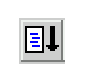
\epsfig{file=Figures/nodebug.eps}}
      beantwortet die gestellte Anfrage ohne weitere Unterbrechung.

      Alternative hat die Taste ``\texttt{n}'' (\emph{nodebug}) dieselbe Funktion.

      Von den weiteren Schaltfl\"{a}chen sind f\"{u}rs erste nur noch zwei interessant.
\item Die Schaltfl\"{a}che \raisebox{-0.2cm}{
\epsfig{file=Figures/continue.eps}}
       l\"{a}sst das Programm bis zum n\"{a}chsten Haltepunkt laufen.

      Alternative hat die Taste ``\texttt{l}'' (\emph{continue}) dieselbe Funktion.
\item Die Schaltfl\"{a}che \raisebox{-0.2cm}{
\epsfig{file=Figures/break.eps}} 
      setzt einen Haltepunkt.  Dazu muss vorher der Cursor an die Stelle gebracht
      werden, an der ein Haltepunkt gesetzt werden soll.

      Alternative hat die Taste ``\texttt{!}''  dieselbe Funktion.
\end{enumerate}

\begin{figure}[!h]
  \centering
  \framebox{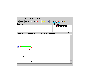
\epsfig{file=Figures/debug.eps,scale=0.7}} 
  \caption{Der Debugger des \textsl{SWI-Prolog}-Systems.}
  \label{fig:debugger}
\end{figure}

Wir zeigen, wie das Ziel \texttt{maechtig(X), spinnt(X)} 
vom \textsl{Prolog}-System beantwortet wird.  
\begin{enumerate}
\item Zun\"{a}chst wird versucht, die Anfrage ``\texttt{maechtig(X)}'' zu l\"{o}sen.
      Die erste Regel, die das Pr\"{a}dikat \texttt{maechtig/1} definiert,
      ist \\[0.2cm]
      \hspace*{1.3cm} \texttt{maechtig(X) :- stark(X).}\\[0.2cm]
      Daher wird die Anfrage ``\texttt{maechtig(X)}'' reduziert zu der Anfrage 
      ``\texttt{stark(X)}''.  Die aktuelle vollst\"{a}ndige Anfrage lautet nun \\[0.2cm]
      \hspace*{1.3cm} \texttt{stark(X), spinnt(X)}. \\[0.2cm]
      Da es noch eine zweite Regel gibt, die das Pr\"{a}dikat \texttt{maechtig/1} definiert,
      setzen wir an dieser Stelle einen Auswahl-Punkt (\emph{Choice-Point}).  Falls also die 
      Beantwortung der Anfrage ``\texttt{stark(X), spinnt(X)}'' sp\"{a}ter scheitert,
      k\"{o}nnen wir es mit der zweiten Regel noch einmal versuchen.
\item Jetzt wird versucht, die Anfrage ``\texttt{stark(X)}'' zu l\"{o}sen.
      Die erste und einzige Regel, die das Pr\"{a}dikat \texttt{stark/1} definiert, ist 
      \\[0.2cm]
      \hspace*{1.3cm} \texttt{stark(X) :- gallier(X).} \\[0.2cm]
      Nach der Unifikation des Kopfes dieser Regel mit der Anfrage ``\texttt{stark(X)}''
      lautet die aktuelle Anfrage \\[0.2cm]
      \hspace*{1.3cm} 
      \texttt{gallier(X), spinnt(X).}
\item Die erste Regel, die das Pr\"{a}dikat \texttt{gallier/1} definiert und deren Kopf
      mit der Anfrage ``\texttt{gallier(X)}'' unifiziert werden kann, ist der Fakt \\[0.2cm]
      \hspace*{1.3cm} \texttt{gallier(asterix).} \\[0.2cm]
      Bei der Unifikation mit diesem Fakt wird die Variable \texttt{X} an die Konstante
      \texttt{asterix} gebunden.  Damit lautet jetzt die aktuelle Anfrage \\[0.2cm]
      \hspace*{1.3cm} 
      \texttt{spinnt(asterix).} \\[0.2cm]
      Da es noch eine zweite Regel gibt, die das Pr\"{a}dikat \texttt{gallier/1} definiert,
      setzen wir an dieser Stelle einen Auswahl-Punkt.   
\item Die erste und einzige Regel, die das Pr\"{a}dikat \texttt{spinnt/1} definiert,
      lautet \\[0.2cm]
      \hspace*{1.3cm} 
      \texttt{spinnt(X) :- roemer(X).} \\[0.2cm]
      Also wird nun die Variable \texttt{X} in dieser Regel mit \texttt{asterix} 
      unifiziert und wir erhalten die Anfrage \\[0.2cm]
      \hspace*{1.3cm} 
      \texttt{roemer(asterix).}
\item Die einzige Regel, die das Pr\"{a}dikat \texttt{roemer/1} definiert, ist \\[0.2cm]
      \hspace*{1.3cm} 
      \texttt{roemer(caesar).} \\[0.2cm]
      Diese Regel l\"{a}sst sich nicht mit der Anfrage ``\texttt{roemer(asterix)}'' unifizieren.
      Also scheitert diese Anfrage.
\item Wir schauen nun, wann wir das letzte mal einen Auswahl-Punkt gesetzt haben.
      Wir stellen fest, dass wir unter Punkt 3 bei der Beantwortung der Anfrage
      \texttt{gallier(X)} das letzte Mal einen Auswahl-Punkt gesetzt haben.
      Also gehen wir nun zu Punkt 3 zur\"{u}ck und versuchen wieder, die Anfrage
      \\[0.2cm]
      \hspace*{1.3cm} 
      \texttt{gallier(X), spinnt(X)} \\[0.2cm]
      zu l\"{o}sen.  Diesmal w\"{a}hlen wir jedoch den Fakt \\[0.2cm]
      \hspace*{1.3cm} \texttt{gallier(obelix).}  \\[0.2cm]
      Wir erhalten dann die neue Anfrage \\[0.2cm]
      \hspace*{1.3cm} \texttt{spinnt(obelix).}
\item Die erste und einzige Regel, die das Pr\"{a}dikat \texttt{spinnt/1} definiert,
      lautet \\[0.2cm]
      \hspace*{1.3cm} 
      \texttt{spinnt(X) :- roemer(X).} \\[0.2cm]
      Also wird die Variable \texttt{X} in dieser Regel mit \texttt{obelix} 
      unifiziert und wir erhalten die Anfrage \\[0.2cm]
      \hspace*{1.3cm} 
      \texttt{roemer(obelix).}
\item Die einzige Regel, die das Pr\"{a}dikat \texttt{roemer/1} definiert, ist \\[0.2cm]
      \hspace*{1.3cm} 
      \texttt{roemer(caesar).} \\[0.2cm]
      Diese Regel l\"{a}sst sich nicht mit der Anfrage ``\texttt{roemer(asterix)}'' unifizieren.
      Also scheitert diese Anfrage.
\item Wir schauen wieder, wann das letzte Mal ein Auswahl-Punkt gesetzt wurde.
      Der unter Punkt 3~gesetzte Auswahl-Punkt wurde vollst\"{a}ndig abgearbeitet, dieser
      Auswahl-Punkt kann uns also nicht mehr helfen.
      Aber unter Punkt 1 wurde ebenfalls ein Auswahl-Punkt gesetzt, denn f\"{u}r das Pr\"{a}dikat
      \texttt{maechtig/1} gibt es die weitere Regel \\[0.2cm]
      \hspace*{1.3cm} \texttt{maechtig(X) :- kaiser(X), roemer(X)}. \\[0.2cm]
      Wenden wir diese Regel an, so erhalten wir die Anfrage \\[0.2cm]
      \hspace*{1.3cm} 
      \texttt{kaiser(X), roemer(X), spinnt(X).}
\item F\"{u}r das Pr\"{a}dikat \texttt{kaiser/1} enth\"{a}lt unsere Datenbank genau einen Fakt:\\[0.2cm]
      \hspace*{1.3cm} \texttt{kaiser(caesar).}  \\[0.2cm]
      Benutzen wir diesen Fakt zur Reduktion unserer Anfrage, so  lautet die neue Anfrage \\[0.2cm]
      \hspace*{1.3cm} 
      \texttt{roemer(caesar), spinnt(caesar).}
\item F\"{u}r das Pr\"{a}dikat \texttt{roemer/1} enth\"{a}lt unsere Datenbank genau einen Fakt:\\[0.2cm]
      \hspace*{1.3cm} \texttt{roemer(caesar).}  \\[0.2cm]
      Benutzen wir diesen Fakt zur Reduktion unserer Anfrage, so  lautet die neue Anfrage \\[0.2cm]
      \hspace*{1.3cm} 
      \texttt{spinnt(caesar).}
\item Die erste und einzige Regel, die das Pr\"{a}dikat \texttt{spinnt/1} definiert,
      lautet \\[0.2cm]
      \hspace*{1.3cm} 
      \texttt{spinnt(X) :- roemer(X).} \\[0.2cm]
      Also wird die Variable \texttt{X} in dieser Regel mit \texttt{caesar} 
      unifiziert und wir erhalten die Anfrage \\[0.2cm]
      \hspace*{1.3cm} 
      \texttt{roemer(caesar).}
\item F\"{u}r das Pr\"{a}dikat \texttt{roemer/1} enth\"{a}lt unsere Datenbank genau einen Fakt:\\[0.2cm]
      \hspace*{1.3cm} \texttt{roemer(caesar).}  \\[0.2cm]
      Benutzen wir diesen Fakt zur Reduktion unserer Anfrage, so ist die verbleibende
      Anfrage leer.  Damit ist die urspr\"{u}ngliche Anfrage gel\"{o}st.  Die dabei berechnete
      Antwort erhalten wir, wenn wir untersuchen, wie die Variable \texttt{X} unifiziert
      worden ist.  Die Variable \texttt{X} war unter Punkt 10 mit der Konstanten
      \texttt{caesar} unifiziert worden.  Also ist \\[0.2cm]
      \hspace*{1.3cm} \texttt{X = caesar}
      \\[0.2cm]
      die Antwort, die von dem System berechnet wird.
\end{enumerate}
Bei der Beantwortung der Anfrage ``\texttt{maechtig(X), spinnt(X)}'' sind wir einige Male
in Sackgassen hineingelaufen und mussten Instantiierungen der Variable \texttt{X} wieder
zur\"{u}ck nehmen.  Dieser Vorgang wird in der Literatur als \emph{backtracking} bezeichnet.
Er kann mit Hilfe des Debuggers am Bildschirm verfolgt werden.

\subsection{Die Tiefensuche}
Der von Prolog verwendete Such-Algorithmus wird auch als \emph{Tiefensuche} (angels\"{a}chsisch:
\emph{depth first search}) bezeichnet.  Um diesen Ausdruck erl\"{a}utern zu k\"{o}nnen, definieren wir
zun\"{a}chst den Begriff des \emph{Suchbaums}.  Die Knoten eines Suchbaums sind mit Anfrage beschriftet.
Ist der Knoten $u$ des Suchbaums mit der Anfrage
\[ Q_1, \cdots, Q_m \]
beschriftet und gibt es f\"{u}r $i = 1,\cdots,k$ Regeln der Form
\[ A^{(i)} \texttt{:-} B_1^{(i)}, \cdots, B_{n(i)}^{(i)} \]
die auf die Anfrage passen, f\"{u}r die also $\mu_i = \textsl{mgu}(Q_1, A^{(i)})$ existiert, so hat der
Knoten $u$ insgesamt $k$ verschiedene Kinder.  Dabei ist das $i$-te Kind mit der Anfrage
\[  B_1^{(i)}\mu_i, \cdots, B_{n(i)}^{(i)}\mu_i, Q_2\mu_i, \cdots, Q_m\mu_i \]
beschriftet.  Als einfaches Beispiel betrachten wir das in Abbildung \ref{fig:depth.pl} gezeigte
Programm.  Der Suchbaum f\"{u}r die Anfrage
\[ p(X) \]
ist in Abbildung \ref{fig:depth-first.eps} gezeigt.  Den Knoten, der mit der urspr\"{u}nglichen Anfrage
beschriftet ist, bezeichnen wir als die \emph{Wurzel} des Suchbaums.  Die \emph{L\"{o}sungen} zu der
urspr\"{u}nglichen Anfrage finden wir an den \emph{Bl\"{a}ttern} des Baumes: Wir bezeichnen hier die Knoten
als Bl\"{a}tter, die am weitesten unten stehen.  Suchb\"{a}ume stehen also gewisserma�en auf dem Kopf: Die
Bl\"{a}tter sind unten und die Wurzeln sind oben\footnote{
Daher werden diese Suchb\"{a}ume auch als australische B\"{a}ume bezeichnet.}.

\begin{figure}[!ht]
\centering
\begin{Verbatim}[ frame         = lines, 
                  framesep      = 0.3cm, 
                  labelposition = bottomline,
                  numbers       = left,
                  numbersep     = -0.2cm,
                  xleftmargin   = 0.8cm,
                  xrightmargin  = 0.8cm,
                ]
    p(X) :- q1(X).
    p(X) :- q2(X).
    
    q1(X) :- r1(X). 
    q1(X) :- r2(X). 
    
    q2(X) :- r3(X). 
    q2(X) :- r4(X). 
    
    r1(a).
    r2(b).
    r3(c).
    r4(d).
\end{Verbatim}
\vspace*{-0.3cm}
\caption{Die Tiefensuche in Prolog}
\label{fig:depth.pl}
\end{figure}

\begin{figure}[!ht]
\centering
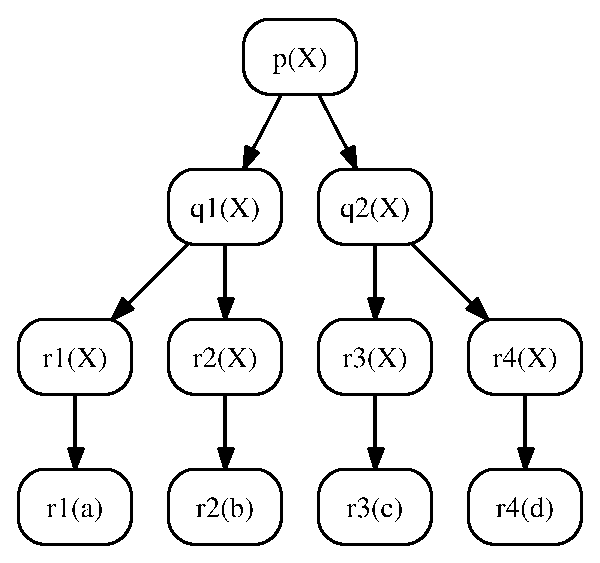
\epsfig{file=depth-first.eps,scale=0.6}

\vspace*{-0.3cm}
\caption{Der Suchbaum f\"{u}r das in Abbildung \ref{fig:depth.pl} gezeigte Programm.}
\label{fig:depth-first.eps}
\end{figure}

Anhand des in Abbildung \ref{fig:depth-first.eps} gezeigten Suchbaums l\"{a}sst sich nun die Tiefensuche
erkl\"{a}ren:  Wenn der Prolog-Interpreter nach einer L\"{o}sung sucht, so w\"{a}hlt er immer den linkesten Ast
und steigt dort so tief wie m\"{o}glich ab.  Dadurch werden die L\"{o}sungen in dem Beispiel in der
Reihenfolge
\[ X = a,\; X = b,\; X = c,\; X = d,\; \]
gefunden.  Die Tiefensuche ist dann problematisch, wenn der linkeste Ast des Suchbaums unendlich
tief ist.  Als Beispiel betrachten wir das  in Abbildung \ref{fig:infinite.pl} gezeigte Prolog-Programm.
Zeichnen wir hier den Suchbaum f\"{u}r die Anfrage
\[ p(X) \]
 so finden wir einen unendlichen Ast, in den der Prolog-Interpreter
absteigt und aus dem er dann mit einem Stack-Overflow wieder zur\"{u}ck kommt.  Vertauschen wir hingegen
die Reihenfolge der Klauseln, so kann das Programm die obige Anfrage beantworten.

\begin{figure}[!ht]
\centering
\begin{Verbatim}[ frame         = lines, 
                  framesep      = 0.3cm, 
                  labelposition = bottomline,
                  numbers       = left,
                  numbersep     = -0.2cm,
                  xleftmargin   = 0.8cm,
                  xrightmargin  = 0.8cm,
                ]
    p(s(X)) :- p(X).
    p(c).
\end{Verbatim}
\vspace*{-0.3cm}
\caption{Eine Endlos-Schleife in \textsl{Prolog}.}
\label{fig:infinite.pl}
\end{figure}

\section{Ein komplexeres Beispiel}
Das obige Beispiel war bewusst einfach gehalten um die Sprache \textsl{Prolog} einzuf\"{u}hren.
Um die M\"{a}chtigkeit des Backtrackings zu demonstrieren, pr\"{a}sentieren wir jetzt ein
komplexeres Beispiel.  Es handelt sich um das folgende R\"{a}tsel:
\begin{enumerate}
\item Drei Freunde belegen den ersten, zweiten und dritten Platz bei einem
      Programmier-Wettbewerb.
\item Jeder der drei hat genau einen Vornamen, genau ein Auto und hat sein Programm
      in genau einer Programmier-Sprache geschrieben.
\item Michael programmiert in \textsc{SetlX} und war besser als der Audi-Fahrer.
\item Julia, die einen Ford Mustang f\"{a}hrt, war besser als der Java-Programmierer.
\item Das Prolog-Programm war am besten.
\item Wer f\"{a}hrt Toyota?
\item In welcher Sprache programmiert Thomas?
\end{enumerate}
Um dieses R\"{a}tsel zu l\"{o}sen, \"{u}berlegen wir uns zun\"{a}chst, wie wir die einzelnen Daten
repr\"{a}sentieren k\"{o}nnen, die in dem R\"{a}tsel eine Rolle spielen.  Zun\"{a}chst ist dort von
Personen die Rede. Jede dieser Personen hat genau einen Vornamen, ein Auto und eine
Programmier-Sprache.   Wir repr\"{a}sentieren Personen daher durch Terme der Form \\[0.2cm]
\hspace*{1.3cm} \texttt{person}(\textsl{Name}, \textsl{Car}, \textsl{Language}). \\[0.2cm]
Dabei bezeichnen \textsl{Name}, \textsl{Car} und \textsl{Language} Konstanten, die aus den
entsprechenden Mengen gew\"{a}hlt werden:
\\[0.2cm]
\hspace*{1.3cm} 
$\textsl{Name} \in \{ \texttt{julia}, \texttt{thomas}, \texttt{michael} \}$, \quad
$\textsl{Car} \in \{ \texttt{ford}, \texttt{toyota}, \texttt{audi} \}$, \\[0.2cm]
\hspace*{1.3cm} 
$\textsl{Language} \in \{ \texttt{java}, \texttt{prolog}, \texttt{setlX} \}$. \\[0.2cm]
Wenn wir Personen durch ein dreistelliges Funktions-Zeichen wie oben gezeigt repr\"{a}sentieren, k\"{o}nnen
wir sofort Pr\"{a}dikate angeben, 
die den Vornamen, die Auto-Marke und die Programmier-Sprache aus einem solchen Term
extrahieren.
\begin{enumerate}
\item Das Pr\"{a}dikat \texttt{first\_name/2} extrahiert den Vornamen: \\[0.2cm]
      \hspace*{1.3cm} \texttt{first\_name(person(Name, Car, Language), Name).}
\item Das Pr\"{a}dikat \texttt{car/2} extrahiert die Auto-Marke: \\[0.2cm]
      \hspace*{1.3cm} \texttt{car(person(Name, Car, Language), Car).}
\item Das Pr\"{a}dikat \texttt{language/2} extrahiert die Programmier-Sprache: \\[0.2cm]
      \hspace*{1.3cm} \texttt{language(person(Name, Car, Language), Language).}
\end{enumerate}
Um zu verstehen wie diese Pr\"{a}dikate arbeiten, zeigen wir, wie die Anfrage \\[0.2cm]
\hspace*{1.3cm} \texttt{car( person(hans, seat, setlX), X ).}\\[0.2cm]
von dem \textsl{Prolog}-System beantwortet wird.  Die einzige Regel, die zur Beantwortung
dieser Anfrage herangezogen werden kann, ist die Regel \\[0.2cm]
\hspace*{1.3cm} \texttt{car(person(Name, Car, Language), Car) :- true.} \\[0.2cm]
Um diese Regel anwenden zu k\"{o}nnen, ist die syntaktische Gleichung \\[0.2cm]
\hspace*{1.3cm} 
$\texttt{car( person(hans, seat, setlX), X )} \doteq \texttt{car( person(Name, Car, Language), Car )}$
\\[0.2cm]
zu l\"{o}sen.  Bei der Unifikation findet sich die L\"{o}sung \\[0.2cm]
\hspace*{1.3cm} 
$\mu = [ \texttt{Name} \mapsto \texttt{hans},\; \texttt{Car} \mapsto \texttt{seat},\;\texttt{Language} \mapsto \texttt{setlX},\; \texttt{X} \mapsto \texttt{seat}]$.
\\[0.2cm]
Insbesondere wird also die Variable \texttt{X} bei dieser Anfrage an die Konstante
\texttt{seat} gebunden.

Wie k\"{o}nnen wir nun die Reihenfolge repr\"{a}sentieren, in der die drei Personen bei dem 
Wettbewerb abgeschnitten haben?  Wir w\"{a}hlen ein dreistelliges Funktions-Zeichen
\texttt{sequence} und repr\"{a}sentieren die Reihenfolge durch den Term
\\[0.2cm]
\hspace*{1.3cm} \texttt{sequence}(\textsl{First}, \textsl{Second}, \textsl{Third}).\\[0.2cm]
Dabei stehen \textsl{First}, \textsl{Second} und \textsl{Third} f\"{u}r Terme, die von dem
Funktions-Zeichen \texttt{person/3} erzeugt worden sind und die Personen bezeichnen.
Die Reihenfolge kann dann durch das Pr\"{a}dikat \\[0.2cm]
\hspace*{1.3cm} \texttt{did\_better}(\textsl{Better}, \textsl{Worse}, \textsl{Sequence})
\\[0.2cm]
berechnet werden, dessen Implementierung in den Zeilen 38 -- 40 der Abbildung
\ref{fig:toyota} auf Seite \pageref{fig:toyota} gezeigt ist.
Wir k\"{o}nnen nun daran gehen, das R\"{a}tsel zu l\"{o}sen.  Abbildung
\ref{fig:toyota} zeigt die Implementierung.
Zeile 1 -- 30 enth\"{a}lt die Implementierung einer Regel f\"{u}r das
Pr\"{a}dikat \texttt{answer/2}, dass die L\"{o}sung des R\"{a}tsel berechnet.  
In dieser Regel haben wir das R\"{a}tsel als pr\"{a}dikatenlogische Formel
codiert.  Wir \"{u}bersetzen diese  Regel jetzt zur\"{u}ck in die Umgangssprache
und zeigen dadurch,  dass das Pr\"{a}dikat \texttt{answer/2} das R\"{a}tsel
korrekt beschreibt.  Die Nummerierung in der folgenden Aufz\"{a}hlung
stimmt jeweils mit der entsprechenden Zeilen-Nummer im Programm \"{u}berein:
\begin{enumerate}
\item[2.] Falls \texttt{Sequence} eine Reihenfolge von drei Personen beschreibt  und
\item[4.] \texttt{Michael} eine Person aus dieser Reihenfolge ist und
\item[5.] der Name der durch \texttt{Michael} bezeichneten Person den Wert \texttt{michael}
         hat und
\item[6.] \texttt{Michael} in \textsc{SetlX} programmiert und
\item[8.] \texttt{Audi} eine Person aus der Reihenfolge \texttt{Sequence} ist und
\item[9.] \texttt{Michael} beim Wettbewerb besser abgeschnitten hat als die durch \texttt{Audi} bezeichnete Person
\item[10.] die durch \texttt{Audi} bezeichnete Person einen Audi f\"{a}hrt und 

           $\vdots$

\item[24.] \texttt{Toyota} eine Person aus der Reihenfolge \texttt{Sequence} ist und
\item[25.] die durch \texttt{Toyota} bezeichnete Person einen Toyota f\"{a}hrt und
\item[26.] \texttt{NameToyota} den Vornamen der durch \texttt{Toyota} bezeichneten Person angibt und
\item[28.] \texttt{Thomas} eine Person aus der Reihenfolge \texttt{Sequence} ist und
\item[25.] die durch \texttt{Thomas} bezeichnete Person den Vornamen Thomas hat und
\item[26.] \texttt{LanguageThomas} die Sprache ist, in der die durch \texttt{Thomas}
          bezeichnete Person programmiert,

          dann gilt:

\item[1.] \texttt{NameToyota} ist der Namen des Toyota-Fahrers und
         \texttt{LanguageThomas} ist die Sprache, in der Thomas programmiert.
\end{enumerate}


\begin{figure}[!h]
  \centering
\begin{Verbatim}[ frame         = lines, 
                  framesep      = 0.3cm, 
                  labelposition = bottomline,
                  numbers       = left,
                  numbersep     = -0.2cm,
                  xleftmargin   = 0.8cm,
                  xrightmargin  = 0.8cm
                ]
    answer(NameToyota, LanguageThomas) :-
        is_sequence( Sequence ),
        % Michael programmiert in SetlX.
        one_of_them(Michael, Sequence),
        first_name(Michael, michael),  
        language(Michael, setlX),
        % Michael war besser als der Audi-Fahrer                     
        one_of_them(Audi, Sequence),
        did_better(Michael, Audi, Sequence),         
        car(Audi, audi),
        % Julia f\"{a}hrt einen Ford Mustang.
        one_of_them(Julia, Sequence),
        first_name(Julia, julia),
        car(Julia, ford), 
        % Julia war besser als der Java-Programmierer.
        one_of_them(JavaProgrammer, Sequence),
        language(JavaProgrammer, java),
        did_better(Julia, JavaProgrammer, Sequence), 
        % Das Prolog-Programm war am besten.
        one_of_them(PrologProgrammer, Sequence),
        first(PrologProgrammer, Sequence),           
        language(PrologProgrammer, prolog),
        % Wer f\"{a}hrt Toyota?
        one_of_them(Toyota, Sequence),
        car(Toyota, toyota),
        first_name(Toyota, NameToyota),              
        % In welcher Sprache programmiert Thomas?
        one_of_them(Thomas, Sequence),
        first_name(Thomas, thomas),
        language(Thomas, LanguageThomas).            
        
    is_sequence( sequence(_First, _Second, _Third) ).
    
    one_of_them(A, sequence(A, _, _)).
    one_of_them(B, sequence(_, B, _)).
    one_of_them(C, sequence(_, _, C)).
    
    did_better(A, B, sequence(A, B, _)).
    did_better(A, C, sequence(A, _, C)).
    did_better(B, C, sequence(_, B, C)).
    
    first(A, sequence(A, _, _)).
    
    first_name(person(Name, _Car, _Language), Name).
    
    car(person(_Name, Car, _Language), Car).
    
    language(person(_Name, _Car, Language), Language).
\end{Verbatim}
\vspace*{-0.3cm}
  \caption{Wer f\"{a}hrt Toyota?}
  \label{fig:toyota}
\end{figure}

Wenn wir die urspr\"{u}ngliche Aufgabe mit der Implementierung in \textsl{Prolog} vergleichen,
dann stellen wir fest, dass die in dem R\"{a}tsel gemachten Angaben eins-zu-eins in
\textsl{Prolog} \"{u}bersetzt werden konnten.  Diese \"{u}bersetzung beschreibt nur das R\"{a}tsel und
gibt keinen Hinweis, wie dieses R\"{a}tsel zu l\"{o}sen ist.  F\"{u}r die L\"{o}sung ist dann die dem
\textsl{Prolog}-System zu Grunde liegende \textsl{Inferenz-Maschine} zust\"{a}ndig.

\section{Listen}
In Prolog wird viel mit Listen gearbeitet.  Listen werden in Prolog mit dem
2-stelligen Funktions-Zeichen ``\texttt{.}'' konstruiert.  Ein Term der Form \\[0.2cm]
\hspace*{1.3cm} \texttt{.($s$,$t$)} \\[0.2cm]
steht also f\"{u}r eine Liste, die als erstes Element ``$s$'' enth\"{a}lt. ``$t$'' bezeichnet den
Rest der Liste.
Das Funktions-Zeichen ``\texttt{[]}'' steht
f\"{u}r die leere Liste. Eine Liste, die aus  den drei Elementen 
``\texttt{a}'', ``\texttt{b}'' und ``\texttt{c}'' besteht, kann also wie folgt dargestellt
werden: \\[0.2cm]
\hspace*{1.3cm} \texttt{.(a, .(b, .(c, [])))} \\[0.2cm]
Da dies relativ schwer zu lesen ist, darf diese Liste auch als \\[0.2cm]
\hspace*{1.3cm} \texttt{[a,b,c]} \\[0.2cm]
geschrieben werden.  Zus\"{a}tzlich kann der Term ``\texttt{.($s$,$t$)}'' in der Form \\[0.2cm]
\hspace*{1.3cm} \texttt{[ $s$ | $t$ ]} \\[0.2cm]
geschrieben werden.  Um diese Kurzschreibweise zu erl\"{a}utern, geben wir ein kurzes
Prolog-Programm an, das zwei Listen aneinander h\"{a}ngen kann.  
Das Programm implementiert das dreistellige Pr\"{a}dikat \texttt{myAppend}\footnote{In dem
  \textsl{SWI-Prolog}-System gibt es das vordefinierte Pr\"{a}dikat \texttt{append/3},
  das genau dasselbe leistet wie unsere Implementierung von \texttt{myAppend/3}.}.  
Die Intention ist,
dass $\texttt{myAppend}(l_1,l_2,l_3)$ f\"{u}r drei Listen $l_1$, $l_2$ und $l_3$ genau dann
wahr sein soll,
wenn die Liste $l_3$ dadurch entsteht, dass die Liste $l_2$ hinten an die Liste $l_1$
angeh\"{a}ngt wird.  Das Programm besteht aus den folgenden beiden Klauseln:
\begin{verbatim}
  myAppend( [], L, L ).
  myAppend( [ X | L1 ], L2, [ X | L3 ] ) :- myAppend( L1, L2, L3 ).
\end{verbatim}
Wir k\"{o}nnen diese beiden Klauseln folgenderma�en in die Umgangssprache \"{u}bersetzen:
\begin{enumerate}
\item H\"{a}ngen wir eine Liste \texttt{L} an die leere Liste an, so ist das Ergebnis die
      Liste \texttt{L}.
\item Um an eine Liste \texttt{[ X | L1 ]}, die aus dem Element \texttt{X} und dem Rest \texttt{L1} besteht,
      eine Liste \texttt{L2} anzuh\"{a}ngen, h\"{a}ngen wir zun\"{a}chst an die Liste \texttt{L1} die 
      Liste \texttt{L2} an und nennen das Ergebnis \texttt{L3}.  
      Das Endergebnis erhalten wir, wenn wir vor die Liste \texttt{L3} noch das Element \texttt{X}
      setzen.  Wir erhalten dann die Liste \texttt{[ X | L3 ]}.
\end{enumerate}
Wir testen unser Programm und nehmen dazu an, dass die beiden Programm-Klauseln in der Datei
``\texttt{myAppend.pl}'' abgespeichert sind und dass wir diese Datei mit dem Befehl ``\texttt{consult(myAppend).}'' geladen haben.
Dann stellen wir die Anfrage \\[0.2cm]
\hspace*{1.3cm} \texttt{?- myAppend( [ 1, 2, 3 ], [ a, b, c ], L ).} \\[0.2cm]
Wir erhalten die Antwort:
\begin{verbatim}
    L = [1, 2, 3, a, b, c] 
\end{verbatim}
Die obige Interpretation des gegebenen Prolog-Programms ist \emph{funktional}, dass hei�t 
wir fassen die ersten beiden Argumente des Pr\"{a}dikats \texttt{myAppend} als \emph{Eingaben} auf und 
interpretieren das letzte Argument als \emph{Ausgabe}.  Diese Interpretation ist aber keineswegs die 
einzig m\"{o}gliche Interpretation.  Um das zu sehen, geben wir als Ziel \\[0.2cm]
\hspace*{1.3cm} \texttt{myAppend(L1, L2, [1,2,3]).} \\[0.2cm]
ein und dr\"{u}cken, nachdem das System uns die erste Antwort gegeben hat, nicht die Taste 
\textsl{Return} sondern die Taste ``\texttt{;}''.  Wir erhalten:
\begin{verbatim}
    ?- myAppend(L1, L2, [1, 2, 3]).

    L1 = []
    L2 = [1, 2, 3] ;

    L1 = [1]
    L2 = [2, 3] ;

    L1 = [1, 2]
    L2 = [3] ;

    L1 = [1, 2, 3]
    L2 = [] ;

    No
\end{verbatim}
In diesem Fall hat das Prolog-System durch Backtracking  alle M\"{o}glichkeiten bestimmt, die
es gibt, um die Liste ``\texttt{[1, 2, 3]}'' in zwei Teillisten zu zerlegen.

\subsection{Sortieren durch Einf\"{u}gen}
Wir entwickeln nun einen einfachen Algorithmus zum Sortieren von Listen von Zahlen.
Die Idee ist Folgende:  Um eine Liste aus $n$ Zahlen zu sortieren, sortieren wir zun\"{a}chst
die letzten $n-1$ Zahlen und f\"{u}gen dann das erste Element an der richtigen Stelle in die sortierte
Liste ein.  Mit dieser Idee besteht das Programm aus zwei Pr\"{a}dikaten:
\begin{enumerate}
\item Das Pr\"{a}dikat \texttt{insert/3} erwartet
      als erstes Argument eine Zahl $x$ und als zweites Argument eine Liste von Zahlen $l$,
      die bereits in aufsteigender Reihenfolge sortiert ist.  
      Das Pr\"{a}dikat f\"{u}gt die Zahl $x$ so in die Liste $l$ ein, dass die resultierende Liste
      ebenfalls in aufsteigender Reihenfolge sortiert ist. Das so berechnete Ergebnis
      wird als letztes Argument des Pr\"{a}dikats \texttt{insert/3} zur\"{u}ck gegeben.  

      Um die obigen Ausf\"{u}hrungen
      \"{u}ber die verwendeten Typen und die Bestimmung von Ein- und Ausgabe pr\"{a}gnanter
      formulieren zu k\"{o}nnen, f\"{u}hren wir den Begriff einer \emph{Typ-Spezifikation} ein.
      F\"{u}r das Pr\"{a}dikat \texttt{insert/3} hat diese Typ-Spezifikation die Form \\[0.2cm]
      \hspace*{1.3cm} 
      \texttt{insert(+\textsl{Number}, +\textsl{List}(\textsl{Number}), -\textsl{List}(\textsl{Number}))}.
      \\[0.2cm]
      Das Zeichen ``\texttt{+}'' legt dabei fest, dass das entsprechende
      Argument eine Eingabe ist, w\"{a}hrend ``\texttt{-}'' verwendet wird um ein
      Ausgabe-Argument zu spezifizieren.
\item Das Pr\"{a}dikat \texttt{insertion\_sort/2} hat die Typ-Spezifikation \\[0.2cm]
      \hspace*{1.3cm} \texttt{insertion\_sort(+\textsl{List}(\textsl{Number}), -\textsl{List}(\textsl{Number}))}.
      \\[0.2cm]
      Der Aufruf \texttt{insertion\_sort}(\textsl{List}, \textsl{Sorted}) sortiert die als Eingabe
      gegebene Liste \textsl{List} in aufsteigender Reihenfolge.
\end{enumerate}


\begin{figure}[!h]
  \centering
\begin{Verbatim}[ frame         = lines, 
                  framesep      = 0.3cm, 
                  labelposition = bottomline,
                  numbers       = left,
                  numbersep     = -0.2cm,
                  xleftmargin   = 0.8cm,
                  xrightmargin  = 0.8cm
                ]
    % insert( +Number, +List(Number), -List(Number) ).

    insert( X, [], [ X ] ). 

    insert( X, [ Head | Tail ], [ X, Head | Tail ] ) :-
        X =< Head.

    insert( X, [ Head | Tail ], [ Head | New_Tail ] ) :-
        X > Head,
        insert( X, Tail, New_Tail ).

    % insertion_sort( +List(Number), -List(Number) ).

    insertion_sort( [], [] ).

    insertion_sort( [ Head | Tail ], Sorted ) :-
        insertion_sort( Tail, Sorted_Tail ),
        insert( Head, Sorted_Tail, Sorted ).
\end{Verbatim}
\vspace*{-0.3cm}
  \caption{Sortieren durch Einf\"{u}gen.}
  \label{fig:insertion-sort}
\end{figure}

Abbildung \ref{fig:insertion-sort} auf Seite \pageref{fig:insertion-sort} zeigt das \textsl{Prolog}-Programm. 
Nachfolgend diskutieren wir die einzelnen Klauseln der Implementierung des Pr\"{a}dikats \texttt{insert}.
\begin{enumerate}
\item Die erste Klausel des Pr\"{a}dikats \texttt{insert} greift, wenn die Liste, in welche die
      Zahl \texttt{X} eingef\"{u}gt werden soll, leer ist.
      In diesem Fall wird als Ergebnis einfach die Liste zur\"{u}ck gegeben, die als einziges Element
      die Zahl \texttt{X} enth\"{a}lt.
\item Die zweite Klausel greift, wenn die Liste, in die die Zahl  \texttt{X} eingef\"{u}gt
      werden soll, nicht leer ist und wenn au�erdem
       \texttt{X} kleiner oder gleich dem ersten Element dieser Liste ist.  In diesem Fall kann \texttt{X} an den Anfang der 
      Liste gestellt werden. Dann erhalten wir die Liste \\[0.2cm]
      \hspace*{1.3cm} \texttt{[ X, Head | Tail ]}. \\[0.2cm]
      Diese Liste ist sortiert, weil einerseits schon die Liste \texttt{[ Head | Tail ]} sortiert ist
      und andererseits \texttt{X} kleiner als \texttt{Head} ist.
\item Die dritte Klausel greift, wenn die Liste, in die die Zahl  \texttt{X} eingef\"{u}gt
      werden soll  nicht leer ist und wenn au�erdem \texttt{X} gr\"{o}�er als das erste
      Element dieser Liste ist.  In diesem Fall muss \texttt{X} rekursiv
      in die Liste \texttt{Tail} eingef\"{u}gt werden.  Dabei bezeichnet \texttt{Tail} den
      Rest der Liste, in die wir \texttt{X} einf\"{u}gen wollen.
      Weiter bezeichnet \texttt{New\_Tail} die Liste, die wir erhalten, wenn wir die Zahl
      \texttt{X} in die Liste \texttt{Tail} einf\"{u}gen.
      An den Anfang der  Liste \texttt{New\_Tail} setzen wir nun noch den Kopf
      \texttt{Head} der als Eingabe gegebenen Liste.
\end{enumerate}
Damit k\"{o}nnen wir nun auch die Wirkungsweise des Pr\"{a}dikats \texttt{insertion\_sort} erkl\"{a}ren.
\begin{enumerate}
\item Ist die zu sortierende Liste leer, so ist das Ergebnis die leere Liste.
\item Ist die zu sortierende Liste nicht leer und hat die Form \texttt{[Head | Tail]}, so sortieren wir zun\"{a}chst die
      Liste \texttt{Tail} und erhalten als Ergebnis die sortierte Liste \texttt{Sorted\_Tail}.  F\"{u}gen wir hier
      noch das Element \texttt{Head} mit Hilfe von \texttt{insert} ein, so erhalten wir als Endergebnis
      die sortierte Liste.
\end{enumerate}
Viele \textsl{Prolog}-Pr\"{a}dikate sind \emph{funktional}.  
Wir nennen ein Pr\"{a}dikat funktional,
wenn die einzelnen Argumente klar in Eingabe- und Ausgabe-Argumente unterschieden werden
k\"{o}nnen und wenn au�erdem zu jeder Eingabe h\"{o}chstens eine Ausgabe berechnet wird.
Zum Beispiel sind die oben angegebenen Pr\"{a}dikate zum Sortieren einer Liste von Zahlen funktional.
Bei einem funktionalen Programm k\"{o}nnen wir die Semantik oft dadurch am besten verstehen,
dass wir das Programm in \emph{bedingte Gleichungen} umformen.  F\"{u}r das oben angegebene
Programm erhalten wir dann die folgenden Gleichungen:
\begin{enumerate}
\item $\texttt{insert}( \textsl{X}, []) = [ \textsl{X} ]$. 
\item $\textsl{X} \leq \texttt{\textsl{Head}} \rightarrow \texttt{insert}(\textsl{X}, [ \textsl{Head} | \textsl{Tail} ]) =  [ \textsl{X}, \textsl{Head} | \textsl{Tail} ]$.
\item $\textsl{X} > \texttt{\textsl{Head}} \rightarrow \texttt{insert}(\textsl{X}, [ \textsl{Head} | \textsl{Tail} ]) =  [ \textsl{Head} | \texttt{insert}(\textsl{X}, \textsl{Tail}) ]$.
\item $\texttt{insertion\_sort}([]) = []$.
\item $\texttt{insertion\_sort}([ \textsl{Head} | \textsl{Tail} ]) = \texttt{insert}(\textsl{Head}, \texttt{insertion\_sort}(\textsl{Tail}))$.
\end{enumerate}
Die Korrespondenz zwischen dem \textsl{Prolog}-Programm und den Gleichungen sollte
augenf\"{a}llig sein.  Au�erdem ist offensichtlich, dass die obigen Gleichungen 
den Sortier-Algorithmus in sehr pr\"{a}gnanter Form wiedergeben.  Wir werden diese Beobachtung
im zweiten Semester benutzen und die meisten dort vorgestellten Algorithmen durch bedingte
Gleichungen spezifizieren. 

\subsection{Sortieren durch Mischen}
Der im letzten Abschnitt vorgestellte Sortier-Algorithmus hat einen Nachteil:  Die Rechenzeit,
die dieser Algorithmus verbraucht, w\"{a}chst im ung\"{u}nstigsten Fall quadratisch mit der L\"{a}nge der zu sortierenden 
Liste.  Den Beweis dieser Behauptung werden wir im n\"{a}chsten Semester liefern.
Wir werden nun einen Algorithmus vorstellen der effizienter ist:  Ist $n$ die L\"{a}nge der
Liste, so w\"{a}chst bei diesem Algorithmus der Verbrauch der 
Rechenzeit nur mit dem Faktor $n \cdot \textsl{log}_2(n)$.  Den Nachweis dieser Behauptung
erbringen wir im zweiten Semester.
Wenn es sich bei der zu sortierenden Liste beispielsweise um ein Telefonbuch mit einer
Millionen Eintr\"{a}gen handelt, dann ist der relative Unterschied zwischen $n^2$ und $n \log_2(n)$ bei
etwa $50\,000$. 

Wir werden den effizienteren Algorithmus zun\"{a}chst durch bedingte Gleichungen beschreiben und
anschlie�end die Umsetzung dieser Gleichungen in \textsl{Prolog} angeben.
Der Algorithmus wird in der Literatur als \emph{Sortieren durch Mischen} bezeichnet
(engl. \emph{merge sort}) und besteht aus drei Phasen:
\begin{enumerate}
\item In der ersten Phase wird die zu sortierende Liste in zwei etwa gleich gro�e
      Teillisten aufgeteilt.
\item In der zweiten Phase werden diese Teillisten rekursiv sortiert.
\item In der dritten Phase werden die sortierten Teillisten so zusammen gef\"{u}gt (gemischt),
      dass die resultierende Liste ebenfalls sortiert ist.
\end{enumerate}

Wir beginnen mit dem Aufteilen einer Liste in zwei Teile.  Bei der Aufteilung orientieren wir
uns an den Indizes der Elemente.  Zur Illustration zun\"{a}chst ein Beispiel: Wir teilen die Liste \\[0.2cm]
\hspace*{1.3cm} 
$[a_1, a_2, a_3, a_4, a_5, a_6, a_7, a_8]$ \quad auf in \quad
$[a_1, a_3, a_5, a_7]$ \quad und \quad $[a_2, a_4, a_6, a_8]$.
\\[0.2cm]
Elemente, deren Index gerade ist, werden in der ersten
Teilliste aufgesammelt und die Elemente mit ungeradem Index sammeln wir in der zweiten
Teilliste.  Als Namen f\"{u}r die  Funktionen, die diese Teillisten berechnen, w\"{a}hlen 
wir \texttt{even} und \texttt{odd}: \\[0.2cm]
\hspace*{1.3cm} 
$\texttt{odd}: \textsl{List}(\textsl{Number}) \rightarrow \textsl{List}(\textsl{Number})$,
\\[0.2cm]
\hspace*{1.3cm} 
$\texttt{even}: \textsl{List}(\textsl{Number}) \rightarrow \textsl{List}(\textsl{Number})$.
\\[0.2cm]
Die Funktion $\texttt{odd}(L)$ berechnet die Liste aller Elemente aus $L$ mit ungeradem Index, 
w\"{a}hrend $\mathtt{even}(L)$ die Liste aller Elemente mit geradem Index berechnet.
Die beiden Funktionen k\"{o}nnen durch die folgenden Gleichungen spezifiziert werden:
\begin{enumerate}
\item $\texttt{odd}([]) = []$.
\item $\texttt{odd}([h|t]) = [h|\texttt{even}(t)]$,

      denn das erste Element einer Liste hat den Index 1, was offenbar ein ungerader Index
      ist und alle Elemente, die in der Liste $t$ einen geraden Index haben, haben in der
      Liste $[h|t]$ einen ungeraden Index.
\item $\texttt{even}([]) = []$.
\item $\texttt{even}([h|t]) = \texttt{odd}(t)$,

      denn alle Elemente, die in der Liste $t$ einen ungeraden Index haben, haben in der Liste
      $[h|t]$ einen geraden Index.
\end{enumerate}
Als n\"{a}chstes entwickeln wir eine Funktion \\[0.2cm]
\hspace*{1.3cm} $\texttt{mix}: \textsl{List}(\textsl{Number}) \times \textsl{List}(\textsl{Number}) \rightarrow \textsl{List}(\textsl{Number})$
\\[0.2cm]
die zwei aufsteigend sortierte Listen so mischt,  dass die resultierende Liste ebenfalls
aufsteigend sortiert ist.  Durch rekursive Gleichungen kann diese Funktion wie folgt
spezifiziert werden: 
\begin{enumerate}
\item $\texttt{mix}([], l) = l$.
\item $\texttt{mix}(l, []) = l$.
\item $x \leq y \rightarrow \texttt{mix}([x|s], [y|t]) = [x|\texttt{mix}(s, [y|t])]$.

      Falls $x \leq y$ ist, so ist $x$ sicher das kleinste Element
      der Liste, die entsteht, wenn wir die bereits sortierten Listen $[x|s]$ und $[y|t]$ mischen.
      Also mischen wir rekursiv die Listen $s$ und $[y|t]$ und setzen $x$ an den Anfang
      dieser Liste.
\item $x  >   y \rightarrow \texttt{mix}([x|s], [y|t]) = [y|\texttt{mix}([x|s], t)]$.
\end{enumerate}
Damit k\"{o}nnen wir jetzt die Funktion\\[0.2cm]
\hspace*{1.3cm}  $\texttt{merge\_sort}: \textsl{List}(\textsl{Number}) \rightarrow \textsl{List}(\textsl{Number})$,
\\[0.2cm]
die eine Liste von Zahlen sortiert, durch bedingte Gleichungen spezifizieren.
\begin{enumerate}
\item $\texttt{merge\_sort}([]) = []$.
\item $\texttt{merge\_sort}([x]) = [x]$.
\item $\mathtt{length}(l) \geq 2 \rightarrow \texttt{merge\_sort}(l) = \texttt{mix}(
  \texttt{merge\_sort}(\texttt{odd}(l)),
  \texttt{merge\_sort}(\texttt{even}(l)))$.

      Falls die Liste $l$ aus 2 oder mehr Elementen besteht, teilen wir diese Liste
      in die beiden Listen $\mathtt{odd}(l)$ und $\mathtt{even}(l)$ auf, sortieren 
      diese Listen und mischen anschlie�end die sortierten Teillisten.
\end{enumerate}
Die oben angegebenen Gleichungen lassen sich nun unmittelbar in ein
\textsl{Prolog}-Programm umsetzen.  Abbildung \ref{fig:merge-sort}
auf Seite \pageref{fig:merge-sort} zeigt das resultierende \textsl{Prolog}-Programm.
Da es in \textsl{SWI-Prolog} bereits vordefinierte Pr\"{a}dikate mit den Namen 
\texttt{merge/3} und \texttt{sort/2} gibt, habe ich statt dessen die Namen
\texttt{mix/2} und \texttt{merge\_sort/3} gew\"{a}hlt.


\begin{figure}[!h]
  \centering
\begin{Verbatim}[ frame         = lines, 
                  framesep      = 0.3cm, 
                  labelposition = bottomline,
                  numbers       = left,
                  numbersep     = -0.2cm,
                  xleftmargin   = 0.8cm,
                  xrightmargin  = 0.8cm
                ]
    % odd( +List(Number), -List(Number) ).
    odd( [], [] ).    
    odd( [ X | Xs ], [ X | L ] ) :-
        even( Xs, L ).
    
    % even( +List(Number), -List(Number) ).
    even( [], [] ).
    even( [ _X | Xs ], L ) :-
        odd( Xs, L ).
    
    % merge( +List(Number), +List(Number), -List(Number) ).
    mix( [], Xs, Xs ).    
    mix( Xs, [], Xs ).
    mix( [ X | Xs ], [ Y | Ys ], [ X | Rest ] ) :-
        X =< Y,
        mix( Xs, [ Y | Ys ], Rest ).    
    mix( [ X | Xs ], [ Y | Ys ], [ Y | Rest ] ) :-
        X > Y,
        mix( [ X | Xs ], Ys, Rest ).
    
    % merge_sort( +List(Number), -List(Number) ).    
    merge_sort( [], [] ).
    merge_sort( [ X ], [ X] ).    
    merge_sort( [ X, Y | Rest ], Sorted ) :-
        odd(  [ X, Y | Rest ], Odd  ),
        even( [ X, Y | Rest ], Even ),
        merge_sort( Odd,  Odd_Sorted  ),
        merge_sort( Even, Even_Sorted ),
        mix( Odd_Sorted, Even_Sorted, Sorted ).
\end{Verbatim}
\vspace*{-0.3cm}
  \caption{Sortieren durch Mischen.}
  \label{fig:merge-sort}
\end{figure}


\subsection{Symbolisches Differenzieren}
Die Sprache \textsl{Prolog} wird gerne f\"{u}r Anwendungen benutzt, bei denen symbolische
Rechnungen eine wesentliche Rolle spielen, denn 
symbolische Rechnungen sind in \textsl{Prolog} dadurch, dass die zu
manipulierenden Objekte in der Regel unmittelbar als Prolog-Terme dargestellt werden
k\"{o}nnen, sehr einfach zu implementieren.  Zur Verdeutlichung zeigen wir ein Programm, mit
dem es m\"{o}glich ist, symbolisch zu differenzieren. 
Im Rahmen einer \"{u}bung haben wir ein \textsc{SetlX}-Programm entwickelt, das arithmetische Ausdr\"{u}cke
symbolisch differenziert.  Damals hatten wir davon profitiert, dass die Sprache \textsc{SetlX} Terme
als Datenstruktur zur Verf\"{u}gung stellt.  Da in der Sprache \textsl{Prolog} Terme ebenfalls fest
eingebaut sind, ist es in
\textsl{Prolog} genauso einfach, symbolisch zu differenzieren.

Die Methodik, mit der wir das \textsl{Prolog}-Programm entwickeln, besteht aus zwei
Schritten:
\begin{enumerate}
\item Als erstes legen wir fest, was genau wir unter einem arithmetischen Ausdruck
      verstehen wollen und wie ein solcher Ausdruck in \textsl{Prolog} repr\"{a}sentiert werden soll.  
      Dazu definieren wir die Menge der \textsl{Prolog}-Terme \textsl{Expr}, 
      die einen arithmetischen Ausdruck darstellen.
\item Dann stellen wir bedingte Gleichungen auf, die eine Funktion
      \[ \texttt{diff}: \textsl{Expr} \times \textsl{Var} \rightarrow \textsl{Expr} \]
      beschreiben.  Diese Gleichungen sind nichts anderes als die mathematischen Regeln,
      die Sie in der Schule f\"{u}r das Differenzieren gelernt haben.
\item Im letzten Schritt implementieren wir diese Gleichungen in Prolog.
\end{enumerate}

\paragraph{Induktive Definition der Menge \textsl{Expr}.}
\begin{enumerate}
\item Variablen sind arithmetische Ausdr\"{u}cke.

      Variablen stellen wir durch nullstellige Funktionszeichen dar.
      Nullstellige Funktionszeichen werden in Prolog auch als \emph{Atome} bezeichnet.
      Damit gilt
      \[ c \in \textsl{Expr} \quad \mbox{f\"{u}r jedes \textsl{Prolog}-Atom $c$}. \]
\item Zahlen sind arithmetische Ausdr\"{u}cke.

      Sowohl die ganzen Zahlen als auch die Flie�komma-Zahlen sind Bestandteil der Sprache
      \textsl{Prolog} und k\"{o}nnen damit durch sich selbst dargestelt werden:
      \[ n \in \textsl{Expr} \quad \mbox{f\"{u}r alle $n \in \mathbb{Z}$}, \]
      \[ r \in \textsl{Expr} \quad \mbox{f\"{u}r alle $r \in \mathbb{R}$}. \]
\item Das Negative eines arithmetischen Ausdrucks ist ein arithmetischer Ausdruck.
      In \textsl{Prolog} kann das Negative durch den un\"{a}ren Operator ``\texttt{-}'' dargestellt
      werden, also haben wir
      \[ \texttt{-}\; t \in \textsl{Expr} \quad \mbox{falls $t \in \textsl{Expr}$}. \]
\item Die Summe, die Differenz, das Produkt, und der Quotient zweier arithmetischen
      Ausdr\"{u}cke ist ein arithmetischer Ausdruck. 
      In \textsl{Prolog} k\"{o}nnen Summe, Differenz, Produkt und Quotient respektive
      durch die bin\"{a}ren Operatoren ``\texttt{+}'', ``\texttt{-}'', ``\texttt{*}'' und ``\texttt{/}'' 
      dargestellt werden, also setzen wir
      \[ s \;\texttt{+}\, t \in \textsl{Expr} \quad \mbox{falls $s,t \in \textsl{Expr}$}. \]
      \[ s \;\texttt{-}\; t \in \textsl{Expr} \quad \mbox{falls $s,t \in \textsl{Expr}$}. \]
      \[ s \;\texttt{*}\; t \in \textsl{Expr} \quad \mbox{falls $s,t \in \textsl{Expr}$}. \]
      \[ s \;\texttt{/}\; t \in \textsl{Expr} \quad \mbox{falls $s,t \in \textsl{Expr}$}. \]
\item Die Potenz zweier arithmetischer Ausdr\"{u}cke ist ein arithmetischer Ausdruck.
      In \textsl{Prolog} kann die Potenz durch den bin\"{a}ren Operator ``\texttt{**}'' dargestellt
      werden, also setzen wir
      \[ s \;\texttt{**}\; t \in \textsl{Expr} \quad \mbox{falls $s,t \in \textsl{Expr}$}. \]
\item Bei der Behandlung spezieller Funktionen beschr\"{a}nken wir uns auf die
      Exponential-Funktion und den nat\"{u}rlichen Logarithmus:
      \[ \texttt{exp}(t) \in \textsl{Expr}  \quad \mbox{falls $t \in \textsl{Expr}$}, \]
      \[ \texttt{ln}(t)  \in \textsl{Expr}  \quad \mbox{falls $t \in \textsl{Expr}$}. \]
\end{enumerate}

\paragraph{Aufstellen der bedingten Gleichungen}
Den Wert von $\texttt{diff}(t,x)$ definieren wir nun durch Induktion nach dem Aufbau des
arithmetischen Ausdrucks $t$.
\begin{enumerate}
\item Bei der Ableitung einer Variablen m\"{u}ssen wir unterscheiden,
      ob wir die Variable nach sich selbst oder nach einer anderen Variablen ableiten.
      \begin{enumerate}
      \item Die Ableitung einer Variablen nach sich selbst gibt den Wert 1:
            \[ y = x \rightarrow \bruch{d\,y}{dx} = 1. \]
            Also haben wir 
            \[ y = x \rightarrow \texttt{diff}(y,x) = 1. \]
      \item Die Ableitung einer Variablen $y$ nach einer anderen Variablen $x$ ergibt den Wert 0:
            \[ y \not= x \rightarrow \bruch{d\,y}{dx} = 0 \]
             Also haben wir 
            \[ y \not= x \rightarrow \texttt{diff}(y,x) = 0. \]
      \end{enumerate}
\item Die Ableitung einer Zahl $n$ ergibt 0: 
      \[ \bruch{d\,n}{dx} = 0.  \]
      Damit haben wir
      \[ \texttt{diff}(n, x) = 0. \]
\item Die Ableitung eines Ausdrucks mit negativen Vorzeichen ist durch 
      \[ \bruch{d}{dx}(-f) = - \bruch{d\,f}{dx} \]
      gegeben.  Die rekursive Gleichung lautet 
      \[ \texttt{diff}(-f,x) = - \texttt{diff}(f,x). \]
\item Die Ableitung einer Summe ergibt sich als Summe der Ableitungen der Summanden: 
      \[ \bruch{d}{dx}(f+g) = \bruch{d\,f}{dx} + \bruch{d\,g}{dx} \]
      Als Gleichung schreibt sich dies 
      \[ \texttt{diff}(f + g, x) = \texttt{diff}(f,x) + \texttt{diff}(g,x). \]
\item Die Ableitung einer Differenz ergibt sich als Differenz der Ableitung der Operanden: 
      \[ \bruch{d}{dx}(f-g) = \bruch{d\,f}{dx} - \bruch{d\,g}{dx} \]
      Als Gleichung schreibt sich dies 
      \[ \texttt{diff}(f - g, x) = \texttt{diff}(f,x) - \texttt{diff}(g,x). \]
\item Die Ableitung eines Produktes wird durch die Produkt-Regel beschrieben: 
      \[ \bruch{d}{dx}(f*g) = \bruch{d\,f}{dx}*g + f*\bruch{d\,g}{dx}. \]
      Dies f\"{u}hrt auf die Gleichung 
      \[ \texttt{diff}(f*g,x) = \texttt{diff}(f,x) * g + f * \texttt{diff}(g,x). \]
\item Die Ableitung eines Quotienten wird durch die Quotienten-Regel beschrieben: 
      \[ \bruch{d}{dx}(f/g) = \bruch{\;\displaystyle \rule[-10pt]{0pt}{12pt}
         \bruch{d\,f}{dx}*g - f*\bruch{d\,g}{dx}\;}{\displaystyle \rule{0pt}{10pt}g*g}. \]
      Dies f\"{u}hrt auf die Gleichung 
      \[ \texttt{diff}(f/g,x) = (\texttt{diff}(f,x) * g - f * \texttt{diff}(g,x)) / (g*g). \]
\item Zur Ableitung eines Ausdrucks der Form $f \,\mathtt{**}\, g$ verwenden wir die folgende Gleichung:
      \\[0.2cm]
      \hspace*{1.3cm}      
      $f \,\mathtt{**}\, g = \texttt{exp}(g*\texttt{ln}(f))$.
      \\[0.2cm]
      Das f\"{u}hrt auf die Gleichung 
      \[ 
         \texttt{diff}(f \;\texttt{**}\; g, x) = 
         \texttt{diff}(\mathtt{exp}(g * \mathtt{ln}(f)), x). 
      \]
\item Bei der Ableitung der Exponential-Funktion ben\"{o}tigen wir die Ketten-Regel:
      \[ \bruch{d}{dx}\textsl{exp}(f) = \bruch{d\,f}{dx}* \textsl{exp}(f). \]
      Das f\"{u}hrt auf die Gleichung 
      \[ \texttt{diff}(\texttt{exp}(f), x) = \texttt{diff}(f,x) * \texttt{exp}(f). \]
\item F\"{u}r die Ableitung des nat\"{u}rlichen Logarithmus finden wir unter Ber\"{u}cksichtigung der Ketten-Regel
      \[ \bruch{d}{dx}\textsl{ln}(f) = \bruch{1}{f}*\bruch{d\,f}{dx}. \]
      Das f\"{u}hrt auf die Gleichung 
      \[ \texttt{diff}(\texttt{exp}(f), x) = \texttt{diff}(f,x)/f. \]
\end{enumerate}

\paragraph{Implementierung in \textsl{Prolog}}
Abbildung \ref{fig:symbolisch-diff} zeigt die Implementierung in \textsl{Prolog}.
An Stelle der zweistelligen Funktion $\textsl{diff}()$ haben wir nun ein dreistelliges Pr\"{a}dikat 
\texttt{diff/3}, dessen letztes Argument das Ergebnis berechnet.
Wir diskutieren die einzelnen Klauseln.
\begin{enumerate}
\item Die beiden Klauseln in den Zeilen 3 -- 9 zeigen, wie eine Variable differenziert werden kann.
      Das Pr\"{a}dikat $\texttt{atom}(X)$ pr\"{u}ft, ob $X$ ein nullstelliges Funktions-Zeichen ist.
      Solche Funktions-Zeichen werden im \textsl{Prolog}-Jargon auch als \emph{Atome} bezeichnet.
      Wir pr\"{u}fen also in Zeile 4 und 8, ob es sich bei dem abzuleitenden Ausdruck um eine Variable
      handelt.  Anschlie�end \"{u}berpr\"{u}fen wir in den Zeilen 5 bzw.~9, ob diese Variable mit der
      Variablen, nach der differenziert werden soll, \"{u}bereinstimmt oder nicht.

      
\item In der Klausel in den Zeilen 11 -- 12 behandeln wir den Fall, dass es sich bei dem zu
      differenzierenden Ausdruck um eine Zahl handelt.  Um dies \"{u}berpr\"{u}fen zu k\"{o}nnen, verwenden wir
      das Pr\"{a}dikat \texttt{number(X)}, das \"{u}berpr\"{u}ft, ob das Argument \texttt{X}  eine Zahl ist.
      
      In dieser Klausel haben wir die Variable, nach der abgeleitet werden soll, mit
      ``\texttt{\_X}'' bezeichnet.  Der Grund ist, dass das \textsl{Prolog}-System f\"{u}r Variablen, 
      die in einer Klausel nur einmal vorkommen, eine Warnung ausgibt.  Diese Warnung kann vermieden
      werden, wenn vorne an den Variablennamen  ein Unterstrichs ``\texttt{\_}'' angef\"{u}gt wird.
\item Am Beispiel der Ableitung des Ausdrucks $-f$ zeigen wir, wie rekursive Gleichungen
      in \textsl{Prolog} umgesetzt werden k\"{o}nnen. Die Gleichung, die in den Zeilen 14 --
      15 umgesetzt wird, lautet
      \[ \texttt{diff}(-f,x) = - \texttt{diff}(f,x). \]
      Um den Ausdruck \texttt{-F} nach $x$ zu differenzieren, m\"{u}ssen wir zun\"{a}chst den
      Ausdruck \texttt{F} nach $x$ ableiten.  Das passiert in 
      Zeile 15 und liefert das Ergebnis \texttt{Fs}.  Das Endergebnis erhalten wir dadurch, dass
      wir vor \texttt{Fs} ein Minuszeichen setzen.
\item Die restlichen Klausel setzen die oben gefundenen bedingten Gleichungen unmittelbar um und
      werden daher hier nicht weiter diskutiert.
\end{enumerate}

\begin{figure}[!h]
  \centering
\begin{Verbatim}[ frame         = lines, 
                  framesep      = 0.3cm, 
                  labelposition = bottomline,
                  numbers       = left,
                  numbersep     = -0.2cm,
                  xleftmargin   = 0.8cm,
                  xrightmargin  = 0.8cm
                ]
    % diff( +Expr, +Atom, -Expr).
    
    diff(F, X, 1) :- 
        atom(F), 
        F == X.
    
    diff(F, X, 0) :- 
        atom(F),
        F \== X.
        
    diff(N, _X, 0) :-
        number(N).
    
    diff(-F, X, -Fs) :-
        diff(F, X, Fs).
    
    diff(F + G, X, Fs + Gs) :-
        diff(F, X, Fs),
        diff(G, X, Gs).
    
    diff(F - G, X, Fs - Gs) :-
        diff(F, X, Fs),
        diff(G, X, Gs).
    
    diff(F * G, X, Fs * G + F * Gs) :-
        diff(F, X, Fs),
        diff(G, X, Gs).
    
    diff(F / G, X, (Fs * G - F * Gs) / (G * G)) :-
        diff(F, X, Fs),
        diff(G, X, Gs).
    
    diff( F ** G, X, D ) :-
        diff( exp(G * ln(F)), X, D ).
    
    diff( exp(F), X, Fs * exp(F) ) :-
        diff(F, X, Fs).
    
    diff( ln(F), X, Fs / F ) :-
        diff(F, X, Fs).
\end{Verbatim}
\vspace*{-0.3cm}
  \caption{Ein Programm zum symbolischen Differenzieren}
  \label{fig:symbolisch-diff}
\end{figure}





%%% Local Variables: 
%%% mode: latex
%%% TeX-master: "logik"
%%% End: 

\section{Negation in \textsl{Prolog}}
In diesem Abschnitt besprechen wir die Implementierung des Negations-Operators in
\textsl{Prolog}.  Wir zeigen zun�chst an Hand eines einfachen Beispiels die Verwendung
dieses Operators, besprechen dann seine Semantik und zeigen abschlie�end, in welchen
F�llen die Verwendung des Negations-Operators problematisch ist.

\subsection{Berechnung der Differenz zweier Listen}
In \textsl{Prolog} wird der Negations-Operator als ``\texttt{\symbol{92}+}'' geschrieben.
Wir erl�utern die Verwendung dieses 
Operators am Beispiel einer Funktion, die die Differenz zweier Mengen berechnen soll,
wobei die Mengen durch Listen dargestellt werden.  Wir werden  die Funktion \\[0.1cm]
\hspace*{1.3cm} 
$\texttt{difference}: \textsl{List}(\textsl{Number}) \times \textsl{List}(\textsl{Number}) \rightarrow \textsl{List}(\textsl{Number})$
\\[0.1cm]
durch bedingte Gleichungen spezifizieren.  Der Ausdruck \\[0.1cm]
\hspace*{1.3cm} $\mathtt{difference}(l_1,l_2)$ \\[0.1cm]
berechnet die Liste aller der Elemente aus $l_1$, die nicht Elemente der Liste $l_2$ sind.
In \textsc{SetlX} k�nnten wir diese Funktion wie in Abbildung \ref{fig:difference.stl}
gezeigt implementieren.
\begin{figure}[!ht]
\centering
\begin{Verbatim}[ frame         = lines, 
                  framesep      = 0.3cm, 
                  labelposition = bottomline,
                  numbers       = left,
                  numbersep     = -0.2cm,
                  xleftmargin   = 0.8cm,
                  xrightmargin  = 0.8cm,
                ]
    difference := procedure(l1, l2) {
        return [ x in l1 | !(x in l2) ];
    };
\end{Verbatim}
\vspace*{-0.3cm}
\caption{Implementierung der Prozedur \texttt{difference} in \textsc{SetlX}.}
\label{fig:difference.stl}
\end{figure}

\noindent
In \textsl{Prolog} erfolgt die Implementierung dieser Funktion durch Rekursion im ersten Argument.
Dazu stellen wir zun�chst bedingte Gleichungen auf:
\begin{enumerate}
\item $\textsl{difference}([], l) = []$.
\item $\neg \textsl{member}(h, l) \rightarrow \textsl{difference}([h|t], l) = [h |\textsl{difference}(t,l)]$,

      denn wenn das Element $h$ in der Liste $l$ nicht vorkommt, so bleibt dieses Element
      im Ergebnis erhalten.
\item $     \textsl{member}(h, l) \rightarrow \textsl{difference}([h|t], l) = \textsl{difference}(t,l)$.
\end{enumerate}

\begin{figure}[!h]
  \centering
\begin{Verbatim}[ frame         = lines, 
                  framesep      = 0.3cm, 
                  labelposition = bottomline,
                  numbers       = left,
                  numbersep     = -0.2cm,
                  xleftmargin   = 0.8cm,
                  xrightmargin  = 0.8cm
                ]
    % difference( +List(Number), +List(Number), -List(Number) ).
    difference( [], _L, [] ).
    
    difference( [ H | T ], L, [ H | R ] ) :-
    	\+ member( H, L ),
    	difference( T, L, R ).
    
    difference( [ H | T ], L, R ) :-
    	member( H, L ),
    	difference( T, L, R ).
\end{Verbatim}
\vspace*{-0.3cm}
  \caption{Berechnung der Differenz zweier Listen}
  \label{fig:difference}
\end{figure}

\subsection{Semantik des Negations-Operators in \textsc{Prolog}}
Es bleibt zu kl�ren, wie das \textsl{Prolog}-System eine Anfrage der Form
\\[0.1cm]
\hspace*{1.3cm} \texttt{\symbol{92}+} $A$ \\[0.1cm]
beantwortet, wie also der \texttt{not}-Operator implementiert ist.
\begin{enumerate}
\item Zun�chst versucht das System, die Anfrage ``$A$'' zu beantworten.
\item Falls die Beantwortung der Anfrage ``$A$'' scheitert, ist die Beantwortung
      der Anfrage ``\texttt{\symbol{92}+} $A$'' erfolgreich.  In diesem Fall werden keine
      Variablen instanziiert.
\item Falls die Beantwortung der Anfrage ``$A$'' erfolgreich ist, so scheitert die Beantwortung
      der Anfrage ``\texttt{\symbol{92}+} $A$''.
\end{enumerate}

Wichtig ist zu sehen, dass bei der Beantwortung einer negierten Anfrage in keinem Fall
Variablen instanziiert werden.  Eine negierte Anfrage
\\[0.1cm]
\hspace*{1.3cm} \texttt{\symbol{92}+} $A$ \\[0.1cm]
funktioniert daher nur dann wie erwartet, wenn die Anfrage $A$ keine Variablen mehr
enth�lt.  Zur Illustration betrachten wir das Programm in Abbildung \ref{fig:not-problem}.
Versuchen wir mit diesem Programm die Anfrage \\[0.1cm]
\hspace*{1.3cm} \texttt{smart1(X)} \\[0.1cm]
zu beantworten, so wird diese Anfrage reduziert zu der Anfrage \\[0.1cm]
\hspace*{1.3cm} \texttt{\symbol{92}+ roemer(X), gallier(X)}. \\[0.1cm]
Um die Anfrage ``\texttt{\symbol{92}+ roemer(X)}'' zu beantworten, 
versucht das \textsl{Prolog}-System rekursiv, die Anfrage ``\texttt{roemer(X)}''
zu beantworten.  Dies gelingt und die Variable \texttt{X} wird dabei an den Wert 
``\texttt{caesar}'' gebunden.  Da die Beantwortung der Anfrage ``\texttt{roemer(X)}''
gelingt, scheitert die Anfrage \\[0.1cm]
\hspace*{1.3cm} \texttt{\symbol{92}+ roemer(X)} \\[0.1cm]
und damit gibt es auch auf die urspr�ngliche Anfrage ``\texttt{smart1(X)}'' keine Antwort.

\begin{figure}[!ht]
  \centering
\begin{Verbatim}[ frame         = lines, 
                  framesep      = 0.3cm, 
                  labelposition = bottomline,
                  numbers       = left,
                  numbersep     = -0.2cm,
                  xleftmargin   = 0.8cm,
                  xrightmargin  = 0.8cm
                ]
    gallier(miraculix).
    
    roemer(caesar).
    
    smart1(X) :- \+ roemer(X), gallier(X).
    
    smart2(X) :- gallier(X), \+ roemer(X).
\end{Verbatim}
\vspace*{-0.3cm}
  \caption{Probleme mit der Negation}
  \label{fig:not-problem}
\end{figure}

Wenn wir voraussetzen, dass das Programm das Pr�dikate \texttt{roemer/1}
\underline{vollst�ndi}g beschreibt, dann ist dieses Verhalten rein logisch betrachtet nicht korrekt,
denn die Konjunktion \\[0.1cm]
\hspace*{1.3cm} 
$\neg \mathtt{roemer}(\mathtt{miraculix}) \wedge \mathtt{gallier}(\mathtt{miraculix})$
 \\[0.1cm]
folgt aus den im Programm gegebenen Fakten.  Wenn der dem \textsl{Prolog}-System zu Grunde liegende
automatische Beweiser anders implementiert w�re, dann k�nnte er dies auch erkennen.
Wir k�nnen uns in diesem Beispiel damit behelfen, dass wir die Reihenfolge der
Formeln im Rumpf umdrehen, so wie dies bei der Klausel in Zeile 7 der Abbildung
\ref{fig:not-problem} geschehen ist.  Die Anfrage \\[0.1cm]
\hspace*{1.3cm} \texttt{smart2(X)} \\[0.1cm]
liefert f�r \texttt{X} den Wert ``\texttt{miraculix}''.
Die zweite Anfrage funktioniert, weil zu dem Zeitpunkt, an dem die negierte Anfrage
``\texttt{\symbol{92}+ roemer(X)}'' aufgerufen wird, ist die Variable \texttt{X} bereits
an den Wert \texttt{miraculix} gebunden und die Anfrage ``\texttt{roemer}(\texttt{miraculix})''
scheitert.  Generell sollte in \textsl{Prolog}-Programmen der Negations-Operator
``\texttt{\symbol{92}+}'' nur auf solche Pr�dikate angewendet werden, die zum Zeitpunkt
des Aufrufs keine freien Variablen mehr enthalten.

\subsection{Extralogische Pr�dikate}
Es gibt bestimmte Pr�dikate, die nicht nach dem an fr�herer Stelle beschriebenen Algorithmus
ausgewertet werden, weil sie nicht als Fakten und Regeln gespeichert sind.  Hier handelt es sich um
die sogenannten \emph{vordefinierten} Pr�dikate.  Ein einfaches Beispiel ist das Pr�dikat
\texttt{writeln/1}, das sein Argument gefolgt von einem Zeilenumbruch ausgibt.  Ein interessanteres
Beispiel ist das Pr�dikat \texttt{is/2}: Dieses Pr�dikat dient der Auswertung arithmetischer
Ausdr�cke.  Dabei ist das \underline{zweite} Argument ein arithmetischer Ausdruck, der ausgewertet
werden soll.  Dieses Ergebnis wird dann an die Variable, die als erstes Argument �bergeben wird,
gebunden.  Beispielsweise liefert die Anfrage
\\[0.2cm]
\hspace*{1.3cm}
\texttt{?- is(X, 2 + 3).}
\\[0.2cm]
das Ergebnis
\\[0.2cm]
\hspace*{1.3cm}
\texttt{X = 5.}
\\[0.2cm]
Das Pr�dikat \texttt{is/2} kann auch als Infix-Operator verwendet werden.  Beispielsweise h�tten wir
die obige Anfrage auch als
\\[0.2cm]
\hspace*{1.3cm}
\texttt{X is 2 + 3.}
\\[0.2cm]
schreiben k�nnen.  Es ist wichtig zu wissen, dass der arithmetische Ausdruck, der dem Pr�dikat
\texttt{is/2} zur Auswertung �bergeben wird, keine ungebundenen Variablen mehr enthalten darf.
Beispielsweise liefert die Anfrage
\\[0.2cm]
\hspace*{1.3cm}
\texttt{?- 3 is 2 + X.}
\\[0.2cm]
nicht etwa das Ergebnis \texttt{X = 1} sondern statt dessen die Fehlermeldung
\\[0.2cm]
\hspace*{1.3cm}
\texttt{ERROR: is/2: Arguments are not sufficiently instantiated}.
\\[0.2cm]
Es w�re sch�n, wenn \textsl{Prolog} auch einfach Anfragen wie die obere korrekt beantworten k�nnte
und die obige Gleichung nach $X$ aufl�sen k�nnte.  Es gibt tats�chlich Erweiterungen von
\textsl{Prolog}, die dazu in der Lage sind.  Diese Disziplin wird als
\href{http://en.wikipedia.org/wiki/Constraint_logic_programming}{\emph{Constrained-Logic-Programming}} bezeichnet.
Neben dem Pr�dikat \texttt{is/2} haben auch die Pr�dikate zum Gr��envergleich zweier Werte, also die
Pr�dikate ``\texttt{>/2}'', ``\texttt{</2}'', ``\texttt{>=/2}'', ``\texttt{=</2}'' die
Einschr�nkung, dass die beteiligten Argumente vollst�ndig instanziiert sein m�ssen.

\section{Die Tiefen-Suche in \textsl{Prolog}}
Wenn das \textsl{Prolog}-System eine Anfrage beantwortet, wird dabei als Such-Strategie
die sogenannte Tiefen-Suche (engl. \emph{depth first search}) angewendet.  Wir wollen
diese Strategie nun an einem weiteren Beispiel verdeutlichen.  Wir implementieren dazu ein
\textsl{Prolog}-Programm  
mit dessen Hilfe es m�glich ist, in einem Graphen eine Verbindung von einem gegebenen
Start-Knoten zu einem Ziel-Knoten zu finden.  Als Beispiel betrachten wir den Graphen in
Abbildung \ref{fig:graph}.  Die Kanten k�nnen durch ein \textsl{Prolog}-Pr�dikat \texttt{edge/2}
wie folgt dargestellt werden:

\begin{Verbatim}[ frame         = lines, 
                  framesep      = 0.3cm, 
                  labelposition = bottomline,
                  numbers       = left,
                  numbersep     = -0.2cm,
                  xleftmargin   = 0.8cm,
                  xrightmargin  = 0.8cm
                ]
    edge(a, b).
    edge(a, c).
    edge(b, e).
    edge(e, f).
    edge(c, f).
\end{Verbatim}

\begin{figure}[!h]
  \centering
  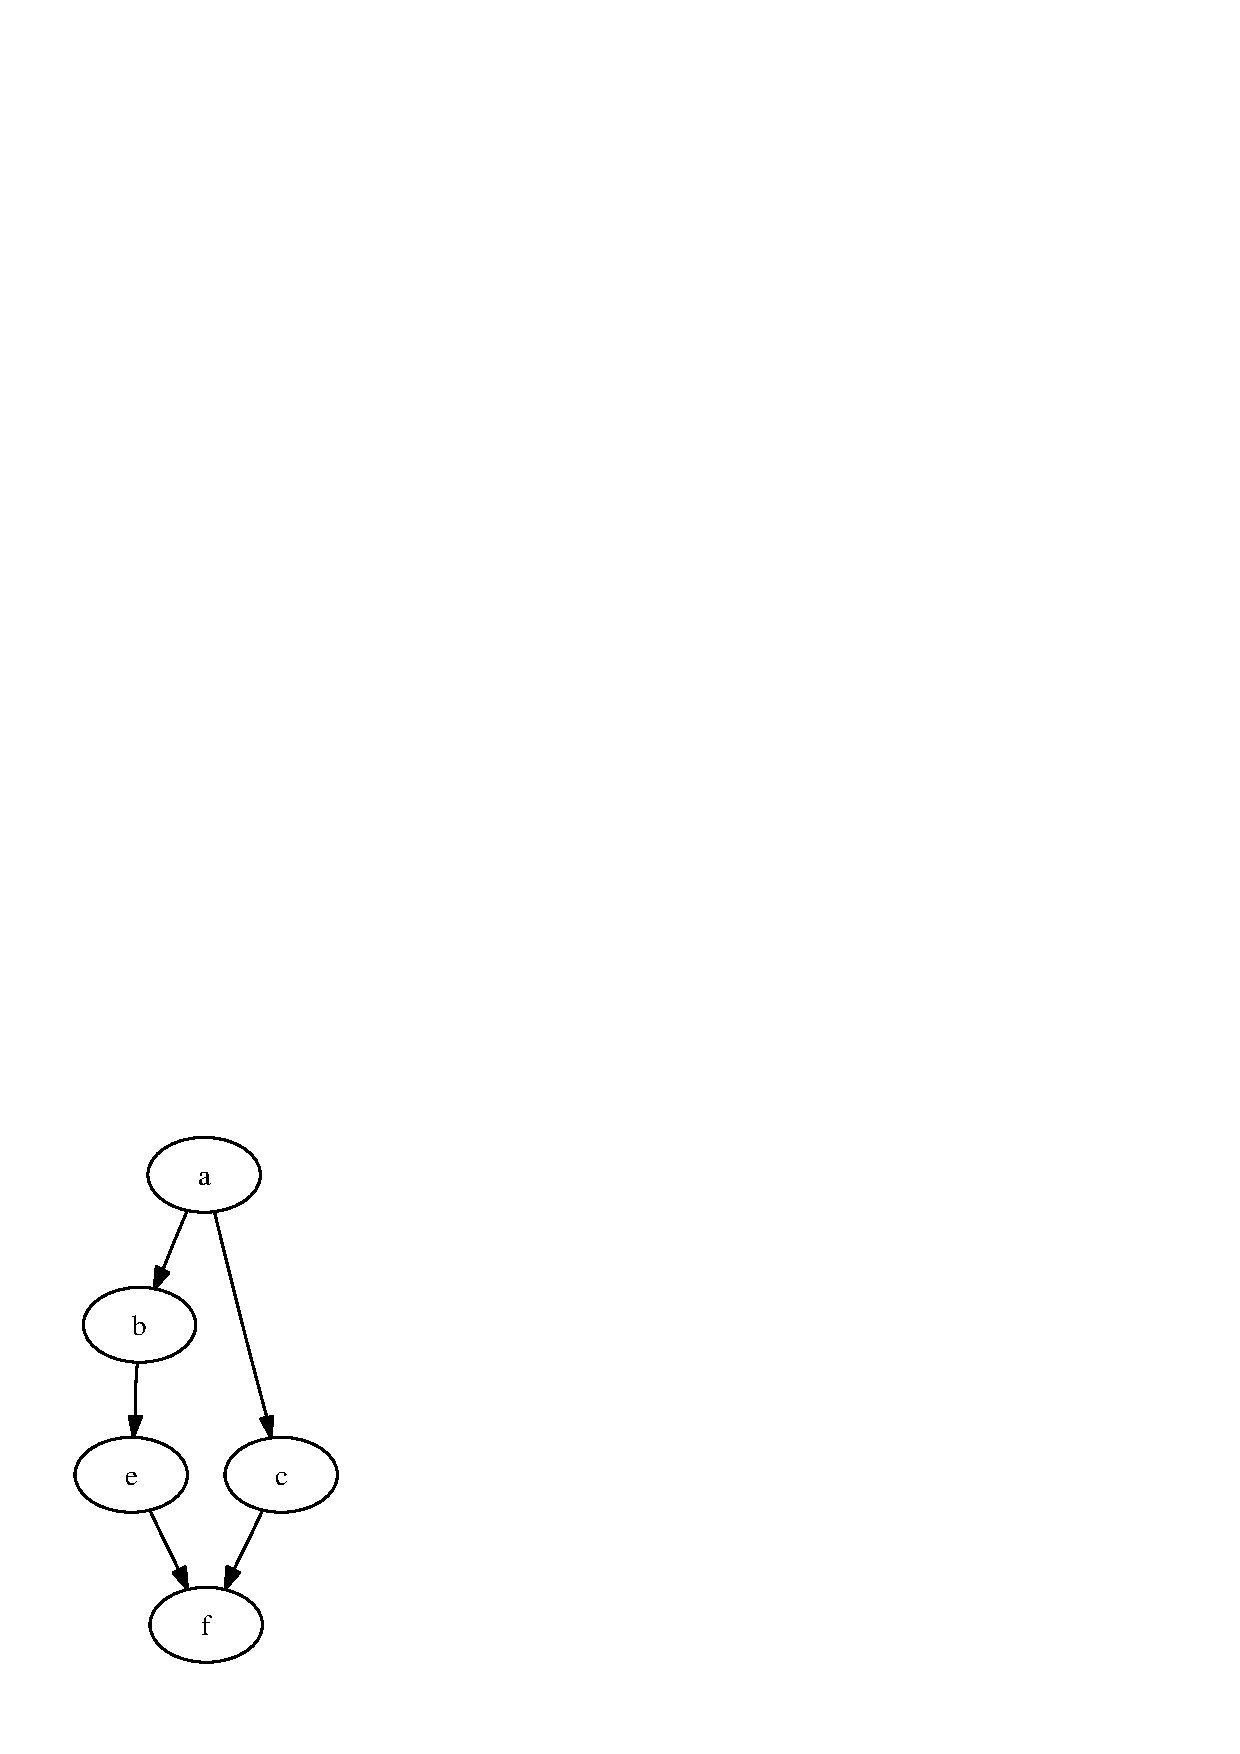
\epsfig{file=Figures/graph,scale=0.5}
  \caption{Ein einfacher Graph ohne Zykeln}
  \label{fig:graph}
\end{figure}

Wir wollen nun ein \textsl{Prolog}-Programm entwickeln, mit dem es m�glich ist, f�r zwei
vorgegebene Knoten $x$ und $y$ zu entscheiden, ob es einen Weg von $x$ nach $y$ gibt.
Au�erdem soll dieser Weg dann als Liste von Knoten berechnet werden.
Unser erster Ansatz besteht aus dem Programm, das in Abbildung \ref{fig:connect} gezeigt
ist.  Die Idee ist, dass der Aufruf \\[0.1cm]
\hspace*{1.3cm} \texttt{find\_path(\textsl{Start}, \textsl{Goal}, \textsl{Path})} \\[0.1cm]
einen Pfad \textsl{Path} berechnet, der von \textsl{Start} nach \textsl{Goal} f�hrt.  Wir diskutieren
die Implementierung.

\begin{figure}[!h]
  \centering
\begin{Verbatim}[ frame         = lines, 
                  framesep      = 0.3cm, 
                  labelposition = bottomline,
                  numbers       = left,
                  numbersep     = -0.2cm,
                  xleftmargin   = 0.8cm,
                  xrightmargin  = 0.8cm
                ]
    % find_path( +Point, +Point, -List(Point) ).
    find_path( X, X, [ X ] ).
    
    find_path( X, Z, [ X | Path ] ) :-
        edge( X, Y ),
        find_path( Y, Z, Path ).
\end{Verbatim}
\vspace*{-0.3cm}
  \caption{Berechnung von Pfaden in einem Graphen}
  \label{fig:connect}
\end{figure}

\begin{enumerate}
\item Die erste Klausel sagt aus, dass es trivialerweise einen Pfad von \texttt{X} nach
      \texttt{X} gibt.  Dieser Pfad enth�lt genau den Knoten \texttt{X}.
\item Die zweite Klausel sagt aus, dass es einen Weg von \texttt{X} nach \texttt{Z}
      gibt, wenn es zun�chst eine direkte Verbindung von \texttt{X} zu einem Knoten
      \texttt{Y} gibt und wenn es dann von diesem Knoten \texttt{Y} eine Verbindung
      zu dem Knoten \texttt{Z} gibt.  Wir erhalten den Pfad, der von \texttt{X} nach
      \texttt{Z} f�hrt, dadurch, dass wir vorne an den Pfad, der von \texttt{Y} nach \texttt{Z}
      f�hrt, den Knoten \texttt{X} anf�gen.
\end{enumerate}
Stellen wir an das \textsl{Prolog}-System die Anfrage \texttt{find\_path(a,f,P)}, so
erhalten wir die Antwort
\begin{Verbatim}[ frame         = lines, 
                  framesep      = 0.3cm, 
                  labelposition = bottomline,
                  numbers       = left,
                  numbersep     = -0.2cm,
                  xleftmargin   = 0.8cm,
                  xrightmargin  = 0.8cm
                ]
    ?- find_path(a,f,P).
 
    P = [a, b, e, f] ;   
    P = [a, c, f] ;
    No
\end{Verbatim}
Durch Backtracking werden also alle m�glichen Wege von \texttt{a} nach \texttt{b} gefunden.
Als n�chstes testen wir das Programm mit dem in Abbildung \ref{fig:graph2} gezeigten
Graphen.  Diesen Graphen stellen wir wie folgt in \textsl{Prolog} dar:
\begin{Verbatim}[ frame         = lines, 
                  framesep      = 0.3cm, 
                  labelposition = bottomline,
                  numbers       = left,
                  numbersep     = -0.2cm,
                  xleftmargin   = 0.8cm,
                  xrightmargin  = 0.8cm
                ]
    edge(a, b).
    edge(a, c).
    edge(b, e).
    edge(e, a).
    edge(e, f).
    edge(c, f).
\end{Verbatim}

\begin{figure}[!h]
  \centering
  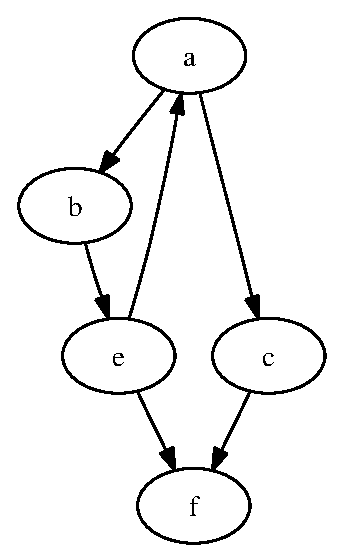
\epsfig{file=Figures/graph2,scale=0.5}
  \caption{Ein Graph mit einem Zykel}
  \label{fig:graph2}
\end{figure}

Jetzt erhalten wir auf die Anfrage \texttt{find\_path(a,f,P)} die Antwort
\begin{Verbatim}[ frame         = lines, 
                  framesep      = 0.3cm, 
                  labelposition = bottomline,
                  numbers       = left,
                  numbersep     = -0.2cm,
                  xleftmargin   = 0.8cm,
                  xrightmargin  = 0.8cm
                ]
    ?- find_path(a,f,P).
    ERROR: Out of local stack
\end{Verbatim}
Die Ursache ist schnell gefunden.
\begin{enumerate}
\item Wir starten mit der Anfrage \\[0.1cm]
      \hspace*{1.3cm} \texttt{find\_path(a,f,P)}.
\item Nach Unifikation mit der zweiten Klausel haben wir die Anfrage reduziert auf \\[0.1cm]
      \hspace*{1.3cm} 
      \texttt{edge( a, Y1 ), find\_path( Y1, f, P1 )}.
\item Nach Unifikation mit dem Fakt \texttt{edge(a,b)} haben wir die neue Anfrage \\[0.1cm]
      \hspace*{1.3cm} 
      \texttt{find\_path( b, f, P1 )}.
\item Nach Unifikation mit der zweiten Klausel haben wir die Anfrage reduziert auf \\[0.1cm]
      \hspace*{1.3cm} 
      \texttt{edge( b, Y2 ), find\_path( Y2, f, P2 )}.
\item Nach Unifikation mit dem Fakt \texttt{edge(b,e)} haben wir die neue Anfrage \\[0.1cm]
      \hspace*{1.3cm} 
      \texttt{find\_path( e, f, P2 )}.
\item Nach Unifikation mit der zweiten Klausel haben wir die Anfrage reduziert auf \\[0.1cm]
      \hspace*{1.3cm} 
      \texttt{edge( e, Y3 ), find\_path( Y3, f, P3 )}.
\item Nach Unifikation mit dem Fakt \texttt{edge(e,a)} haben wir die neue Anfrage \\[0.1cm]
      \hspace*{1.3cm} 
      \texttt{find\_path( a, f, P3 )}.
\end{enumerate}
Die Anfrage ``\texttt{find\_path(a, f, P3)}'' unterscheidet sich von der urspr�nglichen
Anfrage ``\texttt{find\_path(a,f,P)}'' nur durch den Namen der Variablen.  Wenn wir jetzt
weiterrechnen w�rden, w�rde sich die Rechnung nur wiederholen, ohne dass wir vorw�rts kommen.
Das Problem ist, das \textsl{Prolog} immer die erste
Klausel nimmt, die passt.  Wenn sp�ter die Reduktion der Anfrage scheitert, wird zwar nach
Backtracking die n�chste Klausel ausprobiert, aber wenn das Programm in eine
Endlos-Schleife l�uft, dann gibt es eben kein Backtracking, denn das Programm wei� ja
nicht, dass es in einer Endlos-Schleife ist.

Es ist leicht das Programm so umzuschreiben, dass keine Endlos-Schleife mehr
auftreten kann.  Die Idee ist, dass wir uns merken, welche Knoten wir bereits besucht
haben und diese nicht mehr ausw�hlen.  In diesem Sinne implementieren wir nun ein Pr�dikat \texttt{find\_path/4}.
Die Idee ist, dass der Aufruf \\[0.1cm]
\hspace*{1.3cm} \texttt{find\_path(\textsl{Start}, \textsl{Goal}, \textsl{Visited}, \textsl{Path})} \\[0.1cm]
einen Pfad berechnet, der von \textsl{Start} nach \textsl{Goal} f�hrt und der zus�tzlich
keine Knoten benutzt, die bereits in der Liste \textsl{Visited} aufgef�hrt sind.  Diese Liste
f�llen wir bei den rekursiven Aufrufen nach und nach mit den Knoten an, die wir bereits
besucht haben.  Mit Hilfe dieser Liste vermeiden wir es, einen Knoten zweimal zu besuchen.
Abbildung \ref{fig:connect2} zeigt die Implementierung.
\begin{figure}[!h]
  \centering
\begin{Verbatim}[ frame         = lines, 
                  framesep      = 0.3cm, 
                  labelposition = bottomline,
                  numbers       = left,
                  numbersep     = -0.2cm,
                  xleftmargin   = 0.8cm,
                  xrightmargin  = 0.8cm
                ]
    % find_path( +Point, +Point, +List(Point), -List(Point) )

    find_path( X, X, _Visited, [ X ] ).
    
    find_path( X, Z, Visited, [ X | Path ]) :-
        edge( X, Y ),
        \+ member( Y, Visited ),
        find_path( Y, Z, [ Y | Visited ], Path ).
    \end{Verbatim}
\vspace*{-0.3cm}
  \caption{Berechnung von Pfaden in zyklischen Graphen}
  \label{fig:connect2}
\end{figure}
\begin{enumerate}
\item In der ersten Klausel spielt das zus�tzliche Argument noch keine Rolle,
      denn wenn wir das Ziel erreicht haben, ist es uns egal, welche Knoten wir schon
      besucht haben.
\item In der zweiten Klausel �berpr�fen wir in Zeile 7, ob der Knoten \texttt{Y}
      in der Liste \textsl{Visited}, die die Knoten enth�lt, die bereits besucht wurden,
      auftritt.  Nur wenn dies nicht der Fall ist, versuchen wir rekursiv von \texttt{Y}
      einen Pfad nach \texttt{Z} zu finden.  Bei dem rekursiven Aufruf erweitern wir die Liste
      \texttt{Visited} um den Knoten \texttt{Y}, denn diesen Knoten wollen wir in Zukunft
      ebenfalls vermeiden.
\end{enumerate}
Mit dieser Implementierung ist es jetzt m�glich, auch in dem zweiten Graphen einen Weg von
\texttt{a} nach \texttt{f} zu finden, wir erhalten folgendes Ergebnis:
\pagebreak

\begin{Verbatim}[ frame         = lines, 
                  framesep      = 0.3cm, 
                  labelposition = bottomline,
                  numbers       = left,
                  numbersep     = -0.2cm,
                  xleftmargin   = 0.8cm,
                  xrightmargin  = 0.8cm
                ]
    ?- find_path(a,f,[a],P).
    P = [a, b, e, f] ;
    P = [a, c, f] ;    
    No
\end{Verbatim}


\subsection{Die Bekehrung der Ungl�ubigen}
Als spielerische Anwendung zeigen wir nun, wie sich mit Hilfe des oben definierten Pr�dikats 
\texttt{find\_path/4} ein theologisches Problem l�sen l�sst.
\vspace*{0.3cm}

\begin{minipage}[c]{14cm}
{\sl Drei Missionare und drei Ungl�ubige wollen zusammen einen Fluss 
�berqueren. Sie haben nur ein Boot, indem maximal zwei Passagiere fahren k�nnen.  
Sowohl die Ungl�ubigen als auch die Missionare k�nnen rudern.
Weder die Gl�ubigen, noch die Ungl�ubigen k�nnen �ber das Wasser laufen.
Die Ungl�ubigen sind hungrig, wenn die Missionare an einem der Ufer in der Unterzahl sind, 
haben sie ein Problem.  Die Aufgabe besteht darin, einen Fahrplan zu 
erstellen, so dass hinterher alle das andere  Ufer erreichen und die
Missionare zwischendurch kein Problem haben.}
\end{minipage}
\vspace*{0.4cm}

\noindent
Die Idee ist, das R�tsel, durch einen Graphen zu modellieren.  Die Knoten dieses 
Graphen sind dann die Situationen, die w�hrend des �bersetzens auftreten.  Wir
repr�sentieren diese Situationen durch Terme der Form \\[0.1cm]
\hspace*{1.3cm} $\texttt{side}(M,\;K,\;B)$.
\\[0.1cm]
Ein solcher Term repr�sentiert eine Situation, bei der auf der linken Seite des Ufers $M$ Missionare, $K$
Ungl�ubige und $B$ Boote sind.  Unsere Aufgabe besteht nun darin, das Pr�dikat
\texttt{edge/2} so zu implementieren, dass \\[0.1cm]
\hspace*{1.3cm} $\texttt{edge}(\;\texttt{side}(M_1,\;K_1,\;B_1),\;\texttt{side}(M_2,\;K_2,\;B_2)\;)$
\\[0.1cm]
genau dann wahr ist, wenn die Situation $\texttt{side}(M_1,\;K_1,\;B_1)$
durch eine Boots-�berfahrt in die Situation $\texttt{side}(M_2,\;K_2,\;B_2)$ �berf�hrt
werden kann und wenn zus�tzlich die Missionare in der neuen Situation kein Problem bekommen.
Abbildung \ref{fig:missionare.pl} auf Seite \pageref{fig:missionare.pl}
zeigt ein \textsl{Prolog}-Programm, was das R�tsel l�st.  Den von diesem Programm
berechneten Fahrplan finden Sie in Abbildung \ref{fig:missionare-solution} 
auf Seite \pageref{fig:missionare-solution}.
Wir diskutieren dieses Programm nun Zeile f�r Zeile.

\begin{figure}[!h]
  \centering
\begin{Verbatim}[ frame         = lines, 
                  framesep      = 0.3cm, 
                  labelposition = bottomline,
                  numbers       = left,
                  numbersep     = -0.2cm,
                  xleftmargin   = 0.8cm,
                  xrightmargin  = 0.8cm
                ]
    MMM   KKK   B      |~~~~~|                   
                       >  KK >
    MMM   K            |~~~~~|      B    KK      
                       <  K  <
    MMM   KK    B      |~~~~~|            K      
                       >  KK >
    MMM                |~~~~~|      B   KKK      
                       <  K  <
    MMM   K     B      |~~~~~|           KK      
                       > MM  >
    M     K            |~~~~~|      B    KK    MM
                       < M K <
    MM    KK    B      |~~~~~|            K     M
                       > MM  >
          KK           |~~~~~|      B     K   MMM
                       <  K  <
          KKK   B      |~~~~~|                MMM
                       >  KK >
          K            |~~~~~|      B    KK   MMM
                       <  K  <
          KK    B      |~~~~~|            K   MMM
                       >  KK >
                       |~~~~~|      B   KKK   MMM
\end{Verbatim}
\vspace*{-0.3cm}
  \caption{Fahrplan f�r Missionare und Ungl�ubige}
  \label{fig:missionare-solution}
\end{figure}      

\begin{figure}[!h]
  \centering
\begin{Verbatim}[ frame         = lines, 
                  framesep      = 0.3cm, 
                  labelposition = bottomline,
                  numbers       = left,
                  numbersep     = -0.2cm,
                  xleftmargin   = 0.8cm,
                  xrightmargin  = 0.8cm
                ]
    solve :-
        find_path( side(3,3,1), side(0,0,0), [ side(3,3,1) ], Path ),
        nl, write('L�sung:' ), nl, nl,
        print_path(Path).
    
    % edge( +Point, -Point ).    
    % This clause describes rowing from the left side to the right side.
    edge( side( M, K, 1 ), side( MN, KN, 0 ) ) :-
        between( 0, M, MB ),    % MB missionaries in the boat
        between( 0, K, KB ),    % KB infidels in the boat
        MB + KB >= 1,           % boat must not be empty
        MB + KB =< 2,           % no more than two passengers
        MN is M - MB,           % missionaries left on the left side
        KN is K - KB,           % infidels left on the left side
        \+ problem( MN, KN ).   % no problem must occur
    
    % This clause describes rowing from the right side to the left side.
    edge( side( M, K, 0 ), side( MN, KN, 1 ) ) :-
        otherSide( M, K, MR, KR ),
        edge( side( MR, KR, 1 ), side( MRN, KRN, 0 ) ),
        otherSide( MRN, KRN, MN, KN ).
    
    % otherSide( +Number, +Number, -Number, -Number ).
    otherSide( M, K, M_Other, K_Other ) :-
        M_Other is 3 - M,
        K_Other is 3 - K.
    
    % problem( +Number, +Number).
    problem(M, K) :- 
            problemSide(M, K).
    
    problem(M, K) :-
        otherSide( M, K, M_Other, K_Other ),
        problemSide(M_Other, K_Other).
        
    % problemSide( +Number, +Number).
    problemSide(Missionare, Kannibalen) :- 
            Missionare > 0, 
            Missionare < Kannibalen.
    
    % find_path( +Point, +Point, +List(Point), -List(Point) )
    find_path( X, X, _Visited, [ X ] ).
    
    find_path( X, Z, Visited, [ X | Path ]) :-
            edge( X, Y ),
            \+ member( Y, Visited ),
            find_path( Y, Z, [ Y | Visited ], Path ).
\end{Verbatim}
\vspace*{-0.3cm}
  \caption{Die Bekehrung der Ungl�ubigen}
  \label{fig:missionare.pl}
\end{figure}      

\begin{enumerate}
\item Wir beginnen mit dem  Hilfs-Pr�dikat \texttt{otherSide/4}, das in den
      Zeilen 24 -- 26 implementiert ist.  F�r eine vorgegebene Situation
      $\texttt{side}(M,K,B)$ berechnet der Aufruf \\[0.1cm]
      \hspace*{1.3cm} $\texttt{otherSide}(\; \texttt{side}(M, K, B),\; \textsl{OtherSide} \;)$
      \\[0.1cm] 
      einen Term, der die Situation am gegen�berliegenden Ufer beschreibt.
      Wenn an einen Ufer $M$ Missionare sind, so sind am anderen Ufer die restlichen
      Missionare und da es insgesamt $3$ Missionare gibt, sind das $3 - M$.
      Die Anzahl der Ungl�ubige am gegen�berliegenden Ufer wird analog berechnet. 
\item Das Pr�dikat \texttt{problem/2} in den Zeilen 29 -- 34 �berpr�ft, ob es bei einer vorgegeben
      Anzahl von Missionaren und Ungl�ubige zu einem Problem kommt.
      Da das Problem entweder am linken oder am rechten Ufer auftreten kann,
      besteht die Implementierung aus zwei Klauseln.  Die erste Klausel pr�ft,
      ob es auf der Seite, an der $M$ Missionare und $K$ Ungl�ubige sind, zum Problem
      kommt.  Die zweite Klausel �berpr�ft, ob es auf dem gegen�berliegenden
      Ufer zu einem Problem kommt.  Als Hilfs-Pr�dikat verwenden wir hier das Pr�dikat
      \texttt{problemSide/2}.  Dieses Pr�dikat ist in Zeile 37 implementiert
      und �berpr�ft die Situation an einer Seite:  Falls sich auf einer Seite $M$ Missionare
      und $K$ Ungl�ubige befinden, so gibt es dann ein Problem, wenn die Zahl $M$ von 0
      verschieden ist und wenn zus�tzlich $M < K$ ist.
\item Bei der Implementierung des Pr�dikats \texttt{edge/2} verwenden wir in den Zeilen 9
      und 10 das Pr�dikat \texttt{between/3}, das in dem \textsl{SWI-Prolog}-System 
      vordefiniert ist.  Beim Aufruf \\[0.1cm]
      \hspace*{1.3cm} $\texttt{between}(\textsl{Low}, \textsl{High}, N)$ \\[0.1cm]
      sind \textsl{Low} und \textsl{High} ganze Zahlen mit $\textsl{Low} \leq \textsl{High}$.
      Der Aufruf instantiert die Variable $N$ nacheinander mit den Zahlen \\[0.1cm]
      \hspace*{1.3cm} $\textsl{Low},\; \textsl{Low}+1,\; \textsl{Low}+2, \cdots, \;\textsl{High}$. \\[0.1cm]
      Beispielsweise gibt die Anfrage \\[0.1cm]
      \hspace*{1.3cm} \texttt{between(1,3,N), write(N), nl, fail.}  \\[0.1cm]
      nacheinander die Zahlen 1, 2 und 3 am Bildschirm aus.
    \item Die Implementierung des Pr�dikats \texttt{edge/2} besteht aus zwei Klauseln.  In
      der ersten Klausel betrachten wir den Fall, dass das Boot am linken Ufer ist.  In
      der Zeilen 9 generieren wir die Zahl der Missionare $\texttt{MB}$, die im Boot �bersetzen
      sollen.  Diese Zahl $\texttt{MB}$ ist durch $\texttt{M}$ beschr�nkt, denn es k�nnen nur die Missionare
      �bersetzen, die sich am linken Ufer befinden.  Daher benutzen wir das Pr�dikat
      \texttt{between/3} um eine Zahl zwischen 0 und $\texttt{M}$ zu erzeugen.  Analog generieren
      wir in Zeile 10 die Zahl $\texttt{KB}$ der Ungl�ubige, die im Boot �bersetzen.  In Zeile 11
      testen wir, dass es mindestens einen Passagier gibt, der mit dem Boot �bersetzt und
      in Zeile 12 testen wir, dass es h�chstens zwei Passagiere sind.  In Zeile 13 und 14
      berechnen wir die Zahl $\texttt{MN}$ der Missionare und die Zahl $\texttt{KN}$ der Ungl�ubige, die
      nach der �berfahrt auf dem linken Ufer verbleiben und testen dann in Zeile 15, dass es
      f�r diese Zahlen kein Problem gibt.
      
      Die zweite Klausel befasst sich mit dem Fall, dass das Boot am rechten Ufer liegt.
      Wir h�tten diese Klausel mit \textsl{Copy \& Paste} aus der vorhergehenden Klausel
      erzeugen k�nnen, aber es ist eleganter, diesen Fall auf den vorhergehenden Fall
      zur�ck zu f�hren.  Da da Boot nun auf der rechten Seite liegt, berechnen wir daher
      in Zeile 19 die Zahl $\texttt{MR}$ der Missionare auf der rechten Seite und die Zahl
      $\texttt{KR}$ der Ungl�ubige auf der rechten Seite.  Dann untersuchen wir die
      Situation $\mathtt{side}(\mathtt{MR}, \mathtt{KR}, 1)$, bei der $\texttt{MR}$
      Missionare und $\texttt{KR}$ Ungl�ubige am linken Ufer stehen.  Wenn diese so
      �bersetzen k�nnen, dass nachher $\texttt{MRN}$ Missionare und $\texttt{KRN}$
      Ungl�ubige am linken Ufer stehen, dann k�nnen wir in Zeile 21 berechnen, wieviele
      Missionare und Ungl�ubige sich dann am gegen�berliegenden Ufer befinden.
\item In den Zeilen 1 -- 4 definieren wir nun das Pr�dikat \texttt{solve/0}, dessen Aufruf
      das Problem l�st.  Dazu wird zun�chst das Pr�dikat \texttt{find\_path/4} 
      mit dem Start-Knoten \texttt{side(3,3,1)} und dem Ziel-Knoten \texttt{side(0,0,0)}
      aufgerufen.   Der berechnete Pfad wird dann ausgegeben mit dem Pr�dikat
      \texttt{print\_path/1},
      dessen Implementierung hier aus Platzgr�nden nicht angegeben wird.
\end{enumerate}


%%% Local Variables: 
%%% mode: latex
%%% TeX-master: "logik"
%%% End: 


\bibliographystyle{alpha}
\bibliography{/Users/stroetma/Kurse/cs}

\end{document}



%%% Local Variables: 
%%% mode: latex
%%% TeX-master: "logic"
%%% End: 
